\section{Lí thuyết cấu trúc của chất}
\loai{Loại 1: Chuyển động Brown}
\begin{ex}%chuan
	Thí nghiệm của Brown quan sát
	\choice
	{hạt phấn hoa bằng kính hiển vi}
	{\True chuyển động của hạt phấn hoa trong nước bằng kính hiển vi}
	{cánh hoa trong nước bằng kính hiển vi}
	{chuyển động của cánh hoa}
	\loigiai{
		\begin{itemize}
			\item Thí nghiệm của Brown quan sát chuyển động của các hạt phấn hoa trong nước, thấy các hạt phấn chuyển động hỗn độn, không ngừng
		\end{itemize}
	}
	\haidong{3}
\end{ex}






\loai{Loại 2: Cấu tạo chất}
\begin{ex}%chuan
	Phát biểu nào sau đây là \textbf{sai} khi nói về cấu tạo chất?	
	\choice
	{Các phân tử luôn luôn chuyển động không ngừng}
	{Các phân tử chuyển động càng nhanh thì nhiệt độ của vật càng cao}
	{\True Các phân tử luôn luôn đứng yên và chỉ chuyển động khi nhiệt độ của vật cao}
	{Các chất được cấu tạo từ các hạt riêng biệt gọi là phân tử}
	\loigiai{
		\begin{itemize}
			\item Các phân tử chuyển động không ngừng.
			Chuyển động của các phân tử được gọi là chuyển động nhiệt.
		\end{itemize}
	}
	\haidong{2}\end{ex}




\loai{Loại 3: Mô hình động học phân tử}


\begin{ex}%chuan
	Phát biểu nào sau đây \textbf{không} đúng với mô hình động học phân tử?
	
	\choice
	{Các chất được cấu tạo từ các hạt riêng biệt là phân tử}
	{Các phân tử chuyển động không ngừng}
	{\True Tốc độ chuyển động của các phân tử cấu tạo nên vật càng lớn thì thể tích của vật càng lớn}
	{Giữa các phân tử có lực tương tác gọi là lực liên kết phân tử}
	\loigiai{
		\begin{itemize}
			\item Các phân tử chuyển động càng nhanh thì nhiệt độ của vật do chúng tạo nên càng cao
		\end{itemize}
		
	}
	\haidong{2}\end{ex}





\begin{ex}%chuan \nguon{4}
	Phát biểu nào sau đây là đúng khi nói về mô hình động học phân tử?
	\choice
	{Các phân tử cấu tạo nên các chất luôn đứng yên tại một vị trí cố định}
	{\True Các phân tử cấu tạo nên các chất luôn chuyển động không ngừng}
	{Các phân tử cấu tạo nên các chất có thể chuyển động hoặc đứng yên tùy vào đó là chất rắn, chất lỏng hay chất khí}
	{Các phân tử cấu tạo nên chất lỏng và chất khí thì chuyển động, các hạt cấu tạo nên chất rắn thì đứng yên}
	\loigiai{
		\begin{itemize}
			\item Theo mô hình động học phân tử, các phân tử cấu tạo nên các chất luôn chuyển động không ngừng.
			\item Chuyển động của các phân tử xảy ra ngay cả trong trạng thái rắn, lỏng và khí, mặc dù theo những cách khác nhau.
		\end{itemize}
	}
\end{ex}



\begin{ex}%chuan \nguon{4}
	Mô hình động học phân tử được xây dựng dựa trên quan điểm nào về cấu tạo chất?
	\choice
	{Dựa trên quan điểm chất có cấu tạo liên tục}
	{\True Dựa trên quan điểm chất có cấu tạo gián đoạn}
	{Dựa trên cả hai quan điểm là chất có cấu tạo liên tục và gián đoạn}
	{Dựa trên quan điểm về sự bền vững của các phân tử}
	\loigiai{
		\begin{itemize}
			\item Mô hình động học phân tử được xây dựng dựa trên quan điểm chất có cấu tạo gián đoạn.
			\item Theo quan điểm này, chất được cấu tạo từ các phân tử rời rạc, không liên tục và luôn chuyển động.
		\end{itemize}
	}
\end{ex}



\begin{ex}%chuan \nguon{1}
	Phát biểu nào sau đây \textbf{không} đúng?
	\choice
	{Các chất được cấu tạo từ các hạt gọi là phân tử}
	{Lực tương tác giữa các phân tử ở thể rắn lớn hơn lực tương tác giữa các phân tử ở thể lỏng và thể khí}
	{Các phân tử chất lỏng dao động xung quanh các vị trí cân bằng không cố định}
	{\True Các phân tử đứng sát nhau và giữa chúng không có khoảng cách}
	\loigiai{
		\begin{itemize}
			\item Phát biểu "Các phân tử đứng sát nhau và giữa chúng không có khoảng cách" là không đúng. Trong thực tế, ngay cả khi các phân tử ở gần nhau nhất, giữa chúng vẫn tồn tại khoảng cách nhất định do sự tồn tại của các lực tương tác và các quy luật cơ học lượng tử. 
			\item Những phát biểu còn lại đều đúng:
			\begin{itemize}
				\item "Các chất được cấu tạo từ các hạt gọi là phân tử" là đúng vì theo mô hình cấu tạo của vật chất, tất cả các chất đều được cấu thành từ các phân tử.
				\item "Lực tương tác giữa các phân tử ở thể rắn lớn hơn lực tương tác giữa các phân tử ở thể lỏng và thể khí" là đúng vì ở thể rắn, các phân tử sắp xếp gần nhau và có lực hút lớn, tạo thành cấu trúc cố định, trong khi ở thể lỏng và thể khí, các lực tương tác yếu hơn.
				\item "Các phân tử chất lỏng dao động xung quanh các vị trí cân bằng không cố định" cũng là đúng vì trong chất lỏng, các phân tử có vị trí cân bằng thay đổi liên tục do chúng có thể trượt qua nhau nhưng không tách rời hoàn toàn.
			\end{itemize}
		\end{itemize}
	}
\end{ex}









\loai{Loại 4: Lực tương tác phân tử}


\begin{ex}%chuan
	Lực liên kết giữa các phân tử	
	\choice
	{là lực hút}
	{là lực đẩy}
	{tuỳ thuộc vào thể của nó, ở thể rắn là lực hút còn ở thể khí là lực đẩy}
	{\True gồm cả lực hút và lực đẩy}
	\loigiai{
		\begin{itemize}
			\item Giữa các phân tử có lực hút và lực đẩy, gọi chung là lực liên kết phân tử.
		\end{itemize}
	}
	\haidong{2}\end{ex}



\begin{ex}%chuan%[1P5B1-1][Loai1]
	Phát biểu nào sau đây nói về lực tương tác phân tử là \textbf{không} đúng?
	\choice
	{Lực tương tác phân tử đáng kể khi các phân tử ở rất gần nhau}
	{Lực hút phân tử có thể lớn hơn lực đẩy phân tử}
	{\True Lực hút phân tử không thể lớn hơn lực đẩy phân tử}
	{Lực hút phân tử có thể bằng lực đẩy phân tử}
	\loigiai{
		\begin{itemize}
			\item Giữa các phân tử luôn có cả lực hút và lực đẩy. Lực hút và sẽ lớn hơn hay nhỏ hơn lực đẩy tùy vào khoảng cách giữa các phân tử.
	\end{itemize}} 
	%<MyLT3>
	\haidong{2}\end{ex}


\loai{Loại 5. Chuyển động nhiệt của phân tử}

\begin{ex}%chuan
	Phát biểu nào sau đây nói về chuyển động của phân tử là \textbf{không} đúng?
	\choice
	{\True Chuyển động của phân tử hoàn toàn là do lực tương tác phân tử gây ra}
	{Các phân tử chuyển động không ngừng}
	{Các phân tử chuyển động càng nhanh thì nhiệt độ của vật càng cao}
	{Các phân tử khí chuyển hỗn loạn không ngừng về mọi hướng}
	\loigiai{
		\begin{itemize}
			\item Giữa các phân tử có lực hút và lực đẩy, gọi chung là lực liên kết phân tử.
			\item Lực tương tác phân tử có thể gây thay đổi chuyển động chứ không gây ra chuyển động.
		\end{itemize}
	}
	\haidong{2}
\end{ex}







\begin{ex}%chuan \nguon{1}
	Phát biểu nào sau đây là đúng?
	\choice
	{Ở cùng nhiệt độ, các phân tử của các chất khác nhau sẽ có vận tốc chuyển động giống nhau}
	{Các nguyên tử, phân tử cấu tạo nên vật không chuyển động}
	{\True Nhiệt độ càng cao thì các nguyên tử, phân tử chuyển động càng nhanh}
	{Các vật được cấu tạo liền một khối}
	\loigiai{
		\begin{itemize}
			\item Phát biểu đúng là "Nhiệt độ càng cao thì các nguyên tử, phân tử chuyển động càng nhanh". Điều này dựa trên nguyên lý cơ bản của thuyết động học phân tử, theo đó khi nhiệt độ tăng, các phân tử sẽ chuyển động nhanh hơn.		
			\item Phát biểu “Ở cùng nhiệt độ, các phân tử của các chất khác nhau sẽ có vận tốc chuyển động giống nhau” không hoàn toàn chính xác, vì vận tốc trung bình của phân tử phụ thuộc chủ yếu vào khối lượng phân tử và nhiệt độ, không chỉ riêng nhiệt độ.		
			\item Phát biểu “Các nguyên tử, phân tử cấu tạo nên vật không chuyển động” là sai, vì trong thực tế, các nguyên tử và phân tử luôn có chuyển động nhiệt.		
			\item Phát biểu “Các vật được cấu tạo liền một khối” cũng là không đúng, vì các vật thực tế được tạo thành từ các nguyên tử và phân tử riêng biệt.
			\item Do đó, đáp án chính xác là “Nhiệt độ càng cao thì các nguyên tử, phân tử chuyển động càng nhanh”.
		\end{itemize}
	}
\end{ex}
\loai{Loại 6: Xác định các thể}




\begin{ex}%chuan
	Các chất có thể tồn tại ở những thể cơ bản nào?
	\choice
	{Thể rắn}
	{Thể lỏng}
	{Thể khí}
	{\True Thể rắn, thể lỏng, thể khí}
	\loigiai{
		\begin{itemize}
			\item Ba thể cơ bản của các chất: Thể rắn, thể lỏng, thể khí
		\end{itemize}
	}
	\haidong{3}\end{ex}

\begin{ex}%chuan
	Chất nào sau đây có thể tồn tại ở cả ba thể rắn, lỏng, khí ở điều kiện tự nhiên trên Trái Đất?
	
	\choice
	{\True Nước}
	{Oxygen}
	{Nitrogen}
	{Carbon dioxide}
	\loigiai{
		
		\begin{itemize}
			\item Nước có thể tồn tại ở thể rắn (nước đá, băng, tuyết), thể lỏng (nước lỏng), thể khí (hơi nước).
		\end{itemize}
		
	}
	\haidong{2}\end{ex}



\begin{ex}%chuan
	Chất nào sau đây ở thể khí khi ở điều kiện thường?
	
	\choice
	{Muối ăn}
	{Đường}
	{Giấm}
	{\True Carbon dioxide}
	\loigiai{
		
		\begin{itemize}
			\item 	Carbon dioxide là chất khí ở điều kiện thường.
		\end{itemize}
		
	}
	\haidong{2}\end{ex}








\loai{Loại 7: Cấu trúc chất rắn}

%


\begin{ex}%chuan
	Vật rắn có hình dạng xác định vì phân tử cấu tạo nên vật rắn
	\choice
	{không chuyển động}
	{đứng sát nhau}
	{chuyển động với vận tốc nhỏ không đáng kể}
	{\True chuyển động quanh một vị trí cân bằng xác định}
	\loigiai{
		\begin{itemize}
			\item Các phân tử chất rắn được giữ ở các vị trí cân bằng và mỗi phân tử chỉ có thể dao động xung quanh vị trí cân bằng xác định này nên các chất ở thể rắn có thể tích và hình dạng xác định.
		\end{itemize}
	}
	\haidong{2}\end{ex}

\begin{ex}%chuan
	Tại sao người ta \textbf{không} nén chất rắn lại để tiết kiệm diện tích?
	\choice
	{\True Do chất rắn liên kết chặt chẽ với nhau nên rất khó nén}
	{Do chất rắn liên kết không chặt chẽ với nhau nên khó nén}
	{Do các hạt của chất rắn chuyển động tự do}
	{Do người ta không muốn nén chất rắn}
	\loigiai{
		\begin{itemize}
			\item Trong chất rắn, các phân tử ở rất gần nhau nên lực tương tác giữa các phân tử chất rắn chặt chẽ, do đó nó có thể tích xác định và không thể nén được.
		\end{itemize}
	}
	\haidong{2}\end{ex}

\begin{ex}%chuan
	Những đặc điểm nào sau đây là của chất rắn?
	\choice
	{Có khối lượng và hình dạng xác định, không có thể tích xác định}
	{Có khối lượng xác định, hình dạng và thể tích không xác định}
	{\True Có khối lượng, hình dạng và thể tích xác định}
	{Có khối lượng và thể tích xác định, hình dạng không xác định}
	\loigiai{
		\begin{itemize}
			\item Các phân tử chất rắn được giữ ở các vị trí cân bằng và mỗi phân tử chỉ có thể dao động xung quanh vị trí cân bằng xác định này nên các chất ở thể rắn có thể tích và hình dạng xác định.
		\end{itemize}
	}
	\haidong{2}\end{ex}



\begin{ex}%chuan
	Các nguyên tử trong một miếng sắt có tính chất nào sau đây?
	\choice
	{Khi nhiệt độ tăng thì nở ra}
	{Khi nhiệt độ giảm thì co lại}
	{\True Khoảng cách rất gần nhau}
	{Khoảng cách rất xa nhau}
	\loigiai{
		\begin{itemize}
			\item Các nguyên tử trong kim loại nói riêng và chất rắn nói chung thường đứng rất gần nhau.
		\end{itemize}		
	}
	\haidong{2}\end{ex}

\loai{Loại 8: Chất rắn kết tinh}


\begin{ex}%chuan
	Trong các chất sau, chất nào \textbf{không} phải là chất rắn kết tinh?
	\choice
	{Muối ăn}
	{\True Thuỷ tinh}
	{Kim cương}
	{Thạch anh}
	\loigiai{
		\begin{itemize}
			\item Thủy tinh không có cấu trúc tinh thể, là chất rắn vô định hình
		\end{itemize}
	}
	\haidong{2}\end{ex}









\begin{ex}%chuan \nguon{1}
	Trong tinh thể, các hạt (nguyên tử, phân tử, ion)
	\choice
	{\True dao động nhiệt xung quanh vị trí cân bằng}
	{đứng yên tại những vị trí xác định}
	{chuyển động hỗn độn không ngừng}
	{chuyển động trên quỹ đạo tròn xung quanh một vị trí xác định}
	\loigiai{
		\begin{itemize}
			\item Trong tinh thể, các nguyên tử, phân tử, hoặc ion không đứng yên mà dao động xung quanh các vị trí cân bằng của chúng. 
			\item Vị trí cân bằng này là các vị trí cấu trúc xác định mà các hạt chiếm giữ. Khi nhiệt độ tăng, dao động nhiệt của các hạt tăng lên, nhưng chúng vẫn dao động xung quanh vị trí cân bằng cố định. 
			\item Đây là lý do vì sao tinh thể có hình dạng và cấu trúc ổn định ở điều kiện bình thường.
		\end{itemize}
	}
\end{ex}





\begin{ex}%chuan \nguon{4}
	Khi chất rắn kết tinh được nung nóng. Phát biểu nào sau đây là đúng?
	\choice
	{các phân tử vẫn dao động với biên độ không đổi, khoảng cách trung bình giữa các phân tử không đổi}
	{\True các phân tử dao động với biên độ tăng lên, khoảng cách trung bình giữa các phân tử tăng lên}
	{các phân tử dao động với biên độ không đổi, khoảng cách trung bình giữa các phân tử tăng lên}
	{các phân tử dao động với biên độ tăng lên, khoảng cách trung bình giữa các phân tử không đổi}
	\loigiai{
		Khi nung nóng, các phân tử trong chất rắn dao động mạnh hơn (biên độ tăng), làm cho khoảng cách giữa các phân tử cũng tăng lên.
	}
\end{ex}


\loai{Loại 9: Chất rắn vô định hình}


\begin{ex}%chuan
	Chất rắn nào sau đây thuộc dạng chất rắn vô định hình?
	\choice
	{Muối ăn}
	{Kim loại}
	{Thạch anh}
	{\True Nhựa đường}
	\loigiai{
		\begin{itemize}
			\item Chất rắn vô định hình: Không có cấu trúc tinh thể.
			\item Thuỷ tinh, nhựa đường, cao su,... là những chất rắn vô định hình.
		\end{itemize}
	}
	\haidong{3}\end{ex}

\begin{ex}%chuan
	Chất rắn nào dưới đây thuộc loại chất rắn vô định hình?
	\choice
	{Ống nano carbon}
	{\True Socola}
	{Nhôm}
	{Kim cương}
	\loigiai{
		\begin{itemize}
			\item Chất rắn vô định hình: Không có cấu trúc tinh thể.
			Socola là chất rắn vô định hình
		\end{itemize}	
	}
	\haidong{3}\end{ex}


\loai{Loại 10: Chất rắn kết tinh – Chất rắn vô định hình}









\begin{ex}%chuan \nguon{1}
	Vật nào sau đây \textbf{không} có cấu trúc tinh thể?
	\choice
	{Hạt muối}
	{Viên kim cương}
	{Miếng thạch anh}
	{\True Chiếc cốc làm bằng thủy tinh}
	\loigiai{
		\begin{itemize}
			\item Trong số các vật được liệt kê, chiếc cốc làm bằng thủy tinh không có cấu trúc tinh thể. 
			\item Thủy tinh là một chất rắn vô định hình, nghĩa là các nguyên tử trong thủy tinh không sắp xếp theo một trật tự tuần hoàn và đều đặn như trong cấu trúc tinh thể. 
			\item Ngược lại, hạt muối, viên kim cương và miếng thạch anh đều có cấu trúc tinh thể, trong đó các nguyên tử hoặc ion được sắp xếp theo một mạng lưới đều đặn và lặp đi lặp lại.\end{itemize}
	}
\end{ex}




\loai{Loại 11: Cấu trúc chất lỏng}




\begin{ex}%chuan
	Đặc điểm nào sau đây là đặc điểm của chất lỏng?
	\choice
	{Có hình dạng của phần bình chứa nó, có thể rót được và chảy tràn trên bề mặt, dễ nén}
	{\True Có hình dạng của phần bình chứa nó, có thể rót được và chảy tràn trên bề mặt, rất khó nén}
	{Có hình dạng cố định, có thể rót được và chảy tràn trên bề mặt, rất khó nén}
	{Có hình dạng của phần bình chứa nó, dễ dàng lan tỏa trong không gian, dễ nén}
	\loigiai{
		\begin{itemize}
			\item Do lực liên kết giữa các phân tử yếu hơn trong chất rắn nên các chất ở thể lỏng có thể tích xác định nhưng không có hình dạng riêng mà có hình dạng của phần bình chứa nó.
		\end{itemize}
	}
	\haidong{2}\end{ex}

\begin{ex}%chuan
	Chất lỏng có thể tích xác định, nhưng hình dạng không xác định là do trong chất lỏng có những đặc điểm nào sau đây?
	\choice
	{Lực liên kết giữa các phân tử chất lỏng là rất lớn, các phân tử chỉ dao động không ngừng quanh một vị trí xác định}
	{Lực liên kết giữa các phân tử chất lỏng là rất yếu, các phân tử dao động tự do về mọi phía}
	{\True Lực liên kết giữa các phân tử trong chất lỏng yếu hơn so với chất rắn, các phân tử khi dao động còn có thể trượt lên nhau}
	{Lực liên kết giữa các phân tử chất lỏng là rất yếu, các phân tử dao động xung quanh một vị trí xác định}
	\loigiai{
		\begin{itemize}
			\item Lực liên kết giữa các phân tử yếu hơn trong chất rắn nên các chất ở thể lỏng có thể tích xác định nhưng không có hình dạng riêng mà có hình dạng
			của phần bình chứa nó
		\end{itemize}
	}
	\haidong{1}\end{ex}





\begin{ex}%chuan \nguon{4}
	Lực tương tác giữa các phân tử trong chất lỏng
	\choice
	{rất lớn và giữ cho các phân tử chất lỏng dao động tại vị trí cân bằng xác định}
	{rất yếu nên chất lỏng không có thể tích xác định}
	{\True vẫn đủ để giữ các phân tử không chuyển động phân tán ra xa nhau}
	{rất yếu nên chất lỏng rất dễ bị nén}\loigiai{
		Lực tương tác giữa các phân tử trong chất lỏng không mạnh như trong chất rắn nhưng đủ lớn để giữ cho các phân tử không chuyển động phân tán và giữ cho chất lỏng có thể tích xác định.
	}
\end{ex}

\begin{ex}%chuan \nguon{4}
	Chất lỏng có thể tích xác định vì
	\choice
	{các phân tử cấu tạo nên chất lỏng có thể chuyển động hỗn độn, tự do}
	{lực liên kết giữa các phân tử trong chất lỏng là rất yếu}
	{\True lực tương tác giữa các phân tử vẫn đủ để giữ các phân tử không chuyển động phân tán ra xa nhau}
	{vị trí cân bằng của các phân tử có thể chuyển động từ nơi này đến nơi khác}\loigiai{
		Lực tương tác giữa các phân tử trong chất lỏng đủ mạnh để giữ chúng lại gần nhau, tạo ra thể tích xác định cho chất lỏng mặc dù hình dạng của nó có thể thay đổi.
	}
\end{ex}

\begin{ex}%chuan \nguon{4}
	Chuyển động nào sau đây là chuyển động của riêng các phân tử ở thể lỏng?
	\choice
	{Chuyển động hỗn loạn không ngừng}
	{Dao động xung quanh các vị trí cân bằng cố định}
	{Chuyển động hoàn toàn tự do}
	{\True Dao động xung quanh các vị trí cân bằng không cố định}\loigiai{
		Các phân tử trong chất lỏng dao động quanh các vị trí cân bằng không cố định, cho phép chúng di chuyển linh hoạt và dễ dàng thay đổi vị trí.
	}
\end{ex}



\loai{Loại 12: Cấu trúc chất khí}




\begin{ex}%chuan%[1P5Y1-1][Loai2]
	Tính chất nào sau đây \textbf{không} phải là của phân tử vật chất ở thể khí?
	\choice
	{Chuyển động hỗn loạn}
	{Chuyển động không ngừng}
	{Chuyển động tự do về mọi phía}
	{\True Chuyển động hỗn loạn xung quanh các vị trí cân bằng cố định}
	\loigiai{
		\begin{itemize}
			\item Ở trạng thái khí, các phân tử chuyển động hỗn loạn và không có vị trí cân bằng.
		\end{itemize}
	} 
	%<MyLT3>
	\haidong{2}\end{ex}



\begin{ex}%chuan%[1P5Y1-1][Loai3]
	Phát biểu nào sau đây là đúng về chất khí?
	\choice
	{\True Chất khí không có hình dạng và thể tích riêng}
	{Chất khí luôn chiếm một phần thể tích của bình chứa}
	{Rất khó để nén được chất khí}
	{Chất khí có thể tích xác định}
	\loigiai{
		\begin{itemize}
			\item Do lực tương tác giữa các phân tử chất khí quá yếu nên chất khí không có hình dạng và thể tích riêng.
		\end{itemize}
	} 
	%<MyLT2>
	\haidong{3}\end{ex}




\begin{ex}%chuan
Các phân tử khí chuyển động hỗn loạn không ngừng vì
\choice
{phân tử khí không có khối lượng}
{khoảng cách giữa các phân tử khí quá gần nhau}
{\True lực tương tác giữa các phân tử quá nhỏ}
{các phân tử khí luôn đẩy nhau}
\loigiai{
	\begin{itemize}
		\item Khoảng cách giữa các phân tử rất lớn so với kích
		thước của chúng. Lực tương tác giữa các phân tử hầu như không đáng
		kể (trừ khi va chạm nhau) nên chúng chuyển động hỗn loạn không ngừng về mọi phía
	\end{itemize}
}
\haidong{2}\end{ex}

\begin{ex}%chuan
Tính chất nào sau đây \textbf{không} phải là tính chất của chất ở thể khí?

\choice
{\True Có hình dạng và thể tích riêng}
{Các phân tử chuyển động hoàn toàn hỗn độn}
{Có thể nén được dễ dàng}
{Có lực tương tác phân tử nhỏ hơn lực tương tác phân tử ở thể rắn và thể lỏng}
\loigiai{
	\begin{itemize}
		\item Các chất ở thể khí không có thể tích và hình dạng riêng mà có thể tích và hình dạng của bình chứa.
	\end{itemize}
}
\haidong{3}\end{ex}

\begin{ex}%chuan
Chất khí \textbf{không} có hình dạng và thể tích riêng là vì

\choice
{khoảng cách giữa các phân tử rất gần, lực tương tác giữa các phân tử chất khí rất mạnh}
{khoảng cách giữa các phân tử rất gần, lực tương tác giữa các phân tử chất khí rất yếu}
{khoảng cách giữa các phân tử rất xa, lực tương tác giữa các phân tử chất khí rất mạnh}
{\True khoảng cách giữa các phân tử rất xa, lực tương tác giữa các phân tử chất khí rất yếu}
\loigiai{
	\begin{itemize}
		\item  Khoảng cách giữa các phân tử rất lớn so với kích
		thước của chúng nên lực tương tác giữa các phân tử hầu như không đáng
		kể (trừ khi va chạm nhau) dẫn tới hệ quả trên.
	\end{itemize}
}
\haidong{4}\end{ex}





\begin{ex}%chuan \nguon{3}
Một bình nước hoa được mở nắp ở cuối lớp học nhưng ở mọi vị trí của lớp hầu như bạn nào cũng ngửi thấy được. Điều này thể hiện tính chất nào của thể khí?
\choice
{Dễ dàng nén được}
{Không có hình dạng xác định}
{\True Có thể lan toả trong không gian theo mọi hướng}
{Không chảy được}
\loigiai{
	Tính chất "Có thể lan toả trong không gian theo mọi hướng" của chất khí giải thích vì sao mọi người trong lớp đều ngửi thấy được mùi nước hoa khi bình nước hoa được mở nắp. Điều này là do các phân tử khí của nước hoa phân tán và di chuyển khắp phòng.
}
\end{ex}


\begin{ex}%chuan \nguon{4}
Phát biểu nào sau đây về các phân tử của chất khí là đúng?
\choice
{Các phân tử chất khí liên kết chặt chẽ với nhau}
{Các phân tử chất khí dao động quanh vị trí cân bằng cố định}
{\True Các phân tử chất khí chuyển động hỗn loạn, không ngừng về mọi phía}
{Các phân tử chất khí được sắp xếp rất gần nhau}
\loigiai{
	
	Các phân tử chất khí luôn chuyển động hỗn loạn và không ngừng về mọi phía, điều này làm cho chất khí có thể lan tỏa đều trong không gian chứa nó.
}
\end{ex}

\begin{ex}%chuan \nguon{4}
Tính chất nào sau đây \textbf{không} phải là của phân tử của các chất ở thể khí?
\choice
{Các phân tử liên kết với nhau rất yếu}
{Khoảng cách trung bình của các phân tử xa nhau}
{Chuyển động hỗn loạn và không ngừng}
{\True Chuyển động hỗn loạn xung quanh các vị trí cân bằng cố định}
\loigiai{
	
	Các phân tử khí không dao động xung quanh các vị trí cân bằng cố định. Thay vào đó, chúng chuyển động hỗn loạn và không ngừng trong không gian.
}
\end{ex}

\begin{ex}%chuan \nguon{4}
Chất khí \textbf{không} có thể tích riêng là vì
\choice
{các phân tử chất khí dao động quanh các vị trí cân bằng có thể di chuyển được}
{\True các phân tử chất khí chuyển động hỗn loạn về mọi phía}
{lực đẩy giữa các phân tử chất khí rất mạnh}
{khoảng cách giữa các phân tử chất khí rất nhỏ so với kích thước của chúng}
\loigiai{
	
	Các phân tử chất khí chuyển động hỗn loạn theo mọi hướng, khiến cho chất khí không có thể tích cố định hay hình dạng cố định.
}
\end{ex}


\loai{Loại 13: Tổng hợp các thể vật chất đơn giản}
\begin{ex}%chuan%[1P5B1-1][Loai2]
Phát biểu nào sau đây là \textbf{sai}?
\choice
{Các chất được cấu tạo một cách gián đoạn}
{Lực tương tác giữa các phân tử ở thể rắn lớn hơn lực tương tác giữa các phân tử ở thể lỏng và thể khí}
{\True Các phân tử chất rắn dao động quanh vị trí cân bằng không cố định}
{Giữa các phân tử đồng thời có cả lực hút và lực đẩy}
\loigiai{
	\begin{itemize}
		\item Ở trạng thái rắn, các nguyên tử, phân tử dao động quanh các vị trí cân bằng cố định.
	\end{itemize}
} %<MyLT1>
\haidong{2}\end{ex}




\begin{ex}%chuan \nguon{1}
Ở nhiệt độ phòng, chất nào ở thể lỏng?
\choice
{Chì}
{Kẽm}
{\True Thủy ngân}
{Thiếc}
\loigiai{
	\begin{itemize}
		\item Chất ở thể lỏng ở nhiệt độ phòng là: \emph{Thủy ngân}.
		
		\item Giải thích chi tiết:
		\begin{itemize}
			\item \textbf{Chì}: Ở nhiệt độ phòng, chì là chất rắn.
			\item \textbf{Kẽm}: Ở nhiệt độ phòng, kẽm là chất rắn.
			\item \textbf{Thủy ngân}: Đúng. Thủy ngân là một chất đặc biệt, ở thể lỏng tại nhiệt độ phòng (khoảng 25°C).
			\item \textbf{Thiếc}: Ở nhiệt độ phòng, thiếc là chất rắn.
	\end{itemize}\end{itemize}
}
\end{ex}




\loai{Loại 14: So sánh đặc điểm của các chất}
%\begin{ex}%chuan%[1P5Y1-1][Loai2]
%	Trong các tính chất sau, tính chất nào \textbf{không} chỉ là của chất khí?
%	\choice
%	{\True Không có hình dạng cố định}
%	{Chiếm toàn bộ thể tích của bình chứa}
%	{Tác dụng lực lên mọi phần diện tích bình chứa}
%	{Thể tích giảm đáng kể khi tăng áp suất}
%	\loigiai{
%		\begin{itemize}
	%			\item Chất lỏng cũng không có hình dạng cố định.
	%		\end{itemize}
%	} 
%	\haidong{3}\end{ex}



%\begin{ex}%chuan[KNTT] Hãy giải thích các đặc điểm sau đây của thể khí, thể rắn, thể lỏng:
%	\begin{itemize}
%		\item Chất khí không có hình dạng và thể tích riêng, luôn chiếm toàn bộ thể tích bình chứa và có thể nén được dễ dàng.
%		\item Vật ở thể rắn có thể tích và hình dạng riêng, rất khó nén.
%		\item Vật ở thể lỏng có thể tích riêng nhưng không có hình dạng riêng.
%	\end{itemize}
%	\loigiai{
%		\begin{itemize}
%			\item Ở thể khí, các phân tử ở xa nhau (khoảng cách giữa các phân tử lớn gấp hàng chục lần kích thước của chúng). Lực tương tác giữa các phân tử rất yếu nên các phân tử chuyển động hoàn toàn hỗn loạn. Do đó, chất khí không có hình dạng và thể tích riêng. Chất khí luôn chiếm toàn bộ thể tích của bình chứa và có thể nén được dễ dàng.
%			\item Ở thể rắn, các phân tử ở gần nhau (khoảng cách giữa các phân tử chỉ vào cỡ kích thước của chúng). Lực tương tác giữa các phân tử chất rắn rất mạnh nên giữ được các phân tử này ở các vị trí xác định và làm cho chúng chỉ có thể dao động xung quanh các vị trí cân bằng xác định này. Do đó, các vật rắn có thể tích và hình dạng riêng xác định, rất khó nén.
%			\item Lực tương tác giữa các phân tử ở thể lỏng lớn hơn lực tương tác giữa các phân tử ở thể khí nên giữ được các phân tử không chuyển động phân tán ra xa nhau. Nhờ đó, chất lỏng có thể tích riêng xác định. Tuy nhiên, lực này chưa đủ lớn như trong chất rắn để giữ các phân tử ở những vị trí xác định. Các phân tử ở thể lỏng cũng dao động xung quanh các vị trí cân bằng, nhưng những vị trí này không cố định mà di chuyển. Do đó chất lỏng không có hình dạng riêng mà có hình dạng của phần bình chứa nó.
%		\end{itemize}
%		
%	}
%	\haidong{16}\end{ex}





\begin{ex}%chuan \nguon{1}
Phát biểu nào sau đây \textbf{không} đúng?
\choice
{Các phân tử chất rắn dao động xung quanh các vị trí cân bằng xác định}
{Các phân tử chất lỏng dao động xung quanh các vị trí cân bằng có thể di chuyển được}
{Các phân tử chất khí không dao động xung quanh các vị trí cân bằng}
{\True Các phân tử chất rắn, chất lỏng và chất khí đều chuyển động hỗn độn giống nhau}
\loigiai{
\begin{itemize}
\item Phát biểu \textbf{'Các phân tử chất rắn, chất lỏng và chất khí đều chuyển động hỗn độn như nhau'} là không đúng. 
\item Trong chất rắn, các phân tử dao động xung quanh các vị trí cân bằng cố định do cấu trúc mạng tinh thể vững chắc.
\item  Trong chất lỏng, các phân tử dao động xung quanh các vị trí cân bằng nhưng có thể di chuyển tương đối tự do so với nhau.
\item  Trong chất khí, các phân tử chuyển động hỗn độn theo mọi hướng và không dao động xung quanh vị trí cân bằng cố định mà chuyển động tự do với khoảng cách lớn giữa các phân tử.
\item  Do đó, mức độ và tính chất của chuyển động ở các trạng thái này là khác nhau.\end{itemize}
}
\end{ex}



\begin{ex}%chuan \nguon{4}
Gọi lực liên kết giữa các phân tử trong chất rắn, chất lỏng, chất khí lần lượt là $F_1, \ F_2, \ F_3$ thì
\choice
{$F_1=F_2=F_3$}
{\True $F_1>F_2>F_3$}
{$F_1<F_2=F_3$}
{$F_1>F_2=F_3$}
\loigiai{
\begin{itemize}
\item Lực liên kết giữa các phân tử trong chất rắn ($F_1$) lớn hơn trong chất lỏng ($F_2$) và trong chất khí ($F_3$).
\item Điều này là do phân tử trong chất rắn gắn kết rất chặt chẽ, trong khi ở chất lỏng và khí lực gắn kết yếu hơn.
\end{itemize}
}
\end{ex}

\begin{ex}%chuan \nguon{1}
Phát biểu nào sau đây \textbf{không} đúng?
\choice
{Các phân tử chất lỏng có thể trượt lên nhau}
{Các phân tử chất lỏng dao động xung quanh các vị trí cân bằng có thể di chuyển được}
{Lực liên kết giữa các phân tử trong chất lỏng nhỏ hơn so với trong chất rắn}
{\True Chất lỏng dễ dàng nén được còn chất rắn thì không}
\loigiai{
\begin{itemize}
\item Phát biểu \textbf{'Chất lỏng dễ dàng nén được còn chất rắn thì không'} là không đúng. 
\item  Các chất lỏng nói chung rất khó nén vì các phân tử trong chất lỏng đã xếp sát nhau, tương tự như trong chất rắn.
\item  Trái lại, chất khí dễ dàng nén được vì khoảng cách giữa các phân tử rất lớn.
\item  Các phát biểu khác đều đúng vì các phân tử chất lỏng có thể trượt lên nhau (cho phép chất lỏng chảy), dao động xung quanh các vị trí cân bằng có thể di chuyển được và lực liên kết giữa các phân tử chất lỏng nhỏ hơn so với chất rắn.\end{itemize}
}
\end{ex}



\begin{ex}%chuan \nguon{4}
Chất khí dễ bị nén hơn so với chất rắn và chất lỏng vì
\choice
{lực tương tác giữa các phân tử trong chất khí lớn hơn so với lực tương tác giữa các phân tử trong chất rắn và chất lỏng}
{\True khoảng cách giữa các phân tử trong chất khí lớn hơn so với khoảng cách giữa các phân tử trong chất rắn và chất lỏng}
{các phân tử trong chất khí ít chuyển động hơn so với các phân tử trong chất rắn và chất lỏng}
{các phân tử trong chất khí có kích thước nhỏ hơn so với các phân tử trong chất rắn và chất lỏng}
\loigiai{
\begin{itemize}
\item Khoảng cách giữa các phân tử trong chất khí lớn hơn so với khoảng cách giữa các phân tử trong chất rắn và chất lỏng. 
\item Điều này có nghĩa là giữa các phân tử chất khí có nhiều không gian trống hơn, do đó khi nén, các phân tử có thể di chuyển gần nhau hơn mà không gặp phải lực cản lớn như trong chất rắn và chất lỏng.
\item Ở chất rắn và chất lỏng, các phân tử đã nằm sát nhau hơn, nên rất khó để nén thêm nữa.
\end{itemize}
}
\end{ex}







\begin{ex}%chuan
Tại sao quả bóng bay dù được buộc chặt nhưng để lâu ngày vẫn bị xẹp?	
\choice
{Vì khi thổi, không khí từ miệng vào bóng còn nóng, sau đó lạnh dần nên co lại}
{Vì cao su là chất đàn hồi nên sau khi bị thổi căng nó tự động co lại}
{Vì không khí nhẹ nên có thể chui qua chỗ buộc ra ngoài}
{\True Vì giữa các phân tử của chất làm vỏ bóng có khoảng cách nên các phân tử không khí có thể qua đó thoát ra ngoài}
\loigiai{
\begin{itemize}
\item Khi bơm quả bóng phồng lên. Vỏ quả bóng dãn ra làm khoảng cách giữa các phân tử của vỏ bóng tăng lên
\item Lực liên kết giữa các phân tử khí bên trong bóng lỏng lẻo nên các phân tử khí này dễ dàng chui qua khoảng cách giữa các phân tử làm vỏ bóng ra ngoài
\end{itemize}

}
\haidong{2}\end{ex}
























\loai{Loại 16: Câu hỏi đúng sai}
\begin{ex}%chuan \nguon{1}
Tại sao cùng là carbon nhưng than chì rất mềm còn kim cương lại vô cùng cứng?
\begin{center}

\includegraphics[width=6 cm]{images/80316}				
\end{center}
\choiceTF[t]
{Do than chì và kim cương được cấu tạo từ hai chất khác nhau}
{Do than chì là chất rắn vô định hình}
{\True Do than chì có cấu trúc tinh thể khác kim cương}
{\True Do cấu trúc tinh thể của than chì xếp theo lớp nên các nguyên tử carbon liên kết với nhau yếu}	
\loigiai{
\begin{itemchoice}
\itemch Than chì và kim cương đều được cấu tạo từ các nguyên tử carbon nhưng do cấu trúc tinh thể khác nhau nên tính chất vật lí của chúng khác nhau.
\itemch 
\itemch  Cấu trúc tinh thể kim cương là lập phương vô cùng bền vững. Còn cấu trúc than chì là cấu trúc xếp theo lớp 2D có thể trượt lên nhau, chúng liên kết với nhau rất yếu và tách khỏi nhau dễ dàng.
\itemch 
\end{itemchoice}
}
\end{ex}
\begin{ex}%chuan \nguon{1}
Chuyển động của phân tử có đặc điểm nào sau đây?
\choiceTF[t]
{Hoàn toàn do lực tương tác phân tử gây ra}
{\True Chuyển động không ngừng}
{\True Chuyển động càng nhanh thì nhiệt độ càng cao}
{Luôn dao động quanh vị trí cân bằng}
\loigiai{
\begin{itemchoice}
\itemch Chuyển động của các phân tử không phải do lực tương tác phân tử gây ra mà do năng lượng nhiệt. Lực tương tác giữa các phân tử ảnh hưởng đến hướng và tốc độ của chuyển động, nhưng bản thân chuyển động là do năng lượng nhiệt.
\itemch Các phân tử luôn chuyển động không ngừng do chúng có năng lượng động học. Sự chuyển động này có thể là tịnh tiến, dao động hoặc quay tùy thuộc vào trạng thái của vật chất.
\itemch Chuyển động của các phân tử càng nhanh thì nhiệt độ của chất càng cao. Điều này là do nhiệt độ là thước đo trung bình của động năng phân tử.
\itemch Các phân tử không luôn dao động quanh vị trí cân bằng. Điều này đúng chủ yếu đối với chất rắn, nơi các phân tử dao động quanh vị trí cố định của chúng. Trong chất khí các phân tử chuyển động tự do trong không gian.
\end{itemchoice}
}
\end{ex}
\begin{ex}%chuan
Theo mô hình động học phân tử thì
\choiceTF[t]
{giữa các phân tử không có khoảng cách}
{\True lực tương tác giữa các phân tử của vật ở thể rắn lớn hơn lực tương tác giữa các phân tử của vật ở thể lỏng, thể khí}
{các phân tử chất rắn dao động xung quanh các vị trí cân bằng không cố định}
{\True các phân tử chất lỏng dao động xung quanh các vị trí cân bằng không cố định}
\loigiai{
\begin{itemchoice}
\itemch Giữa các phân tử có khoảng cách
\itemch 
\itemch Các phân tử chất rắn dao động xung quanh các vị trí cân bằng cố định.
\itemch 
\end{itemchoice}
}
\haidong{10}\end{ex}

\begin{ex}%chuan
Theo mô hình động học phân tử thì
\choiceTF[t]
{\True giữa các phân tử có lực tương tác. Độ lớn của những lực này phụ thuộc vào khoảng cách giữa chúng}
{\True các phân tử chuyển động không ngừng, chuyển động này càng nhanh thì nhiệt độ của vật càng cao}
{\True các chất được cấu tạo từ những hạt có kích thước rất nhỏ gọi là phân tử. Giữa các phân tử có khoảng cách}
{khi khoảng cách giữa các phân tử lớn thì lực đẩy mạnh hơn lực hút}

\loigiai{
\begin{itemchoice}
\itemch 
\itemch 
\itemch 
\itemch Khi khoảng cách giữa các phân tử lớn thì lực hút mạnh hơn lực đẩy.
\end{itemchoice}
}
\haidong{10}\end{ex}

\begin{ex}%chuan \nguon{1}
Theo mô hình động học phân tử về cấu tạo chất thì
\choiceTF[t]
{\True các chất được cấu tạo từ các hạt riêng biệt là các phân tử}
{các phân tử đứng sát nhau và giữa chúng không có khoảng cách}
{các phân tử có lúc đứng yên, có lúc chuyển động}
{\True giữa các phân tử đồng thời có cả lực hút và lực đẩy}
\loigiai{
\begin{itemchoice}
\itemch Theo mô hình động học phân tử, mọi chất đều được cấu tạo từ các hạt riêng biệt như nguyên tử hay phân tử. Các hạt này là đơn vị cơ bản cấu tạo nên vật chất.
\itemch Các phân tử không đứng sát nhau mà giữa chúng có khoảng cách. Khoảng cách này khác nhau tùy thuộc vào trạng thái của chất; ví dụ, trong chất khí, khoảng cách giữa các phân tử lớn hơn nhiều so với trong chất rắn và chất lỏng.
\itemch Theo lý thuyết động học phân tử, các phân tử luôn chuyển động. Sự chuyển động của các phân tử có thể là dao động, chuyển động tịnh tiến hoặc chuyển động quay, nhưng chúng không bao giờ đứng yên hoàn toàn, kể cả ở nhiệt độ rất thấp.

\itemch Giữa các phân tử luôn tồn tại các lực tương tác lẫn nhau, bao gồm cả lực hút và lực đẩy. Lực hút giữ các phân tử lại với nhau, trong khi lực đẩy ngăn cản các phân tử chạm vào nhau quá gần. Những lực này đóng vai trò quan trọng trong việc xác định các tính chất vật lí của chất ở các trạng thái khác nhau.
\end{itemchoice}
}
\end{ex}
\begin{ex}%chuan \nguon{1}
Theo thuyết động học phân tử về cấu tạo chất thì các phân tử chất rắn 
\choiceTF[t]
{\True có hình dạng cố định}
{chiếm toàn bộ thể tích của bình chứa}
{\True có lực tương tác phân tử lớn}
{các phân tử luôn dao động quanh vị trí cân bằng không cố định}
\loigiai{
\begin{itemchoice}
\itemch Chất rắn có hình dạng cố định.
\itemch Chất rắn không chiếm toàn bộ thể tích của bình chứa mà giữ nguyên thể tích cố định của mình.
\itemch Lực tương tác giữa các phân tử trong chất rắn rất lớn, giữ cho các phân tử ở vị trí cố định.

\itemch Các phân tử trong chất rắn dao động quanh các vị trí cân bằng cố định, không phải các vị trí không cố định.
\end{itemchoice}
}
\end{ex}
\begin{ex}%chuan \nguon{1}
Theo thuyết động học phân tử về cấu tạo chất thì các phân tử của chất lỏng 
\choiceTF[t]
{\True có khoảng cách giữa các phân tử nhỏ hơn nhiều so với trong chất khí}
{\True có lực tương tác giữa các phân tử khá lớn}
{không có hình dạng và thể tích cố định}
{các phân tử luôn dao động quanh vị trí cân bằng cố định}
\loigiai{
\begin{itemchoice}
\itemch Trong chất lỏng, khoảng cách giữa các phân tử nhỏ hơn nhiều so với trong chất khí, nhưng vẫn lớn hơn trong chất rắn.
\itemch Lực tương tác giữa các phân tử trong chất lỏng khá lớn, mạnh hơn so với trong chất khí nhưng yếu hơn so với trong chất rắn.
\itemch Chất lỏng không có hình dạng cố định (nó thay đổi theo hình dạng của bình chứa) nhưng có thể tích cố định.
\itemch Chỉ trong chất rắn, các phân tử mới dao động quanh vị trí cân bằng cố định. Trong chất lỏng, các phân tử có thể chuyển động tự do hơn, không chỉ dao động quanh vị trí cố định.
\end{itemchoice}
}
\end{ex}

\begin{ex}%chuan \nguon{1}
Theo thuyết động học phân tử về cấu tạo chất thì các phân tử của chất khí
\choiceTF[t]
{\True có lực tương tác giữa các phân tử rất yếu}
{ở rất gần nhau}
{có hình dạng và thể tích riêng}
{\True luôn luôn chiếm toàn bộ thể tích bình chứa và có thể nén được dễ dàng}
\loigiai{
\begin{itemchoice}
\itemch Trong chất khí, lực tương tác giữa các phân tử rất yếu, cho phép chúng chuyển động tự do và lan tỏa ra khắp không gian.
\itemch Các phân tử khí ở xa nhau hơn so với các phân tử trong chất lỏng hoặc chất rắn, đó là lý do chất khí có mật độ nhỏ và có thể dễ dàng nén lại.
\itemch Chất khí không có hình dạng và thể tích riêng. Chúng sẽ chiếm toàn bộ thể tích của bình chứa mà chúng được đặt vào.
\itemch Chất khí luôn luôn chiếm toàn bộ thể tích bình chứa và có thể nén được dễ dàng vì khoảng cách giữa các phân tử rất lớn, cho phép chúng bị nén lại dưới áp lực.
\end{itemchoice}
}
\end{ex}
\begin{ex}%chuan[CTST] 
Mở lọ nước hoa và đặt ở một góc trong phòng, một lúc sau, người trong phòng có thể ngửi thấy mùi nước hoa. Hiện tượng này được giải thích do
\choiceTF[t]
{gió ở quạt thổi các phân tử nước hoa đến chỗ người}
{trong hỗn hợp nước hoa có chứa cồn}
{người hít thở nên các hạt nước hoa chuyển động lại gần}
{\True các phân tử nước hoa chuyển động hỗn loạn và khuếch tán ra khắp phòng}
\loigiai{
\begin{itemchoice}
\itemch 
\itemch 
\itemch 
\itemch 
\end{itemchoice}
Các phân tử khí nước hoa chuyển động hỗn loạn không ngừng trong không khí, chúng khuếch tán trong không khí một cách nhanh chóng, cho nên một lúc sau người trong phòng có thể ngửi thấy mùi nước hoa.
}
\haidong{8}\end{ex}

\begin{ex}%chuan \nguon{4}
Mô hình động học phân tử có thể dùng để giải thích cấu trúc của các chất rắn, chất lỏng và chất khí. Các chất được cấu tạo từ các nguyên tử, phân tử và chúng chuyển động không ngừng. Sự sắp xếp và tương tác khác nhau giữa các phân tử sẽ tạo nên các tính chất khác nhau cho chất rắn, chất lỏng, chất khí.
\choiceTF[t]
{Các chất rắn có hình dạng và thể tích xác định vì các phân tử cấu tạo nên nó đứng yên tại chỗ}
{\True Các chất khí dễ nén hơn các chất lỏng vì khoảng cách trung bình giữa các phân tử chất khí lớn hơn khoảng cách trung bình giữa các phân tử chất lỏng}
{\True Chất lỏng không có hình dạng xác định vì các phân tử dao động quanh những vị trí cân bằng có thể di chuyển được}
{Tất cả các chất rắn đều có cấu trúc mạng tinh thể nên có hình dạng xác định}
\loigiai{
\begin{itemchoice}
\itemch Các phân tử vẫn dao động quanh vị trí cân bằng cố định.
\itemch 
\itemch 
\itemch Chỉ có chất rắn kết tinh mới có cấu trúc mạng tinh thể, chất rắn vô định hình (thủy tinh, nhựa, sôcôla...) không có cấu trúc mạng tinh thể.
\end{itemchoice}
}
\end{ex}


\begin{ex}%chuan
Xét cấu trúc của chất rắn thì
\choiceTF[t]
{các phân tử chất rắn ở rất gần nhau và sắp xếp một cách chặt chẽ, có trật tự}
{chất rắn có thể tích và hình dạng không xác định}
{muối ăn và kim cương là chất rắn vô định hình}
{chất rắn kết tinh có cấu trúc tinh thể}
\loigiai{
\begin{itemchoice}
\itemch Chỉ có chất rắn kết tinh thì các phân tử mới có trật tự.
\itemch  Chất rắn có thể tích và hình dạng xác định.
\itemch Muối ăn và kim cương là chất rắn kết tinh
\itemch 
\end{itemchoice}
}
\haidong{6}\end{ex}

\begin{ex}%chuan
Xét cấu trúc của chất lỏng thì
\choiceTF[t]
{\True khoảng cách trung bình giữa các phân tử trong chất lỏng lớn hơn khoảng cách trung bình giữa các phân tử trong chất rắn và nhỏ hơn khoảng cách trung bình của các phân tử trong chất khí}
{các phân tử chất lỏng dao động xung quanh vị trí cân bằng cố định}
{\True chất lỏng có thể tích xác định nhưng không có hình dạng xác định mà hình dạng của nó phụ thuộc vào hình dạng của phần bình chứa nó}
{\True lực tương tác giữa các phân tử ở thể lỏng lớn hơn lực tương tác giữa các phân tử ở thể khí}
\loigiai{
\begin{itemchoice}
\itemch 
\itemch Các phân tử chất lỏng dao động xung quanh vị trí cân bằng không cố định.
\itemch 
\itemch 
\end{itemchoice}
}
\haidong{8}\end{ex}

\begin{ex}%chuan
Xét cấu trúc của chất khí thì
\choiceTF[t]
{\True khoảng cách giữa các phân tử chất khí rất lớn so với kích thước của chúng}
{\True trừ khi va chạm, lực tương tác giữa các phân tử khí rất nhỏ, hầu như không đáng kể}
{một lượng không khí xác định luôn có thể tích và hình dạng riêng xác định}
{\True các phân tử chất khí chuyển động hỗn loạn, không ngừng về mọi phía, chiếm toàn bộ không gian bình chứa}
\loigiai{
\begin{itemchoice}
\itemch 
\itemch 
\itemch Chất khí không có thể tích và hình dạng xác định
\itemch 
\end{itemchoice}
}
\haidong{5}\end{ex}
\loai{loại 15: Giải thích hiện tượng}




\begin{ex}%chuan \nguon{4}
Một học sinh đổ $100\ ml$ rượu vào $100\ ml$ nước.
%, kết quả thu được khoảng $190\ ml$ hỗn hợp rượu với nước. Hãy dùng mô hình động học phân tử giải thích sự biến mất của khoảng $10\ ml$ thể tích các chất.
\choiceTF[t]
{Kết quả thu được 200 ml hỗn hợp}
{Kết quả thu được lớn hơn 200 ml hỗn hợp}
{\True Kết quả thu được nhỏ hơn 200 ml hỗn hợp}
{\True Khi trộn rượu và nước, những phân tử rượu đã xen vào khoảng cách giữa những phân tử nước và ngược lại}

\loigiai{
\begin{itemchoice}
\itemch Rượu và nước đều có cấu tạo từ các phân tử. Giữa các phân tử nước và các phân tử rượu đều có khoảng cách. Khi trộn rượu với nước, các phân tử rượu đan xen vào khoảng cách giữa các phân tử nước và ngược lại. Sự đan xen lẫn nhau này làm cho thể tích hỗn hợp bị giảm.
\itemch 
\itemch 
\itemch 
\end{itemchoice}
}
\end{ex}
%\begin{ex}%chuan[CD] 
%	Thanh sắt được tạo thành từ các phân tử chuyển động không ngừng nhưng tại sao lại không bị tan rã thành các hạt riêng biệt?
%	
%	\loigiai{
%		
%		\begin{itemize}
%			\item Thanh sắt không được tạo thành từ các phân tử mà là từ các nguyên tử sắt. Trong kim loại, như thanh sắt, nguyên tử không tồn tại dưới dạng phân tử như trong một số chất khác.	
%			\item Cấu trúc của kim loại được mô tả bởi mô hình lưới kim loại, trong đó các nguyên tử sắt tạo thành một lưới không gian mà mỗi nguyên tử đều kết nối với những nguyên tử xung quanh thông qua liên kết kim loại. Liên kết này là kết quả của sự chia sẻ tự do của các electron dẫn năng (electron tự do) trong lưới kim loại.		
%			\item Do cấu trúc này, thanh sắt không tồn tại ở dạng phân tử riêng biệt và không bị tan rã thành các hạt riêng lẻ như trong các chất phân tử. Sự liên kết mạnh mẽ giữa các nguyên tử sắt trong lưới kim loại làm cho chúng giữ vững cấu trúc của mình. Nguyên tử sắt không tự do di chuyển và tự tạo thành các đơn vị riêng lẻ mà không cần đến sự liên kết phân tử như trong chất phân tử.
%		\end{itemize}
%		
%	}
%	\haidong{8}\end{ex}

\begin{ex}%chuan[KNTT]
Hiện tượng chứng tỏ giữa các phân tử có lực đẩy, lực hút.
%Hãy tìm các hiện tượng thực tế chứng tỏ giữa các phân tử có lực đẩy, lực hút.
\choiceTF[t]
{\True Cho chất khí nhốt vào một xilanh rồi đẩy pittông nén lại. Ta chỉ có thể nén khối khí đến một thể tích nào đó}
{\True Khi chất lỏng làm ướt thành bình thì mặt chất lỏng gần thành bình là một mặt lõm (hiện tượng dính ướt)}
{\True Khi chất lỏng không làm dính ướt thành bình thì mặt chất lỏng gần thành bình là một mặt lồi (hiện tượng không dính ướt)}
{\True Hiện tượng dâng lên hay hạ xuống của mực chất lỏng ở bên trong các ống có bán kính trong nhỏ so với mực chất lỏng ở ngoài (hiện tượng mao dẫn)}
\loigiai{
\begin{itemchoice}
\itemch 
\itemch 
\itemch 
\itemch 
\end{itemchoice}
Ví dụ: Cho chất khí nhốt vào một xilanh rồi đẩy pittông nén lại. Ta chỉ nén khối khí đến một thể tích nào đó thôi vì khi đó lực đẩy giữa các phân tử là rất lớn, chống lại lực nén của pittông.
}
\haidong{8}\end{ex}

\begin{ex}%chuan \nguon{1}
Nước trong ao, hồ, sông, biển.
% có chứa không khí không? Tại sao không khí nhẹ hơn nước nhiều mà không bay hết lên trên lại trộn lẫn vào trong nước?
\choiceTF[t]
{\True Có chứa không khí}
{Không chứa không khí}
{Không khí nhẹ hơn nước nên bay hết lên trên}
{\True Phân tử khí xen vào giữa các phân tử nước nhờ lực hút giữa các phân tử nước và phân tử khí}
\loigiai{
\begin{itemchoice}
\itemch 
\itemch 
\itemch 
\itemch 
\end{itemchoice}
Nước trong ao, hồ, sông, biển thực tế không chỉ có chứa nước mà còn có sự hòa tan của khí oxy và khí nitrogen từ không khí xung quanh. Tuy nhiên, không khí trong nước không phải là khí không khí bên ngoài, mà là sự hòa tan của khí từ môi trường xung quanh vào nước.


Nguyên nhân chính là do tính chất hòa tan khí của nước. Khí oxy và khí nitrogen hòa tan trong nước nhờ vào lực hút giữa phân tử nước và các phân tử khí. Quá trình hòa tan này xảy ra do sự chuyển động của phân tử nước và khí, cho phép các phân tử khí xen vào giữa các phân tử nước một cách ngẫu nhiên.

Các khí này không bay lên trên mặt nước mà được giữ lại bởi nước chủ yếu là do khối lượng riêng của khí trong nước so với nước rất nhỏ, do đó, chúng không thể tạo ra sự phân tầng mạnh mẽ giống như khi khí nằm trên nước. Ngoài ra, các sự kiện lớn.
}
\end{ex}

\begin{ex}%chuan
Khi đổ nước sôi vào cốc thủy tinh thì cốc hay bị nứt, còn cốc bằng thạch anh lại không bị nứt.
\choiceTF[t]
{Do thạch anh và thủy tinh đều là chất rắn kết tinh}
{Do thạch anh và thủy tinh đều là chất rắn vô định hình}
{Do thạch anh là chất rắn vô định hình, còn thủy tinh là chất rắn kết tinh}
{\True Do thạch anh là chất rắn kết tinh, còn thủy tinh là chất rắn vô định hình}
\loigiai{
\begin{itemchoice}
\itemch 
\itemch 
\itemch 
\itemch 
\end{itemchoice}
Thạch anh là chất rắn kết tinh, còn thủy tinh là chất rắn vô định hình, nên thạch anh có liên kết giữa các phân tử chắc chắn hơn nhiều so với thủy tinh.

}
\end{ex}


\begin{ex}%chuan \nguon{1}
Khi pha nước chanh, người ta thường làm cho đường tan trong nước rồi mới bỏ đá lạnh vào. 
\choiceTF[t]
{Để làm cho thức uống được ngon hơn}
{Để cho thuận tiện}
{\True Vì nước ấm thì các phân tử nước chuyển động nhanh hơn, va chạm mạnh hơn với đường khiến đường dễ tan}
{\True Nếu cho đá vào trước thì nước sẽ lạnh đi khiến cho các phân tử nước chuyển động chậm hơn và va chạm yếu hơn với đường và làm cho đường khó tan hơn}
\loigiai{
\immini[thm]{
\begin{itemchoice}
\itemch Hòa tan đường vào nước ấm rồi mới cho đá vào sau thì trong nước ấm các phân tử nước chuyển động nhanh hơn, va chạm mạnh hơn với các phân tử đường nên đường dễ hòa tan.
\itemch Còn cho đá vào trước sẽ khiến nước bị lạnh, phân tử nước chuyển động chậm, số lần va chạm với phân tử đường trong một đơn vị thời gian và cường độ va chạm đều giảm nên đường lâu tan hơn.
\itemch 
\itemch 
\end{itemchoice}}
{
\includegraphics[width=5cm]{images/2024_05_26_010fc85c05a422f9b1ffg-02(2)}}
}
\end{ex}
\begin{ex}%chuan \nguon{1}
Lấy một cốc nước gần đầy, nếu chỉ cần cho thêm một thìa nước vào trong cốc thì nước sẽ tràn ra nhưng cho thêm một thìa đường vào trong cốc thì nước lại không tràn ra. 
%Hãy giải thích hiện tượng đó?
\choiceTF[t]
{\True Do giữa các phân tử nước có khoảng cách nên phân tử đường có thể xen vào khoảng trống đó}
{Do đường là chất rắn}
{Do nước có khối lượng riêng nhỏ hơn đường}
{Do đường có khối lượng riêng nhỏ hơn nước}
\loigiai{
\begin{itemchoice}
\itemch Do giữa các phân tử nước có khoảng cách nên các phân tử đường có thể xen vào khoảng trống giữa các phân tử nước và không làm tăng thể tích chiếm chỗ nên nước không tràn ra.
\itemch Còn nếu cho thêm thìa nước mới vào thì nước không xen được vào khoảng trống giữa các phân tử nước cũ nên sẽ làm tăng thể tích và nước sẽ tràn ra ngoài
\itemch 
\itemch 
\end{itemchoice}
}
\end{ex}


\begin{ex}%chuan \nguon{4}
Biết rằng các phân tử khí trong phòng chuyển động với tốc độ trung bình từ $100 \ m/s$ đến $2000 \ m/s$. Tuy vậy khi mở lọ nước hoa ở một góc trong phòng thì khoảng vài giây sau những người ở vị trí khác trong phòng mới ngửi thấy mùi nước hoa.  Vì sao có sự trễ như vậy?
\choiceTF[t]
{\True Do các phân tử nước hoa không chuyển động thẳng từ lọ nước hoa đến vị trí của những người khác trong phòng}
{\True Các phân tử nước hoa chuyển động hỗn loạn dích dắc từng đoạn rất ngắn do bị va chạm với các phân tử không khí}
{Do gió trong phòng nên các phân tử nước hoa không đi thẳng được}
{Do trong nước hoa có chứa cồn}
\loigiai{
\begin{itemchoice}
\itemch 
\itemch 
\itemch
\itemch 
\end{itemchoice}
%			\item  ĐÚNG ĐÚNG SAI SAI
Do các phân tử nước hoa không chuyển động thẳng từ lọ nước hoa đến vị trí của những người khác trong phòng, mà đó là chuyển động hỗn loạn dích dắc từng đoạn rất ngắn do bị va chạm với các phân tử không khí. 
Vì vậy thời gian chuyển động của các phân tử nước hoa lâu hơn.
}
\end{ex}


\begin{ex}%chuan \nguon{4}
Một học sinh nhỏ vài giọt thuốc tím vào hai cốc nước, một cốc nước nóng và một cốc nước lạnh. Quan sát sự khuếch tán của thuốc tím ở hai cốc.%Sự khuếch tán của thuốc tím ở cốc nào diễn ra nhanh hơn? Giải thích.
\choiceTF[t]
{\True Cốc nước nóng diễn ra nhanh hơn}
{Cốc nước nóng diễn ra chậm hơn}
{Hai cốc diễn ra bằng nhau}
{\True Các phân tử ở cốc nước nóng chuyển động nhanh hơn tác động vào phân tử thuốc tím chuyển động hỗn loạn hơn}
\loigiai{
\begin{itemchoice}
\itemch 
\itemch 
\itemch 
\itemch 
\end{itemchoice}
%	ĐÚNG SAI SAI ĐÚNG
Sự khuếch tán của thuốc tím ở cốc nước nóng diễn ra nhanh hơn.
Giải thích: cốc nước nóng có nhiệt độ cao làm cho sự chuyển động hỗn loạn của các phân tử càng nhanh hơn.
}
\end{ex}

\begin{ex}%chuan \nguon{4}
So sánh sự khuếch tán trong chất lỏng và chất khí.
\choiceTF[t]
{\True Chất lỏng diễn ra chậm hơn vì mật độ phân tử lớn  hơn}
{Chất khí diễn ra chậm hơn vì mật độ phân tử nhỏ hơn}
{\True Chất lỏng diễn ra chậm hơn vì liên kết giữa các phân tử chặt chẽ hơn}
{Cả hai diễn ra như nhau}
\loigiai{
\begin{itemchoice}
\itemch 
\itemch 
\itemch 
\itemch 
\end{itemchoice}
Mật độ phân tử ở trạng thái lỏng lớn hơn rất nhiều (khoảng 1000 lần) mật độ phân tử ở trạng thái khí. Sự khuếch tán ra xa của một phân tử nào đó trong chất lỏng diễn ra chậm chạp hơn là vì phân tử này va chạm nhiều lần hơn với các phân tử khác so với khi nó khuếch tán trong chất khí. Mặt khác sự liên kết giữa các phân tử chất lỏng chặt chẽ hơn các phân tử chất khí, điều này cũng cản trở sự khuếch tán.
}
\end{ex}

\begin{ex}%chuan \nguon{4}
Khi trời lạnh, quá trình bôi trơn của dầu nhớt trong động cơ ô tô, xe máy... hoạt động kém hiệu quả.
\choiceTF[t]
{\True Dầu nhớt thường được tạo thành từ các phân tử dài, có cấu trúc phức tạp}
{\True Do những phân tử dầu nhớt thường có khả năng trượt qua nhau một cách dễ dàng khi nhiệt độ tăng lên}
{Do những phân tử dầu nhớt thường có khả năng trượt qua nhau một cách dễ dàng khi nhiệt độ giảm xuống}
{Do khi đó dầu nhớt loãng hơn}
\loigiai{
\begin{itemchoice}
\itemch 
\itemch 
\itemch 
\itemch 
\end{itemchoice}
%	ĐÚNG ĐÚNG SAI SAI.\\
Dầu nhớt thường được tạo thành từ các phân tử dài, có cấu trúc phức tạp. Những phân tử này thường có khả năng trượt qua nhau một cách dễ dàng khi nhiệt độ tăng lên. Tuy nhiên, khi nhiệt độ giảm, các phân tử này sẽ có xu hướng tự sắp xếp thành các cấu trúc có trật tự hơn, không còn chuyển động hỗn loạn mạnh, làm tăng độ đặc của dầu. Điều này làm giảm hiệu quả bôi trơn của dầu nhớt.
}
\end{ex}

\begin{ex}%chuan \nguon{4}
Khi tiến hành quét sơn lên bề mặt vật liệu.
\choiceTF[t]
{\True Các phân tử sơn tạo ra một lực hút với bề mặt vật liệu}
{\True Một số phân tử sơn khác có thể tạo ra một lực đẩy để giữ cho sơn trải đều trên bề mặt}
{\True Sự kết dính được tạo ra bởi các lực tương tác giữa các phân tử sơn và bề mặt của vật liệu}
{Các phân tử sơn xen vào sâu bên trong vật liệu}
\loigiai{
\begin{itemchoice}
\itemch 
\itemch 
\itemch 
\itemch 
\end{itemchoice}
%	ĐÚNG ĐÚNG ĐÚNG SAI\\
Khi tiến hành sơn các bề mặt vật liệu, sự kết dính được tạo ra bởi các lực tương tác giữa các phân tử sơn và bề mặt của vật liệu mà sơn được sử dụng để dính. Các phân tử sơn tạo ra một lực hút với bề mặt vật liệu. Trong khi đó một số phân tử sơn khác có thể tạo ra một lực đẩy để giữ cho sơn trải đều trên bề mặt.
}
\end{ex}
\begin{ex}%chuan \nguon{4}
Cao su là một loại vật liệu có tính đàn hồi. 

\choiceTF[t]
{\True Các chuỗi phân tử cao su thường tạo ra các tương tác hút lẫn nhau thông qua các lực hút}
{\True Trong cấu trúc của cao su, các phân tử tạo ra lực đẩy lẫn nhau, đặc biệt là khi cao su bị nén hoặc uốn cong}
{Cao su là chất rắn kết tinh}
{\True Tính đàn hồi của cao su khi nó bị kéo dãn hoặc khi bị nén là do lực hút và lực đẩy phân tử}
\loigiai{
\begin{itemchoice}
\itemch 
\itemch 
\itemch 
\itemch 
\end{itemchoice}
%	ĐÚNG ĐÚNG SAI ĐÚNG\\
Các chuỗi phân tử cao su thường tạo ra các tương tác hút lẫn nhau thông qua các lực hút. Các tương tác này giữ cho các chuỗi phân tử gần nhau và giữ cho cao su giữ được hình dạng và kết cấu ban đầu. Ngoài ra, trong cấu trúc của cao su, các phân tử cũng tạo ra lực đẩy lẫn nhau, đặc biệt là khi cao su bị nén hoặc uốn cong. Sự đẩy này giúp duy trì tính đàn hồi và co giãn của vật liệu khi tác dụng lực lên nó.
}
\end{ex}

\begin{ex}%chuan \nguon{4}
Biết rằng muối ăn là chất rắn kết tinh, nhựa thông là chất rắn vô định hình. Ta đập vỡ vụn hạt muối ăn và cục nhựa thông rồi quan sát các mảnh vụn đó dưới kính lúp.
\choiceTF[t]
{\True Vụn muối ăn vẫn có dạng hình học xác định}
{\True Vụn nhựa thông có hình dạng bất kì}
{Vụn muối ăn vẫn có hình dạng bất kì}
{Cả hai đều có hình dạng bất kì}
\loigiai{
\begin{itemchoice}
\itemch 
\itemch 
\itemch 
\itemch 
\end{itemchoice}
%	ĐÚNG ĐÚNG SAI SAI\\
Vụn muối ăn vẫn có dạng hình học. Vì muối ăn là chất rắn kết tinh, có cấu trúc mạng tinh thể xác định, khi bị vỡ vẫn còn giữ được cấu trúc mạng tinh thể.
Vụn nhựa thông có hình dạng bất kì. Vì nhựa thông là chất rắn vô định hình, không có cấu trúc tinh thể, khi vỡ các mảnh vụn sẽ theo các hình dạng bất kì, không xác định.
}
\end{ex} 
\begin{ex}%chuan \nguon{4} 
Kim cương và than chì đều có cấu trúc dưới dạng chất rắn, cùng được cấu tạo từ nguyên tố carbon nhưng lại có tính chất khác nhau, điển hình kim cương rất cứng còn than chì thì mềm. %Nguyên nhân nào đã dẫn đến sự khác nhau như vậy?
\choiceTF[t]
{\True Sự khác nhau về tính chất của kim cương và than chì là do cấu trúc mạng tinh thể của chúng}
{\True Mỗi nguyên tử carbon trong tinh thể kim cương liên kết với bốn nguyên tử khác tạo nên một cấu trúc tinh thể vững chắc}
{\True Than chì có cấu trúc tinh thể dạng xếp thành lớp, mỗi nguyên tử carbon liên kết với ba nguyên tử carbon khác. Cấu trúc này không tạo nên sự bền vững cho than chì}
{Do kim cương là chất rắn kết tinh còn than chì là chất rắn vô định hình}
\loigiai{
\begin{itemchoice}
\itemch Sự khác nhau về tính chất của kim cương và than chì là do cấu trúc mạng tinh thể của chúng.
\itemch Mỗi nguyên tử carbon trong tinh thể kim cương liên kết với bốn nguyên tử khác tạo nên một cấu trúc tinh thể vững chắc
\itemch Than chì có cấu trúc tinh thể dạng xếp thành lớp, mỗi nguyên tử carbon liên kết với ba nguyên tử carbon khác. Cấu trúc này không tạo nên sự bền vững cho than chì
\itemch 
\end{itemchoice}}
\end{ex}

\begin{ex}%chuan \nguon{4}
Thanh kim loại ở nhiệt độ phòng thì rất cứng nhưng khi nung nóng lại trở nên mềm dẻo, dễ uốn cong hơn. Nguyên nhân là vì
\choiceTF[t]
{khi được nung nóng thì kim loại biến thành chất rắn vô định hình}
{\True khi được nung nóng thì cấu trúc của kim loại trở nên linh hoạt hơn và dẻo hơn}
{\True khi được nung nóng các phân tử trong kim loại có khả năng trượt qua nhau dễ dàng khiến cho kim loại trở nên mềm dẻo hơn}
{\True khi nhiệt độ tăng lên, dao động nhiệt của các phân tử trong kim loại cũng tăng khiến cho liên kết giữa các phần tử trở nên yếu dần}
\loigiai{
\begin{itemchoice}
\itemch 
\itemch 
\itemch 
\itemch 
\end{itemchoice}
%	SAI ĐÚNG ĐÚNG ĐÚNG
Khi nhiệt độ tăng lên, dao động nhiệt của các phân tử trong kim loại cũng tăng khiến cho liên kết giữa các phần tử trở nên yếu dần. Kết quả là cấu trúc của kim loại trở nên linh hoạt hơn và dẻo hơn.
Do vậy, khi được nung nóng các phân tử trong kim loại có khả năng trượt qua nhau dễ dàng khiến cho kim loại trở nên mềm dẻo hơn. Lúc này thanh kim loại dễ uốn cong hoặc định hình lại một cách dễ dàng.
}
\end{ex}
\begin{ex}%chuan
\immini[thm]{Thí nghiệm nén khí và nén nước.
\begin{itemize}
\item \textit{Dụng cụ:} xi-lanh, pit-tông, nước, nút bấc.
\item \textit{Tiến hành}: Kéo pit-tông để hút một lượng không khí vào xi-lanh. Dùng nút bấc nút chặt đầu xi-lanh rồi ấn pit-tông để nén không khí.\\
Sau đó, cho một lượng nước vào xi-lanh và lặp lại thao tác như trên để nén nước trong xi-lanh.	
\end{itemize}
}{
\includegraphics[width=5 cm]{images/xilanhnew}}
\choiceTF[t]
{\True Không khí dễ bị nén hơn so với nước vì các phân tử trong không khí nằm xa nhau và có thể di chuyển tự do}
{Nước bị nén dễ dàng hơn không khí vì các phân tử trong nước linh động hơn các phân tử trong không khí}
{\True Trong chất khí, có nhiều khoảng trống giữa các phân tử nên có thể nén lại dễ dàng hơn so với chất lỏng}	
{Chất lỏng dễ bị nén hơn chất khí vì lực hút giữa các phân tử của nó nhỏ hơn so với chất khí}
\loigiai{
\begin{itemize}
\item Nén không khí dễ dàng hơn so với nén nước. Điều này được giải thích bằng mô hình động học phân tử như sau:
\begin{itemize}
\item Không khí là một chất khí, các phân tử ở xa nhau và chuyển động tự do, do đó có nhiều khoảng trống giữa các phân tử và dễ bị nén.
\item 		 Nước là một chất lỏng, các phân tử ở gần nhau hơn và có lực hút mạnh hơn giữa các phân tử, do đó khó bị nén hơn nhiều so với không khí.
\end{itemize}
\end{itemize}
}
\end{ex}
\section{Lí thuyết sự chuyển thể của chất}


\loai{Loại 1. Sự nóng chảy}


\begin{ex}
	Với cùng một chất, quá trình chuyển thể nào sẽ làm giảm lực tương tác giữa các phân tử nhiều nhất?
	\choice
	{Nóng chảy}
	{Đông đặc}
	{Hoá hơi}
	{\True Thăng hoa}
	\loigiai{
		\begin{itemize}
			\item Thăng hoa là sự chuyển từ thể rắn sang thể khí nên lực tương tác phân tử giảm nhiều nhất.
		\end{itemize}
	}
	\haidong{2}\end{ex}



\begin{ex}%[1P7Y1-1][Loai2]
	Phát biểu nào sau đây là đúng?	
	\choice
	{Chất rắn vô định hình là các chất có cấu trúc tinh thể}
	{Chất rắn vô định hình là các chất rắn có dạng hình học xác định}
	{Khi bị nung nóng, chất rắn vô định hình sẽ chuyển sang thể khí}
	{\True Các chất rắn vô định hình không có nhiệt độ nóng chảy xác định}
	\loigiai{
		\begin{itemize}
			\item Các chất rắn vô định hình có tính đẳng hướng và không có nhiệt độ nóng chảy xác định.
		\end{itemize}
	}%<MyLT1>
	\haidong{3}\end{ex}

\begin{ex}
	Phát biểu nào sau đây là \textbf{sai} khi nói về chất rắn vô định hình?
	\choice
	{Chất rắn vô định hình không có cấu trúc tinh thể}
	{Chất rắn vô định hình không có nhiệt độ nóng chảy xác định}
	{Chất rắn vô định hình không có dạng hình học xác định}
	{\True Thuỷ tinh, nhựa đường, cao su, muối ăn là những chất rắn vô định hình}
	\loigiai{
		\begin{itemize}
			\item Muối ăn là chất rắn kết tinh
		\end{itemize}
		
	}
	\haidong{2}\end{ex}



\begin{ex}
	Phát biểu nào sau đây về tính chất của chất rắn kết tinh và chất rắn vô định hình là đúng?
	\choice
	{Chất rắn kết tinh và chất rắn vô định hình đều có nhiệt độ nóng chảy xác định}
	{Chất rắn kết tinh không có nhiệt độ nóng chảy xác định, chất rắn vô định hình có nhiệt độ nóng chảy xác định}
	{\True Chất rắn kết tinh có nhiệt độ nóng chảy xác định, chất rắn vô định hình không có nhiệt độ nóng chảy xác định}
	{Chất rắn kết tinh và chất rắn vô định hình đều không có nhiệt độ nóng chảy xác định}
	\loigiai{
		\begin{itemize}
			\item Chất rắn kết tinh có nhiệt độ nóng chảy xác định, chất rắn vô định hình không có nhiệt độ nóng chảy xác định
		\end{itemize}
	}
	\haidong{4}\end{ex}



\begin{ex}
	Hiện tượng nào sau đây liên quan đến quá trình nóng chảy của một chất?
	\choice
	{\True Băng tuyết tan dần thành nước}
	{Nước bị đông đặc tạo thành băng tuyết}
	{Thả nước đá vào cốc nước bình thường, một lúc sau xung quanh cốc có các giọt nước li ti đọng lại}
	{Nước biển bay hơi được ứng dụng trong ngành sản xuất muối}
	\loigiai{
		\begin{itemize}
			\item Băng tan liên quan đến quá trình nóng chảy
		\end{itemize}
	}
	\haidong{2}\end{ex}

\begin{ex}
	Dây tóc bóng đèn sợi đốt cần phải được làm bằng một chất có nhiệt độ nóng chảy rất cao, chất đó là 
	\choice
	{\True vonfram}
	{đồng}
	{nhôm}
	{thép}
	\loigiai{
		\begin{itemize}
			\item Khi nóng sáng, nhiệt độ dây tóc rất lớn. Do đó, dây tóc bóng đèn sợi đốt cần phải được làm bằng một chất có nhiệt độ nóng chảy rất cao, chất đó là vonfram
		\end{itemize}
	}
	\haidong{2}\end{ex}



\begin{ex}
	Nhiệt độ nóng chảy của nước đá ở áp suất 1 atm là
	\choice
	{\True $0^\circ C$}
	{trên $0^\circ C$}
	{dưới $0^\circ C$}
	{không xác định}
	\loigiai{
		
	}
	\haidong{2}\end{ex}

\begin{ex}
	Khi quan sát sự nóng chảy của nước đá, trong suốt thời gian nóng chảy thì
	
	\choice
	{nhiệt độ của nước đá tăng}
	{nhiệt độ của nước đá giảm}
	{\True nhiệt độ của nước đá không thay đổi}
	{nhiệt độ của nước đá ban đầu tăng sau đó giảm}
	\loigiai{
		
	}
	\haidong{2}\end{ex}

\begin{ex}
	Một khối nước đá có nhiệt độ $-3,5^\circ C$. Cho biết điểm nóng chảy của nước đá là $0^\circ C$. Nhiệt độ của khối nước đá đó phải tăng thêm ít nhất bao nhiêu độ để bắt đầu chuyển sang thể lỏng? 
	\choice
	{\True $3,5^\circ C$}
	{$-3,5^\circ C$}
	{$7^\circ C$}
	{$103,5^\circ C$}
	\loigiai{
		
		\begin{itemize}
			\item Từ $-3,5^\circ C$ lên $0^\circ C$ là tăng thêm $3,5^\circ C$. 
		\end{itemize}
		
	}
	\haidong{3}\end{ex}








\begin{ex} \nguon{4}
	Quá trình chuyển từ thể rắn sang thể lỏng của các chất được gọi là
	\choice
	{sự đông đặc}
	{sự hóa hơi}
	{\True sự nóng chảy}
	{sự ngưng tụ}
	\loigiai{
		
		Sự nóng chảy là quá trình chuyển từ thể rắn sang thể lỏng khi nhiệt độ tăng lên.
	}
\end{ex}

%\begin{ex} \nguon{1}
%	Ở áp suất tiêu chuẩn, chất nào sau đây có nhiệt độ nóng chảy là \(1085^\circ C\)?
%	\choice
%	{Thiếc}
%	{Chì}
%	{Nhôm}
%	{\True Đồng}
%	\loigiai{
	%		\begin{itemize}
		%			\item \textbf{Đồng} có nhiệt độ nóng chảy \(1085^\circ C\).
		%			
		%			\item Giải thích chi tiết:
		%			\begin{itemize}
			%				\item \textbf{Thiếc}: Nhiệt độ nóng chảy của thiếc là khoảng \(232^\circ C\).
			%				\item \textbf{Chì}: Nhiệt độ nóng chảy của chì là khoảng \(327^\circ C\).
			%				\item \textbf{Nhôm}: Nhiệt độ nóng chảy của nhôm là khoảng \(660^\circ C\).
			%				\item \textbf{Đồng}: Nhiệt độ nóng chảy của đồng là \(1085^\circ C\).
			%			\end{itemize}
		%			\item Vì vậy, đúng là động là chất có nhiệt độ nóng chảy \(1085^\circ C\).\end{itemize}
	%	}
%\end{ex}

\begin{ex} \nguon{2}
	Phát biểu nào sau đây là đúng khi nói về nhiệt độ nóng chảy?
	\choice
	{\True Nhiệt độ nóng chảy của các chất khác nhau là khác nhau}
	{Nhiệt độ nóng chảy của các chất khác nhau là giống nhau}
	{Trong thời gian nóng chảy nhiệt độ luôn tăng}
	{Trong thời gian nóng chảy nhiệt độ luôn giảm}
	\loigiai{
		Nhiệt độ nóng chảy của mỗi chất khác nhau thường khác nhau.
	}
\end{ex}

\begin{ex} \nguon{2}
	Nhiệt độ nóng chảy trên mặt thoáng tinh thể thay đổi như thế nào khi áp suất tăng?
	\choice
	{Luôn tăng đối với vật rắn}
	{Luôn giảm đối với vật rắn}
	{Luôn tăng đối với mọi vật rắn có thể tích giảm khi nóng chảy và luôn giảm đối với mọi vật rắn có thể tích tăng khi nóng chảy}
	{\True Luôn tăng đối với mọi vật rắn có thể tích tăng khi nóng chảy và luôn giảm đối với mọi vật rắn có thể tích giảm khi nóng chảy}
	\loigiai{
		\item Dựa vào đồ thị điểm 3 để giải thích.
		\item Khi áp suất tăng, đối với vật rắn có thể tích tăng khi nóng chảy, nhiệt độ nóng chảy tăng. 
		\item Đối với vật rắn có thể tích giảm khi nóng chảy, nhiệt độ nóng chảy giảm.
	}
\end{ex}





\loai{Loại 2. Sự đông đặc}











\begin{ex}
	Sự đông đặc là sự chuyển từ
	\choice
	{thể rắn sang thể lỏng}
	{thể lỏng sang thể khí}
	{thể rắn sang thể khí}
	{\True thể lỏng sang thể rắn}
	\loigiai{
		\begin{itemize}
			\item Đông đặc là sự chuyển từ thể lỏng sang thể rắn.
		\end{itemize}
	}
	\haidong{2}\end{ex}





\begin{ex} \nguon{4}
	Quá trình chuyển từ thể lỏng sang thể rắn của các chất được gọi là
	\choice
	{sự ngưng kết}
	{sự thăng hoa}
	{\True sự đông đặc}
	{sự ngưng tụ}
	\loigiai{
		
		Sự đông đặc là quá trình chuyển từ thể lỏng sang thể rắn khi nhiệt độ giảm xuống.
	}
\end{ex}

\loai{Loại 3. Nóng chảy và đông đặc}
\begin{ex}
	Hiện tượng nào sau đây \textbf{không} phải sự nóng chảy?
	
	\choice
	{Miếng bơ thực vật tan khi đun nóng}
	{Nước đá khi đưa ra khỏi tủ lạnh chuyển thành nước}
	{Băng tuyết tan}
	{\True Nước đóng băng}
	\loigiai{
		\begin{itemize}
			\item Nước đóng băng vào mùa đông là sự đông đặc.
		\end{itemize} 
	}
	\haidong{3}\end{ex}



\begin{ex}%[1P7B4-1][Loai3]
	Phát biểu nào sau đây là \textbf{sai} khi nói về sự đông đặc?
	\choice
	{Sự đông đặc là quá trình chuyển từ thể lỏng sang thể rắn}
	{\True Với một chất rắn, nhiệt độ đông đặc luôn nhỏ hơn nhiệt độ nóng chảy}
	{Trong suốt quá trình đông đặc, nhiệt độ của vật không thay đổi}
	{Nhiệt độ đông đặc của các chất thay đổi theo áp suất bên ngoài}
	\loigiai{
		\begin{itemize}
			\item Nhiệt độ đông đặc bằng nhiệt độ nóng chảy nếu chất có nhiệt độ nóng chảy xác định.
		\end{itemize}
	}%<MyLT2>
	\haidong{2}\end{ex} 
\begin{ex} \nguon{4}
	Khi nói về quá trình nóng chảy và đông đặc là đang nói về quá trình chuyển thể giữa
	\choice
	{chất rắn và chất khí}
	{chất khí và chất lỏng}
	{\True chất rắn và chất lỏng}
	{các chất bất kì}
	\loigiai{
		
		Quá trình nóng chảy là chuyển từ thể rắn sang thể lỏng, và quá trình đông đặc là chuyển từ thể lỏng sang thể rắn.
	}
\end{ex} 


\begin{ex}
	Nhiệt độ nóng chảy của thủy ngân là $-39^\circ C$. Làm lạnh thuỷ ngân lỏng đến nhiệt độ nào thì thuỷ ngân đông đặc?
	\choice
	{\True $-39^\circ C$}
	{$39^\circ C$}
	{$0^\circ C$}
	{$100^\circ C$}
	\loigiai{
		\begin{itemize}
			\item Nhiệt độ nóng chảy bằng nhiệt độ đông đặc.
		\end{itemize}
		
	}
	\haidong{2}\end{ex}








\begin{ex} \nguon{1}
	Chất có nhiệt độ nóng chảy xác định là
	\choice
	{thủy tinh}
	{cao su}
	{nến (sáp)}
	{\True đồng}
	\loigiai{
		\begin{itemize}
			\item Chất có nhiệt độ nóng chảy xác định là \textbf{đồng}.
			
			\item Giải thích chi tiết:
			\begin{enumerate}
				\item \textbf{Thủy tinh}: Thủy tinh là một vật liệu vô định hình, nó không có nhiệt độ nóng chảy xác định mà nóng chảy dần dần qua một khoảng nhiệt độ rộng.
				
				\item \textbf{Cao su}: Cao su cũng là một vật liệu vô định hình, tương tự như thủy tinh, không có nhiệt độ nóng chảy xác định.
				
				\item \textbf{Nến (sáp)}: Nến là hỗn hợp của nhiều loại hydrocarbon, chúng nóng chảy dần qua một khoảng nhiệt độ rộng, không có một điểm nóng chảy xác định rõ ràng.
				
				\item \textbf{Đồng}: Đồng là một chất rắn kết tinh và có cấu trúc tinh thể rõ ràng, do đó nó có nhiệt độ nóng chảy xác định, ở khoảng \(1085^\circ C\).
			\end{enumerate}
		\end{itemize}
	}
\end{ex}

\begin{ex} \nguon{1}
	Phát biểu nào sau đây \textbf{không} đúng?
	\choice
	{Chất rắn vô định hình không có nhiệt độ nóng chảy xác định}
	{\True Thể tích của tất cả các chất rắn đều tăng khi nóng chảy}
	{Chất rắn kết tinh có nhiệt độ nóng chảy xác định}
	{Với mỗi cấu trúc tinh thể, nhiệt độ nóng chảy phụ thuộc vào áp suất bên ngoài}
	\loigiai{
		\begin{itemize}
			\item Phát biểu \textbf{không} đúng là: \emph{Thể tích của tất cả các chất rắn đều tăng khi nóng chảy}.
			
			\item Giải thích chi tiết:
			\begin{itemize}
				\item \textbf{Chất vô định hình không có nhiệt độ nóng chảy xác định}: Đúng. Các chất vô định hình chuyển từ thể rắn sang thể lỏng trong một khoảng nhiệt độ rộng, không có nhiệt độ nóng chảy rõ ràng.
				
				\item \textbf{Thể tích của tất cả các chất rắn đều tăng khi nóng chảy}: Sai. Một số chất rắn, như nước, thực tế giảm thể tích khi nóng chảy. Ví dụ, đá (rắn) có thể tích lớn hơn so với nước lỏng.
				
				\item \textbf{Chất rắn kết tinh có nhiệt độ nóng chảy xác định}: Đúng. Chất rắn kết tinh có nhiệt độ nóng chảy rõ ràng và xác định.
				
				\item \textbf{Với mỗi cấu trúc tinh thể, nhiệt độ nóng chảy phụ thuộc vào áp suất bên ngoài}: Đúng. Nhiệt độ nóng chảy của chất rắn kết tinh có thể thay đổi khi áp suất bên ngoài thay đổi.
		\end{itemize}\end{itemize}
	}
\end{ex}

\begin{ex} \nguon{1}
	Phát biểu nào sau đây \textbf{không} đúng?
	\choice
	{\True Nhiệt nóng chảy là nhiệt độ ở đó chất rắn bắt đầu nóng chảy}
	{Trong thời gian nóng chảy, nhiệt độ của chất rắn kết tinh không thay đổi}
	{Trong thời gian nóng chảy, nhiệt độ của chất rắn vô định hình tăng}
	{Các chất rắn kết tinh khác nhau nóng chảy ở nhiệt độ khác nhau}
	\loigiai{
		\begin{itemize}
			\item Phát biểu \textbf{không} đúng là: \emph{Nhiệt nóng chảy là nhiệt độ ở đó chất rắn bắt đầu nóng chảy}.
			
			\item Giải thích chi tiết:
			\begin{itemize}
				\item \textbf{Nhiệt nóng chảy là nhiệt độ ở đó chất rắn bắt đầu nóng chảy}: Sai. Nhiệt nóng chảy là lượng nhiệt cần để chuyển một đơn vị khối lượng chất rắn thành lỏng ở nhiệt độ nóng chảy, không phải là nhiệt độ.
				\item \textbf{Trong thời gian nóng chảy, nhiệt độ của chất rắn kết tinh không thay đổi}: Đúng. Trong quá trình nóng chảy, nhiệt độ của chất rắn kết tinh giữ nguyên cho đến khi toàn bộ chất rắn chuyển sang thể lỏng.
				\item \textbf{Trong thời gian nóng chảy, nhiệt độ của chất rắn vô định hình tăng}: Đúng. Chất rắn vô định hình không có nhiệt độ nóng chảy rõ ràng, do đó nhiệt độ của nó tăng dần trong quá trình chuyển pha.
				\item \textbf{Các chất rắn kết tinh khác nhau nóng chảy ở nhiệt độ khác nhau}: Đúng. Mỗi chất rắn kết tinh có một nhiệt độ nóng chảy đặc trưng.
		\end{itemize}\end{itemize}
	}
\end{ex}



\begin{ex} \nguon{2}
	Các chất rắn kết tinh (ứng với một cấu trúc tinh thể) khi nóng chảy có nhiệt độ
	\choice
	{\True xác định và không thay đổi ở mỗi áp suất cho trước}
	{tăng dần ở mỗi áp suất cho trước}
	{giảm dần ở mỗi áp suất cho trước}
	{thay đổi tùy theo kích thước khối chất rắn}
	\loigiai{
		Các chất rắn kết tinh có nhiệt độ nóng chảy không đổi ở mỗi áp suất cho trước.
	}
\end{ex}
\begin{ex} \nguon{1}
	Khi vật rắn kết tinh đang nóng chảy thì đại lượng nào của vật \textbf{không} thay đổi?
	\choice
	{Thể tích của vật}
	{Khối lượng riêng}
	{\True Nhiệt độ của vật}
	{Cả 3 phương án đúng}
	\loigiai{
		\begin{itemize}
			\item Đại lượng \textbf{không} thay đổi là: \emph{Nhiệt độ của vật}.
			
			\item Giải thích chi tiết:
			\begin{itemize}
				\item \textbf{Thể tích của vật}: Thay đổi. Khi nóng chảy, thể tích của vật có thể tăng hoặc giảm tùy thuộc vào đặc điểm của chất rắn.
				\item \textbf{Khối lượng riêng}: Thay đổi. Khi thể tích thay đổi và khối lượng không đổi, khối lượng riêng sẽ thay đổi.
				\item \textbf{Nhiệt độ của vật}: Đúng. Trong quá trình nóng chảy, nhiệt độ của vật giữ nguyên cho đến khi quá trình này hoàn tất.
				\item \textbf{Cả 3 phương án đúng}: Sai.
		\end{itemize}\end{itemize}
	}
\end{ex} 

\begin{ex} \nguon{4}
	Phát biểu nào sau đây là \textbf{sai} khi nói về sự nóng chảy và đông đặc?
	\choice
	{Mỗi chất rắn kết tinh nóng chảy ở một nhiệt độ xác định không đổi ứng với một áp suất bên ngoài xác định}
	{Nhiệt độ nóng chảy của chất rắn kết tinh phụ thuộc áp suất bên ngoài}
	{\True Mỗi chất vô định hình có một nhiệt độ nóng chảy xác định}
	{Ứng với một áp suất bên ngoài xác định, chất rắn kết tinh nóng chảy và đông đặc ở cùng một nhiệt độ}
	\loigiai{
		Chất vô định hình không có nhiệt độ nóng chảy xác định mà nóng chảy trong một khoảng nhiệt độ.
	}
\end{ex} 
\loai{Loại 4. Giải thích hiện tượng nóng chảy - đông đặc}
\begin{ex}
	Một người thợ sửa xe máy phát hiện một số bộ phận bằng nhựa của chiếc xe (như yếm xe, tấm ốp) bị nứt vỡ. Để hàn các bộ phận này, người đó đưa mỏ hàn nhiệt vào chỗ nứt vỡ để gắn chúng lại với nhau, sau đó thực hiện một số biện pháp gia công làm tăng tính thẩm mỹ chỗ hàn.
	\begin{chc}
		Các chỗ đã nứt lại gắn được với nhau bằng cách như trên do
		\choice
		{nhiệt độ cao làm nhựa bay hơi, giúp các phần nứt dính lại với nhau}
		{\True nhựa khi nóng chảy có thể kết dính lại với nhau khi nguội đi}
		{nhiệt làm thay đổi cấu trúc phân tử của nhựa, biến nó thành kim loại để tăng độ bền}
		{mỏ hàn tạo ra lực ép lên bề mặt nhựa, giúp các phần bị nứt dính chặt lại với nhau}
		\loigiai{
			Vì khi sử dụng mỏ hàn nhiệt làm cho các phần nhựa sẽ bị nóng chảy và sau 1 thời gian chúng sẽ nguội và trở về dạng rắn kết dính với nhau làm liền các chỗ nứt vỡ.
		}
	\end{chc}
	\begin{chc}
		Phương pháp hàn nhiệt như trên có thể dùng để hàn cho các vật liệu khác như kim loại không?
		\choice
		{\True Có, vì kim loại cũng có thể nóng chảy và kết dính khi nguội đi}
		{Không, vì kim loại không thể bị nóng chảy dưới tác dụng của nhiệt độ cao}
		{Có, nhưng chỉ với các kim loại có tính dẫn điện tốt}
		{Không, vì kim loại không có khả năng kết dính khi nguội đi như nhựa}
		\loigiai{
			Phương pháp hàn nhiệt như trên có thể dùng để hàn cho các vật liệu khác như kim loại vì kim loại có thể nóng chảy được.}
		\haidong{5}\end{chc}
\end{ex}



\begin{ex} \nguon{4}
	Dựa vào đặc điểm nào khi nung nóng chảy mà ta có thể kết luận sắt, nhôm, thiếc là chất rắn kết tinh do
	\choice
	{\True các kim loại này có nhiệt độ nóng chảy xác định}
	{khi nóng chảy, chúng thay đổi màu sắc rõ rệt}
	{chúng có thể bị kéo dài và dát mỏng sau khi nóng chảy}
	{chúng trở thành chất khí khi bị nung đến nhiệt độ rất cao}
	\loigiai{
		Các kim loại kể trên khi được nung nóng chảy thì chúng sẽ nóng chảy ở một nhiệt độ xác định: sắt $\left(1530^\circ C\right)$, nhôm $\left(659^\circ C\right)$, thiếc $\left(232^\circ C\right)$. Điều này cho biết các chất kể trên là các chất rắn kết tinh. Vì chất rắn kết tinh có nhiệt độ nóng chảy xác định (ở một áp suất cụ thể).
		Chất rắn vô định hình không có nhiệt độ nóng chảy xác định.
	}
\end{ex} 

\begin{ex} \nguon{4}
	Khi sử dụng một cây nến, quá trình chuyển thể nào sau đây xảy ra?
	\choice
	{Chỉ có quá trình nóng chảy từ rắn sang lỏng}
	{Chỉ có quá trình bay hơi từ lỏng sang khí}
	{\True Xảy ra cả quá trình nóng chảy và đông đặc}
	{Chỉ có quá trình đông đặc từ lỏng sang rắn}
	\loigiai{
		Khi đốt nóng một cây nến sẽ xảy ra quá trình chuyển thể. Ở đây xảy ra quá trình nóng chảy và đông đặc.
		\begin{itemize}
			\item Quá trình nóng chảy: Khi đun nóng, cây nến từ thể rắn chuyển thành thể lỏng.
			\item Quá trình đông đặc: Nến dưới dạng lỏng khi để nguội đi sẽ đông đặc thành thể rắn.
		\end{itemize}
	}
\end{ex}




\begin{ex} \nguon{1}
	Thép là hợp kim gồm có kim loại chính là Sắt $(Fe)$, trong đó Carbon (C) chiếm từ $0,02 \%$ đến $2,14 \%$, ngoài ra còn bổ sung một số kim loại khác nữa tùy thuộc từng loại thép. Gang cũng là một hợp kim gồm chủ yếu Fe và $C$ trong đó kim loại chính là $Fe$ còn C chiếm hơn $2,14 \%$. Một người thợ nấu chảy thép phế liệu trong một chiếc nồi kim loại. Để chế tạo gang, người đó bỏ thêm vào nồi thép nóng chảy đỏ rực đó một ít rơm (là thân cây lúa đã phơi khô). Kim loại làm nồi nấu gang và thép không bị hòa tan trong thép nóng chảy vì
	\choice
	{kim loại này không tiếp xúc trực tiếp với thép nóng chảy}
	{\True kim loại này có nhiệt độ nóng chảy cao hơn đáng kể so với gang và thép}
	{kim loại này có tính chất hóa học trơ, không phản ứng với thép nóng chảy}
	{kim loại này có khả năng hấp thụ nhiệt tốt và luôn giữ nguyên trạng thái rắn ở mọi nhiệt độ}
	\loigiai{
		\begin{enumerate}[label=\alph*)]
			\item Kim loại làm nồi nấu gang, thép phải có nhiệt độ nóng chảy cao hơn đáng kể nhiệt độ nóng chảy của gang $\left(1150^\circ C-1200^\circ C\right)$ và của thép $\left(\approx 1535^\circ C\right)$.
			\item Khi bỏ thêm vào nồi thép nóng chảy đỏ rực đó một ít rơm, một số nguyên tố $\left(H_2, O_2, \ N, \ldots\right)$ sẽ hoá hơi ở nhiệt độ cao, còn lại chủ yếu là carbon và một số nguyên tố kim loại sẽ nóng chảy ở nhiệt độ của thép nóng chảy. Lúc này hàm lượng carbon trong nồi đã tăng lên và chúng trở thành gang.
		\end{enumerate}
	}
\end{ex}






\begin{ex} \nguon{4}
	Sự nóng chảy ở chất rắn kết tinh bắt đầu xảy ra khi
	\choice
	{một số phân tử dao động mạnh hơn các phân tử xung quanh}
	{một số phân tử va chạm với các phân tử xung quanh}
	{một số phân tử dao động mạnh lên và truyền năng lượng dao động cho các phân tử khác}
	{\True một số phân tử thắng được lực liên kết với các phân tử xung quanh và thoát khỏi liên kết giữa chúng}
	\loigiai{
		Sự nóng chảy xảy ra khi các phân tử có đủ năng lượng để thắng lực liên kết và thoát khỏi vị trí ban đầu trong mạng tinh thể.
	}
\end{ex}

\begin{ex} \nguon{4}
	Trong quá trình chất rắn kết tinh đang nóng chảy nhiệt độ của nó \textbf{không} tăng thêm là do
	\choice
	{phần nhiệt nhận thêm cân bằng với phần nhiệt tỏa ra môi truờng bên ngoài}
	{phần nhiệt lượng nhận thêm đã chuyển thành động năng của các phân tử}
	{\True phần nhiệt lượng nhận thêm đã chuyển thành năng lượng để tiếp tục phá vỡ mạng tinh thể}
	{phần nhiệt lượng nhận thêm đã chuyển thành động năng của vật}
	\loigiai{
		Trong quá trình nóng chảy, nhiệt lượng nhận thêm được sử dụng để phá vỡ mạng tinh thể thay vì làm tăng nhiệt độ.
	}
\end{ex}


\begin{ex} \nguon{1}
	Tại sao khi biến đổi khí hậu làm nhiệt độ Trái Đất tăng lên, mực nước biển lại dâng cao?
	\choice
	{Do sự bốc hơi của nước biển làm tăng khối lượng của nước}
	{\True Do sự giãn nở của nước khi nhiệt độ tăng và băng tan từ các vùng cực}
	{Do nước biển hấp thụ nhiệt nhiều hơn, làm nước nặng hơn và dâng cao}
	{Do áp suất khí quyển giảm làm nước biển dâng lên}
	\loigiai{
		Nước biển dâng cao là do nhiệt độ trên trái đất ngày càng tăng. Nhiệt độ tăng khiến các tảng băng tan nhanh hơn, làm mực nước biển và đại dương trên toàn thế giới tăng theo. Do khối lượng riêng của băng nhỏ hơn của nước.
	}
\end{ex}

\begin{ex} \nguon{1}
	Trong ngành công nghiệp đúc, khuôn đúc thường có kích thước lớn hơn hay bằng kích thước vật cần đúc vì
	\choice
	{kim loại lỏng bay hơi một phần trong quá trình đúc}
	{kim loại giãn nở khi đông đặc, làm tăng thể tích vật đúc}
	{\True kim loại co lại khi nguội, làm giảm thể tích vật đúc so với khuôn}
	{khuôn đúc có thể bị mài mòn trong quá trình sử dụng, nên cần làm lớn hơn}
	\loigiai{
		Khuôn đúc phải có kích thước lớn hơn vì ban đầu người ta phải nấu kim loại thành lỏng rồi đổ vào khuôn sau đó để đông đặc lại thể tích giảm đi sẽ được vật đúc có thể tích nhỏ hơn khuôn.
	}
\end{ex}

\begin{ex} \nguon{1}
	Không nên đặt những chai thủy tinh đựng đầy nước vào ngăn đá của tủ lạnh vì
	\choice
	{\True nước khi đông đặc sẽ giãn nở, làm vỡ chai thủy tinh}
	{nước khi đóng băng sẽ bay hơi, làm giảm khối lượng nước trong chai}
	{chai thủy tinh hấp thụ nhiệt kém, khiến nước bên trong đông đặc không đều}
	{chai thủy tinh dễ bị co lại ở nhiệt độ thấp, tạo áp suất làm vỡ chai}
	\loigiai{
		Vì khi nước đông thành đá thể tích của nó sẽ lớn hơn thể tích nước ban đầu nên sẽ làm nứt vỡ chai.
	}
\end{ex}

\begin{ex} \nguon{4}
	Khi nước ở nhiệt độ phòng được đặt vào ngăn đông của tủ lạnh, điều gì xảy ra khi nó chuyển từ thể lỏng sang thể rắn?
	\choice
	{Các phân tử nước chuyển động nhanh hơn và tạo thành cấu trúc tinh thể}
	{\True Các phân tử nước liên kết chặt chẽ hơn trong mạng tinh thể khi nhiệt độ giảm}
	{Các phân tử nước di chuyển tự do hơn khi nhiệt độ giảm xuống dưới $0^\circ C$}
	{Các phân tử nước sắp xếp ngẫu nhiên hơn khi đông đặc lại}
	\loigiai{
		Khi nhiệt độ của nước giảm xuống đến điểm đóng băng $\left(0^\circ C\right.$ ở áp suất tiêu chuẩn), các phân tử nước bắt đầu di chuyển chậm lại và tổ chức thành cấu trúc tinh thể. Trong đó mỗi phân tử nước sẽ kết nối với nhau thông qua liên kết hydrogen.
		Khi nhiệt độ tiếp tục giảm, các phân tử nước sẽ liên kết chặt chẽ hơn trong mạng lưới tinh thể tạo ra cấu trúc rắn, vững chắc hơn.
		Khi nhiệt độ giảm xuống đủ thấp, nước sẽ chuyển hoàn toàn từ trạng thái lỏng sang trạng thái rắn gọi là sự đóng băng. Trong quá trình này, phân tử nước không di chuyển tự do như trong nước lỏng mà giữ vững trong cấu trúc tinh thể.
	}
\end{ex}

\loai{Loại 5: Bay hơi}










\begin{ex} \nguon{3}
	Trong các đặc điểm sau đây, đặc điểm nào \textbf{không} phải là sự bay hơi?
	\choice
	{Xảy ra ở bất kì nhiệt độ nào của chất lỏng}
	{Xảy ra trên mặt thoáng của chất lỏng}
	{Không nhìn thấy được}
	{\True Xảy ra ở nhiệt độ xác định của chất lỏng}
	\loigiai{
		Sự sôi xảy ra ở nhiệt độ xác định khác với sự bay hơi.
	}
\end{ex}

\begin{ex} \nguon{4}
	Phát biểu nào sau đây là đúng về sự bay hơi?
	\choice
	{Sự bay hơi chỉ xảy ra khi chất lỏng đạt nhiệt độ sôi}
	{Sự bay hơi chỉ xảy ra khi chất lỏng có nhiệt độ thấp hơn nhiệt độ môi trường}
	{\True Sự bay hơi xảy ra ở nhiệt độ bất kì}
	{Tốc độ bay hơi không phụ thuộc vào nhiệt độ}
	\loigiai{
		Sự bay hơi xảy ra ở bất kì nhiệt độ nào nhưng tốc độ bay hơi sẽ tăng lên khi nhiệt độ của chất lỏng tăng.
	}
\end{ex}

\begin{ex} \nguon{4}
	Sự bay hơi là sự hóa hơi xảy ra ở
	\choice
	{\True trên bề mặt chất lỏng}
	{trong lòng chất lỏng}
	{cả trên bề mặt và trong lòng chất lỏng}
	{phần chất lỏng tiếp xúc với bình chứa}
	\loigiai{
		Sự bay hơi là sự hóa hơi xảy ra ở trên bề mặt chất lỏng do các phân tử trên bề mặt thoát ra ngoài.
	}
\end{ex}





\begin{ex}
	Sự bay hơi
	
	\choice
	{\True xảy ra ở bất kì nhiệt độ nào của chất lỏng}
	{chỉ xảy ra ở trong lòng chất lỏng}
	{xảy ra với tốc độ như nhau ở mọi nhiệt độ}
	{chỉ xảy ra đối với một số ít chất lỏng}
	\loigiai{
		\begin{itemize}
			\item Sự bay hơi xảy ra ở bất kì nhiệt độ nào của chất lỏng.
		\end{itemize}
	}
	\haidong{2}\end{ex}









\loai{Loại 6: Tốc độ bay hơi}

\begin{ex}%[1P7K4-1][Loai2]
	Tốc độ bay hơi của chất lỏng \textbf{không} phụ thuộc vào yếu tố nào sau đây?
	\choice
	{\True Thể tích chất lỏng}
	{Gió}
	{Nhiệt độ}
	{Diện tích mặt thoáng của chất lỏng}
	\loigiai{
		\begin{itemize}
			\item Tốc độ bay hơi của chất lỏng phụ thuộc vào bản chất của chất lỏng, nhiệt độ, tốc độ gió và diện tích mặt thoáng của chất lỏng
		\end{itemize}
	}
	\haidong{2}\end{ex}

\begin{ex}
	Phát biểu nào sau đây là \textbf{không} đúng? Tốc độ bay hơi của một lượng chất lỏng
	\choice
	{phụ thuộc vào áp suất của khí (hay hơi) trên bề mặt chất lỏng}
	{\True không phụ thuộc vào bản chất của chất lỏng}
	{càng lớn nếu diện tích bề mặt chất lỏng càng lớn}
	{càng lớn nếu nhiệt độ chất lỏng càng cao}
	\loigiai{
		\begin{itemize}
			\item Tốc độ bay hơi của chất lỏng phụ thuộc vào bản chất của chất lỏng, nhiệt độ, tốc độ gió và diện tích mặt thoáng của chất lỏng
		\end{itemize}
	}
	\haidong{3}\end{ex}

\begin{ex}
	Nước đựng trong cốc bay hơi càng nhanh khi
	\choice
	{nước trong cốc càng lạnh}
	{nước trong cốc càng ít}
	{\True nước trong cốc càng nóng}
	{nước trong cốc càng nhiều}
	\loigiai{
		\begin{itemize}
			\item Nước đựng trong cốc bay hơi càng nhanh khi nhiệt độ càng cao, tốc độ gió càng lớn, và diện tích mặt thoáng càng lớn.
		\end{itemize}
	}
	\haidong{3}\end{ex}








\begin{ex} \nguon{4}
	Tốc độ bay hơi của chất lỏng càng nhanh nếu
	\choice
	{diện tích mặt thoáng càng nhỏ}
	{nhiệt độ chất lỏng càng thấp}
	{độ ẩm không khí càng cao}
	{\True tốc độ gió càng lớn}
	\loigiai{
		Tốc độ bay hơi của chất lỏng tăng khi tốc độ gió lớn vì gió thổi bay các phân tử khí ở bề mặt nhanh hơn.
	}
\end{ex}


\loai{Loại 7: Sôi}
\begin{ex}
	Hiện tượng nào sau đây \textbf{không} liên quan đến hiện tượng nóng chảy?
	\choice
	{\True Đun sôi nước}
	{Nấu chảy nhôm}
	{Nước đá ở nhiệt độ phòng}
	{Ngọn nến đang cháy}
	\loigiai{
		\begin{itemize}
			\item 	Đun sôi nước chỉ có sự chuyển từ thể lỏng sang thể khí mà không có nóng chảy.
		\end{itemize}
	}
	\haidong{3}\end{ex}


\begin{ex}
	Sự chuyển thể nào sau đây xảy ra tại nhiệt độ xác định?
	
	\choice
	{Ngưng tụ}
	{\True Sôi}
	{Hóa hơi}
	{Bay hơi}
	\loigiai{
		
		\begin{itemize}
			\item Sự sôi chỉ xảy ra tại nhiệt độ sôi.
		\end{itemize}
	}
	\haidong{2}\end{ex}


\begin{ex} \nguon{4}
	Sự sôi là sự hóa hơi xảy ra ở
	\choice
	{trên bề mặt chất lỏng}
	{trong lòng chất lỏng}
	{\True cả trên bề mặt và trong lòng chất lỏng}
	{phần chất lỏng tiếp xúc với bình chứa}
	\loigiai{
		Sự sôi là quá trình hóa hơi xảy ra cả trên bề mặt và trong lòng chất lỏng khi nhiệt độ đạt đến điểm sôi.
	}
\end{ex}

\begin{ex} \nguon{4}
	Hãy cho biết sự giống nhau và khác nhau giữa sự bay hơi và sự sôi? 
	\loigiai{
		\begin{itemize}
			\item Giống nhau: Sự bay hơi và sự sôi đều là quá trình hóa hơi của chất lỏng (chuyển từ thể lỏng sang thể khí).
			\item Khác nhau: Sự bay hơi có thể xảy ra ở nhiệt độ bất kì, sự sôi xảy ra ở nhiệt độ sôi (phụ thuộc vào áp suất).
		\end{itemize}
	}
\end{ex}
\begin{ex}
	Tính chất nào sau đây \textbf{không} phải tính chất của sự sôi của một chất lỏng xác định?
	\choice
	{Khi sôi có sự chuyển thể từ lỏng sang hơi}
	{Khi đang sôi thì nhiệt độ chất lỏng không thay đổi}
	{\True Sự sôi chỉ xảy ra ở duy nhất một nhiệt độ xác định}
	{Khi sôi có sự bay hơi ở trong lòng chất lỏng}
	\loigiai{
		\begin{itemize}
			\item Mỗi chất lỏng có nhiệt độ sôi khác nhau ở cùng một áp suất.
		\end{itemize}
	}
	\haidong{3}\end{ex}
\begin{ex}
	Khi nước đang sôi, năng lượng mà nước nhận được từ nguồn nhiệt được sử dụng như thế nào?
	\choice
	{Hoàn toàn chuyển hóa thành động năng của các phân tử nước}
	{Chỉ làm tăng nhiệt độ của nước}
	{\True Phần lớn để dùng để thắng lực liên kết giữa các phân tử}
	{Hoàn toàn chuyển hóa thành thế năng của các phân tử nước}
	\loigiai{
		\begin{itemize}
			\item 		Khi nước ở nhiệt độ sôi, sự cung cấp năng lượng từ nguồn nhiệt làm tăng động năng của các phân tử nước, giúp chúng vượt qua ngưỡng cần thiết để bay hơi. Trong quá trình này, năng lượng không chỉ được sử dụng để tạo ra động năng của các phân tử nước, mà còn chuyển hóa thành năng lượng cần thiết để thắng được lực liên kết giữa các phân tử nước để các phân tử bứt khỏi chất lỏng.
		\end{itemize}
		
	}
	\haidong{7}\end{ex}



\begin{ex} \nguon{3}
	Trong các đặc điểm bay hơi sau đây, đặc điểm nào \textbf{không} phải là của sự sôi?
	\choice
	{Xảy ra ở một nhiệt độ xác định của chất lỏng tại một áp suất nhất định}
	{Xảy ra ở cả trong lòng lẫn mặt thoáng của chất lỏng}
	{\True Xảy ra ở bất kì nhiệt độ nào}
	{Trong suốt quá trình diễn ra hiện tượng này, nhiệt độ của chất lỏng không thay đổi}
	\loigiai{
		Xảy ra ở bất kì nhiệt độ nào là đặc điểm của sự bay hơi.
	}
\end{ex}

\begin{ex} \nguon{4}
	Phát biểu nào sau đây là đúng khi nói về sự sôi của một chất lỏng?
	\choice
	{Các chất lỏng khác nhau sẽ có cùng một nhiệt độ sôi nếu ở cùng một áp suất}
	{Mỗi chất lỏng chỉ có một nhiệt độ sôi xác định không phụ thuộc vào áp suất}
	{Khi áp suất trên bề mặt chất lỏng giảm xuống, nhiệt độ sôi cũng tăng lên}
	{\True Khi áp suất trên bề mặt chất lỏng tăng lên, nhiệt độ sôi cũng tăng lên}
	\loigiai{
		Nhiệt độ sôi của chất lỏng tăng khi áp suất trên bề mặt chất lỏng tăng.
	}
\end{ex}








\loai{Loại 8: Nhiệt độ sôi}
\begin{ex} \nguon{4}
	Ở một áp suất cụ thể, khi chất lỏng đạt đến nhiệt độ sôi thì
	\choice
	{nếu tiếp tục được cung cấp năng lượng, nhiệt độ của chất lỏng tiếp tục tăng}
	{bắt đầu xảy ra sự hóa hơi của chất lỏng}
	{\True nếu tiếp tục được cung cấp năng lượng, nhiệt độ của chất lỏng vẫn không tăng}
	{bắt đầu sự bay hơi ở bề mặt chất lỏng}
	\loigiai{
		Khi chất lỏng đạt nhiệt độ sôi, bất kì năng lượng thêm vào nào sẽ được sử dụng để chuyển pha mà không làm tăng nhiệt độ.
	}
\end{ex}

\begin{ex} \nguon{4}
	Trong quá trình hóa hơi, khi đạt đến nhiệt độ sôi thì chất lỏng không tăng nhiệt độ là do
	\choice
	{phần nhiệt lượng nhận thêm cân bằng với phần nhiệt tỏa ra môi trường bên ngoài}
	{phần nhiệt lượng nhận thêm đã chuyển thành động năng của các phân tử}
	{\True phần nhiệt lượng nhận thêm dùng để phá vỡ liên kết giữa các phân tử}
	{phần nhiệt lượng nhận thêm đã chuyển thành động năng của các phân tử}
	\loigiai{
		Nhiệt lượng nhận thêm được sử dụng để phá vỡ liên kết giữa các phân tử trong chất lỏng, giúp quá trình chuyển pha diễn ra.
	}
\end{ex}





\begin{ex}
	Một ấm nước đang sôi, nếu tiếp tục đun thì
	\choice
	{nhiệt độ nước trong ấm giảm xuống}
	{nước trong ấm không hóa hơi nữa}
	{nhiệt độ nước trong ấm vẫn tiếp tục tăng}
	{\True nước trong ấm tiếp tục hóa hơi và cạn dần}
	\loigiai{
		\begin{itemize}
			\item Một ấm nước đang sôi, nếu tiếp tục đun thì nước trong ấm tiếp tục bay hơi và cạn dần.
		\end{itemize}
	}
	\haidong{2}\end{ex}

\begin{ex}
	Trong thời gian sôi của một chất lỏng ở áp suất tiêu chuẩn thì
	\choice
	{nhiệt độ của chất lỏng tăng}
	{\True nhiệt độ của chất lỏng không đổi}
	{chỉ có quá trình chuyển từ thể lỏng sang thể khí ở trên bề mặt chất lỏng}
	{chỉ có quá trình chuyển từ thể lỏng sang thể khí ở bên trong chất lỏng}
	\loigiai{
		Trong thời gian sôi của một chất lỏng ở áp suất tiêu chuẩn thì nhiệt độ của chất lỏng không đổi.
	}
	\haidong{3}\end{ex}

\begin{ex}
	Phát biểu nào sau đây \textbf{không} đúng về nhiệt độ sôi?
	\choice
	{Các chất khác nhau sôi ở nhiệt độ khác nhau}
	{Nhiệt độ sôi của chất lỏng phụ thuộc vào áp suất bề mặt}
	{Trong suốt thời gian sôi, nhiệt độ của chất lỏng không thay đổi}
	{\True Nhiệt độ sôi của nước là lớn nhất trong các chất lỏng}
	\loigiai{
		\begin{itemize}
			\item Nhiệt độ sôi của nước không lớn nhất trong các chất lỏng. Rất nhiều chất lỏng có nhiệt độ sôi lớn hơn của nước.
		\end{itemize}
	}
	\haidong{2}\end{ex}


\begin{ex}
	Sự sôi xảy ra ở
	\choice
	{trên $100^\circ C$}
	{$100^\circ C$}
	{\True nhiệt độ sôi}
	{dưới $100^\circ C$}
	\loigiai{
		\begin{itemize}
			\item Sự sôi chỉ xảy ra ở nhiệt độ sôi
		\end{itemize}
	}
	\haidong{2}\end{ex}

\begin{ex}
	Nhiệt độ sôi của chất lỏng phụ thuộc vào yếu tố nào sau đây?
	
	\choice
	{\True Áp suất trên mặt thoáng của chất lỏng}
	{Diện tích mặt thoáng của chất lỏng}
	{Khối lượng riêng của chất lỏng}
	{Khối lượng của chất lỏng}
	\loigiai{
		\begin{itemize}
			\item Nhiệt độ sôi của chất lỏng phụ thuộc vào bản chất của chất lỏng và áp suất trên mặt thoáng của chất lỏng
		\end{itemize}
	}
	\haidong{3}\end{ex}

\begin{ex}
	Trong suốt thời gian nước sôi, nhiệt độ của nước
	\choice
	{tăng dần}
	{\True không thay đổi}
	{giảm dần}
	{ban đầu tăng rồi sau đó giảm}
	\loigiai{
		\begin{itemize}
			\item Trong suốt thời gian nước sôi nhiệt độ của nước không thay đổi
		\end{itemize}
	}
	\haidong{3}\end{ex}

\begin{ex}
	Ở nhiệt độ phòng, chỉ có thể có khí oxygen, không thể có oxygen lỏng vì
	\choice
	{oxygen là chất khí}
	{\True nhiệt độ phòng cao hơn nhiệt độ sôi của oxygen}
	{nhiệt độ phòng thấp hơn nhiệt độ sôi của oxygen}
	{nhiệt độ phòng bằng nhiệt độ bay hơi của oxygen}
	\loigiai{
		\begin{itemize}
			\item Ở nhiệt độ trong phòng, chỉ có thể có khí oxygen, không thể có oxygen lỏng vì nhiệt độ trong phòng cao hơn nhiệt độ sôi của oxygen ở áp suất tiêu chuẩn.
		\end{itemize}
	}
	\haidong{2}\end{ex}



\begin{ex} \nguon{1}
	Nhiệt độ sôi của một chất lại tăng theo áp suất vì
	\choice
	{áp suất cao làm giảm khoảng cách giữa các phân tử, khiến chất lỏng khó bay hơi hơn}
	{\True khi áp suất tăng, các phân tử chất lỏng cần nhiều năng lượng hơn để thoát ra khỏi bề mặt chất lỏng, nên nhiệt độ sôi tăng}
	{áp suất cao làm giảm nhiệt độ môi trường xung quanh, khiến chất lỏng phải sôi ở nhiệt độ cao hơn}
	{khi áp suất tăng, khối lượng riêng của chất lỏng giảm, làm tăng nhiệt độ sôi}
	\loigiai{
		\begin{itemize}
			\item Khi áp suất trên bề mặt chất lỏng tăng, các phân tử chất lỏng cần nhiều năng lượng hơn để vượt qua áp suất thoát ra khỏi chất lỏng và chuyển sang trạng thái hơi. 
			\item Do đó, nhiệt độ sôi tăng.\end{itemize}
	}
\end{ex}

\begin{ex} \nguon{3}
	Phát biểu nào sau đây \textbf{không} đúng về nhiệt độ sôi?
	\choice
	{Các chất khác nhau sôi ở nhiệt độ khác nhau}
	{Mỗi chất lỏng ở một áp suất xác định thì sôi ở một nhiệt độ nhất định}
	{Trong suốt thời gian sôi, nhiệt độ của chất lỏng không thay đổi}
	{\True Nhiệt độ sôi của nước là lớn nhất trong các chất lỏng}
	\loigiai{
		Bảng nhiệt độ sôi của một số chất lỏng:
		\begin{center}
			\begin{tabular}{|l|l|}
				\hline
				Ethanol & 78.4 \\
				\hline
				Ethylene dibromua & 130.0 \\
				\hline
				Naphthalene & 217.9 \\
				\hline
				Nitrobenzene & 210.8 \\
				\hline
				Nước & 100.0 \\
				\hline
				Phenol & 181.75 \\
				\hline
			\end{tabular}
		\end{center}
	}
\end{ex}
\begin{ex} \nguon{4}
	Nhiệt độ sôi của một chất lỏng phụ thuộc vào yếu tố nào?
	\choice
	{Khối lượng của chất lỏng và nhiệt độ môi trường xung quanh}
	{Thể tích của chất lỏng và diện tích bề mặt tiếp xúc với không khí}
	{\True Áp suất khí quyển trên bề mặt chất lỏng và bản chất của chất lỏng}
	{Độ cao so với mực nước biển và màu sắc của chất lỏng}
	\loigiai{
		Nhiệt độ sôi của một chất lỏng phụ thuộc vào các yếu tố là: áp suất khí trên mặt thoáng và bản chất của chất lỏng.
		\begin{itemize}
			\item Khi lên núi cao, áp suất không khí giảm, nhiệt độ sôi của nước thấp hơn $100^\circ C$. Kết quả khi luộc trứng trên đỉnh núi cao, trứng không đủ chín như bình thường. Nồi áp suất là một ví dụ về việc nước có thể sôi trên $100^\circ C$. Với nhiệt độ sôi có thể đạt khoảng $120^\circ C$ sẽ làm cho thức ăn được chín mềm hơn.
		\end{itemize}
	}
\end{ex}

\loai{Loại 9: Hiện tượng thực tế về sôi}
\begin{ex}
	Thuỷ ngân có nhiệt độ nóng chảy là $-39^\circ C$ và nhiệt độ sôi là $357^\circ C$. Khi trong phòng có nhiệt độ là $30^\circ C$ thì thuỷ ngân
	\choice
	{chỉ tồn tại ở thể lỏng}
	{chỉ tồn tại ở thể hơi}
	{\True tồn tại ở cả thể lỏng và thể hơi}
	{tồn tại ở cả thể lỏng, thể rắn và thể hơi}
	\loigiai{
		\begin{itemize}
			\item Vì bay hơi xảy ra ở mọi nhiệt độ nên ở $30^\circ C$ thủy ngân tồn tại cả ở thể lỏng và thể hơi.
		\end{itemize}
	}
	\haidong{3}\end{ex}
\begin{ex}
	Có thể làm cho nước sôi mà không cần đun được không?
	
	\choice
	{\True Có thể, chỉ cần hút khí để giảm áp suất tác dụng lên mặt thoáng của nước}
	{Có thể, chỉ cần giảm thể tích nước cần đun}
	{Có thể, chỉ cần thổi thêm khí để tăng áp suất tác dụng lên mặt thoáng của nước}
	{Không thể, vì nước muốn sôi phải tăng nhiệt độ đến $100^\circ C$}
	\loigiai{
		Có thể làm cho nước sôi mà không cần đun, chỉ cần hút khí để giảm áp suất tác dụng lên mặt thoáng của nước.
	}
	\haidong{2}\end{ex}
\begin{ex}
	Ở trên đỉnh núi Everest người ta
	
	\choice
	{không thể luộc chín trứng trong nước sôi vì áp suất trên đó lớn hơn áp suất tiêu chuẩn (1 atm) nên nước sôi ở nhiệt độ thấp hơn $100^\circ C$}
	{\True không thể luộc chín trứng trong nước sôi vì áp suất trên đó nhỏ hơn áp suất tiêu chuẩn (1 atm) nên nước sôi ở nhiệt độ thấp hơn $100{}^\circ C$}
	{có thể luộc chín trứng trong nước sôi vì áp suất trên đó nhỏ hơn áp suất tiêu chuẩn (1 atm) nên nước sôi ở nhiệt độ cao hơn $100^\circ C$}
	{có thể luộc chín trứng trong nước sôi vì áp suất trên đó lớn hơn áp suất tiêu chuẩn (1 atm) nên nước sôi ở nhiệt độ cao hơn $100{}^\circ C$}
	\loigiai{
		\begin{itemize}
			\item Ở trên núi cao người ta không thể luộc chín trứng trong nước sôi vì áp suất trên đó nhỏ hơn áp suất tiêu chuẩn (1 atm) nên nước sôi ở nhiệt độ thấp hơn $100{}^\circ C$
		\end{itemize}
	}
	\haidong{4}\end{ex}


\begin{ex} \nguon{1}
	Ở điều kiện tiêu chuẩn nước sẽ sôi ở $100^\circ C$, nếu tiếp tục đun nữa thì 
	\choice
	{nhiệt độ nước tiếp tục tăng cao hơn $100^\circ C$, nước sôi "già" hơn}
	{\True nhiệt độ nước không tăng thêm, mà nước sẽ tiếp tục bay hơi dần}
	{nhiệt độ nước có thể tăng đến $120^\circ C$ nếu đun đủ lâu}
	{nước sẽ nóng chảy hoàn toàn thành hơi nước ngay lập tức}
	\loigiai{
		Điều đó là sai vì nước chỉ sôi ở $100^\circ C$, nếu có tiếp tục đun thì nhiệt độ không thể tăng thêm mà nước sẽ chuyển dần sang thể khí.
	}
\end{ex}\loai{Loại 10: Hiện tượng ngưng tụ}





\begin{ex}
	Sự ngưng tụ là sự chuyển từ
	\choice
	{thể hơi sang thể rắn}
	{thể lỏng sang thể hơi}
	{\True thể hơi sang thể lỏng}
	{thể hơi sang thể khí}
	\loigiai{
		\begin{itemize}
			\item Ngưng tụ là sự chuyển từ thể khí (hơi) sang thể lỏng.
		\end{itemize}
	}
	\haidong{2}\end{ex}



\begin{ex}
	Hiện tượng nào sau đây \textbf{không} phải là sự ngưng tụ?
	\choice
	{Sự tạo thành mưa}
	{Sương đọng trên lá cây}
	{Sự tạo thành sương mù}
	{\True Sự tạo thành hơi nước}
	\loigiai{
		\begin{itemize}
			\item Sự tạo thành hơi nước là quá trình bay hơi
		\end{itemize}
	}
	\haidong{2}\end{ex}

\begin{ex} \nguon{1}
	Hiện tượng tự nhiên nào sau đây liên quan đến sự ngưng tụ?
	\choiceTF[t]
	{\True Sương đọng trên lá cây vào sáng sớm}
	{\True Giọt nước bám ở thành cốc nước lạnh}
	{\True Sự tạo thành mây đen}
	{Tuyết rơi}
	\loigiai{
		\begin{itemchoice}
			\itemch Sương đọng trên lá cây vào sáng sớm là hiện tượng hơi nước trong không khí ngưng tụ thành giọt nước khi gặp lá cây lạnh.
			\itemch Giọt nước bám ở thành cốc nước lạnh là hiện tượng hơi nước trong không khí ngưng tụ khi gặp bề mặt lạnh của cốc.
			\itemch Sự tạo thành mây đen là do hơi nước trong không khí ngưng tụ thành các hạt nhỏ, tạo thành mây.
			\itemch Tuyết rơi là hiện tượng nước đóng băng trong không khí, không phải ngưng tụ thành chất lỏng.
		\end{itemchoice}
	}
\end{ex}



\loai{Loại 11: Bay hơi và ngưng tụ}
\begin{ex}
	Phát biểu nào sau đây \textbf{không} đúng?
	\choice
	{Sự bay hơi là quá trình chuyển từ thể lỏng sang thể khí (hơi) ở bề mặt chất lỏng}
	{Sự nóng chảy là quá trình chuyển từ thể rắn sang thể lỏng}
	{\True Sự ngưng tụ là quá trình chuyển từ thể lỏng sang thể rắn}
	{Sự sôi là quá trình chuyển từ thể lỏng sang thể khí xảy ra ở cả bên trong và trên bề mặt chất lỏng}
	\loigiai{
		\begin{itemize}
			\item Sự ngưng tụ là quá trình chuyển từ thể khí sang thể lỏng.
		\end{itemize}
	}
	\haidong{2}\end{ex}









\begin{ex}%[1P7B4-1][Loai2]
	Sự bay hơi của chất lỏng có đặc điểm nào sau đây?
	\choice
	{Xảy ra ở nhiệt độ xác định và không kèm theo sự ngưng tụ. Khi nhiệt độ tăng thì chất lỏng bay hơi càng nhanh}
	{\True Xảy ra ở mọi nhiệt độ và luôn kèm theo sự ngưng tụ. Khi nhiệt độ tăng thì chất lỏng bay hơi nhanh do tốc độ bay hơi lớn hơn tốc độ ngưng tụ}
	{Xảy ra ở nhiệt độ xác định và luôn kèm theo sự ngưng tụ. Khi nhiệt độ tăng thì chất lỏng bay hơi nhanh do tốc độ bay hơi lớn hơn tốc độ ngưng tụ}
	{Xảy ra ở mọi nhiệt độ và không kèm theo sự ngưng tụ}
	\loigiai{
		\begin{itemize}
			\item Sự bay hơi của chất lỏng có đặc điểm: Xảy ra ở mọi nhiệt độ và luôn kèm theo sự ngưng tụ. Khi nhiệt độ tăng thì chất lỏng bay hơi nhanh do tốc độ bay hơi tăng nhanh hơn tốc độ ngưng tụ.
		\end{itemize}
	}%<MyLT2>
	\haidong{4}\end{ex}

\begin{ex}
	Phát biểu nào sau đây \textbf{không} đúng khi nói về sự bay hơi của các chất lỏng?
	
	\choice
	{Sự bay hơi là quá trình chuyển từ thể lỏng sang thể khí xảy ra ở bề mặt chất lỏng}
	{Quá trình chuyển ngược lại từ thể khí sang thể lỏng là sự ngưng tụ. Sự ngưng tụ luôn xảy ra kèm theo sự bay hơi}
	{\True Sự bay hơi là quá trình chuyển từ thể lỏng sang thể khí xảy ra ở cả bên trong và trên bề mặt chất lỏng}
	{Sự bay hơi của chất lỏng xảy ra ở nhiệt độ bất kì}
	\loigiai{
		\begin{itemize}
			\item Sự bay hơi là quá trình chuyển từ thể lỏng sang thể khí xảy ra ở trên bề mặt chất lỏng.
		\end{itemize}
	}
	\haidong{4}\end{ex}

\begin{ex}
	Oxygen được nén trong các bình kim loại chắc chắn để tích trữ. Oxygen trong bình lại ở thể lỏng vì
	\choice
	{\True áp suất cao làm giảm khoảng cách giữa các nguyên tử khiến oxygen chuyển sang thể lỏng}
	{nhiệt độ trong bình tăng cao khi nén khí, làm cho oxygen hóa lỏng}
	{khi nén khí vào bình, oxygen mất năng lượng và ngưng tụ thành chất rắn trước khi chuyển sang lỏng}
	{thể tích của bình quá nhỏ so với lượng khí ban đầu, buộc oxygen phải chuyển thành lỏng để phù hợp với thể tích này}
	\loigiai{
		\begin{enumerate}[label=\alph*)]
			\item Khí oxygen được nén dưới áp suất lớn dẫn đến khoảng cách giữa các nguyên tử giảm xuống, tương tác giữa các nguyên tử tăng lên, do đó oxygen không còn ở thể khí mà chuyển về thể lỏng.
			\item Sau khi mở van thì miệng van dẫn áp suất giảm làm cho khoảng cách giữa các nguyên tử tăng lên, tương tác giữa các nguyên tử giảm xuống nên oxygen từ thể lỏng chuyển sang thể khí
		\end{enumerate}
		
	}
	\haidong{10}\end{ex}

\begin{ex} \nguon{1}
	Khi một chất lỏng bị "bay hơi" thì phát biểu nào sau đây \textbf{không} đúng?
	\choice
	{Số phân tử khí bị hút vào trong chất lỏng ít hơn số phân tử chất lỏng thoát khỏi bề mặt chất lỏng}
	{\True Chỉ có các phân tử chất lỏng thoát khỏi bề mặt chất lỏng thành phân tử hơi}
	{Nhiệt độ của khối chất lỏng giảm}
	{Sự bay hơi chỉ xảy ra ở bề mặt của chất lỏng}
	\loigiai{
		\begin{itemize}
			\item Phát biểu \textbf{không} đúng là: \emph{Chỉ có các phân tử chất lỏng thoát khỏi bề mặt chất lỏng thành phân tử hơi}.
			
			\item Giải thích chi tiết:
			\begin{itemize}
				\item \textbf{Số phân tử khí bị hút vào trong chất lỏng ít hơn số phân tử chất lỏng thoát khỏi bề mặt chất lỏng}: Đúng. Khi bay hơi, số lượng phân tử thoát khỏi chất lỏng nhiều hơn số lượng phân tử khí trở lại chất lỏng.
				\item \textbf{Chỉ có các phân tử chất lỏng thoát khỏi bề mặt chất lỏng thành phân tử hơi}: Sai. Bay hơi xảy ra chủ yếu ở bề mặt, nhưng một số phân tử dưới bề mặt cũng có thể thoát ra nếu chúng có đủ năng lượng.
				\item \textbf{Nhiệt độ của khối chất lỏng giảm}: Đúng. Khi các phân tử có năng lượng cao nhất rời khỏi chất lỏng, nhiệt độ của chất lỏng giảm.
				\item \textbf{Sự bay hơi chỉ xảy ra ở bề mặt của chất lỏng}: Đúng. Sự bay hơi chủ yếu xảy ra ở bề mặt chất lỏng.
		\end{itemize}\end{itemize}
	}
\end{ex}





\loai{Loại 12: Tổng hợp sự chuyển thể}
\begin{ex} \nguon{4}
	Một khối nước đá có nhiệt độ dưới $0^\circ C$ được đặt vào bình chứa và đun nóng đến khi cô cạn hết lượng nước. Trong quá trình này, ở giai đoạn nào nhiệt độ của nước không thay đổi dù vẫn nhận nhiệt lượng?
	\choice
	{\True Khi nước đá đang nóng chảy ở $0^\circ C$}
	{Khi nước đang được đun nóng từ $0^\circ C$ đến $100^\circ C$}
	{Khi nước đang bốc hơi từ $100^\circ C$ đến nhiệt độ cao hơn}
	{Khi nước đá đang tăng nhiệt độ từ dưới $0^\circ C$ lên cao hơn $0^\circ C$}
	\loigiai{
		Khi khối nước đá trong bình chứa nhận được nhiệt lượng từ bên ngoài sẽ trải qua các giai đoạn biến đổi sau:
		\begin{itemize}
			\item Giai đoạn 1: nhiệt lượng nhận được sẽ làm cho khối nước đá tăng nhiệt độ đến $0^\circ C$. Trong lúc này khối nước đá vẫn ở thể rắn.
			\item Giai đoạn 2: nhiệt lượng nhận được sẽ làm nóng chảy khối nước đá để chuyển sang thể lỏng, nhiệt độ trong khi đang nóng chảy vẫn giữ $0^\circ C$.
			\item Giai đoạn 3: Sau khi nóng chảy hoàn toàn (đã chuyển sang thể lỏng), nhiệt lượng nhận được làm cho nước tăng nhiệt độ từ $0^\circ C$ lên đến $100^\circ C$.
			\item Giai đoạn 4: Khi đạt $100^\circ C$, nước sôi và nhiệt độ của nước không tăng thêm. Nhiệt lượng cung cấp sẽ làm hóa hơi lượng nước trong bình chứa đến khi lượng nước được cô cạn hết.
		\end{itemize}
	}
\end{ex}

\begin{ex} \nguon{3}
	Trường hợp nào sau đây liên quan tới sự nóng chảy?
	\choice
	{Sương đọng trên lá cây}
	{Khăn ướt sẽ khô khi được phơi ra nắng}
	{Đun nước đổ đầy ấm, nước có thể tràn ra ngoài}
	{\True Cục nước đá bỏ từ tủ đá ra ngoài, sau một thời gian thì tan thành nước}
	\loigiai{
		Sương đọng trên lá là ngưng tụ.
		Khăn ướt khô khi phơi là bay hơi.
		Đun nước đổ đầy ấm, nước có thể tràn ra liên quan đến sự sôi và dãn nở vì nhiệt.
	}
\end{ex}





\begin{ex} \nguon{4}
	Quá trình chuyển từ thể lỏng sang thể khí của các chất được gọi là
	\choice
	{sự ngưng kết}
	{\True sự hóa hơi}
	{sự đông đặc}
	{sự ngưng tụ}
	\loigiai{
		
		Sự hóa hơi là quá trình chuyển từ thể lỏng sang thể khí khi được cung cấp nhiệt.
	}
\end{ex}
\begin{ex}
	Hiện tượng có hạt sương đọng lại trên lá cây vào buổi sớm là hiện tượng nào sau đây?
	\choice
	{Sự bay hơi của nước}
	{\True Sự ngưng tụ của nước}
	{Sự đông đặc của nước}
	{Sự nóng chảy của nước}
	\loigiai{
		\begin{itemize}
			\item Hiện tượng có hạt sương đọng lại trên lá cây vào buổi sớm là hiện tượng ngưng tụ của nước
		\end{itemize}
	}
	\haidong{2}\end{ex}

\begin{ex} \nguon{1}
	Phát biểu nào sau đây \textbf{không} đúng?
	\choice
	{Chất vô định hình không có nhiệt độ nóng chảy xác định}
	{\True Thể tích của tất cả các chất rắn đều tăng khi nóng chảy}
	{Chất rắn kết tinh có nhiệt độ nóng chảy xác định}
	{Với mỗi cấu trúc tinh thể, nhiệt độ nóng chảy phụ thuộc vào áp suất bên ngoài}
	\loigiai{
		\begin{itemize}
			\item Phát biểu \textbf{không} đúng là: \emph{thể tích của tất cả các chất rắn đều tăng khi nóng chảy}. 
			\item Điều này không phải lúc nào cũng đúng, vì một số chất rắn có thể giảm thể tích khi chúng nóng chảy. \item Một ví dụ điển hình là nước: khi đá (băng) nóng chảy thành nước, thể tích của nó thực sự giảm. \item Đây là do các phân tử nước trong cấu trúc tinh thể băng được sắp xếp một cách rất đặc biệt và chiếm nhiều không gian hơn so với khi ở trạng thái lỏng. 
			
			\item Giải thích cho các phát biểu khác:
			\begin{enumerate}
				\item \textbf{Chất vô định hình không có nhiệt độ nóng chảy xác định}: Đúng. Các chất vô định hình, như thủy tinh, chuyển từ rắn sang lỏng qua một khoảng nhiệt độ rộng thay vì ở một nhiệt độ cụ thể.
				
				\item \textbf{Chất rắn kết tinh có nhiệt độ nóng chảy xác định}: Đúng. Các chất rắn kết tinh có cấu trúc tinh thể đều đặn và chúng nóng chảy ở một nhiệt độ cụ thể.
				
				\item \textbf{Với mỗi cấu trúc tinh thể, nhiệt độ nóng chảy phụ thuộc vào áp suất bên ngoài}: Đúng. Nhiệt độ nóng chảy của chất rắn có thể thay đổi khi áp suất bên ngoài thay đổi. Ví dụ, áp suất cao có thể làm tăng nhiệt độ nóng chảy của một số chất.
			\end{enumerate}
		\end{itemize}
	}
\end{ex}



\begin{ex}
	Với điều kiện như thế nào thì các chất có thể chuyển từ thể này sang thể khác?
	\choice
	{Thay đổi chất}
	{Thay đổi vật đựng}
	{Thay đổi nguồn gốc}
	{\True Thay đổi nhiệt độ hoặc áp suất}
	\loigiai{
		\begin{itemize}
			\item Để chất khí chuyển từ thể này sang thể khác ta thay đổi nhiệt độ hoặc áp suất.
		\end{itemize}
	}
	\haidong{2}\end{ex}

\begin{ex}
	Ở điều kiện thường, iot là chất rắn dạng tinh thể màu đen tím. Khi đun nóng, iot có sự thăng hoa. Sự thăng hoa của iot là sự chuyển trạng thái từ thể
	\choice
	{\True rắn sang khí}
	{rắn sang lỏng}
	{lỏng sang rắn}
	{khí sang rắn}
	\loigiai{
		Sự thăng hoa của iot là sự chuyển trạng thái từ thể rắn sang thể khí
	}
	\haidong{2}\end{ex}


\begin{ex} \nguon{2}
	Ở nhiệt độ phòng, chất nào sau đây \textbf{không} tồn tại ở thể lỏng?
	\choice
	{Thủy ngân}
	{Rượu}
	{\True Nhôm}
	{Nước}
	\loigiai{
		Nhôm ở nhiệt độ phòng tồn tại ở thể rắn.
	}
\end{ex}

\begin{ex} \nguon{4}
	Hiện tượng nào xảy ra khi đá khô $\left(CO_2\right)$ ở thể rắn được để ở nhiệt độ phòng?
	\choice
	{Đá khô nóng chảy thành chất lỏng rồi bay hơi thành khí}
	{\True Đá khô chuyển thẳng từ thể rắn sang thể khí mà không qua thể lỏng}
	{Đá khô tan chảy như nước đá rồi bốc hơi}
	{Đá khô giữ nguyên trạng thái rắn mà không thay đổi}
	\loigiai{
		Đá khô là carbon dioxide ở trạng thái rắn, được sản xuất từ việc làm lạnh $CO_2$ đến mức nhiệt độ rất thấp (khoảng $-78,5^\circ C$) và áp suất tiêu chuẩn.
		Khi đá khô được bày ra ở nhiệt độ và áp suất môi trường, nó chuyển trực tiếp từ trạng thái rắn sang trạng thái khí trong một quá trình gọi là thăng hoa. Lúc này, năng lượng được cung cấp từ môi trường xung quanh (như nhiệt độ phòng) làm cho phân tử $CO_2$ trong đá khô trở nên linh động hơn và thoát ra khỏi cấu trúc rắn.
		Khi đá khô thăng hoa, nó tạo ra một lượng lớn khí $CO_2$ xung quanh nó. Khí $CO_2$ vẫn có nhiệt độ thấp, nó làm nước trong không khí ngưng tụ, tạo thành những giọt nước nhỏ, gây ra hiệu ứng khói giống như những đám mây.
	}
\end{ex}



\begin{ex} \nguon{4}
	Khi nói về quá trình thăng hoa và ngưng kết là đang nói về quá trình chuyển thể giữa
	\choice
	{\True chất rắn và chất khí}
	{chất khí và chất lỏng}
	{chất rắn và chất lỏng}
	{các chất bất kì}
	\loigiai{
		
		Thăng hoa là quá trình chuyển trực tiếp từ thể rắn sang thể khí và ngưng kết là quá trình chuyển từ thể khí sang thể rắn mà không qua giai đoạn lỏng.
	}
\end{ex}

\loai{Loại 13: Giải thích hiện tượng hóa hơi – ngưng tụ}








\loai{Loại 14: NHH – Đồ thị thí nghiệm}



\begin{ex}
	\immini[thm]{Đồ thị hình bên biểu diễn sự thay đổi nhiệt độ của một lượng nước được cấp nhiệt đều, chậm và liên tục. Phát biểu nào sau đây đúng?
		\choice
		{Trong 4 phút đầu tiên nước sôi và tăng nhiệt độ đến $100^\circ C$}
		{Nước bắt đầu hoá hơi từ phút thứ 14 đến phút thứ 16}
		{\True Nước bắt đầu sôi từ phút thứ 4 }
		{Trong 14 phút đầu tiên, nhiệt độ của nước tăng liên tục}}{\begin{tikzpicture}[scale=0.8,transform shape,thick,>=stealth']
			\tkzDefPoints{0/0/o, 5/0/x, 0/4.5/y, 0/-1/y', 0/0.5/a, 1/2.5/b, 3.5/2.5/c, 4/3.5/d}
			\draw  [help  lines, xstep=0.5cm,ystep=0.5cm]  (0,0)  grid  (5,4.5);
			\tkzDrawSegments[thick,->](o,x o,y)
			\tkzLabelPoint[below left](o){$O$}
			\tkzLabelPoint[above](x){Thời gian (phút)}
			\tkzLabelPoint[above](y){Nhiệt độ ($^\circ C$)}
			\tkzDrawSegments[very thick, blue](a,b b,c c,d)
			\tkzDrawPoints[size=3,fill=white](a,b,c,d,o)
			\tkzLabelPoint[left](a){$20$}
			\node[left] at (0,2.5) {$100$};
			\node[left] at (0,3.5) {$120$};
			\foreach  \x  in  {1,2,7,8}
			{\pgfmathtruncatemacro{\label}{2*\x};
				\node[below]
				(\label) at (.5*\x,0) {\label};}
			\tkzLabelPoint[right](a){$A$}
			\tkzLabelPoint[above](b){$B$}
			\tkzLabelPoint[below](c){$C$}
			\tkzLabelPoint[above right](d){$D$}
	\end{tikzpicture}}
	\loigiai{
		\begin{itemize}
			\item Trên đồ thị đoạn BC có nhiệt độ không đổi nên BC là giai đoạn sôi của nước nên C đúng
		\end{itemize}
	}
	\haidong{5}\end{ex}



\begin{ex} \nguon{3}
	\immini[thm]{Đồ thị bên biểu diễn sự thay đổi nhiệt độ theo thời gian của nước khi được đun nóng trên bếp đến phút thứ 14 rồi tắt bếp và để nguội. Trong đồ thị, đoạn BC biểu diễn quá trình nào của nước?	}{
		\begin{tikzpicture}[scale=0.9,transform shape,thick,>=stealth']
			\tkzDefPoints{0/0/o, 6.5/0/x, 0/3/y}
			\draw  [help  lines, xstep=0.5cm,ystep=0.5cm]  (0,0)  grid  (5,2.5);
			\tkzDrawSegments[thick,->](o,x o,y)
			\tkzLabelPoint[left](o){$A$}
			\tkzLabelPoint[below](o){$0$}
			\tkzLabelPoint[above](x){Thời gian (phút)}
			\tkzLabelPoint[above](y){Nhiệt độ ($^\circ C$)}
			
			\foreach  \x  in  {1,2}
			{\pgfmathtruncatemacro{\label}{10*\x};
				\node[below]
				(\label) at (2.5*\x,0) {\label};}
			
			\foreach  \y  in  {1,2,...,5}
			{\pgfmathtruncatemacro{\label}{20*\y};
				\node[left]
				(\label) at (0,.5*\y) {\label};}
			\draw[very thick,red] (0,0) -- (2.5,2.5) -- (3.5,2.5) -- (5,0.75);
			\node[above] at (2.5,2.5) {$B$};
			\node[above]  at (3.5,2.5) {$C$};
			\node[right]  at (5,0.75) {$D$};
	\end{tikzpicture}}
	\choice
	{Nước nóng dần lên do nhận nhiệt từ bếp}
	{Nước nguội dần khi bị tắt bếp}
	{\True Nước đang sôi và nhiệt độ giữ nguyên ở $100^\circ C$}
	{Nước bay hơi nhanh làm giảm nhiệt độ ngay lập tức}
	
	\loigiai{
		\begin{itemize}
			\item Giai đoạn $AB$: Nước được đun nóng từ $0^\circ C$ đến $100^\circ C$ (trong khoảng thời gian 10 phút)
			\item Giai đoạn $BC$: Nước đang sôi (sôi trong 4 phút)
			\item Giai đoạn $CD$: Nước đang nguội (trong 6 phút)
		\end{itemize}
	}
\end{ex}





\begin{ex} \nguon{4}
	\immini[thm]{Nước là một chất lỏng đặc biệt, trong quá trình chuyển từ thể lỏng sang thể rắn thì khối lượng riêng của nó bị giảm. Hình ảnh sau đây mô tả cấu trúc của phân tử nước ở thể lỏng và thể rắn của nước. Dựa vào cấu trúc này hãy giải thích vì sao nước đá (băng) có thể nổi được trên mặt nước?}{
		%	\begin{center}
			
\includegraphics[width=4cm]{images/2024_05_29_5f55f4890f9e0910bb1cg-11(2)}{
\includegraphics[width=4cm]{images/2024_05_29_5f55f4890f9e0910bb1cg-11}}
		}%	\end{center}
	\choice
	{Vì trong nước đá, các phân tử sắp xếp dày đặc hơn so với nước lỏng, làm giảm thể tích}
	{\True Vì trong nước đá, các phân tử sắp xếp theo cấu trúc mạng tinh thể, tạo khoảng trống lớn hơn so với nước lỏng, làm giảm khối lượng riêng}
	{Vì nước đá có nhiệt độ thấp hơn nên nhẹ hơn nước lỏng}
	{Vì nước đá có liên kết ion bền vững hơn nên nổi trên mặt nước}
	\loigiai{
		Dựa vào mô hình cấu trúc của các phân tử nước ở thể lỏng và thể rắn, ta nhận thấy đối với nước khi ở trạng thái lỏng các phân tử sắp xếp gần nhau hơn. Khi nước chuyển sang thể rắn có sự hình thành cấu trúc tinh thể nên tạo ra nhiều khoảng "rỗng" hơn và làm tăng thể tích của khối chất lỏng khi đông đặc. Dẫn đến khối lượng riêng của nước đá (băng) sẽ nhẹ hơn khối lượng riêng của nước nên băng nổi được trên mặt nước.
	}
\end{ex}

\loai{Loại 15: Câu hỏi đúng sai}
\begin{ex} \nguon{1}
	Tốc độ bay hơi của một lượng chất lỏng
	\choiceTF[t]
	{không phụ thuộc vào bản chất của chất lỏng}
	{\True càng lớn nếu nhiệt độ chất lỏng càng cao}
	{\True càng lớn nếu diện tích bề mặt chất lỏng càng lớn}
	{\True phụ thuộc vào áp suất của khí (hay hơi) trên bề mặt chất lỏng}
	\loigiai{
		\begin{enumerate}[label=\alph*)]
			\item Sai. Tốc độ bay hơi phụ thuộc vào bản chất của chất lỏng. Các chất khác nhau có nhiệt độ bay hơi khác nhau, ví dụ: nước và rượu có tốc độ bay hơi khác nhau.
			\item Đúng. Nhiệt độ càng cao, năng lượng của các phân tử càng lớn, do đó tốc độ bay hơi tăng.
			\item Đúng. Diện tích bề mặt chất lỏng càng lớn, lượng phân tử có khả năng thoát ra ngoài càng nhiều, do đó tốc độ bay hơi tăng.
			\item Đúng. Áp suất của khí hoặc hơi trên bề mặt chất lỏng càng thấp thì tốc độ bay hơi càng lớn, vì ít gây cản trở cho các phân tử thoát ra.
		\end{enumerate}
	}
\end{ex}

\begin{ex} \nguon{1}
	Để kiểm tra xem tốc độ bay hơi của chất lỏng có phụ thuộc vào diện tích mặt thoáng chất lỏng hay không thì ta
	\choiceTF[t]
	{\True sử dụng hai đĩa, một to một nhỏ, đựng chất lỏng}
	{sử dụng hai đĩa giống nhau đựng chất lỏng}
	{\True sử dụng hai chất lỏng giống nhau}
	{\True sử dụng chất lỏng ở cùng nhiệt độ}
	\loigiai{
		\begin{itemchoice}
			\itemch Sử dụng hai đĩa có diện tích mặt thoáng khác nhau sẽ giúp kiểm tra xem diện tích mặt thoáng có ảnh hưởng đến tốc độ bay hơi hay không.
			\itemch Sử dụng hai đĩa giống nhau không thể hiện được sự khác biệt về diện tích mặt thoáng.
			\itemch Sử dụng cùng một loại chất lỏng để đảm bảo các yếu tố khác như bản chất không ảnh hưởng đến kết quả.
			\itemch Sử dụng chất lỏng ở cùng nhiệt độ để loại trừ ảnh hưởng của nhiệt độ lên tốc độ bay hơi.
		\end{itemchoice}
	}
\end{ex}
\begin{ex}
	Bảng dưới đây ghi nhiệt độ nóng chảy và nhiệt độ sôi của một số chất được xếp theo thứ tự vần chữ cái.
	\begin{center}
		$
		\begin{aligned}
			&\begin{array}{|c|c|c|}
				\hline \text { Chất } & \text { Nhiệt độ nóng chảy } & \text { Nhiệt độ sôi } \\
				\hline \text { Chì } & 327^{\circ} {C} & 1613^{\circ} {C} \\
				\hline \text { Nước } & 0^{\circ} {C} & 100^{\circ} {C} \\
				\hline \text { Oxi } & -219^{\circ} {C} & -183^{\circ} {C} \\
				\hline \text { Rượu } & -117^{\circ} {C} & 78^{\circ} {C} \\
				\hline \text { Thủy ngân } & -39^{\circ} {C} & 357^{\circ} {C} \\
				\hline
			\end{array}
		\end{aligned}
		$
	\end{center}
	\choiceTF[t]
	{\True Chất có nhiệt độ sôi cao nhất là chì}
	{Chất có nhiệt độ nóng chảy thấp nhất là nước}
	{\True Ở nhiệt độ $25^\circ C$ thì chì ở thể rắn}
	{\True Ở nhiệt độ $25^\circ C$ thì oxi ở thể khí}
	
	\loigiai{
		\begin{itemchoice}
			\itemch 
			\itemch vì chất có nhiệt độ nóng chảy thấp nhất là oxi
			\itemch 
			\itemch 
		\end{itemchoice}
		
	}
	\haidong{10}\end{ex}
\begin{ex}
	Cồn y tế chuyển từ thể lỏng sang thể khí rất nhanh ở điều kiện thông thường. Ta xoa cồn vào da.
	\choiceTF[t]
	{\True Khi cồn y tế bay hơi, nó hấp thụ nhiệt từ da}
	{Cồn y tế chuyển từ thể lỏng sang thể khí rất nhanh, nhưng không ảnh hưởng đến nhiệt độ của da}
	{Khi cồn y tế bay hơi trên da, nó tỏa nhiệt, làm cho vùng da đó cảm thấy nóng}
	{\True Da sẽ có cảm giác lạnh}
	\loigiai{
		\begin{itemchoice}
			\itemch Khi bạn xoa cồn lên da, cồn nhanh chóng bay hơi do có thể chuyển từ thể lỏng sang thể khí ở nhiệt độ phòng.
			\itemch Trong quá trình bay hơi, cồn chuyển đổi từ thể lỏng sang thể khí, cồn làm bay hơi nước từ da, làm giảm đi nhiệt độ từ da. Quá trình này tạo ra một cảm giác lạnh trên da.
			\itemch 
			\itemch 
			\itemch 
		\end{itemchoice}
	}
	\haidong{5}\end{ex}

\begin{ex} \nguon{1}
	Cùng một lượng mực được viết trên tờ giấy và một lượng mực để trong lọ để hở.
	\choiceTF[t]
	{\True Mực viết trên tờ giấy khô đi nhanh hơn}
	{\True Nếu lọ mực được đậy kín, mực trong lọ có thể bị cạn đi một lượng rất ít}
	{Mực đựng trong lọ và mực trên tờ giấy sẽ khô đi nhanh như nhau}
	{Lượng mực trong lọ sẽ không thay đổi nếu lọ được đậy kín, vì mực không bị bay hơi nếu không có sự tiếp xúc với không khí bên ngoài}
	\loigiai{
		\begin{itemchoice}
			\itemch Mặt thoáng của mực trên tờ giấy rộng hơn nên bay hơn nhanh hơn.
			\itemch Mực trong lọ đậy kín, lúc đấu có bị cạn đi một chút, sau khi hơi trên mặt thoáng trở thành bão hoà, mực sẽ không bị cạn đi nữa, vì lúc đó lượng phân tử bốc hơi bằng lượng phân tử hơi ngưng tụ.
			\itemch 
			\itemch 
		\end{itemchoice}
	}
\end{ex}




\begin{ex} 
	Buổi sáng sớm mùa thu, mùa đông thường hay có sương mù.
	\choiceTF[t]
	{\True Sương mù do hơi nước hấp thụ nhiệt từ môi trường để ngưng tụ}
	{\True Vào ban ngày, lớp không khí sát bề mặt đã có chứa một lượng hơi nước nhất định}
	{\True Biên độ nhiệt độ giữa ngày và đêm lớn vào mùa thu, mùa đông làm cho lớp hơi nước ngưng tụ ngày càng dày khi thời gian ban đêm kéo dài}
	{\True Sương mù hình thành từ nửa đêm đến sáng sớm vì mặt đất phát xạ nhiệt vào không khí nhanh hơn khi trời quang mây và gió nhẹ}
	\loigiai{
		\begin{itemchoice}
			\itemch Vào các tháng mùa thu hay mùa đông, thời gian ban đêm thường kéo dài hơn ban ngày. 
			\itemch Vào ban ngày, lớp không khí sát bề mặt đã có chứa một lượng hơi nước nhất định. 
			\itemch Khi chuyển sang ban đêm, nhiệt độ giảm xuống rất nhanh, biên độ nhiệt giữa ngày và đêm lớn, làm cho một phần hơi nước gần bề mặt ngưng kết lại, tạo thành sương mù.
			\itemch Khi trời quang mây, gió nhẹ, mặt đất phát xạ nhiệt vào không khí nhanh hơn, khiến nhiệt độ ở đây giảm xuống đột ngột.Điều này làm cho hơi nước trong không khí sát mặt đất dễ dàng bão hòa hơn, dẫn đến hình thành sương mù từ nửa đêm đến sáng sớm.
		\end{itemchoice}
	}
\end{ex}
\begin{ex} \nguon{1}
	Khi thở ra vào mùa đông ta thấy hơi thở như khói.
	\choiceTF[t]
	{\True Khi thở ra vào mùa đông, hơi thở của chúng ta mang theo hơi nước từ trong miệng}
	{\True Hơi thở này mang theo nhiệt độ gần như bằng với nhiệt độ cơ thể và khi tiếp xúc với không khí lạnh bên ngoài, hơi nước ngưng tụ lại thành các hạt nước nhỏ}
	{\True Nếu nhiệt độ bên ngoài càng thấp, số lượng hạt nước ngưng tụ càng nhiều, tạo thành dạng sương mù màu trắng}
	{Hơi thở trong mùa đông giống như khói vì có chứa các hạt bụi từ môi trường xung quanh}
	\loigiai{
		\begin{itemchoice}
			\itemch Hơi từ trong miệng chúng ta thở ra, có không ít hơi nước.
			\itemch  Khi hơi thở này mang theo nhiệt độ hầu như xấp xỉ với nhiệt độ cơ thể người đi vào không khí xung quanh, số hơi nước gặp phải môi trường bên ngoài tương đối lạnh, liền ngưng kết lại thành nhiều hạt nước nhỏ li ti có dạng sương mù màu trắng. 
			\itemch Nhiệt độ bên ngoài càng thấp, những hạt nước nhỏ ngưng kết càng nhiều, dạng sương mù màu trắng càng rõ rệt.
			\itemch 
		\end{itemchoice}
		
	}
\end{ex}



\begin{ex} \nguon{4}
	%Giải thích sơ lược việc 
	Sản xuất muối ăn từ nước biển theo phương pháp truyền thống của nước ta. 
	%Trong quá trình này sự chuyển thể của các chất diễn ra như thế nào?
	\choiceTF[t]
	{\True Quá trình sản xuất muối ăn từ nước biển theo phương pháp truyền thống thường được thực hiện bằng cách đưa nước biển vào các ruộng muối}
	{\True Ánh nắng Mặt Trời và gió giúp nước biển bay hơi và chuyển từ thể lỏng sang thể khí trong quá trình sản xuất muối ăn}
	{\True Khi nước bay hơi, nồng độ muối trong nước biển tăng cao do lượng nước giảm đi}
	{\True Trên mặt ruộng muối, các ion muối trong nước biển kết tinh lại thành tinh thể muối ăn}
	\loigiai{
		\begin{itemchoice}
			\itemch 
			\itemch 
			\itemch 
			\itemch 
		\end{itemchoice}
		Để sản xuất muối ăn theo cách truyền thống ban đầu người ta cho nước biển vào các ruộng muối. 
		Dưới ánh nắng Mặt Trời, quá trình chuyển thể diễn ra như sau:
		Nước biển nhận nhiệt lượng từ Mặt Trời nên bay hơi và nước chuyển từ thể lỏng sang thể khí.
		\item Khi lượng nước bay hơi thì nồng độ muối trong nước sẽ tăng cao. Các ion sẽ kết tinh tạo nên tinh thể muối ăn.
	}
\end{ex}

\begin{ex} \nguon{4}
	\immini[thm]{Sương muối (sương giá) là một hiện tượng tự nhiên vào mùa đông ở những vùng núi cao của nước ta, nó gây hại cho rau màu, cây trồng.}{
\includegraphics[width=4cm]{images/2024_05_29_5f55f4890f9e0910bb1cg-08}}
	\choiceTF[t]
	{\True Quá trình tạo thành sương muối là do sự ngưng kết của hơi nước}
	{\True Vào mùa đông, trong đêm quang mây, lặng gió, nhiệt độ bề mặt các vật thể hay cây cỏ ở sát mặt đất bị lạnh đi nhanh chóng}
	{\True Khi nhiệt độ xuống xấp xỉ $0^\circ C$ hoặc thấp hơn, kết hợp với độ ẩm cao, hơi nước trong không khí sẽ ngưng kết thành sương muối mà không cần trải qua trạng thái lỏng}
	{Sương muối có tính chất mặn như muối biển}
	\loigiai{
		\begin{itemchoice}
			\itemch 
			\itemch 
			\itemch 
			\itemch 
		\end{itemchoice}
		%	ĐÚNG ĐÚNG ĐÚNG SAI\\
		Quá trình tạo thành sương muối là sự ngưng kết. Vào mùa đông, trong những đêm quang mây, lặng gió, nhiệt độ bề mặt các vật thể hay cây cỏ ở sát mặt đất bị lạnh đi nhanh chóng. Khi nhiệt độ giảm xuống xấp xỉ $0^\circ C$ hoặc thấp hơn, kết hợp với độ ẩm cao, hơi nước trong không khí sẽ ngưng kết thành sương muối mà không cần trải qua trạng thái lỏng. Sương muối không mặn mà chỉ trắng như muối, xốp, nhẹ, gần giống với lớp tuyết ở trong ngăn đông của tủ lạnh.
	}
\end{ex}






\begin{ex}
	Cho đồ thị biểu diễn sự thay đổi nhiệt độ của nước theo thời gian đun như hình bên.
	\choiceTF[t]
	{\True Từ phút thứ 0 đến phút thứ 5 nước ở thể rắn}
	{\True Từ phút thứ 5 đến phút thứ 10 xảy ra quá trình nóng chảy}
	{Từ phút thứ 10 đến phút thứ 25 nước ở thể rắn}
	{\True Từ phút thứ 25 đến phút thứ 30 xảy ra quá trình sôi}
	\begin{center} 
		\begin{tikzpicture}[scale=0.65,transform shape,thick,>=stealth']
			\tkzDefPoints{0/0/o, 7/0/x, 0/5.5/y, 0/-1/y', 0/-1/a, 1/0/b, 2/0/c, 5/5/d, 6/5/e}
			\draw  [help  lines, xstep=0.5cm,ystep=0.5cm]  (0,-1)  grid  (7,5.5);
			\tkzDrawSegments[thick,->](o,x y',y)
			\tkzLabelPoint[left](o){$O$}
			\tkzLabelPoint[above](x){Thời gian (phút)}
			\tkzLabelPoint[above](y){Nhiệt độ ($^\circ C$)}
			\tkzDrawSegments[very thick, blue](a,b b,c c,d d,e)
			\tkzDrawPoints[size=4,fill=white](a,b,c,d,e,o)
			\tkzLabelPoint[left](a){$-10$}
			\node[left] at (0,5) {$100$};
			\foreach  \x  in  {1,2,...,6}
			{\pgfmathtruncatemacro{\label}{5*\x};
				\node[below]
				(\label) at (\x,0) {\label};}
	\end{tikzpicture}					\end{center}
	\loigiai{
		\begin{itemchoice}
			\itemch Dưới $0^\circ C$ nước ở thể rắn.
			\itemch 
			\itemch vì từ phút thứ 10 đến phút thứ 25 nước ở thể lỏng và thể hơi
			\itemch 
		\end{itemchoice}
	}
	\haidong{10}\end{ex}

\begin{ex} \nguon{3}
	Hình dưới là đường biểu diễn sự thay đổi nhiệt độ theo thời gian của chất X:
	\begin{center}
		\begin{tikzpicture}[scale=0.8,transform shape,thick,>=stealth']
			\tkzDefPoints{0/0/o, 8.5/0/x, 0/5/y}
			\draw  [help  lines, xstep=0.5cm,ystep=0.5cm]  (0,0)  grid  (8,4);
			\tkzDrawSegments[thick,->](o,x o,y)
			\tkzLabelPoint[below left](o){$0$}
			\tkzLabelPoint[below right](x){$t$ (phút)}
			\tkzLabelPoint[above](y){$t$ ($^\circ C$)}
			
			\foreach  \x  in  {1,2,...,16}
			{\pgfmathtruncatemacro{\label}{\x};
				\node[below]
				(\label) at (.5*\x,0) {\label};}
			
			\foreach  \y  in  {1,2,...,8}
			{\pgfmathtruncatemacro{\label}{20*\y};
				\node[left]
				(\label) at (0,.5*\y) {\label};}
			\draw[very thick,red] (0,4) -- (1.5,3) -- (3.5,3) -- (4.5,1) -- (5.5,1) -- (8,0);
			\node at (1.25,3.6) {Khí};
			\node at (4.5,2) {Lỏng};
			\node at (7.3,0.7) {Rắn};
		\end{tikzpicture}
	\end{center}
	\choiceTF[t]
	{Nhiệt độ sôi của chất $X$ là $160^\circ C$}
	{\True Nhiệt độ nóng chảy của chất $X$ là $40^\circ C$}
	{\True Ở nhiệt độ $120^\circ C$ chất $X$ tồn tại ở cả thể lỏng và khí}
	{\True Ở nhiệt độ $30^\circ C$ chất $X$ tồn tại ở thể rắn}
	\loigiai{
		\begin{itemchoice}
			\itemch  Nhiệt độ sôi của chất $X$ là $120^\circ C$.
			\itemch Nhiệt độ nóng chảy của chất $X$ là $40^\circ C$.
			\itemch Ở $120^\circ C$, thể lỏng đang chuyển thành thể khí, nên tồn tại cả thể lỏng và thể khí.
			\itemch 
		\end{itemchoice}
	}
\end{ex}

\begin{ex} \nguon{4}
	\immini[thm]{Người ta dùng lò nấu chảy kim loại để nấu chảy sắt. Hình bên là đồ thị ghi lại sự thay đổi nhiệt độ của sắt theo thời gian.
	}{\begin{tikzpicture}[scale=0.8,transform shape,thick,>=stealth']
			\tkzDefPoints{0/0/o, 6.5/0/x, 0/4.5/y, 0/1/a, 3/0/b',3/3/b,4/0/c',4/3/c, 5.25/3.5/d, 0/3/d'}
			\tkzDrawSegments[thick,->](o,x o,y)
			\tkzLabelPoint[below left](o){$O$}
			\tkzLabelPoint[above](x){$t$ (phút)}
			\tkzLabelPoint[above](y){$t$ ($^\circ C$)}
			\tkzDrawSegments[dashed](d',b b,b' c',c)
			\tkzDrawSegments[very thick,red](a,b b,c c,d)
			\tkzDrawPoints[size=3,fill=white](o,a,b,c,d,c',b')
			\tkzLabelPoint[below](b'){$50$}
			\tkzLabelPoint[below](c'){$70$}
			\tkzLabelPoint[left](a){$30$}
			\tkzLabelPoint[left](d'){$1530$}
			\tkzLabelPoint[below right](a){$A$}
			\tkzLabelPoint[above](c){$C$}
			\tkzLabelPoint[above](b){$B$}
			\tkzLabelPoint[above](d){$D$}
	\end{tikzpicture}}
	\choiceTF[t]
	{\True Kể từ thời điểm ban đầu đến phút thứ 50, sắt vẫn ở thể rắn}
	{\True Nhiệt độ nóng chảy của sắt là $1530^\circ C$}
	{\True Từ phút thứ 50 đến phút thứ 70 là giai đoạn chuyển từ thể rắn sang thể lỏng}
	{Đoạn $CD$ trên đồ thị thể hiện quá trình sôi của sắt}
	\loigiai{
		\begin{itemchoice}
			\itemch 
			\itemch 
			\itemch 
			\itemch Đây là giai đoạn sắt ở thể lỏng và tiếp tục tăng nhiệt độ.
		\end{itemchoice}		
	}
\end{ex}
\begin{ex} \nguon{4}
	Hình dưới là đồ thị minh họa sự thay đổi nhiệt độ của một khối nước đá theo thời gian khi nhận nhiệt và chuyển thể.
	\begin{center}
		\begin{tikzpicture}[scale=0.8,transform shape,thick,>=stealth']
			\tkzDefPoints{0/0/o, 7/0/x, 0/3.5/y, 0/-1/y', 0/-0.75/a, 0.75/0/b, 2.5/0/c, 4.5/2.5/d,4.5/0/d',5.75/2.5/e, 0/2.5/100}
			\tkzDrawSegments[thick,->](o,x y',y)
			\tkzDrawSegments[dashed](100,d)
			\tkzLabelPoint[left](o){$O$}
			\tkzLabelPoint[below right](x){$\tau$ (phút)}
			\tkzLabelPoint[above](y){$t$ ($^\circ C$)}
			\tkzDrawSegments[very thick, red](a,b b,c c,d d,e)
			\tkzDrawPoints[size=4,fill=white](a,b,c,d,e,o,100)
			\tkzLabelPoint[left](a){$-15$}
			\tkzLabelPoint[below right](a){$A$}
			\tkzLabelPoint[left](100){$100$}
			\tkzLabelPoint[below](b){$B$}
			\tkzLabelPoint[below](c){$C$}
			\tkzLabelPoint[above](d){$D$}
			\tkzLabelPoint[above](e){$E$}
		\end{tikzpicture}
	\end{center}
	\choiceTF[t]
	{Đoạn $AB$ trên đồ thị thể hiện quá trình nóng chảy của nước đá}
	{Đoạn $BC$ trên đồ thị cho thấy khối nước đá không nhận thêm nhiệt lượng từ bên ngoài}
	{Đoạn $CD$ trên đồ thị là giai đoạn nước đang ở thể lỏng}
	{Đoạn $DE$ trên đồ thị là giai đoạn hóa hơi của nước}
	
	\loigiai{
		\begin{enumerate}[label=\alph*)]
			\item Sai. Giai đoạn này nước đá vẫn ở thể rắn.
			\item Sai. Khối nước đá vẫn nhận thêm nhiệt lượng.
			\item Đúng.
			\item Đúng.
		\end{enumerate}
		
	}
\end{ex}

\begin{ex} \nguon{4}
	\immini[thm]{Khi tiến hành đun một khối nuớc đá, một học sinh ghi lại được đồ thị sự phụ thuộc của nhiệt độ theo thời gian (từ lúc bắt đầu đun $\tau=0$) như hình bên.}{\begin{tikzpicture}[scale=1.2,thick,>=stealth']
			\tkzDefPoints{0/0/o, 6/0/x, 0/2.5/y, 1.5/0/a, 3/1.5/b, 5/1.5/c, 0/1.5/100, 3/0/b',5/0/c'}
			\tkzDrawSegments[thick,->](o,x o,y)
			\tkzDrawSegments[dashed](100,c c,c' b,b')
			\tkzLabelPoint[left](o){$O$}
			\tkzLabelPoint[below](x){$\tau$ $(s)$}
			\tkzLabelPoint[above](y){$t$ ($^\circ C$)}
			\tkzDrawSegments[very thick, red](o,a a,b b,c)
			\tkzDrawPoints[size=4,fill=white](a,b,c,o,100)
			\tkzLabelPoint[above left](a){$A$}
			\tkzLabelPoint[left](100){$100$}
			\tkzLabelPoint[above](b){$B$}
			\tkzLabelPoint[above](c){$C$}
	\end{tikzpicture}}
	\choiceTF[t]
	{\True Đồ thị hình bên mô tả quá trình nước nhận nhiệt lượng để tăng nhiệt độ và chuyển thể}
	{Trên đoạn $OA$, khối nước đá không tăng nhiệt độ vì vậy nó không nhận nhiệt lượng từ nguồn nhiệt dùng để đun nước}
	{Trên đoạn $AB$, xảy ra quá trình tan chảy của nước đá}
	{Trên đoạn $BC$ là giai đoạn nước ở thể hơi}
	
	\loigiai{
		\begin{itemchoice}
			\itemch 
			\itemch Khối nước đá vẫn nhận nhiệt cung cấp cho quá trình nóng chảy.
			\itemch Giai đoạn này nước đã ở thể lỏng và đang tăng nhiệt độ.
			\itemch Giai đoạn này nước đang sôi nên tồn tại ở cả thể lỏng và khí.
		\end{itemchoice}	
	}
\end{ex}



\begin{ex}
	Đồ thị biểu diễn sự thay đổi nhiệt độ theo thời gian của nước đá như hình vẽ bên dưới.
	\begin{center}
		\begin{tikzpicture}[scale=0.7,thick,>=stealth']
			\tkzDefPoints{0/0/o, 9.5/0/x, 0/5/y, 0/-3.5/y', 0/-3/a, 3/0/b, 5/0/c, 8/4.5/d}
			\draw  [help  lines, xstep=0.5cm,ystep=0.5cm]  (0,-3.5)  grid  (9.5,5);
			\tkzDrawSegments[thick,->](o,x y',y)
			\tkzLabelPoint[left](o){$0$}
			\tkzLabelPoint[below right](x){$\tau$ (phút)}
			\tkzLabelPoint[above](y){Nhiệt độ ($^\circ C$)}
			\node[left] at (0,4.5) {$9$};
			\node[below] at (8,0) {$16$};
			\tkzDrawSegments[very thick, blue](a,b b,c c,d)
			\tkzDrawPoints[size=4,fill=white](a,b,c,d)
			\tkzLabelPoint[below](b){$6$}
			\tkzLabelPoint[below](c){$10$}
			\tkzLabelPoint[left](a){$-6$}
		\end{tikzpicture}
	\end{center}
	\choiceTF[t]
	{\True Từ phút thứ 6 đến phút thứ 10 nhiệt độ của nước đá không thay đổi}
	{\True Từ phút thứ 6 đến phút thứ 10 là thời gian nước đá nóng chảy}
	{\True Sau phút thứ 10 thì nước đá đã tan chảy hết}
	{Từ phút thứ 0 đến phút thứ 6 nước đá nhận nhiệt để tăng nhiệt độ đến $0^\circ C$ đồng thời chuyển dần từ thể rắn sang thể lỏng}
	
	\loigiai{
		\begin{itemchoice}
			\itemch 
			\itemch 
			\itemch 
			\itemch Tới $0^\circ C$ nước đá mới chuyển sang thể lỏng.
		\end{itemchoice}	
	}
	\haidong{5}\end{ex}

\begin{ex}
	Hình bên là đồ thị biểu diễn sự phụ thuộc của nhiệt độ theo thời gian của một khối nước đá ở nhiệt độ $-15^\circ C$.
	
	\begin{center}
		\begin{tikzpicture}[scale=1,thick,>=stealth']
			\tkzDefPoints{0/0/o, 7/0/x, 0/3.5/y, 0/-1/y', 0/-0.75/a, 0.75/0/b, 1.5/0/c, 3.25/2.5/d,3.25/0/d',5.5/0/e', 5.5/2.5/e, 6/3/f, 0/2.5/100}
			\draw  [help  lines, xstep=0.5cm,ystep=0.5cm]  (0,-1)  grid  (7,3.5);
			\tkzDrawSegments[thick,->](o,x y',y)
			\tkzDrawSegments[dashed](100,d d,d' e,e')
			\tkzLabelPoint[left](o){$0$}
			\tkzLabelPoint[below right](x){Thời gian (phút)}
			\tkzLabelPoint[above](y){Nhiệt độ ($^\circ C$)}
			\tkzDrawSegments[very thick, blue](a,b b,c c,d d,e e,f)
			\tkzDrawPoints[size=4,fill=white](a,b,c,d,e,f,o,100, d',e')
			\tkzLabelPoint[left](a){$-15$}
			\tkzLabelPoint[left](100){$100$}
			\tkzLabelPoint[below](b){$3$}
			\tkzLabelPoint[below](c){$6$}
			\tkzLabelPoint[below](d'){$13$}
			\tkzLabelPoint[below](e'){$22$}
		\end{tikzpicture}
	\end{center}
	\choiceTF[t]
	{Trong 3 phút đầu tiên, khối nước đá nhận nhiệt lượng và chuyển hoàn toàn thành nước ở $0^\circ C$}
	{\True Từ phút thứ 3 đến phút thứ 6 nước đá nóng chảy chuyển thành nước ở nhiệt độ $0^\circ C$}
	{\True Từ phút thứ 6 đến phút thứ 13, nước nhận nhiệt lượng và tăng nhiệt độ lên đến $100^\circ C$}
	{\True Ở phút thứ 22, toàn bộ lượng nước đã chuyển thành hơi ở nhiệt độ $100^\circ C$}
	
	\loigiai{
		\begin{itemchoice}
			\itemch Trong 3 phút đầu tiên, khối nước đá nhận nhiệt lượng để tăng từ $-15^\circ C$ tới $0^\circ C$ bắt đầu chuyển thành nước.
			\itemch 
			\itemch 
			\itemch 
		\end{itemchoice}		
	}
	\haidong{4}\end{ex}

\begin{ex}
	Cho bảng sau:
	\begin{center}
		$
		\begin{array}{|c|c|c|c|c|c|c|c|}
			\hline \text { Chất } & \text { Nhôm } & \text { Nước đá } & \text { Rượu } & \text { Sắt } & \text { Đồng } & \begin{array}{c}
				\text { Thủy } \\
				\text { ngân }
			\end{array} & \text { Muối ăn } \\
			\hline \begin{array}{c}
				\text { Nhiệt độ nóng } \\
				\text { chảy }\left({ }^{\circ} {C}\right)
			\end{array} & 660 & 0 & -117 & 1535 & 1083 & -39 & 801 \\
			\hline
		\end{array}
		$
	\end{center}
	\choiceTF[t]
	{Chất có nhiệt độ nóng chảy cao nhất là rượu}
	{Chất có nhiệt độ nóng chảy thấp nhất thủy ngân}
	{\True Có thể dùng nhiệt kế rượu để đo những nhiệt độ thấp tới $-50^\circ C$}
	{Có thể dùng nhiệt kế thuỷ ngân để đo những nhiệt độ thấp tới $-50^\circ C$}
	
	\loigiai{
		\begin{itemchoice}
			\itemch vì chất có nhiệt độ nóng chảy cao nhất là sắt
			\itemch vì chất có nhiệt độ nóng chảy thấp nhất là rượu
			\itemch 
			\itemch vì ở nhiệt độ $-50^\circ C$ thì thủy ngân ở thể rắn
		\end{itemchoice}
	}
	\haidong{10}\end{ex}
\begin{ex} \nguon{4}
	\immini[thm]{Hình bên là đồ thị phác họa sự thay đổi nhiệt độ theo thời gian trong quá trình chuyển từ thể rắn sang thể lỏng của chất rắn kết tinh và chất rắn vô định hình.}{\begin{tikzpicture}[scale=.8,thick,>=stealth']
			\tkzDefPoints{0/0/o, 5/0/x, 0/5/y}
			\tkzDrawSegments[thick,->](o,x o,y)
			\tkzLabelPoint[below left](o){$O$}
			\tkzLabelPoint[below](x){$\tau$ (phút)}
			\tkzLabelPoint[above](y){$t$ ($^\circ C$)}
			\draw[thin,dashed] (0,2.5) -- (5,2.5);
			\draw[dashed,pink] (0.9,0.6) .. controls (3,1.5) and (2.5,3.5) .. (4.6,4.5);
			\draw[red, very thick] (1.5,2.5) -- (3.9,2.5);
			\draw [red,very thick] plot[smooth, tension=.7] coordinates {(0.9,0.6) (1,1.6) (1.1,2.1) (1.3121,2.4202) (1.5,2.5)};
			\draw[red, very thick]  plot[smooth, tension=.7] coordinates {(4.6,4.5) (4.5,3.6) (4.35,2.85) (4.15,2.55) (3.9,2.5)};
			
			\node[left] at (0,2.5) {$232$};
	\end{tikzpicture}}
	\choiceTF[t]
	{Đường nét liền mô tả quá trình chuyển thể của chất rắn vô định hình}
	{Đường nét đứt mô tả quá trình chuyển thể của chất rắn kết tinh}
	{\True Nhiệt độ nóng chảy của chất rắn kết tinh là $232^\circ C$}
	{Chất rắn vô định hình có nhiệt độ nóng chảy cao hơn chất rắn kết tinh}
	\loigiai{
		\begin{itemchoice}
			\itemch Đường nét liền mô tả chất rắn kết tinh.
			\itemch Đường nét đứt mô tả chất rắn vô định hình.
			\itemch 
			\itemch Chất rắn vô định hình không có nhiệt độ nóng chảy xác định.
		\end{itemchoice}
	}
\end{ex}

\begin{ex}
	Ở áp suất tiêu chuẩn. Cho một ít nước đá ở dưới $0^\circ C$ vào bình chứa và đun nóng.
	\choiceTF[t]
	{\True Nhiệt độ nước đá tăng dần, khi đạt nhiệt độ $0^\circ C$ thì nước đá tan dần thành nước}
	{Trong suốt quá trình hóa lỏng, nhiệt độ nước đá luôn tăng}
	{\True Khi nước đá chuyển hoàn toàn thành nước, nếu tiếp tục đun nóng, nhiệt độ của nước sẽ tăng đến $100^\circ C$, nước sôi và chuyển dần sang thể hơi}
	{Nhiệt độ nóng chảy của nước đá là $100^\circ C$}
	
	\loigiai{
		\begin{itemchoice}
			\itemch 
			\itemch Trong suốt quá trình chuyển thành nước, nhiệt độ nước đá không tăng.
			\itemch 
			\itemch Nhiệt độ nóng chảy của nước đá là $0^\circ C$.
		\end{itemchoice}	
	}
	\haidong{10}\end{ex}


\begin{ex}
	Khi đun nóng một bình chứa nước ở nhiệt độ phòng và áp suất tiêu chuẩn thì
	\choiceTF[t]
	{nhiệt độ tăng dần đến $100^\circ C$ và nước sôi liên tục trong quá trình tăng nhiệt độ}
	{\True khi đạt $100^\circ C$ nước sôi và chuyển dần thành hơi nước}
	{trong suốt quá trình chuyển thành hơi nước, nhiệt độ của nước tăng liên tục}
	{\True khi nước sôi, phần năng lượng mà các phân tử nhận thêm dùng để phá vỡ liên kết giữa các phân tử mà không làm tăng nhiệt độ của chất lỏng trong quá trình hoá hơi}
	\loigiai{
		\begin{itemchoice}
			\itemch Tới $100^\circ C$ nước mới sôi.
			\itemch 
			\itemch Trong quá trình sôi không có sự tăng nhiệt độ.
			\itemch 
		\end{itemchoice}
	}
	\haidong{8}\end{ex}

\begin{ex}
	\immini[thm]{Khi kéo đi kéo lại sợi dây cuốn quanh một ống nhôm đựng nước nút kín, người ta thấy nước trong ống nóng lên rồi sôi, hơi nước đẩy nút bật ra cùng với một lớp hơi nước trắng do các hạt nước rất nhỏ tạo thành.}{
		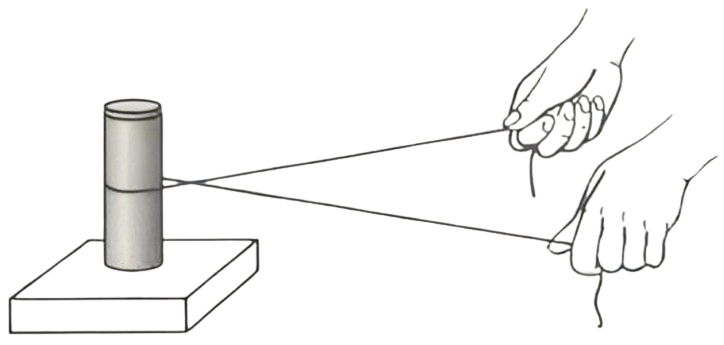
\includegraphics[width=4cm]{Images/coxat}}
	\choiceTF[t]
	{\True Có sự chuyển hóa từ cơ năng sang nhiệt năng khi kéo đi kéo lại sợi dây}
	{\True Có sự truyền nhiệt năng từ ống nhôm vào nước làm nước nóng lên}
	{\True Có sự chuyển hóa từ nhiệt năng sang cơ năng nên hơi nước làm nút bật ra}
	{\True Có sự truyền nhiệt năng từ hơi nước ra môi trường bên ngoài và làm hơi nước lạnh đi ngưng tụ thành giọt nước}
	\loigiai{
		\begin{itemchoice}
			\itemch 
			\itemch 
			\itemch 
			\itemch 
		\end{itemchoice}
	}
	\haidong{10}\end{ex}

\begin{ex} \nguon{1}
	Điểm khác nhau giữa sự sôi và sự bay hơi là
	\choiceTF[t]
	{sự sôi chỉ xảy ra trong lòng chất lỏng; sự bay hơi chỉ xảy ra trên bề mặt chất lỏng}
	{sự sôi xảy ra cả bên trong và trên bề mặt chất lỏng; sự bay hơi chỉ xảy ra trong lòng chất lỏng}
	{\True sự sôi xảy ra cả bên trong và trên bề mặt chất lỏng; sự bay hơi chỉ xảy ra trên bề mặt chất lỏng}
	{\True sự sôi xảy ra ở nhiệt độ sôi của chất lỏng; sự bay hơi xảy ra ở mọi nhiệt độ}
	\loigiai{
		\begin{itemchoice}
			\itemch Sự sôi xảy ra ở cả bề mặt lẫn bên trong chất lỏng.
			\itemch Sự bay hơi chỉ xảy ra ở bề mặt của chất lỏng, không phải trong lòng chất lỏng.
			\itemch Sự sôi xảy ra ở cả bên trong và trên bề mặt chất lỏng; sự bay hơi chỉ xảy ra trên bề mặt chất lỏng.
			\itemch Sự sôi xảy ra ở nhiệt độ sôi của chất lỏng; sự bay hơi xảy ra ở mọi nhiệt độ.
		\end{itemchoice}
	}
\end{ex}


\begin{ex}
	Khi nói về sự nóng chảy thì
	\choiceTF[t]
	{\True nhiệt độ nóng chảy của chì là $327^\circ C$, đây cũng là nhiệt độ đông đặc của chì}
	{\True khi nung nóng một thanh chocolate thì thanh mềm dần cho đến khi trở thành chất lỏng, trong quá trình này nhiệt độ của nó tăng liên tục}
	{hàn điện, luyện kim là một trong những ứng dụng của sự bay hơi}
	{nhựa đường là một chất rắn kết tinh vì có cấu trúc tinh thể}
	
	\loigiai{
		\begin{itemchoice}
			\itemch 
			\itemch Nung nóng thanh chocolate thì thanh mềm dần cho đến khi trở thành chất lỏng, trong quá trình này nhiệt độ của nó tăng liên tục. 
			\itemch Hàn điện, luyện kim là một trong những ứng dụng của sự nóng chảy.
			\itemch Nhựa đường là một chất rắn vô định hình vì không có cấu trúc tinh thể.
		\end{itemchoice}
	}
	\haidong{8}\end{ex}


\begin{ex} \nguon{4}
	Chất rắn kết tinh là chất rắn có cấu trúc mạng tinh thể xác định, ngược lại chất rắn vô định hình không có cấu trúc mạng tinh thể xác định. Điều này dẫn đến một số điểm khác nhau về tính chất giữa chúng.
	\choiceTF[t]
	{\True Chất rắn kết tinh có nhiệt độ nóng chảy xác định, chất rắn vô định hình không có nhiệt độ nóng chảy xác định}
	{Chất rắn kết tinh có cấu trúc mạng tinh thể nên cứng hơn chất rắn vô định hình}
	{Các phân tử trong chất rắn vô định hình không có lực tương tác với nhau nên chất rắn vô định hình không có hình dạng xác định}
	{Khi ta đập vỡ một chất rắn kết tinh thành các mảnh vụn, các mảnh vụn này sẽ không còn cấu trúc mạng tinh thể}
	\loigiai{
		\begin{itemchoice}
			\itemch 
			\itemch Không thể nói chất rắn kết tinh cứng hơn chất rắn vô định hình dựa vào cấu trúc mạng tinh thể.
			\itemch Các phân tử trong chất rắn vô định hình vẫn có lực tương tác với nhau.
			\itemch Khi bị vỡ vụn, các mảnh vỡ của chất rắn kết tinh vẫn có hình dạng xác định vì nó vẫn còn giữ được cấu trúc mạng tinh thể.
		\end{itemchoice}
	}
\end{ex}
\begin{ex}
	Bạn An lấy một viên đá lạnh nhỏ ở trong tủ lạnh rồi bỏ lên chiếc đĩa. Khoảng một giờ sau, bạn An không thấy viên đá lạnh đâu nữa mà thấy nước trải đều trên mặt đĩa. Bạn An để luôn vậy và ra làm rau cùng mẹ. Đến trưa, bạn đến lấy chiếc đĩa ra để rửa thì không còn thấy nước.
	\choiceTF[t]
	{Nước chỉ tồn tại ở thể rắn}
	{\True Nước loang đều trên mặt đĩa vì các phân tử nước liên kết với nhau không mạnh như thể rắn nên nó trượt đều ra}
	{\True Nước đã bay hơi nên không còn trên đĩa nữa}
	{Nếu để một cốc có chứa đá lạnh bên trong, sau một thời gian thấy có nước ở bên ngoài cốc là do nước từ trong cốc chui ra ngoài}
	
	\loigiai{
		\begin{itemchoice}
			\itemch vì nước tồn tại ở cả 3 thể: rắn, lỏng, khí
			\itemch 
			\itemch 
			\itemch vì do đá lạnh nên môi trường xung quanh cốc lạnh hơn làm hơi nước trong không khí ngưng tụ thành nước lỏng mà ta nhìn thấy
		\end{itemchoice}
	}
	\haidong{9}\end{ex}
\begin{ex}
	\immini[thm]{Trong thí nghiệm đun nóng một chất, một học sinh thu được đồ thị sự thay đổi của nhiệt độ theo thời gian như hình.
		\begin{enumerate}[label=\alph*)]
			\item Tại các thời điểm $A,\ B,\ C$ và $D$, chất đó ở thể gì?
			\item Nhiệt độ nóng chảy của chất đó là bao nhiêu?
			\item Nhiệt độ sôi của chất đó là bao nhiêu?
			\item Nhiệt độ thay đổi như thế nào trong quá trình diễn ra sự chuyển thể?
			\item Chất đó có phải là nước tinh khiết không? Vì sao?
	\end{enumerate}}{\begin{tikzpicture}[scale=0.8,transform shape,thick,>=stealth']
			\tkzDefPoints{0/0/o,7/0/x, 0/5/y}
			\tkzDrawSegments[->](o,x o,y)
			\tkzLabelPoint[below left](o){$0$}
			\node at (3,-1) {};
			\node[rotate=90] at (-1,2.5) {Nhiệt độ ($^\circ C$) };
			\node at (3,-0.5) {Thời gian};
			\draw[dashed,thin] (0,1.25) -- (1,1.25);
			\draw[dashed,thin] (0,3.25) -- (4.25,3.25);
			\draw[very thick,red]  plot[smooth, tension=.7] coordinates {(0,0) (0.3,0.65) (0.575,1.1) (0.875,1.25)};
			\draw[very thick,red] (0.875,1.25) -- (2.75,1.25);
			\draw [very thick,red] plot[smooth, tension=.7] coordinates {(2.75,1.25) (3.25,1.4) (3.5,2) (3.75,3) (4,3.25)};
			\draw [very thick,red](4,3.25) -- (6,3.25);
			\draw[very thick,red] plot[smooth, tension=.7] coordinates {(5.975,3.25) (6.325,3.525) (6.65,4.75)};
			\node[left] at (0,1.25) {$17$};
			\node[left] at (0,3.25) {$115$};
			\tkzDefPoints{0.375/0.75/a, 1.75/1.25/b, 5/3.25/d, 3.575/2.25/c}
			\tkzDrawPoints[size=4,fill=white](a,b,c,d)
			\tkzLabelPoint[below right](a){$A$}
			\tkzLabelPoint[above](b){$B$}
			\tkzLabelPoint[right](c){$C$}
			\tkzLabelPoint[above](d){$D$}
	\end{tikzpicture}}
	\loigiai{
		\begin{itemize}
			\item Quan sát đồ thị ta thấy: đồ thị xuất phát ở gốc toạ độ và nhìn chung, nhiệt độ tăng theo thời gian. Đồ thị có 2 đoạn nằm ngang, ở đó nhiệt độ của chất không đổi. Đoạn đồ thị nằm ngang thứ nhất tương ứng với quá trình chuyển từ thể rắn sang thể lỏng (sự nóng chảy). Đoạn nằm ngang thứ hai tương ứng với quá trình sôi, chất chuyển từ thể lỏng sang thể hơi (sự hoá hơi).
			\item a)
			\begin{itemize}
				\item  Tại thời điểm A: chất ở thể rắn.
				\item  Tại thời điểm $B$: chất ở cả thể rắn lẫn thể lỏng.
				\item  Tại thời điểm C: chất ở thể lỏng.
				\item  Tại thời điểm D: chất ở cả thể lỏng lẫn thể hơi.
			\end{itemize}
			
			\item Nhiệt độ nóng chảy của chất đó là $17^{\circ} C$.
			\item Nhiệt độ sôi của chất đó là $115^{\circ} C$.
			\item d)Nhiệt độ của chất không thay đổi trong quá trình nóng chảy và sôi.
			\item Chất đó không phải là nước tinh khiết vì nhiệt độ nóng chảy của nước tinh khiết là $0^{\circ} C$ và nhiệt độ sôi của nước tinh khiết là $100^{\circ} C$.
		\end{itemize} 
	}
\end{ex}
\section{Nội năng - định luật 1 của nhiệt động lực học}
\subsection{Lí thuyết}
\loai{Loại 1: Thế năng phân tử}


\begin{ex}
	Khi dùng pit-tông nén khí trong một xilanh kín thì
	\choice
	{kích thước mỗi phân tử khí giảm}
	{khối lượng mỗi phân tử khí giảm}
	{\True khoảng cách trung bình giữa các phân tử khí giảm}
	{số phân tử khí giảm}
	\loigiai{
		Khi dùng pit-tông nén khí trong một xilanh kín, thể tích của khí bị giảm đi. Điều này dẫn đến khoảng cách giữa các phân tử khí giảm xuống, làm cho mật độ khí tăng lên. Kích thước và khối lượng của từng phân tử khí không thay đổi, cũng như số lượng phân tử khí vẫn được giữ nguyên trong hệ kín.
	}
	\haidong{2}\end{ex}



\loai{Loại 2: Động năng phân tử}




\loai{Loại 3: Thế năng và động năng phân tử}
\begin{ex}
	Cho các nhận định sau:
	\begin{itemize}
		\item[(1)] Nhiệt độ của vật liên quan đến vận tốc chuyển động của các phân tử, nghĩa là liên quan đến động năng phân tử.
		\item [(2)] Thể tích của vật liên quan đến khoảng cách giữa các phân tử, nghĩa là liên quan đến lực tương tác phân tử và thế năng phân tử.
		\item[] Nhận định nào là đúng?
	\end{itemize}
	\choice
	{Chỉ (1)}
	{Chỉ (2)}
	{\True Cả hai}
	{Không có nhận định nào đúng}
	\loigiai{
		Nhiệt độ của vật biểu hiện mức độ chuyển động nhiệt của các phân tử, do đó nó liên quan đến động năng của các phân tử (nhận định 1 đúng). Thể tích của vật liên quan đến khoảng cách giữa các phân tử và do đó cũng liên quan đến lực tương tác phân tử và thế năng phân tử (nhận định 2 đúng). Cả hai nhận định trên đều chính xác.
	}
	\haidong{4}\end{ex}



\loai{Loại 4: Khái niệm nội năng}





\begin{ex}
	Khi năng lượng của các phân tử cấu tạo nên vật giảm thì
	\choice
	{nội năng của vật tăng}
	{nội năng của vật tăng rồi giảm}
	{\True nội năng của vật cũng giảm}
	{nội năng của vật không thay đổi}
	\loigiai{
		Khi năng lượng của các phân tử cấu tạo nên vật giảm (cả động năng và thế năng), nội năng của vật cũng sẽ giảm vì nội năng là tổng các dạng năng lượng này.
	}
	\haidong{2}\end{ex}

\begin{ex} \nguon{1}
	Một học sinh cho rằng: "Nội năng của vật chỉ phụ thuộc vào nhiệt độ, vì khi nhiệt độ tăng thì các phân tử chuyển động nhanh hơn, làm tăng động năng của chúng." Cách lập luận này có đầy đủ chưa? Vì sao?
	\choice
	{Đúng, vì nội năng chỉ liên quan đến chuyển động của các phân tử trong vật}
	{\True Sai, vì nội năng không chỉ phụ thuộc vào nhiệt độ mà còn phụ thuộc vào thể tích do ảnh hưởng của thế năng phân tử}
	{Đúng, vì khi nhiệt độ không đổi thì nội năng không thể thay đổi}
	{Sai, vì nội năng chỉ phụ thuộc vào thể tích mà không liên quan đến nhiệt độ}
	\loigiai{
		\begin{itemize}
			\item Ta có: Nội năng $=$ Động năng của các phân tử $+$ thế năng phân tử.
			\item Mà động năng thì phụ thuộc nhiệt độ (t tăng $\Leftrightarrow$ v tăng $\Leftrightarrow$ Wđ tăng...);
			\item Còn thế năng phân tử phụ thuộc thể tích (V thay đổi $\Rightarrow$ khoảng cách phân tử thay đổi $\Rightarrow$ thế năng tương tác phân tử thay đổi).
		\end{itemize}
		
	}
\end{ex}




\loai{Loại 5: Khái niệm nội năng. Phát biểu đúng}


\begin{ex} \nguon{4}
	Phát biểu nào sau đây đúng?
	\choice
	{Nội năng của vật bằng 0 khi vật ở trên mặt đất}
	{\True Nội năng có thể chuyển hóa thành các dạng năng lượng khác}
	{Nội năng là nhiệt lượng vật nhận được khi thực hiện công}
	{Một vật lúc nào cũng có nội năng do đó lúc nào cũng có nhiệt lượng}
	\loigiai{
		Nội năng có thể chuyển hóa thành các dạng năng lượng khác như công cơ học hoặc nhiệt năng.
	}
\end{ex}

\loai{Loại 6: Khái niệm nội năng. Phát biểu sai}
\begin{ex}%[1P6B2-1][Loai3]
	Cách nào sau đây \textbf{không} làm thay đổi nội năng của vật?
	\choice
	{Làm lạnh vật}
	{Cọ xát vật lên mặt bàn}
	{\True Đưa vật lên cao}
	{Đốt nóng vật}
	\loigiai{
		Đưa vật lên cao không làm thay đổi nội năng của vật.
	}
	
	\haidong{2}\end{ex}



\begin{ex} \nguon{3}
	Phát biểu nào sau đây về nội năng là \textbf{không} đúng?
	\choice
	{Nội năng là một dạng năng lượng}
	{\True Nội năng là nhiệt lượng}
	{Nội năng của một vật có thể tăng hoặc giảm}
	{Nội năng có thể chuyển hóa thành các dạng năng lượng khác}
	\loigiai{
		\begin{itemize}
			\item Nội năng là một dạng năng lượng nội tại của vật, không phải là nhiệt lượng.
			\item Nội năng của một vật có thể tăng hoặc giảm tùy thuộc vào việc nó nhận nhiệt, thực hiện công, hoặc mất nhiệt.
			\item Nội năng có thể chuyển hóa thành các dạng năng lượng khác như cơ năng hoặc nhiệt năng.
		\end{itemize}
	}
\end{ex}

\begin{ex} \nguon{3}
	Phát biểu nào sau đây là \textbf{sai} khi nói về nội năng?
	\choice
	{Nội năng của một vật là dạng năng lượng bao gồm tổng động năng của các phân tử cấu tạo nên vật và thế năng tương tác giữa chúng}
	{Đơn vị của nội năng là Jun (J)}
	{Nội năng của một vật phụ thuộc vào nhiệt độ và thể tích của vật}
	{\True Nội năng không thể biến đổi được}
	\loigiai{
		\begin{itemize}
			\item Nội năng là dạng năng lượng bao gồm tổng động năng của các phân tử cấu tạo nên vật và thế năng tương tác giữa chúng.
			\item Đơn vị của nội năng là Jun (J).
			\item Nội năng phụ thuộc vào nhiệt độ và thể tích của vật.
			\item Nội năng có thể biến đổi trong các quá trình như thực hiện công hay truyền nhiệt, nên phát biểu "Nội năng không thể biến đổi được" là sai.
		\end{itemize}
	}
\end{ex}


\loai{Loại 7: Nhiệt năng và nội năng}

\begin{ex} \nguon{3}
	Phát biểu nào sau đây nói về nhiệt lượng là \textbf{không} đúng?
	\choice
	{Nhiệt lượng là số đo độ biến thiên nội năng của vật trong quá trình truyền nhiệt}
	{\True Một vật lúc nào cũng có nội năng, do đó lúc nào cũng có nhiệt lượng}
	{Đơn vị nhiệt lượng cũng là đơn vị nội năng}
	{Nhiệt lượng không phải là nội năng}
	\loigiai{
		Chỉ khi nào vật có sự biến thiên nội năng do sự truyền nhiệt thì mới có nhiệt lượng.
	}
\end{ex}


\begin{ex}
	Phát biểu nào sau đây là \textbf{sai}?
	\choice
	{Nội năng là một dạng năng lượng nên có thể chuyển hóa thành các dạng năng lượng khác}
	{Nội năng của một vật phụ thuộc vào nhiệt độ và thể tích của vật}
	{\True Nội năng chính là nhiệt lượng của vật}
	{Nội năng của vật có thể tăng hoặc giảm}
	\loigiai{
		Phát biểu "Nội năng chính là nhiệt lượng của vật" là sai. Nội năng của một vật là tổng của động năng và thế năng của các phân tử cấu tạo nên vật. Nhiệt lượng là phần năng lượng nhiệt mà vật trao đổi với các vật khác.
	}
	\haidong{2}\end{ex}



\begin{ex} \nguon{3}
	Nhiệt năng và nội năng khác nhau ở chỗ
	\choice
	{Nội năng của vật có động năng phân tử còn nhiệt năng thì không}
	{Nhiệt năng của vật có thế năng phân tử còn nội năng thì không}
	{\True Nội năng của vật có thế năng phân tử còn nhiệt năng thì không}
	{Nhiệt năng của vật có động năng phân tử còn nội năng thì không}
	\loigiai{
		\begin{center}
			\begin{tabular}{|l|l|l|}
				\hline
				& \multicolumn{1}{|c|}{Nhiệt năng} & \multicolumn{1}{c|}{Nội năng} \\
				\hline
				Phân biệt & \begin{tabular}{l}
					là tổng động năng \\
					 của các phân tử, nguyên tử\\
					  cấu tạo nên vật. \\
				\end{tabular} & \begin{tabular}{l}
					là tổng động năng và thế năng \\
					của các phân tử, nguyên tử\\
					 cấu tạo nên vật. \\
				\end{tabular} \\
				\hline
			\end{tabular}
		\end{center}
	}
\end{ex}


\loai{Loại 8: Thay đổi nội năng bằng cách thực hiện công}


\begin{ex}
	Cách nào sau đây làm thay đổi nội năng bằng hình thức thực hiện công cơ học?
	\choice
	{Bỏ miếng kim loại vào nước nóng}
	{\True Cọ xát một miếng kim loại trên mặt bàn}
	{Bỏ miếng kim loại vào nước đá}
	{Hơ nóng miếng kim loại trên ngọn lửa đèn cồn}
	\loigiai{
		Cọ xát một miếng kim loại trên mặt bàn là cách làm thay đổi nội năng bằng thực hiện công cơ học. Khi cọ xát, công cơ học được chuyển hóa thành nhiệt năng, làm tăng nội năng của miếng kim loại.
	}
	\haidong{2}\end{ex}



\begin{ex}%[1P6B3-1][Loai4]
	Trường hợp nào dưới đây làm biến đổi nội năng \textbf{không} do thực hiện công?
	\choice
	{Đóng đinh}
	{Khuấy nước}
	{Mài dao}
	{\True Nung sắt trong lò}
	\loigiai{
		\begin{itemize}
			\item[A.] Đây là quá trình thay đổi nội năng chỉ bằng cách thực hiện công. 
			\item[B.] Đây là quá trình thay đổi nội năng của bằng cách thực hiện công.
			\item[C.] Đây là quá trình thay đổi nội năng bằng cách thực hiện công.
			\item[D.] Nung sắt trong lò làm tăng nhiệt độ $\Rightarrow$ biến đổi nội năng mà nguyên nhân chỉ là do truyền nhiệt.
		\end{itemize}
	}%<MyLT1>
	\haidong{1}\end{ex}





\loai{Loại 9: Thay đổi nội năng bằng cách truyền nhiệt}
\begin{ex}
	Sự truyền nhiệt là
	\choice
	{sự chuyển hóa năng lượng từ dạng này sang dạng khác}
	{\True sự truyền trực tiếp nội năng từ vật này sang vật khác}
	{sự chuyển hóa năng lượng từ nội năng sang dạng khác}
	{sự truyền trực tiếp nội năng và chuyển hóa năng lượng từ dạng này sang dạng khác}
	\loigiai{
		Sự truyền nhiệt là quá trình truyền trực tiếp nội năng từ vật này sang vật khác thông qua các phương thức như dẫn nhiệt, đối lưu, hay bức xạ. Trong quá trình này, nội năng của vật nóng truyền sang vật lạnh cho đến khi đạt được trạng thái cân bằng nhiệt.
	}
	\haidong{4}\end{ex}


\begin{ex} \nguon{1}
	Phát biểu nào sau đây đúng?
	\choice
	{Nhiệt lượng là một dạng năng lượng, có đơn vị là Jun}
	{Một vật có nhiệt độ càng cao thì càng chứa nhiều nhiệt lượng}
	{Trong quá trình truyền nhiệt và thực hiện công, nội năng của vật được bảo toàn}
	{\True Trong sự truyền nhiệt không có sự chuyển hóa năng lượng từ dạng này sang dạng khác}
	
	\loigiai{
		\begin{itemize}
			\item Phát biểu đúng là: "Trong sự truyền nhiệt không có sự chuyển hóa năng lượng từ dạng này sang dạng khác".
			
			\item Giải thích chi tiết:
			
			a) Nhiệt lượng là một dạng năng lượng, có đơn vị là Jun: Sai. Nhiệt lượng không phải là một dạng năng lượng mà là quá trình truyền năng lượng nhiệt. Đơn vị của nhiệt lượng là Jun (J).
			
			b) Một vật có nhiệt độ càng cao thì càng chứa nhiều nhiệt lượng: Sai. Nhiệt độ của một vật chỉ là thước đo mức độ chuyển động nhiệt của các phân tử. Tổng năng lượng nhiệt của một vật (gồm nội năng) không chỉ phụ thuộc vào nhiệt độ mà còn phụ thuộc vào khối lượng và nhiệt dung riêng của vật đó.
			
			c) Trong quá trình truyền nhiệt và thực hiện công, nội năng của vật được bảo toàn: Sai. Nếu vừa truyền nhiệt vừa thực hiện công thì nội năng của vật sẽ phải giảm.
			
			d) Trong sự truyền nhiệt không có sự chuyển hóa năng lượng từ dạng này sang dạng khác: Đúng. Trong quá trình truyền nhiệt, năng lượng được trao đổi dưới dạng nhiệt mà không có sự chuyển hóa giữa các dạng năng lượng khác nhau (như cơ năng, hóa năng, ...).
		\end{itemize}
	}
\end{ex}


\loai{Loại 10: Thay đổi nội năng bằng cách truyền nhiệt và thực hiện công}
\begin{ex}
	Phát biểu nào sau đây nói về truyền nhiệt và thực hiện công là \textbf{không} đúng?
	\choice
	{Thực hiện công là quá trình có thể làm thay đổi nội năng của vật}
	{Trong thực hiện công có sự chuyển hoá từ nội năng thành cơ năng và ngược lại}
	{Trong truyền nhiệt có sự truyền động năng từ phân tử này sang phân tử khác}
	{\True Trong truyền nhiệt có sự chuyển hoá từ cơ năng sang nội năng và ngược lại}
	\loigiai{
		Phát biểu "Trong truyền nhiệt có sự chuyển hoá từ cơ năng sang nội năng và ngược lại" là không đúng. Trong truyền nhiệt, các phân tử trao đổi động năng với nhau, không liên quan đến sự chuyển hoá giữa cơ năng và nội năng.
	}
	\haidong{2}\end{ex}
\loai{Loại 12: Biểu thức định luật I}




\begin{ex}
	Định luật I của nhiệt động lực học là vận dụng định luật nào sau đây?
	\choice
	{Định luật bảo toàn động năng}
	{Định luật bảo toàn cơ năng}
	{\True Định luật bảo toàn năng lượng}
	{Định luật bảo toàn động lượng}
	\loigiai{
		Định luật I của nhiệt động lực học là một biểu hiện cụ thể của định luật bảo toàn năng lượng. Nó chỉ ra rằng tổng năng lượng trong một hệ kín (bao gồm nội năng, công và nhiệt) luôn được bảo toàn.
	}
	\haidong{2}\end{ex}

\begin{ex} \nguon{1}
	Khi đun nóng khí trong bình không dãn nở, hệ thức phù hợp là
	\choice
	{\True $\Delta U=Q$ với $Q>0$}
	{$\Delta U=Q+A$ với $A<0,~ Q>0$}
	{$Q+A=0$ với $A>0,~ Q<0$}
	{$\Delta U=Q+A$ với $A>0,~ Q<0$}
	\loigiai{
		\begin{itemize}
			\item Khi đun nóng khí trong bình không dãn nở, thể tích của khí không thay đổi, nghĩa là không có công thực hiện.
			
			\item Do đó, công thức của nguyên lí thứ nhất của nhiệt động lực học trở thành:
			$
			\Delta U = Q
			$
			
			\item Với $Q$ là nhiệt lượng mà hệ nhận được. Khi khí được đun nóng, nhiệt lượng được truyền vào hệ, nên $Q > 0$.
			
			\item Vậy hệ thức phù hợp là:
			$
			\Delta U = Q \text{ với } Q > 0
			$\end{itemize}
	}
\end{ex}
\loai{Loại 13: Dấu của A, Q và Delta U}


\begin{ex} \nguon{1}
	Trong quá trình chất khí nhận nhiệt và sinh công thì công thức $\Delta U=A+Q$ phải thỏa mãn hệ thức nào sau đây?
	\choice
	{$Q<0$ và $A>0$}
	{$Q>0$ và $A>0$}
	{$Q<0$ và $A<0$}
	{\True $Q>0$ và $A<0$}
	\loigiai{
		\begin{itemize}
			\item Theo nguyên lí thứ nhất của nhiệt động lực học, độ biến thiên nội năng $\Delta U$ của hệ được tính theo công thức:
			$
			\Delta U = A + Q
			$
			
			\item  $A$ là công mà hệ nhận được (với $A > 0$ khi công được truyền vào hệ, $A < 0$ khi hệ thực hiện công ra ngoài).
			\item  $Q$ là nhiệt lượng mà hệ nhận được (với $Q > 0$ khi hệ nhận nhiệt, $Q < 0$ khi hệ truyền nhiệt ra ngoài).
			
			\item Trong quá trình chất khí nhận nhiệt và sinh công:
			\item  Chất khí nhận nhiệt, nên $Q > 0$.
			\item  Chất khí thực hiện công ra ngoài, nên $A < 0$.
			
			\item Vậy công thức $\Delta U = A + Q$ phải thỏa mãn $Q > 0$ và $A < 0$.\end{itemize}
	}
\end{ex}

\begin{ex}%[1P6B3-1][Loai2]
	Định luật I của nhiệt động lực học được diễn tả bởi công thức $\Delta U = A + Q$, với quy ước
	\choice
	{$Q < 0$: hệ nhận nhiệt}
	{$A < 0$: hệ nhận công}
	{$Q > 0$: hệ truyền nhiệt}
	{\True $A > 0$: hệ nhận công}
	\loigiai{
		\begin{itemize}
			\item Định luật I của nhiệt động lực học được diễn tả bởi công thức $\Delta U = A + Q$, với quy ước $A > 0$: hệ nhận công.
		\end{itemize}
	}
	
	\haidong{2}\end{ex}


\begin{ex}%[1P6Y3-1][Loai2] 
	Hệ thức $\Delta U = A+Q$ với $A > 0,\ Q < 0$ diễn tả cho quá trình nào của chất khí?
	\choice
	{\True Nhận công và tỏa nhiệt}
	{Nhận nhiệt và sinh công}
	{Tỏa nhiệt và nội năng giảm}
	{Nhận công và nội năng giảm}
	\loigiai{
		\begin{itemize}
			\item Theo quy ước dấu: $A>0$: khí nhận công; $Q<0$: khí tỏa nhiệt.
		\end{itemize}
	}
	
	\haidong{2}\end{ex}

\begin{ex}
	Dùng tay nén pit-tông đồng thời nung nóng khí trong một xilanh. Xác định dấu của $A$ và $Q$.
	\choice
	{\True $A > 0;~Q > 0$}
	{$A < 0;~Q > 0$}
	{$A > 0;~Q < 0$}
	{$A < 0;~Q < 0$}
	\loigiai{
		Khi dùng tay nén pit-tông, công được thực hiện lên khí trong xilanh, do đó $A > 0$. Đồng thời, khí được nung nóng, có nghĩa là nhiệt lượng $Q$ truyền vào hệ, do đó $Q > 0$. Vì thế, trong trường hợp này, cả $A$ và $Q$ đều dương.
	}
	\haidong{2}
\end{ex}

\begin{ex}
	Quy ước dấu nào sau đây phù hợp với định luật I của nhiệt động lực học?
	\choice
	{Vật nhận công: $A < 0$; vật nhận nhiệt lượng: $Q < 0$}
	{\True Vật nhận công: $A > 0$; vật nhận nhiệt lượng: $Q > 0$}
	{Vật thực hiện công: $A > 0$; vật truyền nhiệt lượng: $Q > 0$}
	{Vật thực hiện công: $A > 0$; vật truyền nhiệt lượng: $Q < 0$}
	\loigiai{
		Định luật I của nhiệt động lực học quy ước rằng:
		\begin{itemize}
			\item Công $A$ hệ nhận vào là dương ($A > 0$).
			\item Nhiệt lượng $Q$ hệ nhận vào là dương ($Q > 0$).
		\end{itemize}
		Quy ước dấu này giúp xác định rõ ràng dấu của $A$ và $Q$ khi phân tích từng quá trình nhiệt động lực học. Quy tắc với định luật I của nhiệt động lực học là khi vật nhận công thì $A > 0$ và khi vật nhận nhiệt lượng thì $Q > 0$.
	}
	\haidong{2}
\end{ex}
\loai{Loại 14: Biến thiên nội năng}
\begin{ex}
	Phát biểu nào sau đây \textbf{không} đúng?
	\choice
	{\True Biến thiên nội năng là quá trình thay đổi cơ năng của vật}
	{Biến thiên nội năng là quá trình thay đổi nội năng của vật}
	{Độ biến thiên nội năng $\Delta U$ là phần nội năng tăng thêm hay giảm bớt đi trong một quá trình}
	{Đơn vị của nội năng là Jun (J)}
	\loigiai{
		Biến thiên nội năng là sự thay đổi nội năng của một hệ thống, không phải là sự thay đổi cơ năng. Nội năng bao gồm tổng động năng và thế năng của tất cả các phân tử trong hệ, và sự biến thiên nội năng phản ánh sự thay đổi của các yếu tố này chứ không liên quan trực tiếp đến cơ năng của vật.
	}
	\haidong{2}\end{ex}


\begin{ex}
	Đơn vị của độ biến thiên nội năng $\Delta U$ là
	\choice
	{$^\circ C$}
	{K}
	{\True J}
	{Pa}
	\loigiai{
		Đơn vị của độ biến thiên nội năng ($\Delta U$) trong hệ thống đơn vị quốc tế (SI) là Joule (J). Nhiệt lượng ($Q$) và công ($A$) đều có đơn vị là Joule (J), vì cả ba đại lượng này đều đo lường năng lượng hoặc công.
	}
	\haidong{2}
\end{ex}

\begin{ex}%[1P6B3-1][Loai3] 
	Phát biểu nào sau đây đúng?
	\choice
	{Độ biến thiên nội năng của một vật là độ biến thiên nhiệt độ của vật đó}
	{Nội năng còn gọi là nhiệt lượng}
	{Nội năng là phần năng lượng vật nhận được hay mất đi trong quá trình truyền nhiệt}
	{\True Có thể làm thay đổi nội năng của vật bằng cách thực hiện công}
	\loigiai{
		\begin{itemize}
			\item Có hai cách làm thay đổi nội năng của vật là truyền nhiệt và thực hiện công
		\end{itemize}.
	}
	%<MyLT3>
	\haidong{2}\end{ex}


\begin{ex} \nguon{1}
	Theo định luật I của nhiệt động lực học, độ biến thiên nội năng của vật bằng
	\choice
	{\True tổng đại số của công và nhiệt lượng mà vật nhận được}
	{nhiệt lượng mà vật nhận được}
	{tích của công và nhiệt lượng mà vật nhận được}
	{công mà vật nhận được}
	\loigiai{
		\begin{itemize}
			\item Theo Định luật I của nhiệt động lực học, độ biến thiên nội năng của hệ ($\Delta U$) bằng tổng đại số của nhiệt lượng ($Q$) mà hệ nhận được và công ($A$) mà hệ nhận được:
			$
			\Delta U = Q + A
			$
			
			\item Do đó, phát biểu đúng là "Tổng đại số của công và nhiệt lượng mà vật nhận được".\end{itemize}
	}
\end{ex}





\begin{ex} \nguon{1}
	Phát biểu nào sau đây đúng?
	\choice
	{Nội năng của một hệ nhất định phải có thế năng tương tác giữa các hạt cấu tạo nên hệ}
	{Nhiệt lượng truyền cho hệ chỉ làm tăng tổng động năng của chuyển động nhiệt của các hạt cấu tạo nên hệ}
	{\True Công tác động lên hệ có thể làm thay đổi cả tổng động năng chuyển động nhiệt của các hạt cấu tạo nên hệ và thế năng tương tác giữa chúng}
	{Nếu thể tích của hệ thay đổi thì nội năng của hệ phải thay đổi}
	
	\loigiai{
		\begin{itemize}
			\item Phát biểu đúng là: "Công tác động lên hệ có thể làm thay đổi cả tổng động năng chuyển động nhiệt của các hạt cấu tạo nên hệ và thế năng tương tác giữa chúng".
			\item Giải thích chi tiết:
			\begin{itemize}
				\item[a)] Nội năng của một hệ nhất định phải có thế năng tương tác giữa các hạt cấu tạo nên hệ: Sai. Nội năng của một hệ bao gồm cả động năng và thế năng, nhưng trong một số trường hợp đơn giản, có thể bỏ qua thế năng tương tác giữa các hạt.
				
				\item[b)] Nhiệt lượng truyền cho hệ chỉ làm tăng tổng động năng của chuyển động nhiệt của các hạt cấu tạo nên hệ: Sai. Nhiệt lượng truyền vào hệ có thể làm tăng cả động năng và thế năng.
				
				\item[c)] Công tác động lên hệ có thể làm thay đổi cả tổng động năng chuyển động nhiệt của các hạt cấu tạo nên hệ và thế năng tương tác giữa chúng: Đúng. Công thực hiện lên hệ có thể thay đổi cả động năng (liên quan đến chuyển động nhiệt) và thế năng (liên quan đến tương tác giữa các hạt).
				
				\item[d)] Nếu thể tích của hệ thay đổi thì nội năng của hệ phải thay đổi: Sai. Thể tích thay đổi không nhất thiết kéo theo sự thay đổi của nội năng, vì nội năng còn phụ thuộc vào các yếu tố khác như nhiệt độ và lực tương tác giữa các phân tử.
			\end{itemize}
		\end{itemize}
	}
\end{ex}


\begin{ex} \nguon{4}
	Với cùng một lượng khí trong xilanh có pit-tông bịt kín phía trên. Một học sinh thực hiện hai việc như sau:
	\begin{itemize}
		\item[$\bullet$] Ấn nhanh và mạnh pit-tông từ trên xuống để nén lượng khí trong xilanh.
		\item[$\bullet$] Kéo nhanh và mạnh pit-tông lên phía trên để dãn lượng khí trong xilanh.
	\end{itemize}
	Xem như hệ không trao đổi nhiệt với bên ngoài. Hãy cho biết sự biến đổi nội năng của khối khí trong từng trường hợp.
	\choice
	{Khi nén khí, nội năng giảm; khi dãn khí, nội năng tăng}
	{\True Khi nén khí, nội năng tăng; khi dãn khí, nội năng giảm}
	{Nội năng của khí không thay đổi trong cả hai trường hợp}
	{Cả hai trường hợp đều làm tăng nội năng của khí}
	\loigiai{
		Khi khối khí trong xilanh bị nén, khoảng cách giữa các phân tử giảm xuống, thế năng tương tác tăng. Vì vậy nội năng của khối khí tăng lên.
		Khi khối khí trong xilanh bị giãn khoảng cách giữa các phân tử tăng lên thế năng tương tác giảm. Vì vậy nội năng của khối khí giảm xuống.
	}
\end{ex}

\begin{ex} \nguon{4}
	Một học sinh thực hiện một số việc như sau để làm thay đổi nội năng của một đồng $xu$:
	\begin{itemize}
		\item[$\bullet$] Cọ xát đồng $xu$ xuống sàn nhà.
		\item[$\bullet$] Rót nước nóng vào cốc có chứa một đồng xu ở nhiệt độ phòng.
		\item[$\bullet$] Ném mạnh đồng xu xuống cát.
		\item[$\bullet$] Nung nóng đồng $xu$ trên ngọn lửa.
		\item[$\bullet$] Thả một đồng xu từ trên cao vào cốc nước nóng.
	\end{itemize}
	\choice
	{Cọ xát, ném xuống cát: truyền nhiệt; rót nước nóng, nung trên lửa: thực hiện công}
	{\True Cọ xát, ném xuống cát: thực hiện công; rót nước nóng, nung trên lửa: truyền nhiệt}
	{Cọ xát, rót nước nóng, nung trên lửa: thực hiện công; ném xuống cát: truyền nhiệt}
	{Mọi trường hợp đều làm thay đổi nội năng do cả thực hiện công và truyền nhiệt}
	\loigiai{
		\begin{itemize}
			\item Cọ xát đồng $xu$ xuống sàn nhà và ném mạnh đồng xu xuống cát là quá trình thực hiện công.
			\item Rót nước nóng vào cốc có chứa đồng xu và nung nóng đồng xu là quá trình truyền nhiệt.
			\item Thả đồng xu vào cốc nước nóng là vừa có quá trình thực hiện công và truyền nhiệt (thả đồng xu từ trên cao là thực hiện công).
		\end{itemize}
	}
\end{ex}


\loai{Loại 15: Khối khí thực hiện công}
\begin{ex} \nguon{1}
	Khí thực hiện công trong quá trình nào sau đây?
	\choice
	{\True Nhiệt lượng khí nhận được lớn hơn độ tăng nội năng của khí}
	{Nhiệt lượng khí nhận được nhỏ hơn độ tăng nội năng của khí}
	{Nhiệt lượng khí nhận được bằng độ tăng nội năng của khí}
	{Nhiệt lượng khí nhận được lớn hơn hoặc bằng độ tăng nội năng của khí}
	\loigiai{
		\begin{itemize}
			\item Theo Định luật I của nhiệt động lực học:
			$
			\Delta U = Q + A
			$
			\item  $\Delta U$ là độ biến thiên nội năng của khí.
			\item  $Q$ là nhiệt lượng mà khí nhận được (với $Q > 0$ khi khí nhận nhiệt).
			\item  $A$ là công mà khí nhận được.
			
			\item Khi khí thực hiện công, nghĩa là $A < 0$. Do đó, để khí có thể thực hiện công, nhiệt lượng khí nhận được phải lớn hơn độ tăng nội năng của khí. Điều này nghĩa là $Q > \Delta U$.
			
			\item Vì vậy, khí thực hiện công trong quá trình khi nhiệt lượng khí nhận được lớn hơn độ tăng nội năng của khí.\end{itemize}
	}
\end{ex}
\begin{ex}%[1P6B3-1][Loai4]
	Một khối khí thực hiện công trong quá trình nào sau đây?
	\choice
	{\True Nhiệt lượng mà khí nhận được lớn hơn độ tăng nội năng của khí}
	{Nhiệt lượng mà khí nhận được nhỏ hơn độ tăng nội năng của khí}
	{Nhiệt lượng mà khí nhận được bằng độ tăng nội năng của khí}
	{Nhiệt lượng mà khí nhận được có thể lớn hơn hoặc nhỏ hơn nhưng không thể bằng độ tăng nội năng của khí}
	\loigiai{
		\begin{itemize} 
			\item Từ biểu thức định luật I: $\Delta U =A+Q \Rightarrow A=\Delta U -Q$.
			\item Khi nhiệt lượng mà khí nhận được lớn hơn độ tăng nội năng của khí thì $A<0\ \Rightarrow$ khí thực hiện công.
		\end{itemize}
	}
	\haidong{3}\end{ex}
\loai{Loại 16: Động cơ nhiệt}


\begin{ex} \nguon{1}
	Hiệu suất của động cơ nhiệt cho biết
	\choice
	{động cơ thực hiện công nhanh hay chậm}
	{động cơ mạnh hay yếu}
	{\True có bao nhiêu phần trăm nhiệt lượng do nhiên liệu bị đốt cháy tỏa ra được biến đổi thành công có ích}
	{nhiệt lượng tỏa ra khi $1 \ kg$ nhiên liệu bị đốt cháy hoàn toàn trong động cơ}
	\loigiai{
		\begin{itemize}
			\item Hiệu suất của động cơ nhiệt cho biết có bao nhiêu phần trăm nhiệt lượng do nhiên liệu bị đốt cháy tỏa ra được biến đổi thành công có ích. Hiệu suất được tính bằng tỉ số giữa công có ích và nhiệt lượng cung cấp cho động cơ.
			
			\item Do đó, đáp án đúng là "có bao nhiêu phần trăm nhiệt lượng do nhiên liệu bị đốt cháy tỏa ra được biến đổi thành công có ích".\end{itemize}
	}
\end{ex}

\begin{ex} \nguon{1}
	Động cơ nhiệt có thể gây ra tác hại nào đối với môi trường sống của chúng ta?
	\choice
	{Ô nhiễm môi trường do khí thải của các động cơ có nhiều chất độc}
	{Ô nhiễm về tiếng ồn}
	{Góp phần làm tăng nhiệt độ của khí quyển}
	{\True Cả $A,\ B$ và $C$}
	\loigiai{
		\begin{itemize}
			\item Động cơ nhiệt có thể gây ra các tác hại đối với môi trường sống của chúng ta như:
			\item  Ô nhiễm môi trường do khí thải của các động cơ có nhiều chất độc, chẳng hạn như CO, $CO_2$, $NO_x$, và các hạt bụi mịn.
			\item  Ô nhiễm về tiếng ồn do hoạt động của các động cơ.
			\item  Góp phần làm tăng nhiệt độ của khí quyển do hiệu ứng nhà kính từ khí thải $CO_2$ và các chất khác.
			
			\item Do đó, đáp án đúng là "Cả A, B và C".\end{itemize}
	}
\end{ex}



\begin{ex} \nguon{1}
	Kĩ thuật và vật liệu cải tiến có thể được sử dụng trong động cơ nhiệt nhằm giảm sự truyền nhiệt ra môi trường. 
	\choice
	{Chúng có thể hoàn toàn loại bỏ sự truyền nhiệt ra môi trường, giúp động cơ hoạt động với hiệu suất 100\%}
	{\True Chúng có thể giảm đáng kể sự truyền nhiệt ra môi trường, nhưng không thể loại bỏ hoàn toàn sự mất mát nhiệt}
	{Chúng không có tác dụng trong việc giảm sự truyền nhiệt ra môi trường}
	{Chúng có thể chuyển toàn bộ nhiệt lượng nhận được thành công hữu ích}
	\loigiai{
		\begin{itemize}
			\item Kĩ thuật và vật liệu cải tiến có thể làm giảm sự truyền nhiệt ra môi trường, nhưng chúng không thể loại bỏ hoàn toàn sự truyền nhiệt này. \item Bởi vì không thể có một động cơ nào hoạt động được theo cách toàn bộ nhiệt lượng nhận được chuyển hoàn toàn thành công có ích mà không mất mát nhiệt lượng do hao phí.\end{itemize}
	}
\end{ex}

\begin{ex} \nguon{1}
	Yếu tố nào sau đây làm giảm hiệu suất của một động cơ nhiệt?
	\choice
	{Sự thất thoát năng lượng do ma sát và độ nhớt trong động cơ}
	{Quá trình đốt cháy nhiên liệu không hoàn toàn}
	{Một phần nhiệt lượng bị truyền ra môi trường mà không được chuyển hóa thành công cơ học}
	{\True Cả ba yếu tố trên}
	\loigiai{
		Sự thất thoát năng lượng do ma sát, độ nhớt trong động cơ và quá trình đốt cháy không đủ sẽ làm giảm hiệu suất của động cơ nhiệt.
	}
\end{ex}


\begin{ex} \nguon{1}
	Trong công thức tính hiệu suất của động cơ nhiệt, A là
	\choice
	{\True công có ích}
	{nhiệt lượng toả ra của nhiên liệu bị đốt cháy}
	{nhiệt lượng tỏa ra môi trường}
	{nhiệt năng của nhiên liệu}
	\loigiai{
		\begin{itemize}
			\item Trong công thức tính hiệu suất của động cơ nhiệt, A là công có ích mà động cơ thực hiện. Đây là phần năng lượng được chuyển đổi thành công cơ học để làm công việc bên ngoài.
			
			\item Do đó, biểu thức đúng là "công có ích".\end{itemize}
	}
\end{ex}

\begin{ex} \nguon{1}
	Hiện nay hiệu suất của động cơ nhiệt thường có giá trị khoảng
	\choice
	{$100 \%$}
	{\True từ $30 \%$ đến $50 \%$}
	{từ $80 \%$ đến $90 \%$}
	{trên $90 \%$}
	\loigiai{
		\begin{itemize}
			\item Trong thực tế, hiệu suất của động cơ nhiệt thường có giá trị khoảng từ 30\% đến 40\%. 
			\item Phần lớn năng lượng từ nhiên liệu bị mất dưới dạng nhiệt thải và các hình thức tổn thất khác.
			
			\item Do đó, đáp án đúng là "từ 30\% đến 40\%".\end{itemize}
	}
\end{ex}





\loai{Loại 17: Giải thích hiện tượng}
\begin{ex}
	\immini[thm]{Giữ quả bóng bàn bị móp trong tay và dùng máy sấy tóc để hơ nóng quả bóng. Giữ 1-2 phút để làm nóng không khí bên trong quả bóng. Trong hầu hết các trường hợp, vết lõm sẽ bật ra ngay lập tức. Điều này là do }{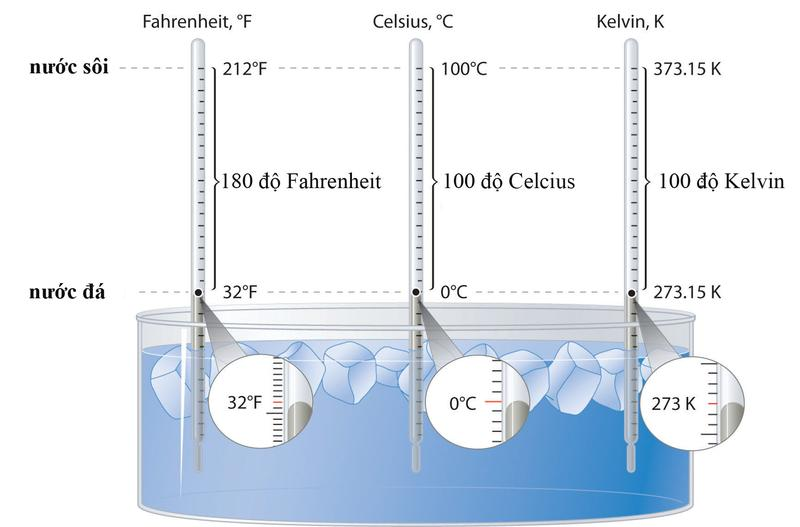
\includegraphics[width=4cm]{Images/bongban}}  
	\choice
	{\True nội năng của không khí bên trong quả bóng tăng lên}
	{nội năng của không khí bên trong quả bóng giảm xuống}
	{nội năng của không khí bên trong quả bóng không thay đổi}
	{nội năng của không khí bên trong quả bóng bị mất đi}  
	\loigiai{
		Khi hơ nóng quả bóng bàn bằng máy sấy, nhiệt lượng từ máy sấy truyền vào không khí bên trong quả bóng làm tăng nhiệt độ của không khí. Sự gia tăng nhiệt độ này làm tăng áp suất bên trong quả bóng, đẩy bề mặt quả bóng ra và làm vết lõm bật ra. Như vậy, nội năng của không khí bên trong quả bóng đã tăng lên nhờ quá trình truyền nhiệt từ máy sấy.
	}
	\haidong{4}\end{ex}







\begin{ex} \nguon{1}
	\immini[thm]{Khi sử dụng bơm tay để bơm xe đạp, thân bơm nóng lên. Nguyên nhân nào sau đây giải thích đúng nhất hiện tượng này?
		\choice
		{Không khí trong bơm nóng lên do tiếp xúc với thân bơm}
		{\True Nhiệt độ của không khí tăng do bị nén và do ma sát giữa pit-tông và thân bơm}
		{Bơm xe làm động năng của không khí trong bơm tăng lên}
		{Không khí trong bơm nóng lên do hút nhiệt từ bên ngoài}	
	}
	{
\includegraphics[width=2cm]{images/bomxe}}
	\loigiai{
		Nguyên nhân là do thực hiện công, pít-tông dịch chuyển trong thân bơm cọ xát lên thân bơm và do khí bị nén trong thân bơm làm nội năng của nó tăng lên.
	}
\end{ex}

\begin{ex} \nguon{4}
	\immini[thm]{Quan sát thí nghiệm hơ nóng một ống nghiệm chứa không khí với nút đậy kín trên ngọn lửa đèn cồn, sau một thời gian chiếc nút bị bật khỏi ống nghiệm. Nguyên nhân nào sau đây giải thích đúng nhất hiện tượng này?
		\choice
		{Không khí trong ống nghiệm bị phân hủy thành các chất khác}
		{\True Nhiệt độ tăng làm tăng động năng của các phân tử khí, dẫn đến áp suất trong ống nghiệm tăng}
		{Nhiệt độ cao làm giảm khối lượng riêng của không khí, khiến nó đẩy nút ra}
		{Không khí trong ống nghiệm bị giãn nở do hấp thụ nhiệt, nhưng không ảnh hưởng đến áp suất}
	}
	{
\includegraphics[width=2cm]{images/nutbac}}
	\loigiai{
		Trong thí nghiệm trên, nội năng thay đổi là do động năng của các phân tử thay đổi vì khi bị nung nóng các phân tử chuyển động nhiệt nhanh hơn. Thế năng tương tác trung bình của các phân tử có thể xem như không đổi vì thể tích khối khí trong quá trình nung nóng là không đổi.
	}
\end{ex}

\begin{ex} \nguon{4}
	Một học sinh cho rằng: “Khi một vật có nội năng lớn tiếp xúc với một vật có nội năng nhỏ hơn thì chắc chắn xảy ra quá trình truyền nhiệt”. Kết luận đúng hay sai?
	\choice
	{Đúng, vì vật có nội năng lớn hơn luôn truyền nhiệt cho vật có nội năng nhỏ hơn}
	{Đúng, vì nội năng quyết định khả năng truyền nhiệt giữa hai vật}
	{\True Sai, vì quá trình truyền nhiệt chỉ xảy ra khi có sự chênh lệch nhiệt độ giữa hai vật}
	{Sai, vì vật có nội năng nhỏ hơn luôn truyền nhiệt cho vật có nội năng lớn hơn}
	\loigiai{
		Kết luận trên là không đúng. Để xảy ra quá trình truyền nhiệt phải có sự chênh lệch nhiệt độ giữa hai vật. Mặc dù hai vật có sự chênh lệch về nội năng nhưng không thể kết luận chắc chắn rằng hai vật có sự chênh lệch về nhiệt độ.
	}
\end{ex}





\begin{ex} \nguon{4}
	\immini[thm]{Ý nghĩa thí nghiệm của Joule là
		\choice
		{\True tìm ra mối quan hệ tương đương giữa công và nhiệt lượng}
		{chứng minh định luật bảo toàn và chuyển hóa năng lượng}
		{chứng minh có sự biến đổi của công thành nội năng}
		{tìm ra nguyên lí thứ nhất của nhiệt động lực học}}{
\includegraphics[width=3.5cm]{images/Joule}}
	\loigiai{
		Thí nghiệm của Jun tìm ra mối quan hệ tương đương giữa công và nhiệt lượng, chứng minh rằng công có thể chuyển hóa thành nhiệt năng.
	}
\end{ex}

\begin{ex} \nguon{4}
	Phát biểu nào sau đây là \textbf{sai}?
	\choice
	{Trong quá trình thực hiện công có sự chuyển hóa từ một dạng năng lượng khác sang nội năng}
	{Quá trình truyền nhiệt là quá trình làm thay đổi nội năng không có sự thực hiện công}
	{Trong quá trình truyền nhiệt chỉ có sự truyền nội năng từ vật này sang vật khác}
	{\True Trong quá trình thực hiện công chỉ có sự chuyển hóa từ động năng sang nội năng}
	\loigiai{
		Trong quá trình thực hiện công, có thể có sự chuyển hóa từ nhiều dạng năng lượng khác (như thế năng, cơ năng) sang nội năng, không chỉ từ động năng.
	}
\end{ex}

\begin{ex} \nguon{4}
	Khi bỏ một miếng đồng vào một cốc nước, một khoảng thời gian sau ta thấy nước trong cốc lạnh hơn so với ban đầu (bỏ qua sự trao đổi nhiệt với môi truờng). Kết luận nào sau đây đúng?
	\choice
	{Khối lượng của nước trong cốc lớn hơn khối lượng của miếng đồng}
	{Đã có sự truyền nhiệt lượng từ miếng đồng sang nước trong cốc}
	{\True Nhiệt độ của miếng đồng tăng lên so với ban đầu}
	{Nội năng của miếng đồng đã giảm xuống}
	\loigiai{
		Nhiệt độ của miếng đồng tăng lên so với ban đầu.
	}
\end{ex}

\loai{Loại 18: Câu hỏi đúng sai}
\begin{ex}
	Khi nói về nhiệt lượng của vật thì
	\choiceTF[t]
	{\True nhiệt lượng là số đo độ tăng nội năng của vật trong quá trình truyền nhiệt}
	{một vật lúc nào cũng có nội năng, do đó lúc nào cũng có nhiệt lượng}
	{\True đơn vị của nhiệt lượng cũng là đơn vị của nội năng}
	{nhiệt lượng của vật chính là nội năng của nó}
	
	\loigiai{
		\begin{itemchoice}
			\itemch 
			\itemch SAI. Nhiệt lượng chỉ có khi có sự truyền nhiệt.
			\itemch 
			\itemch 	SAI. Nhiện lượng là phần nội năng biến thiên trong quá trình truyền nhiệt
		\end{itemchoice}
	}
	\haidong{6}\end{ex}

\begin{ex}
	Khi nói về nội năng của vật thì
	\choiceTF[t]
	{nội năng là tổng động năng của các phân tử cấu tạo nên hệ}
	{\True nội năng của hệ phụ thuộc vào nhiệt độ $T$ và thể tích $V$ của hệ}
	{\True quá trình thực hiện công làm thay đổi nội năng của hệ có sự chuyển hoá năng lượng từ cơ năng sang nội năng}
	{\True quá trình truyền nhiệt làm thay đổi nội năng của hệ chỉ có sự truyền nội năng từ vật này sang vật khác mà không có sự chuyển hoá năng lượng từ dạng này sang dạng khác}
	\loigiai{
		\begin{itemchoice}
			\itemch SAI. Nội năng là tổng động năng và thế năng tương tác của các phân tử cấu tạo nên vật.
			\itemch  ĐÚNG
			\itemch ĐÚNG. Quá trình thực hiện công làm thay đổi nội năng của hệ có sự chuyển hoá năng lượng từ cơ năng sang nội năng.
			\itemch ĐÚNG
		\end{itemchoice}
	}
	\haidong{6}\end{ex}

\begin{ex} \nguon{1}
	Nội năng của một hệ
	\choiceTF[t]
	{là tổng động năng của các phân tử cấu tạo nên vật}
	{\True phụ thuộc vào nhiệt độ của hệ}
	{\True phụ thuộc vào thể tích của hệ}
	{là nhiệt lượng vật nhận được trong quá trình truyền nhiệt}
	\loigiai{
		\begin{itemchoice}
			\itemch Sai. Nội năng không chỉ là tổng động năng của các phân tử cấu tạo nên vật, mà còn bao gồm cả thế năng tương tác giữa các phân tử.
			\itemch Đúng. Nội năng phụ thuộc vào nhiệt độ của hệ, vì nhiệt độ ảnh hưởng đến động năng của các phân tử trong hệ.
			\itemch Đúng. Nội năng phụ thuộc vào thể tích của hệ vì khi thể tích thay đổi, khoảng cách giữa các phân tử thay đổi, ảnh hưởng đến thế năng tương tác giữa chúng.
			\itemch Sai. Nội năng không phải là nhiệt lượng mà vật nhận được. Nhiệt lượng chỉ là một quá trình truyền năng lượng vào hoặc ra khỏi hệ, ảnh hưởng đến sự thay đổi nội năng.
		\end{itemchoice}
	}
\end{ex}

\begin{ex} \nguon{1}
	Nội năng
	\choiceTF[t]
	{\True là một dạng năng lượng}
	{\True có thể chuyển hóa thành các dạng năng lượng khác}
	{là nhiệt lượng}
	{của vật $A$ lớn hơn nội năng của vật $B$ thì nhiệt độ của vật $A$ cũng lớn hơn nhiệt độ của vật $B$}
	\loigiai{
		\begin{itemchoice}
			\itemch Đúng. Nội năng là một dạng năng lượng bên trong của hệ, bao gồm tổng động năng và thế năng của các phân tử cấu tạo nên vật.
			\itemch Đúng. Nội năng có thể chuyển hóa thành các dạng năng lượng khác, chẳng hạn như cơ năng, hóa năng, điện năng, trong quá trình truyền nhiệt hoặc thực hiện công.
			\itemch Sai. Nội năng không phải là nhiệt lượng. Nhiệt lượng là lượng năng lượng trao đổi giữa các hệ do chênh lệch nhiệt độ, còn nội năng là tổng năng lượng bên trong của một hệ.
			\itemch Sai. Nội năng không chỉ phụ thuộc vào nhiệt độ mà còn phụ thuộc vào khối lượng và nhiệt dung riêng của vật. Một vật có nội năng lớn hơn không nhất thiết phải có nhiệt độ cao hơn nếu có khối lượng hoặc nhiệt dung riêng lớn hơn.
		\end{itemchoice}
	}
\end{ex}

\begin{ex} \nguon{1}
	Sự liên quan giữa quá trình chuyển thể của chất và nội năng của vật.
	\choiceTF[t]
	{Vật rắn đang nóng chảy thì nội năng của nó giảm}
	{\True Nước đá đang tan thì nội năng của nó tăng}
	{\True Hơi nước ngưng tụ ở nhiệt độ không đổi thì nội năng của nó giảm}
	{\True Vật trượt trên mặt phẳng nằm nghiêng có ma sát thì nội năng của nó tăng}
	\loigiai{
		\begin{itemchoice}
			\itemch Sai. Khi vật rắn đang nóng chảy, nội năng của nó tăng do cần nhiệt lượng để các phân tử chuyển từ trạng thái rắn sang trạng thái lỏng, mặc dù nhiệt độ không đổi.
			\itemch Đúng. Khi nước đá đang tan, nội năng của nó tăng vì cần hấp thụ nhiệt lượng để phá vỡ liên kết giữa các phân tử trong cấu trúc rắn của nước đá để chuyển thành nước lỏng.
			\itemch Đúng. Khi hơi nước ngưng tụ ở nhiệt độ không đổi, nội năng của nó giảm vì nhiệt lượng được tỏa ra trong quá trình chuyển từ trạng thái khí sang trạng thái lỏng.
			\itemch Đúng. Khi vật trượt trên mặt phẳng nằm nghiêng có ma sát, ma sát làm tăng nhiệt độ của vật và mặt phẳng, do đó tăng nội năng của vật.
		\end{itemchoice}
	}
\end{ex}

\begin{ex} \nguon{3}
	Khi nói về nội năng của hệ.
	\choiceTF[t]
	{\True Nội năng của hệ là một dạng năng lượng và có thể thay đổi được}
	{Thực hiện công và truyền nhiệt không làm thay đổi nội năng của hệ}
	{\True Công tác động lên hệ có thể làm thay đổi cả tổng động năng chuyển động nhiệt của các hạt cấu tạo nên hệ và thế năng tương tác giữa chúng}
	{Nói chung, nội năng là hàm của nhiệt độ và thể tích, nên trong mọi trường hợp nếu thể tích của hệ đã thay đổi thì nội năng của hệ phải thay đổi}
	\loigiai{
		\begin{itemchoice}
			\itemch Đúng
			\itemch Sai vì: $\Delta U=A+Q \Rightarrow$ Nếu thực hiện công hay truyền nhiệt sẽ dẫn tới thay đổi nội năng của hệ.
			\itemch Đúng
			\itemch Sai vì: $\Delta U=A+Q \Rightarrow$ có thể thay đổi thể tích nhưng đồng thời truyền nhiệt lượng cho vật sao cho nội năng của hệ không đổi.
		\end{itemchoice}
	}
\end{ex}

\begin{ex} \nguon{3}
	Khi nói về nội năng của hệ.
	\choiceTF[t]
	{\True Hệ đứng yên vẫn có khả năng sinh công do có nội năng}
	{\True Nội năng bao gồm tổng động năng phân tử và thế năng phân tử}
	{Nội năng không phụ thuộc vào nhiệt độ và thể tích của vật}
	{\True Phần nội năng vật nhận được hay mất đi trong quá trình truyền nhiệt gọi là nhiệt lượng} 
	\loigiai{
		\begin{itemchoice}
			\itemch Đúng
			\itemch Đúng
			\itemch Sai vì: Nội năng của vật bao gồm tổng động năng phân tử và thế năng phân tử, nội năng phụ thuộc vào nhiệt độ và thể tích của vật.
			\itemch Đúng
		\end{itemchoice}
	}
	
\end{ex}
\begin{ex} \nguon{4}
	Khi thực hiện quá trình truyền nhiệt cho vật, ta nói rằng vật nhận thêm nhiệt lượng nên nội năng thay đổi, giữa nội năng và nhiệt lượng có một mối liên hệ qua lại với nhau.
	\choiceTF[t]
	{\True Nhiệt lượng là số đo độ biến thiên nội năng của vật trong quá trình truyền nhiệt}
	{\True Đơn vị của nhiệt lượng cũng là đơn vị của nội năng}
	{Một vật lúc nào cũng có nội năng, do đó lúc nào vật cũng có nhiệt lượng}
	{Một vật có nội năng lớn khi cho tiếp xúc với vật khác có nội năng nhỏ hơn thì sẽ xảy ra quá trình truyền nhiệt}
	\loigiai{
		\begin{itemchoice}
			\itemch Đ
			\itemch Đ
			\itemch S. Nhiệt lượng chỉ xuất hiện trong quá trình truyền nhiệt, không có quá trình truyền nhiệt thì không có nhiệt lượng.
			\itemch Sai. Quá trình truyền nhiệt xảy ra khi hai vật có sự chênh lệch về nhiệt độ chứ không phải phụ thuộc vào độ chênh lệch về nội năng.
		\end{itemchoice}
	}
\end{ex}
\begin{ex} \nguon{1}
	Trường hợp nào làm biến đổi nội năng \textbf{không} do thực hiện công.
	\choiceTF[t]
	{\True Đun nóng nước bằng bếp}
	{Một viên bi bằng thép rơi xuống đất mềm}
	{\True Chậu nước để ngoài nắng một lúc nóng lên}
	{Cọ sát hai vật vào nhau}
	\loigiai{
		\begin{itemchoice}
			\itemch Đúng. Đun nóng nước bằng bếp làm nhiệt truyền từ bếp vào nước, làm tăng nội năng của nước, không thông qua thực hiện công.
			\itemch  Sai. Một viên bi bằng thép rơi xuống đất mềm sẽ biến động năng thành nhiệt năng qua lực cản của đất và ma sát, làm thay đổi nội năng.
			\itemch Đúng. Chậu nước để ngoài nắng một lúc nóng lên là do hấp thụ nhiệt từ ánh sáng mặt trời, làm tăng nội năng của nước, không thông qua thực hiện công.
			\itemch Sai. Cọ sát hai vật vào nhau tạo ma sát làm tăng nhiệt độ của cả hai vật, thông qua lực ma sát, đây là thực hiện công lên vật để tăng nội năng.
		\end{itemchoice}
	}
\end{ex}


\begin{ex} \nguon{4}
	\immini[thm]{Một lượng khí được đặt trong một xilanh như hình bên. Khi bật đèn cồn, người ta nhận thấy nhiệt độ khối khí tăng lên và đẩy pit-tông đi lên.
		\choiceTF[t]
		{\True Nội năng của khối khí đã thay đổi nhờ quá trình truyền nhiệt}
		{Độ biến thiên nội năng của khối khí đúng bằng nhiệt lượng mà khối khí nhận được}
		{\True Khi khối khí dãn nở đẩy pit-tông đi lên, ta nói khối khí đã thực hiện công}
		{Công của khối khí khi đẩy pit-tông đi lên đúng bằng nhiệt lượng mà nó nhận được}}{\vspace*{1 cm} 
\includegraphics[width=2.5cm]{images/2024_05_29_ddddee3750d8eb1e627bg-08}}
	\loigiai{
		\begin{itemchoice}
			\itemch Đúng
			\itemch Sai. Vì nhiệt lượng nhận được được một phần làm thay đổi nội năng của khối khí, một phần chuyển thành công làm đẩy pit-tông đi lên.
			\itemch Đúng
			\itemch Sai. Vì nhiệt lượng nhận được được một phần làm thay đổi nội năng của khối khí, một phần chuyển thành công làm đẩy pit-tông đi lên.
		\end{itemchoice}
	}
\end{ex}
\begin{ex} \nguon{1}
	Động cơ nhiệt
	\choiceTF[t]
	{Chuyển công thành nhiệt}
	{\True Nguồn nóng có nhiệt độ $T_1$ cung cấp nhiệt lượng cho động cơ}
	{\True Bộ phận phát động trong đó tác nhân nhận nhiệt từ nguồn nóng, dãn nở sinh công}
	{Nguồn lạnh có nhiệt độ $T_2<T_1$ nhận công do động cơ tác động}
	\loigiai{
		\begin{itemchoice}
			\itemch 
			\itemch 
			\itemch 
			\itemch 
		\end{itemchoice}
	}
\end{ex}



\begin{ex} \nguon{1}
	\immini[thm]{Ban đầu khi đang đóng đinh vào gỗ, mũ đinh có nóng lên nhưng rất ít. Sau đó khi đinh đã đóng chắc vào gỗ rồi (không lún thêm được nữa) ta lại tiếp tục đóng thêm vài nhát búa nữa.}
	{
\includegraphics[width=1.7cm]{images/dinh}}
	\choiceTF[t]
	{\True Ở những lần đóng đinh cuối (khi đinh đã chắc) thì mũ đinh sẽ nóng hơn trước nhiều}
	{\True Ban đầu công do búa thực hiện phần lớn để thắng công cản trở của gỗ lên đinh}
	{\True Khi đinh đóng chắc vào gỗ rồi thì công do búa thực hiện lên đinh sẽ chuyển phần lớn sang nội năng của đinh}
	{Công do búa thực hiện được chia đều cho việc làm nóng đinh và thắng công cản trở của gỗ lên đinh}	
	
	
	\loigiai{
		\begin{itemchoice}
			\itemch 
			\itemch 
			\itemch Bởi vì khi đang đóng đinh vào gỗ, công do búa thực hiện phần lớn để thắng công cản trở của gỗ lên đinh, một phần thì chuyển thành nội năng của đinh. 
			\itemch Nhưng khi đinh đóng chắc vào gỗ rồi thì công do búa thực hiện lên đinh sẽ chuyển phần lớn sang nội năng của đinh.
		\end{itemchoice}
		
	}
\end{ex}
\begin{ex} \nguon{4}
	\immini[thm]{Hình vẽ bên thể hiện hai cách làm thay đổi nội năng của một vật đó là dùng tay cọ xát miếng đồng trên mặt bàn (hình 1) và cho nước sôi vào trong cốc có sẵn miếng đồng ở nhiệt độ phòng (hình 2).}{
\includegraphics[width=4cm]{images/2024_05_29_ddddee3750d8eb1e627bg-13}}
	\choiceTF[t]
	{Hình 1 thể hiện quá trình truyền nhiệt, hình 2 là quá trình thực hiện công}
	{\True Trong quá trình thực hiện công, có sự chuyển hóa năng lượng từ dạng này sang dạng khác}
	{\True Trong quá trình truyền nhiệt, không có sự chuyển hóa năng lượng từ dạng này sang dạng khác}
	{Nội năng của vật luôn tăng khi ta thực hiện quá trình thực hiện công hoặc quá trình truyền nhiệt}
	\loigiai{
		\begin{itemchoice}
			\itemch Sai. Hình 1 là quá trình thực hiện công, hình 2 là quá trình truyền nhiệt.
			\itemch Đúng.
			\itemch Đúng. Trong quá trình truyền nhiệt chỉ có sự truyền nội năng từ vật này sang vật khác.
			\itemch Sai. Nội năng của vật có thể tăng hoặc giảm khi ta thực hiện công hoặc truyền nhiệt.
		\end{itemchoice}
	}
\end{ex}
\subsection{Bài tập}
\section{Nội năng - định luật 1 nhiệt động lực học}
\begin{ex}
	Một lượng khí được truyền \(10 \ \text{kJ}\) nhiệt năng để nóng lên đồng thời bị nén bởi một lực có độ lớn công của lực là \(100 \ \text{kJ}\). Độ biến thiên nội năng của lượng khí là
	\choice
	{$90 \ \text{kJ}$}
	{\True $110 \ \text{kJ}$}
	{$100 \ \text{kJ}$}
	{0}
	\loigiai{
		Theo định luật I của nhiệt động lực học, độ biến thiên nội năng \(\Delta U\) được tính bằng:
		\[ \Delta U = A + Q \]
		Ở đây, \(A = 100 \ \text{kJ}\) là công hệ nhận được (dương), \(Q = 10 \ \text{kJ}\) là nhiệt lượng truyền vào hệ (dương).
		Do đó:
		\[ \Delta U = 100 \ \text{kJ} + 10 \ \text{kJ} = 110 \ \text{kJ} \]
		Vậy độ biến thiên nội năng của lượng khí là \(110 \ \text{kJ}\).
	}
	\haidong{5}
\end{ex}
\begin{ex}%[1P6-3.2B][Loai1] 
	Người ta truyền cho khí trong xi-lanh nhiệt lượng 100 J. Chất khí nở ra thực hiện công 65 J đẩy pít-tông lên. Nội năng của khí biến thiên một lượng là
	\choice
	{15 J}
	{25 J}
	{\True 35 J}
	{45 J}
	\loigiai{\begin{itemize}
			\item Khí nhận nhiệt: $Q=100\ J$.
			\item Khí dãn nở sinh công: $A=-65\ J$.
			\item Độ biến thiên nội năng của khí: $\Delta U=A+Q=35\ J$.
	\end{itemize}}
	\haidong{4}\end{ex}
\begin{ex} \nguon{1}
	Người ta truyền cho khí trong xi-lanh một nhiệt lượng $200 \ J$. Khí nở ra và thực hiện công $140 \ J$ đẩy pit-tông lên. Độ biến thiên nội năng của khí là
	\choice
	{$340 \ J$}
	{$200 \ J$}
	{$170 \ J$}
	{\True $60 \ J$}
	\loigiai{
		\begin{itemize}
			
			\item $
			\Delta U =
			A + Q = -140  + 200  = 60 \ J
			$
		\end{itemize}
	}
\end{ex}
\begin{ex} \nguon{3}
	Người ta truyền cho một lượng khí trong xi-lanh nhiệt lượng $100\ J$. Khí nở ra thực hiện công $70\ J$ đẩy pit-tông dịch chuyển. Độ biến thiên nội năng của khí là
	\choice
	{$20\ J$}
	{\True $30\ J$}
	{$40\ J$}
	{$-30\ J$}
	\loigiai{
		Ta có $: \left\{\begin{array}{l}Q=100\ J \\ A=-70\ J \end{array}\right. \Rightarrow \Delta U=A+Q=-70+100=30\ J $
	}
\end{ex}
\begin{ex}%[1P6-3.2B][Loai1] 
	Người ta thực hiện một công 200 J để nén khí trong một xi-lanh. Biết khí truyền ra môi trường xung quanh một nhiệt lượng 25 J. Độ biến thiên nội năng của khối khí là
	\choice
	{100 J}
	{125 J}
	{225 J}
	{\True 175 J}
	\loigiai{\begin{itemize}
			\item Thực hiện công lên khối khí suy ra khí nhận công: $A=200\ J$.
			\item Khí truyền nhiệt: $Q=-25\ J$.
			\item Độ biến thiên nội năng của khí: $\Delta U=A+Q=175\ J$.
	\end{itemize}}
	\haidong{5}\end{ex}
\begin{ex}
	Một lượng khí bị nén đã nhận được công là $150 \ kJ$. Khí nóng lên và đã toả nhiệt lượng là 95 kJ ra môi trường. Độ biến thiên nội năng của lượng khí là
	\choice
	{$150 \ kJ$}
	{\True $55 \ kJ$}
	{$245 \ kJ$}
	{0}
	\loigiai{
		Độ biến thiên nội năng: $\Delta U=A+Q=150-95=55\ kJ$.
	}
	\haidong{5}\end{ex}
\begin{ex} \nguon{4}
	Một khối không khí khi nhận được một công $200 \ J$ thì nội năng của nó tăng thêm $120 \ J$. Khi đó khối không khí này
	\choice
	{\True tỏa nhiệt 80 J}
	{nhận nhiệt 80 J}
	{tỏa nhiệt 40 J}
	{nhận nhiệt 40 J}
	%Hãy cho biết sự trao đổi nhiệt lượng giữa khối khí và môi trường diễn ra như thế nào?
	\loigiai{
		\begin{itemize}
			\item Khí nhận công và nội năng tăng nên: $A>0, \Delta U>0$.
			\item Ta có: $\Delta U=Q+A \Rightarrow Q=\Delta U-A=120-200=-80 \ J$.
			\item Vì $Q<0$ nên khối khí đã truyền ra môi trường nhiệt lượng $80 \ J$.
		\end{itemize}
	}
\end{ex}
\begin{ex}
	\immini[thm]{
		Khi truyền nhiệt lượng $6.10^{6}\ J$ cho khí trong một xi-lanh hình trụ thì khí nở ra đẩy pit-tông chuyển động và làm thể tích của khí tăng thêm $0,50\ m^3$. Biết áp suất của khí trong xi-lanh là $8.10^{6}\ N/m^2$ và coi áp suất này không đổi trong quá trình khí thực hiện công. Độ biến thiên nội năng của khí là
		\choice
		{$3 . 10^{6}\ J$}
		{$1,5 . 10^{6}\ J$}
		{\True $2.10^{6}\ J$}
		{$3,5 . 10^{6}\ J$}}{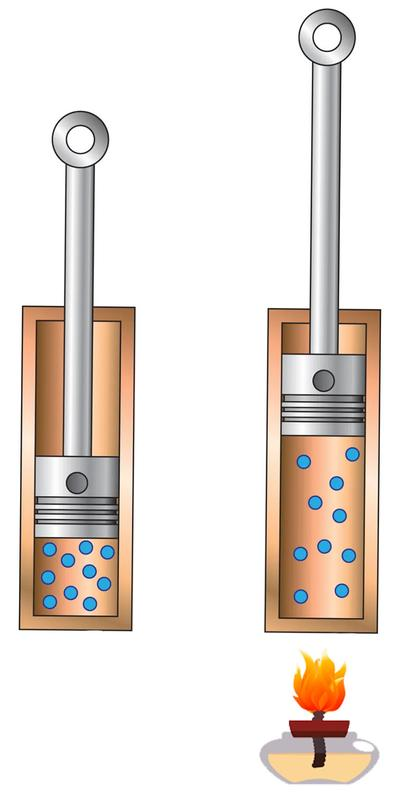
\includegraphics[width=3cm]{Images/xilanh3}}
	
	%	}{\begin{tikzpicture}[rotate=90,scale=.7,thick,>=stealth']
		%	\tkzDefPoints{0/0/o, -2.15/-0.1/a, -1.25/-0.1/b}
		%	\draw (0,0) -- (-3.5,0) -- (-3.5,1) -- (0,1);
		%	\draw (-0.75,1) -- (-0.75,0);
		%	\draw (-1.25,1) -- (-1.25,0);
		%	\fill[pattern=north east lines] (-1.25,0)rectangle(-0.75,1);
		%	\draw[dashed] (-1.75,1) -- (-1.75,0);
		%	\draw[dashed] (-2.15,1) -- (-2.15,0);
		%		(a) -- (b) node [black,midway,yshift=-15pt] 
		%	{};
		%	\end{tikzpicture}}
\loigiai{
	\begin{itemize}
		\item Gọi $\mathrm{S}$ là diện tích tiết diện thẳng của xi-lanh, $h$ là quãng đường pit-tông dịch chuyển, $\mathrm{p}$ là áp suất khí trong xi-lanh. 
		\item Công mà chất khí thực hiện có độ lớn là:
		$$
		\begin{aligned}
			|\mathrm{A}| & =\text { F.h }=\text { p.S.h }=\text { p. } \Delta \mathrm{V} \\
			& =8 . 10^6 .0,5=4 . 10^6 \mathrm{~J} .
		\end{aligned}
		$$	
		\item Vì chất khí thực hiện công và nhận nhiệt nên:
		$$
		\mathrm{Q}>0, \mathrm{~A}<0
		$$
		\item Ta có:
		$$
		\begin{aligned}
			\Delta \mathrm{U} & =\mathrm{A}+\mathrm{Q} \\
			& =-4.10^6+6.10^6=2.10^6\ J
		\end{aligned}
		$$
		\item Vậy độ biến thiên nội năng của khí là:
		$$
		\Delta \mathrm{U}=2.10^6\ J
		$$
	\end{itemize}
	%		\begin{center}
		%			
\includegraphics[width=4cm]{images/2024_04_20_47fa5b18dc83027611bdg-05(4)}
		%		\end{center}
	
}
\haidong{8}\end{ex}
\begin{ex} \nguon{3}
\immini[thm]{Cung cấp nhiệt lượng $1,5\ J$ cho một khối khí trong một xi-lanh đặt nằm ngang. Chất khí nở ra, đẩy pit-tông đi đều một đoạn $5\ cm$. Biết tổng lực cản lên pit-tông có độ lớn không đổi là $20\ N$.}{
\includegraphics[width=4cm]{images/2024_06_05_4d47cfee1d5b1f81200bg-18}}

\begin{chc}
	Công mà khối khí đã thực hiện là
	\choice
	{\True $1\ J$}
	{$0,75\ J$}
	{$-1\ J$}
	{$2\ J$}
	\loigiai{
		\begin{itemize}
			\item[A] Đúng. $A' = F.\ell = 20.0,05 = 1\ J$
			\item[B] Sai. Nhầm trong nhân lực với khoảng cách hoặc làm tròn sai.
			\item[C] Sai. Công thực hiện có thể âm, nhưng câu hỏi yêu cầu **độ lớn** nên kết quả phải là số dương.
			\item[D] Sai. Gấp đôi công thực hiện thực tế.
		\end{itemize}
	}
\end{chc}

\begin{chc}
	Độ biến thiên nội năng của khối khí là
	\choice
	{$1\ J$}
	{$1,5\ J$}
	{\True $0,5\ J$}
	{$2\ J$}
	\loigiai{
		\begin{itemize}
			\item[A] Sai. Đây là độ lớn công, không phải nội năng.
			\item[B] Sai. Đây là toàn bộ nhiệt lượng truyền vào, chưa trừ công thực hiện.
			\item[C] Đúng. $\Delta U = Q + A = 1,5 + (-1) = 0,5\ J$
			\item[D] Sai. Tính sai khi cộng hoặc nhầm dấu của công.
		\end{itemize}
	}
\end{chc}

\end{ex}
\begin{ex} \nguon{4}
Một khối khí được đặt trong một xi-lanh nằm ngang, được đậy kín bằng một pit-tông. Người ta cung cấp cho khối khí một nhiệt lượng $2,5 \ J$. Lúc này khối khí nở ra và đẩy pit-tông dịch chuyển (coi là chuyển động đều) một đoạn $6 \ cm$. Biết rằng tổng lực cản lên pit-tông có độ lớn $F_{c}=10 \ N$. Độ biến thiên nội năng của khối khí bằng bao nhiêu jun (làm tròn kết quả đến chữ số hàng phần mười)?\\
\shortans[oly]{1,9} 
\loigiai{
	\begin{itemize}
		\item Pit-tông chuyển động đều nên lực đẩy pit-tông bằng tổng lực cản: $F=F_{c}=10 \ N$
		\item Công do khối khí thực hiện: $A=F. s=0,6 \ J$
		\item Khối khí nhận nhiệt lượng và thực hiện công, do đó: $Q>0$ và $A<0$
		\item Độ biến thiên nội năng của khối khí: $\Delta U=Q+A=2,5-0,6=1,9 \ J$
		\item Vậy nội năng của khối khí tăng thêm $1,9 \ J$.
	\end{itemize}
}
\end{ex}
\begin{ex}
Một lượng khí nhận nhiệt lượng $250 \ kJ$ do được đun nóng, đồng thời nhận công $500 \ kJ$ do bị nén.
\choiceTF[t]
{Nội năng của khí bị thay đổi chỉ bằng cách truyền nhiệt}
{Theo quy ước: $Q=250 \ kJ$ và $A=-500 \ kJ$}
{\True Độ tăng nội năng của lượng khí là $\Delta U=750 \ kJ$}
{\True Nếu chỉ cung cấp nhiệt lượng $250 \ kJ$ cho lượng khí trên, lượng khí này giãn ra và thực hiện công $100 \ kJ$ lên môi trường xung quanh thì độ biến thiên nội năng của lượng khí là $\Delta U=150 \ kJ$}
\loigiai{
	\begin{itemchoice}
		\itemch SAI. Nội năng của khí tăng do nhận công và nhận nhiệt.
		\itemch SAI. Theo quy ước $Q=250 \ kJ$ và $A=500 \ kJ$.
		\itemch ĐÚNG. $\Delta U=A+Q=750 \ kJ$ 
		\itemch ĐÚNG. $\Delta U=A+Q=250-100=150 \ kJ$ 
	\end{itemchoice}
}
\haidong{12}\end{ex}
\begin{ex}
Người ta cung cấp nhiệt lượng 1,5 J cho chất khí đựng trong một xi-lanh đặt nằm ngang. Chất khí nở ra, đẩy pit-tông đi đều một đoạn $5 \ cm$. Biết lực cản tác dụng lên pit-tông có độ lớn là 20 N. Bỏ qua áp suất không khí bên ngoài xi-lanh.
\choiceTF[t]
{Chất khí nhận một công $A=1 \ J$}
{Theo quy ước, chất khí nhận nhiệt lượng nên $Q=-1,5 \ J$}
{\True Độ biến thiên nội năng của chất khí: $\Delta U=0,5 \ J$}
{\True Chất khí nhận nhiệt, sinh công làm tăng nội năng của hệ}
\loigiai{
	\begin{itemchoice}
		\itemch SAI. Chất khí nở ra nên sinh công chứ không nhận công.
		\itemch SAI. Chất khí nhận nhiệt lượng nên $Q>0\Rightarrow Q=1,5 \ J$.
		\itemch ĐÚNG. $\Delta U=A+Q=-1+1,5=0,5\ J$. Vì $\Delta U>0$ nên nội năng tăng.
		\itemch ĐÚNG
	\end{itemchoice}
}
\haidong{11}\end{ex}
\loai{Loại 1. Cơ năng thành nội năng với vật rơi}
\begin{ex}
	Một quả bóng khối lượng $100\ g$ rơi tự do từ độ cao $10\ m$ xuống mặt sân nằm ngang và nảy lên đến độ cao $7\ m$. Lấy $g=10\ m/s^2$. Độ biến thiên nội năng của quả bóng và sân là
	\choice
	{$30\ J$}
	{$7\ J$}
	{\True $3\ J$}
	{$70\ J$}
	\loigiai{
		\begin{itemize}
			\item Chọn mốc thế năng tại mặt đất.
			\item Phần cơ năng của quả bóng mất đi chuyển thành nội năng của quả bóng: 
			\begin{align*} \Delta U = U_2-U_1=mgz_1-mgz_2\Rightarrow \Delta U=mg(z_1-z_2)=0,1.10.(10-7)=3\ J.
			\end{align*}
		\end{itemize}
	}
	\haidong{4}\end{ex}
\loai{Loại 1. Cơ năng thành nội năng với vật rơi}
%\begin{ex}%[1P6B2-1][Loai3]
%	Nội năng của vật nào tăng lên nhiều nhất khi ta thả rơi từ cùng một độ cao xuống đất 4 vật cùng thể tích. Biết khối lượng riêng của các chất giảm theo thứ tự niken, sắt, kẽm, nhôm. Coi như toàn bộ độ giảm cơ năng chuyển hết thành nội năng của vật.
%	\choice
%	{Vật bằng sắt}
%	{Vật bằng kẽm}
%	{Vật bằng nhôm}
%	{\True Vật bằng niken}
%	\loigiai{ 
	%		\begin{itemize}
		%			\item Các vật ở cùng độ cao sẽ có thế năng càng lớn khi khối lượng càng lớn.
		%			\item Với các vật có cùng thể tích thì những vật có khối lượng riêng càng lớn sẽ có khối lượng càng lớn, do đó vật bằng niken có khối lượng lớn nhất $\Leftrightarrow $ thế năng lớn nhất.
		%			\begin{align*}
			%			\rho=\dfrac{m}{V};\quad W_t=mgh=\rho V gh 
			%			\end{align*}
		%			\item Khi va chạm với mặt đất, thế năng của các vật chuyển thành nhiệt làm thay đổi nội năng của hệ. 
		%			\item Vì vật bằng niken có thế năng lớn nhất nên nội năng sẽ tăng lên nhiều nhất.
		%		\end{itemize}
	%	}
%	%<MyLT>
%	\haidong{2}\end{ex}
\begin{ex}
Một quả bóng rơi từ độ cao $10\ m$ xuống sân và nảy lên đến độ cao $7\ m$. Sở dĩ bóng không nảy lên được tới độ cao ban đầu là vì một phần cơ năng của quả bóng đã chuyển hóa thành nội năng của
\choice
{quả bóng và của sân}
{quả bóng và không khí}
{sân và không khí}
{\True quả bóng, mặt sân và không khí}
\loigiai{
	Khi quả bóng rơi xuống sân và nảy lên, không phải tất cả năng lượng cơ học chuyển động của quả bóng được lưu giữ. Một phần năng lượng được chuyển hóa thành nhiệt năng, hay nội năng. Những yếu tố như sự biến dạng của quả bóng, sự biến dạng cục bộ của mặt sân và lực cản của không khí đều tham gia vào quá trình chuyển hóa này, làm cho năng lượng cơ học bị mất đi và chuyển thành nội năng của cả ba đối tượng: quả bóng, mặt sân, và không khí.
}
\haidong{4}\end{ex}


%\begin{ex}
%	Một vận động viên nhảy cầu có khối lượng $60\ kg$ bắt đầu nhảy từ cầu nhảy.  Tính từ vị trí cao nhất, người này dịch chuyển được $5\ m$ thì dừng lại trong bể bơi. Tính độ biến thiên nội năng của vận động viên này. Bỏ qua tất cả các quá trình truyền nhiệt. Lấy $g=10\ m/s^2$.
%	\choice
%	{\True $3000\ J$}
%	{$2500\ J$}
%	{$2000\ J$}
%	{$15000\ J$}
%	\loigiai{
%		\begin{itemize}
	%			\item Chọn mốc thế năng tại nơi vận động viên dừng lại.
	%			\item Phần cơ năng của vận động viên mất đi chuyển thành nội năng của vận động viên: 
	%			\begin{align*} \Delta U = U_2-U_1=mgz_1-mgz_2\Rightarrow \Delta U=mg(z_1-z_2)=60.10.(5-0)=3000\ J.
		%			\end{align*}
	%		\end{itemize}
%		
%	}
%	\haidong{4}\end{ex}


\begin{ex} \nguon{1}
Một hòn bi thép có trọng lượng $0,5 \ N$ rơi từ độ cao $2 \ m$ xuống một tấm đá rồi nảy lên tới độ cao $1,4 \ m$. Phần cơ năng đã chuyển hóa thành nội năng của bi, tấm đá và không khí là bao nhiêu jun (làm tròn kết quả đến chữ số hàng phần mười)?
\shortans[oly]{0,3}
\loigiai{
\begin{itemize}
	\item Chọn mốc thế năng tại mặt tấm đá.
	\item Cơ năng ban đầu: $W=P . h=0,5 . 2=1 J$.
	\item Cơ năng sau khi bi nảy lên: $W'=P . h'=0,5 . 1,4=0,7 J$.
	\item Phần cơ năng đã chuyển thành nội năng: $\Delta W=W-W'=1-0,7=0,3 J$.\end{itemize}
	}
\end{ex}
\begin{ex} \nguon{4}
Một viên bi có khối lượng $m=100 \ g$ được thả từ độ cao $h_1=10 \ m$ xuống mặt sân thì nảy lên đến được độ cao $h_2=4 \ m$, lấy $g=10 \ m/s^2$. Độ biến thiên nội năng của viên bi, mặt sân và không khí là bao nhiêu jun?
\shortans[oly]{ 6} 
\loigiai{
Độ biến thiên nội năng của hệ viên bi, mặt sân và không khí:
$\Delta U=E_1-E_2=m g\left(h_1-h_2\right)=6\ J$.
}
\end{ex}

\begin{ex} \nguon{4}
Một vận động viên nhảy cầu có khối lượng $m=55 \ kg$ thực hiện động tác nhảy cầu từ độ cao $5 \ m$ xuống một bể bơi. Bỏ qua sự trao đổi nhiệt của nước trong bể bơi với môi trường bên ngoài, lấy $g=10 \ m/s^2$.
\choiceTF[t]
{Nội năng của nước trong bể bơi thay đổi chủ yếu là do quá trình truyền nhiệt từ cơ thể vận động viên sang nước trong bể bơi}
{Độ biến thiên của nước trong bể bằng độ biến thiên nội năng của cơ thể vận động viên}
{Cơ thể vận động viên đã truyền một nhiệt lượng là $2750 \ J$ cho bể nước}
{\True Độ biến thiên nội năng của nước trong bể bơi là $2750 \ J$}
\loigiai{
\begin{enumerate}[label=\alph*)]
	\item Sai. Nội năng thay đổi chủ yếu là do quá trình thực hiện công.
	\item Sai. Độ biến thiên nội năng của nước bằng công do vận động.
	\item Sai. Gần như không có quá trình truyền công do vận động viên thực hiện.
	\item Đúng. Áp dụng công thức $\Delta U$ truyền nhiệt trong trường hợp này.
\end{enumerate}
}
\end{ex}

\begin{ex} \nguon{4}
Một quả bóng khối lượng $150 \ g$ rơi từ độ cao $15 \ m$ xuống sân và nảy lên được $12 \ m$. Lấy $g=10 \ m/s^2$. Độ biến thiên nội năng của quả bóng, mặt sân và không khí xung quanh là
\choice
{\True 4,5 J}
{$12 \ J$}
{15 J}
{$3 \ J$}
\loigiai{
Độ biến thiên nội năng: $\Delta U = mgh_1 - mgh_2 = 0.15 . 10 . (15 - 12) = 4,5 \ J$.
}
\end{ex}

\loai{Loại 2. Cơ năng thành nội năng khi đạn bắn vào tường}

\loai{Loại 3. Cơ năng thành nội năng trên mpn}
\begin{ex} \nguon{3}
\immini[thm]{Một vật khối lượng 1 kg trượt không vận tốc ban đầu từ đỉnh một mặt phẳng nghiêng dài 0,80 $m$ góc nghiêng $30^\circ$ so với phương ngang. Trượt tới chân mặt phẳng nghiêng, vận tốc của vật đạt $1,2\ m/s$. Lấy $g=9,8\ m/s^2$. Bỏ qua sự trao đổi nhiệt với mặt phẳng nghiêng. Độ biến thiên nội năng của vật trong quá trình nói trên bằng
\choice
{$7,02\ J$}
{\True $3,2\ J$}
{$3,92\ J$}
{$6,4\ J$}}{\begin{tikzpicture}[scale=1,thick,>=stealth']
	\tkzDefPoints{0/0/o,4/0/a, 4/1.5/b, -0.05/0.19/o', 3.85/1.67/b'}
	\tkzDrawSegments[](a,b o,a o,b)
	\node [draw, thick, shape=rectangle,fill=orange, minimum width=0.5cm, minimum height=0.4cm, anchor=center,rotate=20] at (o') {};
	\node [draw, thick, shape=rectangle,fill=orange, minimum width=0.5cm, minimum height=0.4cm, anchor=center,rotate=20] at (b') {};
	\tkzMarkAngles[size=0.9cm](a,o,b)
	\tkzLabelAngles[pos=1.3](a,o,b){$30^\circ$}
	\node[rotate=20] at (2.5,0.7) {$0,8\ m$};
	\node at (-0.15,0.85) {$v=1,2\ m/s$};
	\node at (3.8,2.3) {$v_0=0\ m/s$};
	\end{tikzpicture}}
	\loigiai{
Tại đỉnh mặt phẳng nghiêng, vật ở độ cao: $h=\ell \sin \alpha=0,8 \sin 30^\circ=0,4 m$
\begin{itemize}
	\item Công của ngoại lực tác dụng lên vật: $A=mgh-\dfrac{1}{2} mv^2=1 . (9,8 . 0,4 - \dfrac{1}{2} . 1,2^2)=3,2 J$
	\item Do vật không trao đổi nhiệt với môi trường bên ngoài nên độ biến thiên nội năng của vật: $\Delta U=A=3,2 J$ (nội năng của vật tăng)
\end{itemize}
}
\end{ex}

\loai{Loại 4. Va chạm}
\section{Nhiệt độ}
\subsection{Lí thuyết}
\begin{ex}
	Đơn vị đo nhiệt độ trong thang nhiệt độ Celsius là
	\choice
	{$\ K$}
	{$^\circ F$}
	{$^\circ N$}
	{\True $^\circ C$}
	\loigiai{
		Đơn vị đo nhiệt độ trong thang nhiệt Celsius là độ Celsius, ký hiệu là $^\circ C$.
	}
	\haidong{2}
\end{ex}

\begin{ex}
	Theo thang nhiệt độ Celsius, từ nhiệt độ đông đặc đến nhiệt độ sôi của nước được chia thành
	\choice
	{\True 100 phần bằng nhau, mỗi phần ứng với $1^\circ C$}
	{100 phần bằng nhau, mỗi phần ứng với $1\ K$}
	{100 phần bằng nhau, mỗi phần ứng với $1\ F$}
	{10 phần bằng nhau, mỗi phần ứng với $1^\circ C$}
	\loigiai{
		Thang nhiệt Celsius chia khoảng từ điểm đóng băng ($0^\circ C$) đến điểm sôi ($100^\circ C$) của nước thành 100 phần bằng nhau, mỗi phần ứng với $1^\circ C$.
	}
	\haidong{2}
\end{ex}

\begin{ex}
	Đơn vị đo nhiệt độ thường dùng ở Việt Nam là
	\choice
	{Kelvin (Kí hiệu K)}
	{\True Độ Celsius (Kí hiệu $^\circ C$)}
	{Độ Fahrenheit (Kí hiệu F)}
	{Cả 3 đáp án trên đều sai}
	\loigiai{
		Tại Việt Nam, đơn vị đo nhiệt độ thông dụng là độ Celsius, ký hiệu là $^\circ C$.
	}
	\haidong{2}
\end{ex}
\begin{ex}
	Thang nhiệt độ Celsius có nhiệt độ âm là nhiệt độ
	\choice
	{\True thấp hơn $0^\circ C$}
	{cao hơn $0^\circ C$}
	{từ $35^\circ C$ đến $42^\circ C$}
	{từ $0^\circ C$ đến $100^\circ C$}
	\loigiai{
		Nhiệt độ âm trên thang Celsius là những giá trị nhiệt độ thấp hơn điểm đóng băng của nước, tức là thấp hơn $0^\circ C$.
	}
	\haidong{2}\end{ex}



\begin{ex}
	Điểm đóng băng và sôi của nước theo thang Kelvin xấp xỉ là
	\choice
	{$0\ K$ và $100\ K$}
	{\True $273\ K$ và $373\ K$}
	{$73\ K$ và $37\ K$}
	{$32\ K$ và $212\ K$}
	\loigiai{
		Điểm đóng băng của nước trong thang Kelvin là $273 \ K$ và điểm sôi của nước là $373 \ K$.
	}
	\haidong{3}\end{ex}


\begin{ex}
	Nhiệt độ không tuyệt đối là nhiệt độ tại đó 
	\choice
	{\True các phân tử không chuyển động nhiệt}
	{nước đông đặc thành đá}
	{tất cả các chất khí hóa rắn}
	{tất cả các chất khí hóa lỏng}
	\loigiai{
		Nhiệt độ không tuyệt đối là nhiệt độ tại đó các phân tử không còn chuyển động nhiệt, tức các phân tử có động năng bằng 0.
	}
	\haidong{2}\end{ex}
\begin{ex}
	Điểm đóng băng và sôi của nước theo thang Fahrenheit là
	\choice
	{$0^\circ F$ và $100^\circ F$}
	{$100^\circ F$ và $200^\circ F$}
	{\True $32^\circ F$ và $212^\circ F$}
	{$22^\circ F$ và $202^\circ F$}
	\loigiai{
		Thang Fahrenheit xác định điểm đóng băng của nước là $32^\circ F$ và điểm sôi của nước là $212^\circ F$.
	}
	\haidong{2}\end{ex}

\begin{ex}
	Nhiệt kế là thiết bị dùng để đo?
	\choice
	{Chiều dài}
	{Thể tích}
	{\True Nhiệt độ}
	{Diện tích}
	\loigiai{
		Nhiệt kế là thiết bị dùng để đo nhiệt độ.
	}
	\haidong{2}\end{ex}



\begin{ex}
	Nhiệt kế nào sau đây hoạt động dựa trên hiện tượng dãn nở vì nhiệt của chất lỏng?
	\choice
	{\True Nhiệt kế thủy ngân}
	{Nhiệt kế kim loại}
	{Nhiệt kế hồng ngoại}
	{Nhiệt kế điện tử}
	\loigiai{
		Nhiệt kế thủy ngân hoạt động dựa trên hiện tượng dãn nở vì nhiệt của chất lỏng (thủy ngân).
	}
	\haidong{2}\end{ex}

\begin{ex}
	Trong các nhiệt kế sau đây, em hãy chọn nhiệt kế phù hợp để đo nhiệt độ của nước sôi?
	\choice
	{Nhiệt kế y tế có thang chia độ từ $35^\circ C$ đến $42^\circ C$}
	{Nhiệt kế rượu có thang chia độ từ $-30^\circ C$ đến $60^\circ C$}
	{\True Nhiệt kế thuỷ ngân có thang chia độ từ $-10^\circ C$ đến $110^\circ C$}
	{Nhiệt kế hồng ngoại có thang chia độ từ $30^\circ C$ đến $45^\circ C$}
	\loigiai{
		Để đo nhiệt độ của nước sôi, cần dùng nhiệt kế thủy ngân có thang chia độ từ $-10^\circ C$ đến $110^\circ C$ vì nhiệt độ sôi của nước nằm trong khoảng đo này.
	}
	\haidong{2}\end{ex}



\begin{ex}
	Phát biểu nào sau đây là \textbf{sai}? Nhiệt kế thuỷ ngân dùng để đo
	\choice
	{\True nhiệt độ của lò luyện kim đang hoạt động}
	{nhiệt độ của nước đá đang tan}
	{nhiệt độ khí quyển}
	{nhiệt độ cơ thể người}
	\loigiai{
		Nhiệt kế thủy ngân không thể dùng để đo nhiệt độ của lò luyện kim đang hoạt động vì giới hạn nhiệt độ đo của nó thấp hơn nhiều so với nhiệt độ trong lò luyện kim.
	}
	\haidong{2}\end{ex}
\begin{ex}
	So sánh nhiệt độ của một vật nóng với nhiệt độ của một vật lạnh thì
	\choice
	{nhiệt độ  của vật lạnh cao hơn nhiệt độ của vật nóng}
	{\True nhiệt độ của vật lạnh thấp hơn nhiệt độ của vật nóng}
	{nhiệt độ  của vật lạnh bằng nhiệt độ của vật nóng}
	{nhiệt độ  của vật nóng thấp hơn nhiệt độ của vật lạnh}
	\loigiai{
		Nhiệt độ của vật lạnh thấp hơn nhiệt độ của vật nóng
	}
	\haidong{3}\end{ex}


\begin{ex}
	Cho các bước như sau:
	\begin{itemize}
		\item[(1)] Thực hiện phép đo nhiệt độ.
		\item[(2)] Ước lượng nhiệt độ của vật.
		\item[(3)] Hiệu chỉnh nhiệt kế.
		\item[(4)] Lựa chọn nhiệt kế phù hợp.
		\item[(5)] Đọc và ghi kết quả đo.
	\end{itemize}
	Các bước đúng khi thực hiện đo nhiệt độ của một vật là
	\choice
	{\True (2), (4), (3), (1), (5)}
	{(1), (4), (2), (3), (5)}
	{(1), (2), (3), (4), (5)}
	{(3), (2), (4), (1), (5)}
	\loigiai{
		Các bước tiến hành đo nhiệt độ đúng là: 
		\begin{itemize}
			\item (2) Ước lượng nhiệt độ của vật để có thể chọn loại nhiệt kế phù hợp.
			\item (4) Lựa chọn nhiệt kế phù hợp với khoảng nhiệt độ ước lượng.
			\item (3) Hiệu chỉnh nhiệt kế để đảm bảo chính xác.
			\item (1) Thực hiện phép đo nhiệt độ.
			\item (5) Đọc và ghi kết quả đo.
		\end{itemize}
	}
	\haidong{2}\end{ex}







\begin{ex}%(BT) 
	Nhỏ một giọt nước đang sôi vào một cốc nước lạnh thì nhiệt năng của giọt nước và nước trong cốc thay đổi như thế nào?
	\choice
	{Nhiệt năng của giọt nước tăng, của nước trong cốc giảm}
	{\True Nhiệt năng của giọt nước giảm, của nước trong cốc tăng}
	{Nhiệt năng của giọt nước và nước trong cốc đều giảm}
	{Nhiệt năng của giọt nước và nước trong cốc đều tăng}
	\loigiai{
		Khi giọt nước đang sôi (nhiệt độ cao) được cho vào cốc nước lạnh (nhiệt độ thấp hơn), nhiệt sẽ truyền từ giọt nước sôi sang nước trong cốc. Kết quả là nhiệt năng của giọt nước giảm và nhiệt năng của nước trong cốc tăng.
	}
	\haidong{2}\end{ex}





\begin{ex}
	Cho hai vật có nhiệt độ khác nhau tiếp xúc với nhau thì nhiệt được truyền từ vật 
	\choice
	{có khối lượng lớn hơn sang vật có khối lượng nhỏ hơn}
	{\True có nhiệt độ cao hơn sang vật có nhiệt độ thấp hơn}
	{có nhiệt năng lớn hơn sang vật có nhiệt năng nhỏ hơn}
	{ở trên cao sang vật ở dưới thấp}
	\loigiai{
		Nhiệt chỉ có thể truyền từ vật có nhiệt độ cao hơn đến vật có nhiệt độ thấp hơn cho đến khi đạt đến trạng thái cân bằng nhiệt độ. Do đó, câu trả lời đúng là nhiệt được truyền từ vật có nhiệt độ cao hơn sang vật có nhiệt độ thấp hơn.
	}
	\haidong{3}\end{ex}


\begin{ex}
	Cho các nhiệt độ sau: $0^\circ C;\ 5^\circ C;\ 36,5^\circ C;\ 327^\circ C$. Đó là nhiệt độ có thể thích hợp cho lần lượt từng trường hợp nào sau đây?
	\choice
	{Chì nóng chảy, nhiệt độ cơ thể người, ly nước trà đá, nước đá}
	{Ly nước trà đá, nước đá, chì nóng chảy, nhiệt độ cơ thể người}
	{Nước đá, ly nước trà đá, chì nóng chảy, nhiệt độ cơ thể người}
	{\True Nước đá, ly nước trà đá, nhiệt độ cơ thể người, chì nóng chảy}
	\loigiai{
		- $0^\circ C$: Nhiệt độ đông đặc của nước, tức là nhiệt độ của nước đá. \\
		- $5^\circ C$: Nhiệt độ điển hình cho một ly nước trà đá. \\
		- $36,5^\circ C$: Nhiệt độ cơ thể người bình thường. \\
		- $327^\circ C$: Nhiệt độ nóng chảy của chì. 
		
		Do đó, trật tự đúng là: nước đá ($0^\circ C$), ly nước trà đá ($5^\circ C$), nhiệt độ cơ thể người ($36,5^\circ C$), chì nóng chảy ($327^\circ C$).
	}
	\haidong{3}\end{ex}


\begin{ex} \nguon{2}
	Việc ước lượng nhiệt độ trước khi đo có tác dụng gì?
	\choice
	{Giúp đảm bảo an toàn khi đo nhiệt độ}
	{Giúp chọn được nhiệt kế đo phù hợp trong các trường hợp khác nhau}
	{Giúp cho mình không cần đo nhiệt độ của vật nữa}
	{\True Cả hai đáp án $A$ và $B$ đều đúng}
	
	\loigiai{
		\begin{itemize}
			\item Ước lượng nhiệt độ trước khi đo giúp không bị bỏng khi chạm tay vào vật.
			\item Ước lượng nhiệt độ trước khi đo giúp chọn được nhiệt kế đo phù hợp trong các trường hợp khác nhau.
			\item Do đó, cả hai đáp án đều đúng.
		\end{itemize}
	}
\end{ex}


\begin{ex} \nguon{2}
	Khi dùng nhiệt kế để đo nhiệt độ của chính cơ thể mình, người ta phải thực hiện các thao tác sau (chưa được sắp xếp theo đúng thứ tự):
	\begin{itemize}
		\item [a)] Đặt nhiệt kế vào nách trái, rồi kẹp cánh tay lại để giữ nhiệt kế.
		\item [b)] Lấy nhiệt kế ra khỏi nách để đọc nhiệt độ.
		\item [c)] Dùng bông lau sạch thân và bầu nhiệt kế.
		\item [d)] Kiểm tra xem thuỷ ngân đã tụt hết xuống bầu nhiệt kế chưa. Nếu chưa, thì vẩy nhiệt kế cho thuỷ ngân tụt xuống.
	\end{itemize}
	Hãy sắp xếp các thao tác trên theo thứ tự hợp lí nhất.
	\choice
	{$a,\ b,\ c,\ d$}
	{\True $d,\ c,\ a,\ b$}
	{$d,\ c,\ b,\ d$}
	{$b,\ a,\ c,\ d$}
	\loigiai{
		\begin{itemize}
			\item [d)] Kiểm tra xem thuỷ ngân đã tụt hết xuống bầu nhiệt kế chưa. Nếu chưa, thì vẩy nhiệt kế cho thuỷ ngân tụt xuống.
			
			\item [c)] Dùng bông lau sạch thân và bầu nhiệt kế.
			
			\item [a)] Đặt nhiệt kế vào nách trái, rồi kẹp cánh tay lại để giữ nhiệt kế.
			
			\item [b)] Lấy nhiệt kế ra khỏi nách để đọc nhiệt độ.
		\end{itemize}	
	}
\end{ex}








\begin{ex} \nguon{2}
	Phát biểu nào sau đây là \textbf{sai}?
	\choice
	{Nhiệt kế kim loại dùng dể đo nhiệt độ của bàn là}
	{Nhiệt kế rượu dùng để đo nhiệt độ không khí trong phòng}
	{\True Nhiệt kế thuỷ ngân dùng để đo của một lò luyện kim}
	{Nhiệt kế y tế dùng để đo nhiệt độ của người}
	\loigiai{
		\begin{itemize}
			\item Nhiệt độ ở 1 lò luyện kim là rất lớn, cao hơn giới hạn đo của nhiệt kế thủy ngân. 
			\item Vì vậy, không dùng nhiệt kế thủy ngân để đo nhiệt độ lò luyện kim được.
		\end{itemize}
	}
\end{ex}




















\begin{ex} \nguon{2}
	Cho hai nhiệt kế rượu và thủy ngân. Dùng nhiệt kế nào có thể đo được nhiệt độ của nước đang sôi? Cho biết nhiệt độ sôi của rượu và thủy ngân lần lượt là $80^\circ C$ và $357^\circ C$.
	\choice
	{Cả nhiệt kế thủy ngân và nhiệt kế rượu}
	{Không thể dùng nhiệt kế thủy ngân và nhiệt kế rượu}
	{Nhiệt kế rượu}
	{\True Nhiệt kế thủy ngân}
	\loigiai{
		\begin{itemize}
			\item Nhiệt độ sôi của nước: $100^\circ C$.
			\item Nhiệt kế rượu có thể đo nhiệt độ lên đến $80^\circ C$, vì nhiệt độ sôi của rượu là $80^\circ C$. Do đó, nhiệt kế rượu không thể đo được nhiệt độ của nước đang sôi, vì nước sôi ở $100^\circ C$, cao hơn nhiệt độ sôi của rượu.
			\item Nhiệt kế thủy ngân có thể đo nhiệt độ lên đến $357^\circ C$, vì nhiệt độ sôi của thủy ngân là $357^\circ C$. Do đó, nhiệt kế thủy ngân có thể đo được nhiệt độ của nước đang sôi.
		\end{itemize}
	}
\end{ex}

\begin{ex} \nguon{2}
	Thao tác nào sau đây \textbf{chưa} chính xác khi dùng nhiệt kế thủy ngân?
	\choice
	{Vẩy mạnh nhiệt kế trước khi đo}
	{Dùng tay nắm chặt bầu nhiệt kế một lúc rồi mới đo}
	{Nhiệt kế kẹp nách được 30 s đã mang nhiệt kế ra đọc}
	{\True Cả hai đáp án $B$ và $C$ đều chưa chính xác}
	
	\loigiai{
		\begin{itemize}
			\item Dùng tay nắm chặt bầu nhiệt kế một lúc rồi mới đo là chưa chính xác vì sẽ làm nhiệt kế hiển thị sai kết quả.
			\item Nhiệt kế kẹp nách cần được giữ ít nhất 3 phút, kẹp chỉ 30 giây là chưa chính xác.
			\item Do đó, cả hai thao tác đều chưa chính xác.
		\end{itemize}
	}
\end{ex}

\begin{ex} \nguon{2}
	Sắp xếp đúng thứ tự các bước đo nhiệt độ bằng nhiệt kế điện tử.
	\begin{itemize}
		\item [(1)] Tắt nút khởi động.
		\item [(2)] Lau sạch đầu kim loại của nhiệt kế.
		\item [(3)] Bấm nút khởi động.
		\item [(4)] Chờ khi có tín hiệu bíp, rút nhiệt kế ra đọc nhiệt độ.
		\item [(5)] Đặt đầu kim loại của nhiệt kế xuống lưỡi.
	\end{itemize}
	\choice
	{(1), (2), (3), (4), (5)}
	{\True (2), (3), (5), (4), (1)}
	{(2), (1), (3), (4), (5)}
	{(1), (2), (5),(4), (3)}
	
	\loigiai{
		Các bước đo nhiệt độ bằng nhiệt kế điện tử cần sắp xếp đúng thứ tự để bảo đảm đo chính xác và vệ sinh:
		\begin{itemize}
			\item Lau sạch đầu kim loại của nhiệt kế.
			\item Bấm nút khởi động.
			\item Đặt đầu kim loại của nhiệt kế xuống lưỡi.
			\item Chờ khi có tín hiệu bíp, rút nhiệt kế ra đọc nhiệt độ.
			\item Tắt nút khởi động.
		\end{itemize}
	}
\end{ex}


\begin{ex} \nguon{2}
	Phát biểu nào sau đây \textbf{không} đúng?
	\choice
	{Nhiệt kế y tế có thể dùng để đo nhiệt độ cơ thể người}
	{\True Nhiệt kế thủy ngân có thể dùng để đo nhiệt độ trong lò luyện kim}
	{Nhiệt kế kim loại có thể đo nhiệt độ của bàn là đang nóng}
	{Nhiệt kế rượu có thể dùng để đo nhiệt độ của khí quyển}
	\loigiai{
		\begin{itemize}
			\item Nhiệt kế thủy ngân có thể đo được nhiệt độ rất cao (lên đến $357^\circ C$). Tuy nhiên, trong lò luyện kim, nhiệt độ có thể vượt quá giới hạn này, thường từ $1.000^\circ C$ đến $2.000^\circ C$. 
			\item Vì vậy, phát biểu này chỉ đúng trong một số trường hợp nhất định và có thể gây hiểu lầm nếu không rõ ràng về phạm vi nhiệt độ trong lò luyện kim.
		\end{itemize}
	}
\end{ex}

\begin{ex} \nguon{2}
	Khi nhúng một nhiệt kế rượu vào nước nóng, mực rượu trong ống nhiệt kế tăng lên vì
	\choice
	{ống nhiệt kế dài ra}
	{ống nhiệt kế ngắn lại}
	{\True cả ống nhiệt kế và rượu trong ống đều nở ra nhưng rượu nở nhiều hơn}
	{cả ống nhiệt kế và rượu trong ống đều nở ra nhưng ống nhiệt kế nở nhiều hơn}
	\loigiai{
		Cả hai đều giãn nở nhưng rượu giãn nở nhiều hơn so với ống thủy tinh, làm cho mực rượu dâng lên.
	}
\end{ex}


\begin{ex} \nguon{2}
	Quan sát các nhiệt kế thủy ngân và nhiệt kế rượu thấy ở phần trên của nhiệt kế thường phình ra, chỗ phình ra đó có tác dụng
	\choice
	{chứa lượng thủy ngân hoặc rượu khi dâng lên}
	{\True chứa lượng khí còn dư khi thủy ngân hoặc rượu dâng lên}
	{phình ra cho cân đối nhiệt kế}
	{nhìn nhiệt kế đẹp hơn}
	
	\loigiai{
		Chỗ phình ra ở phần trên của nhiệt kế có tác dụng chứa lượng khí còn dư khi thủy ngân hoặc rượu dâng lên. Điều này tránh làm vỡ nhiệt kế khi chất lỏng bị dồn lên quá cao.
	}
\end{ex}

\begin{ex} \nguon{2}
	Theo tính toán, nhiệt độ của chất lỏng phải là $130 \ K$. Tuy nhiên, nhiệt kế trong bình hiển thị nhiệt độ $-143^\circ C$. Điều này có nghĩa là
	\choice
	{nhiệt kế hiển thị nhiệt độ thấp hơn}
	{nhiệt kế hiển thị nhiệt độ cao hơn}
	{\True nhiệt kế hiển thị đúng nhiệt độ đã tính toán}
	{nhiệt kế không được thiết kế cho nhiệt độ thấp và cần được thay thế}
	
	\loigiai{
		Nhiệt độ $-143^\circ C$ khi đổi sang Kelvin là $130 \ K$ (bằng $130 =-143+273$), điều này có nghĩa là nhiệt kế hiển thị đúng nhiệt độ đã tính toán.
	}
\end{ex}



\begin{ex} \nguon{2}
	Có nhiều loại dụng cụ đo nhiệt độ khác nhau, mỗi loại có ưu điểm và hạn chế riêng. Chọn phát biểu đúng về các loại nhiệt kế sau đây?
	\choice
	{\True Nhiệt kế thủy ngân có ưu điểm là giá rẻ, độ chính xác cao nhưng có nhược điểm là dễ vỡ và độc hại khi rò rỉ thủy ngân}
	{Nhiệt kế hồng ngoại chỉ có thể đo nhiệt độ cơ thể con người, không thể đo nhiệt độ của vật thể hay môi trường xung quanh}
	{Nhiệt kế thủy ngân có thể đo nhiệt độ nhanh hơn nhiệt kế hồng ngoại và an toàn hơn khi sử dụng cho trẻ nhỏ}
	{Nhiệt kế hồng ngoại có độ chính xác cao hơn nhiệt kế thủy ngân và không bị ảnh hưởng bởi các yếu tố môi trường}
	\loigiai{
		\begin{itemize}
			\item Nhiệt kế thủy ngân: Ưu điểm đó là phổ biến, giá rẻ và cho độ chính xác cao
			\item Nhiệt kế hồng ngoại: Ưu điểm đó là thời gian đo nhanh, cách sử dụng đơn giản, độ an toàn cao, vị trí đo đa dạng (thường được dùng trong các bệnh viện), ngoài đo thân nhiệt có thể được sử dụng đo nhiệt độ của các vật thể khác, đo nhiệt độ phòng $\ldots$
		\end{itemize}
	}
\end{ex}



\begin{ex} \nguon{2}
	Nhiệt kế nào sau đây có thể dùng để đo nhiệt độ của nước đang sôi?
	\choice
	{\True Nhiệt kế thủy ngân}
	{Nhiệt kế rượu}
	{Nhiệt kế y tế}
	{Cả ba nhiệt kế trên}
	
	\loigiai{
		Nhiệt kế thủy ngân có thể đo nhiệt độ cao tới khoảng 357°C, phù hợp để đo nhiệt độ của nước đang sôi (100°C). Trong khi đó, nhiệt kế rượu không thể đo nhiệt độ cao như vậy.
	}
\end{ex}
\begin{ex} \nguon{2}
	Phát biểu nào sau đây là \textbf{không} đúng với thang nhiệt độ Celsius?
	\choice
	{Kí hiệu của nhiệt độ là t}
	{Chọn mốc nhiệt độ nước đá đang tan ở áp suất $1 \ atm$ là $0^\circ C$}
	{\True $1^\circ C$ tương ứng với $273 \ K$}
	{Đơn vị đo nhiệt độ là ${}^\circ C$}
	
	\loigiai{
		Kết luận $1^\circ C$ tương ứng với $273 \ K$ là không đúng. Thực tế, $0^\circ C$ tương ứng với $273 K$ và $1^\circ C$ tương ứng với $274 K$.
	}
\end{ex}



\begin{ex} \nguon{2}
	Khi nhiệt độ tuyệt đối tăng thêm $6 \ K$ thì
	\choice
	{nhiệt độ Celsius tăng thêm hơn $6^\circ C$}
	{nhiệt độ Celsius tăng thêm $279^\circ C$}
	{\True nhiệt độ Celsius tăng thêm $6^\circ C$}
	{nhiệt độ Celsius tăng thêm $267^\circ C$}
	
	\loigiai{
		Khi nhiệt độ tuyệt đối tăng thêm $6 K$, điều này cũng có nghĩa là nhiệt độ Celsius tăng thêm $6^\circ C$ vì sự thay đổi một độ Kelvin tương ứng với sự thay đổi một độ Celsius.
	}
\end{ex}






\begin{ex} \nguon{2}
	Mỗi độ chia (1 K) trong thang Kelvin bằng $\ldots$ [1] của khoảng cách giữa nhiệt độ không tuyệt đối và nhiệt độ mà nước tinh khiết tồn tại đồng thời ở thể rắn, lỏng và hơi (ở áp suất tiêu chuẩn). [1] cần điền là
	\choice
	{\True $\dfrac{1}{273,16}$}
	{$273,16$}
	{$-\dfrac{1}{273,16}$}
	{$-273,16$}
	
	\loigiai{
		Mỗi độ chia (1 K) trong thang Kelvin bằng $\dfrac{1}{273,16}$ của khoảng cách giữa nhiệt độ không tuyệt đối (0 K) và nhiệt độ ba thể của nước tinh khiết (273,16 K).
	}
\end{ex}

\begin{ex} \nguon{2}
	Mỗi độ chia $\left(1^\circ C\right)$ trong thang Celsius bằng $\ldots$ [1] của khoảng cách giữa nhiệt độ tan chảy của nước tinh khiết đóng băng và nhiệt độ sôi của nước tinh khiết (ở áp suất tiêu chuẩn). [1] cần điền là
	\choice
	{\True $\dfrac{1}{100}$}
	{$100$}
	{$273$}
	{$-273$}
	
	\loigiai{
		Mỗi độ chia $\left(1^\circ C\right)$ trong thang Celsius tương ứng với $\dfrac{1}{100}$ của khoảng cách giữa nhiệt độ tan chảy của nước đá (0°C) và nhiệt độ sôi của nước (100°C).
	}
\end{ex}

\begin{ex} \nguon{2}
	Một vật được làm lạnh từ $100^\circ C$ xuống $0^\circ C$. Nhiệt độ của vật giảm đi theo thang Kelvin là
	\choice
	{\True 100 $K$}
	{$-100$ $K$}
	{Không liên quan}
	{Tùy vào tính chất của vật}
	
	\loigiai{
		Sự thay đổi nhiệt độ trong thang Celsius và thang Kelvin là tương đương. Do đó, khi nhiệt độ của vật giảm từ $100^\circ C$ xuống $0^\circ C$, nhiệt độ theo thang Kelvin cũng giảm đi 100 K.
	}
\end{ex}


\begin{ex} \nguon{3}
	Dụng cụ nào sau đây dùng để đo nhiệt độ?
	\choice
	{Cân đồng hồ}
	{\True Nhiệt kế}
	{Vôn kế}
	{Tốc kế}
	\loigiai{
		\begin{itemize}
			\item Nhiệt kế là dụng cụ dùng để đo nhiệt độ của một vật hay môi trường.
			\item Cân đồng hồ dùng để đo khối lượng.
			\item Vôn kế dùng để đo hiệu điện thế.
			\item Tốc kế dùng để đo tốc độ.
		\end{itemize}
	}
\end{ex}



\begin{ex} \nguon{3}
	Nhiệt kế là thiết bị dùng để đo?
	\choice
	{Chiều dài}
	{Thể tích vật rắn}
	{\True Nhiệt độ}
	{Diện tích}
	\loigiai{
		\begin{itemize}
			\item Nhiệt kế là thiết bị dùng để đo nhiệt độ.
			\item Chiều dài đo bằng thước.
			\item Thể tích vật rắn có thể đo bằng bình chia độ hoặc phương pháp đo thể tích.
			\item Diện tích được đo bằng các dụng cụ như thước hoặc phần mềm tính toán.
		\end{itemize}
	}
\end{ex}


\begin{ex} \nguon{3}
	Phát biểu nào sau đây đúng khi so sánh nhiệt độ của một vật đang nóng với nhiệt độ của một vật đang lạnh?
	\choice
	{Vật lạnh có nhiệt độ cao hơn nhiệt độ của vật nóng}
	{\True Vật lạnh có nhiệt độ thấp hơn nhiệt độ của vật nóng}
	{Vật lạnh có nhiệt độ bằng nhiệt độ của vật nóng}
	{Vật nóng có nhiệt độ thấp hơn nhiệt độ của vật lạnh}
	\loigiai{
		\begin{itemize}
			\item Nhiệt độ của vật lạnh thấp hơn nhiệt độ của vật nóng.
			\item Nhiệt độ là thước đo mức độ "nóng" hay "lạnh" của một vật.
		\end{itemize}
	}
\end{ex}




\begin{ex} \nguon{3}
	Câu nào sau đây nói về nguyên nhân của sự thay đổi nhiệt độ của một vật là đúng? Nhiệt độ của vật giảm là do các nguyên tử, phân tử cấu tạo nên vật
	\choice
	{ngừng chuyển động}
	{nhận thêm động năng}
	{\True chuyển động chậm đi}
	{va chạm vào nhau}
	\loigiai{
		\begin{itemize}
			\item Khi nhiệt độ của vật giảm, các nguyên tử, phân tử cấu tạo nên vật chuyển động chậm đi.
			\item Nhiệt độ của một vật tỷ lệ thuận với động năng trung bình của các phân tử của nó.
			\item Do đó, khi nhiệt độ giảm, động năng trung bình của các phân tử giảm do chúng chuyển động chậm hơn.
		\end{itemize}
	}
\end{ex}



\begin{ex} \nguon{4}
	Nhiệt kế rượu hoạt động dựa trên tính chất nào sau đây của rượu?
	\choice
	{Tính khó chịu nén của rượu}
	{Tính chịu nhiệt của rượu}
	{\True Tính giãn nở đều vì nhiệt của rượu}
	{Tính dễ bay hơi của rượu}
	\loigiai{
		Nhiệt kế rượu hoạt động dựa trên tính giãn nở đều vì nhiệt của rượu.
	}
\end{ex}

\begin{ex} \nguon{2}
	Tại sao bảng chia độ của nhiệt kế y tế lại \textbf{không} có nhiệt độ dưới $34^\circ C$ và trên $42^\circ C$?
	\choice
	{Vì nhiệt kế y tế chỉ được sản xuất với khoảng đo cố định như vậy theo tiêu chuẩn quốc tế}
	{\True Vì cơ thể người có nhiệt độ dao động chủ yếu trong khoảng $35^\circ C$ đến $42^\circ C$, nên không cần đo ngoài khoảng này}
	{Vì dưới $34^\circ C$ và trên $42^\circ C$, thủy ngân trong nhiệt kế không thể giãn nở hoặc co lại chính xác}
	{Vì nhiệt kế y tế không thể đo được nhiệt độ dưới $34^\circ C$ hoặc trên $42^\circ C$ do giới hạn chất lỏng bên trong}
	\loigiai{
		Vì nhiệt kế y tế dùng để đo nhiệt độ cơ thể người, mà cơ thể người có nhiệt độ chỉ trong khoảng từ $35^\circ C$ đến $42^\circ C$.
	}
\end{ex}



\begin{ex} \nguon{4}
	Gọi $t_1,\ t_2$ lần lượt là nhiệt độ điểm đóng băng và nhiệt độ sôi của nước tinh khiết ở điều kiện áp suất tiêu chuẩn. Trong thang nhiệt Celsius, mỗi độ chia $\left(1^\circ C\right)$ có độ lớn bằng
	\choice
	{$100\left(t_2-t_1\right)$}
	{$100\left(t_1-t_2\right)$}
	{\True $\dfrac{1}{100}\left(t_2-t_1\right)$}
	{$\dfrac{1}{100}\left(t_1-t_2\right)$}
	\loigiai{
		\begin{itemize}
			\item Nhiệt độ điểm đóng băng của nước là $0^\circ C$, nhiệt độ sôi là $100^\circ C$.
			\item Trong thang nhiệt Celsius, mỗi độ chia $\left(1^\circ C\right)$ có độ lớn bằng $\dfrac{1}{100}\left(t_2-t_1\right)$.
		\end{itemize}
	}
\end{ex}

\begin{ex} \nguon{4}
	Hai học sinh đang trao đổi về nhiệt độ ở Bắc cực:
	\begin{itemize}
		\item Học sinh 1: "Một số vùng ở Bắc cực nhiệt độ có thể xuống đến âm 45 độ."
		\item Học sinh 2: "Bạn đang nói đến nhiệt độ trong thang nhiệt độ Kelvin hay Celsius?" 
	\end{itemize}
	Hãy cho biết những điều chưa đúng trong hai câu nói trên.
	\loigiai{
		\begin{itemize}
			\item Học sinh 1 trong câu nói của mình chưa nói rõ nhiệt độ nói đến là được ghi nhận theo thang đo nào.
			\item Học sinh 2 hỏi về thang đo nhiệt độ là đúng. Nhưng câu hỏi không mang nhiều ý nghĩa vì trong thang nhiệt Kelvin không có các giá trị nhiệt độ âm.
		\end{itemize}
	}
\end{ex}








\begin{ex} \nguon{4}
	Nguyên tắc hoạt động của các loại nhiệt kế phổ biến như nhiệt kế thủy ngân, nhiệt kế rượu và nhiệt kế điện trở dựa trên yếu tố nào sau đây?
	\choice
	{Cả ba loại nhiệt kế hoạt động dựa trên sự dãn nở vì nhiệt của chất lỏng}
	{\True Nhiệt kế thủy ngân và nhiệt kế rượu hoạt động dựa trên sự dãn nở vì nhiệt của chất lỏng, còn nhiệt kế điện trở hoạt động dựa trên sự thay đổi điện trở theo nhiệt độ}
	{Nhiệt kế điện trở hoạt động dựa trên sự thay đổi thể tích của chất điện trở theo nhiệt độ}
	{Cả ba loại nhiệt kế hoạt động dựa trên nguyên tắc giống nhau: sự thay đổi áp suất theo nhiệt độ}
	\loigiai{
		\begin{itemize}
			\item Nguyên tắc hoạt động chung của các nhiệt kế dựa vào các tính chất phụ thuộc vào nhiệt độ có thể đo được như thể tích, chiều dài, điện trở của những chất làm nhiệt kế.
			\item Nhiệt kế rượu, nhiệt kế thủy ngân hoạt động dựa trên sự dãn nở vì nhiệt của chất lỏng.
			\item Nhiệt kế điện trở hoạt động dựa trên sự thay đổi của điện trở theo nhiệt độ, chất lỏng.
		\end{itemize}
	}
\end{ex}

\begin{ex} \nguon{4}
	Có thể dùng nhiệt kế y tế để đo nhiệt độ sôi của nước được hay không?
	\choice
	{Có thể, vì nhiệt kế y tế có thể đo bất kỳ nhiệt độ nào nếu đặt nó trong nước đủ lâu}
	{Có thể, vì thủy ngân trong nhiệt kế y tế có thể giãn nở đến mức đo được $100^\circ C$}
	{\True Không thể, vì khoảng giới hạn đo của nhiệt kế y tế chỉ từ $34^\circ C$ đến $42^\circ C$ thấp hơn nhiều so với nhiệt độ sôi của nước}
	{Không thể, vì nhiệt kế y tế dễ bị vỡ khi đặt trong nước nóng}
	\loigiai{
		Không thể dùng nhiệt kế y tế để đo nhiệt độ sôi của nước vì khoảng giới hạn đo của nhiệt kế y tế chỉ nằm trong khoảng từ $34^\circ C$ đến $42^\circ C$.
	}
\end{ex}
\begin{ex}
	Có một nhiệt kế rượu và một nhiệt kế điện tử, biết nhiệt độ nóng chảy và nhiệt độ sôi của rượu lần lượt là $-117^{\circ} C,\ 78^{\circ} C$. Cảm biến của nhiệt kế điện tử là một điện trở nhiệt có phạm vi đo từ $0^{\circ} C$ đến $200^{\circ} C$.
	\begin{chc}
		Ở Pháp, có những nơi nhiệt độ không khí xuống đến $-35^{\circ} C$ và lên đến $42^{\circ} C$. Trong hai nhiệt kế trên, sử dụng nhiệt kế nào để đo nhiệt độ không khí tại những nơi đó là thích hợp?
		\choice
		{Chỉ có thể dùng nhiệt kế điện tử vì nó có phạm vi đo lên đến $200^\circ C$, trong khi nhiệt kế rượu không đủ chính xác}
		{\True Chỉ có thể dùng nhiệt kế rượu vì nó có phạm vi đo từ $-117^\circ C$ đến $78^\circ C$, đáp ứng được khoảng nhiệt độ cần đo}
		{Có thể dùng cả hai nhiệt kế vì cả hai đều có thể đo được nhiệt độ từ $-35^\circ C$ đến $42^\circ C$}
		{Không thể dùng cả hai, vì không có nhiệt kế nào có phạm vi đo chính xác ở tất cả các mức nhiệt độ cần đo}
		\loigiai{
			\begin{itemize}
				\item Nên sử dụng nhiệt kế rượu để đo nhiệt độ không khí vì nó có khả năng đo được trong khoảng nhiệt độ từ $-117^{\circ} C$ đến $78^{\circ} C$, đáp ứng được yêu cầu đo nhiệt độ trong khoảng $-35^{\circ} C$ đến $42^{\circ} C$. Nhiệt kế điện tử không thể đo được nhiệt độ dưới $0^\circ$.
			\end{itemize}
		}
	\end{chc}
	\begin{chc}
		Trong hai nhiệt kế trên, nên dùng nhiệt kế nào để đo nhiệt độ sôi của nước tinh khiết? Vì sao?
		\choice
		{Nhiệt kế rượu, vì nó có độ nhạy cao hơn nên đo chính xác hơn}
		{\True Nhiệt kế điện tử, vì phạm vi đo của nó từ $0^{\circ} C$ đến $200^{\circ} C$, bao gồm $100^{\circ} C$}
		{Cả hai đều có thể đo được nhiệt độ sôi của nước}
		{Không thể dùng cả hai, vì cả hai đều có giới hạn đo không phù hợp}
	\end{chc}
	\loigiai{
		\begin{itemize}
			\item Nên dùng nhiệt kế điện tử để đo nhiệt độ sôi của nước tinh khiết vì nó có phạm vi đo từ $0^{\circ} C$ đến $200^{\circ} C$, phù hợp để đo nhiệt độ sôi của nước là $100^{\circ} C$. Nhiệt kế rượu chỉ đo được đến $78^{\circ} C$ và sẽ không đo được chính xác nhiệt độ sôi của nước.
		\end{itemize}
	}
\end{ex}
\begin{ex} \nguon{4}
	Điểm nào sau đây \textbf{không} đúng khi so sánh giữa thang nhiệt Celsius ($^\circ C$) và thang nhiệt Kelvin (K)?
	\choice
	{Một độ chia trong thang Celsius có độ lớn bằng một độ chia trong thang Kelvin}
	{Nhiệt độ thấp nhất trong thang Kelvin là 0 K, trong khi thang Celsius có thể có giá trị âm}
	{Điểm làm mốc trong thang Kelvin là 0 K (độ không tuyệt đối) và 273,16 K (điểm ba của nước)}
	{\True Các điểm làm mốc của thang Celsius không phụ thuộc vào điều kiện áp suất, giống như thang Kelvin}
	\loigiai{
		Giống nhau: Một độ chia $\left(1^\circ C\right)$ trong thang nhiệt Celsius có độ lớn bằng một độ chia $(1 \ K)$ trong thang nhiệt Kelvin.
		
		Khác nhau:
		\begin{itemize}
			\item Thang nhiệt Celsius có tồn tại các giá trị nhiệt độ âm, các giá trị nhiệt độ của thang nhiệt Kelvin luôn có giá trị dương.
			\item Hai điểm làm mốc trong thang đo nhiệt độ Celsius là điểm đóng băng và điểm sôi của nước tinh khiết phụ thuộc vào điều kiện áp suất.
			\item Hai điểm nhiệt độ làm mốc trong thang nhiệt Celsius là điểm đóng băng của nước tinh khiết $\left(0^\circ C\right)$ và nhiệt độ sôi của nước tinh khiết $\left(100^\circ C\right)$ ở áp suất tiêu chuẩn.
			\item Hai điểm nhiệt độ làm mốc trong thang nhiệt Kelvin là nhiệt độ thấp nhất mà các vật có thể có " độ không tuyệt đối" $(0 \ K$) và nhiệt độ điểm ba của nước $(273,16 \ K)$.
			\item Hai điểm nhiệt độ được chọn làm mốc trong thang nhiệt Kelvin là các điểm duy nhất không phụ thuộc vào điều kiện khác, các điểm nhiệt độ làm mốc trong thang nhiệt Celsius sẽ thay đổi theo các điều kiện bên ngoài.
			\item Điểm có nhiệt độ $0 \ K$ là điểm trên lý thuyết không đạt được trong thực tế (giống như tốc độ ánh sáng). Trong thực tế hiện nay vẫn có rất nhiều nghiên cứu nhằm cố gắng tiến rất gần đến nhiệt độ $0 \ K$.
			\item Điểm ba của nước là điểm duy nhất mà tại đó nước có thể tồn tại ở ba trạng thái là thể rắn, thể lỏng và thể khí. Điều kiện về nhiệt độ và áp suất tại điểm ba của nước là duy nhất.
		\end{itemize}
	}
\end{ex}

\begin{ex} \nguon{4}
	Tại sao thang nhiệt độ Kelvin thường được sử dụng trong khoa học, trong khi thang nhiệt độ Celsius thường được sử dụng trong đời sống hàng ngày?
	\choice
	{Thang Kelvin có các giá trị luôn dương, giúp thuận tiện hơn trong tính toán khoa học, trong khi thang Celsius có giá trị âm}
	{Thang Celsius có các điểm mốc quen thuộc trong đời sống, như điểm đóng băng ($0^\circ C$) và điểm sôi ($100^\circ C$) của nước, phù hợp để đo nhiệt độ môi trường và thực phẩm}
	{Thang Kelvin không bị ảnh hưởng bởi yếu tố bên ngoài, trong khi thang Celsius phụ thuộc vào điều kiện áp suất (ví dụ: nhiệt độ sôi của nước thay đổi theo áp suất)}
	{\True Cả ba phương án trên đều đúng}
	\loigiai{
		Thang nhiệt Kelvin được sử dụng trong khoa học vì một số điểm như sau:
		\begin{itemize}
			\item Các điểm nhiệt độ được chọn làm mốc trong thang nhiệt Kelvin là duy nhất không bị ảnh hưởng bởi các yếu tố bên ngoài. Các điểm nhiệt độ được chọn làm mốc trong thang nhiệt Celsius phụ thuộc vào điều kiện ngoài như áp suất (nhiệt độ sôi của nước ở các áp suất khác nhau thì khác nhau).
			\item Thang nhiệt Kelvin có các giá trị nhiệt độ luôn dương, điều này thuận tiện trong các tính toán, ít gây nhầm lẫn so với thang Celsius có các giá trị âm.
		\end{itemize}
		Thang nhiệt Celsius được sử dụng nhiều trong đời sống vì một số điểm sau:
		\begin{itemize}
			\item Các điểm nhiệt độ được chọn làm mốc trong thang nhiệt Celsius là các điểm khá quen thuộc trong đời sống là điểm đóng băng của nước, điểm sôi của nước.
			\item Nhiệt độ của giữa hai điểm làm mốc của thang nhiệt Celsius thường phù hợp với các giá trị nhiệt độ thường gặp trong đời sống hàng ngày như: nhiệt độ cơ thể, nhiệt độ môi trường, nhiệt độ khi chế biến thực phẩm...
		\end{itemize}
	}
\end{ex}

\begin{ex} \nguon{4}
	Hai thang đo nhiệt độ Celsius và Kelvin có thể tồn tại giá trị nhiệt độ nào là giống nhau không?
	\choice
	{Có, tại $0^\circ C=0\ K$}
	{Có, tại $273^\circ C=273\ K$}
	{\True Không, vì nhiệt độ trong thang Kelvin luôn lớn hơn thang Celsius xấp xỉ 273 đơn vị}
	{Có, nhưng chỉ khi nhiệt độ trên thang Celsius lớn hơn 273}
	\loigiai{
		Không tồn tại giá trị nhiệt độ bằng nhau giữa hai thang đo nhiệt độ Celsius và Kelvin. Vì các khoảng chia trên hai thang đo là bằng nhau, do đo độ chênh lệch nhiệt độ giữa hai thang đo luôn là 273 độ.
	}
\end{ex}

\begin{ex} \nguon{4}
	Nếu một bác sĩ nói với bạn rằng nhiệt độ của bạn là 310 độ trên độ không tuyệt đối thì bạn có lo lắng không?
	\choice
	{Có, vì \( 310\ K \) tương đương với \( 100^\circ C \), tức là bạn đang bị sốt rất cao}
	{Có, vì \( 310\ K \) là một nhiệt độ quá thấp so với nhiệt độ bình thường của cơ thể người}
	{\True Không, vì \( 310\ K \) tương đương với \( 37^\circ C \), đây là nhiệt độ bình thường của cơ thể}
	{Không, vì nhiệt độ cơ thể con người không thể đo bằng thang Kelvin}
	\loigiai{
		\begin{itemize}
			\item Nhiệt độ theo thang đo Celsius là: $t=T-273=37^\circ C$
			\item Đây là nhiệt độ bình thường, không cần phải lo lắng.
		\end{itemize}
	}
\end{ex}

\begin{ex} \nguon{4}
	Biết rằng mối liên hệ giữa các giá trị nhiệt độ trong thang đo nhiệt độ
	Fahrenheit $\left(T_{F}\right)$ và Celcius ($\left.t\right)$ được cho bởi công thức: $T_{F}=\dfrac{9}{5} t+32$. Trên một vỏ thuốc có ghi "nhiệt độ lưu trữ không được vượt quá $86^\circ F$". Nếu thuốc trên được để bên ngoài với nhiệt độ môi trường là $35^\circ C$ thì có còn đảm bảo chất lượng hay không?
	\choice
	{Có, vì \( 35^\circ C \) tương đương với \( 75^\circ F \), thấp hơn mức giới hạn}
	{Có, vì nhiệt độ ghi trên vỏ thuốc chỉ mang tính khuyến nghị, không ảnh hưởng đến chất lượng thuốc}
	{\True Không, vì \( 35^\circ C \) tương đương với \( 95^\circ F \), cao hơn mức giới hạn}
	{Không thể kết luận vì không có công thức chuyển đổi giữa thang Celsius và Fahrenheit}
	\loigiai{
		\begin{itemize}
			\item Chuyển đổi nhiệt độ \( 35^\circ C \) sang thang Fahrenheit:  
			\[
			T_F = \dfrac{9}{5} \times 35 + 32 = 95^\circ F
			\]
			\item Nhiệt độ \( 95^\circ F \) cao hơn mức giới hạn \( 86^\circ F \), nên thuốc \textbf{không còn đảm bảo chất lượng}.
		\end{itemize}
	}
\end{ex}

\begin{ex} \nguon{4}
	Biết rằng khoảng cách mỗi độ chia trong thang đo nhiệt độ $X$ tương ứng với 1,5 độ chia trong thang đo nhiệt độ Y. Một vật khi có nhiệt độ $25^\circ X$ sẽ có nhiệt độ tương ứng là $45^\circ Y$ trong thang đo nhiệt độ Y. Công thức liên hệ giữa các nhiệt độ trong hai thang đo nhiệt độ $X$ và $Y$ là
	\choice
	{\True \( T_X = 1,5 T_Y - 42,5 \)}
	{\( T_X = 1,5 T_Y + 42,5 \)}
	{\( T_X = 0,67 T_Y - 25 \)}
	{\( T_X = 0,67 T_Y + 25 \)}
	\loigiai{
		Công thức liên hệ giữa hai thang đo:
		$$
		\left(T_{x}-25\right) . 1=\left(T_{Y}-45\right) . 1,5 \Rightarrow T_{X}=1,5 \ T_{Y}-42,5
		$$
	}
\end{ex}



\begin{ex} \nguon{4}
	Khi cho hai vật có nhiệt độ khác nhau, tiếp xúc với nhau, khi đó giữa hai vật xảy ra quá trình truyền năng lượng. Kết luận nào sau đây là đúng?
	\choice
	{Vật có nhiệt độ cao hơn sẽ nhận thêm nhiệt lượng từ vật có nhiệt độ thấp hơn}
	{\True Năng lượng nhiệt sẽ tự truyền từ vật có nhiệt độ cao sang vật có nhiệt độ thấp}
	{Khi hai vật có cùng nhiệt độ, quá trình truyền nhiệt lượng vẫn tiếp tục}
	{Khi hai vật có cùng nhiệt độ thì độ biến thiên nhiệt độ của hai vật là bằng nhau}
	\loigiai{
		Năng lượng nhiệt sẽ tự truyền từ vật có nhiệt độ cao sang vật có nhiệt độ thấp.
	}
\end{ex}

\begin{ex} \nguon{4}
	Khi cho một cục nước đá vào một cốc nước ở nhiệt độ phòng. Kết luận nào dưới đây là đúng?
	\choice
	{Nhiệt độ của nước trong cốc từ từ tăng lên}
	{Nước trong cốc sẽ nhận nhiệt lượng từ cục nước đá}
	{\True Nhiệt lượng được truyền từ nước trong cốc cho cục nước đá}
	{Quá trình truyền nhiệt kết thúc khi cục nước đá tan hết}
	\loigiai{
		Nhiệt lượng được truyền từ nước trong cốc cho cục nước đá.
	}
\end{ex}

\begin{ex} \nguon{4}
	Phát biểu nào sau đây nói về sự truyền nhiệt là \textbf{không} đúng?
	\choice
	{Vẫn có thể thực hiện quá trình truyền nhiệt từ vật lạnh hơn sang vật nóng hơn}
	{Nhiệt không thể tự truyền từ vật lạnh hơn sang vật nóng hơn}
	{Nhiệt có thể tự truyền từ vật nóng hơn sang vật lạnh hơn}
	{\True Nhiệt có thể tự truyền giữa hai vật có cùng nhiệt độ}
	\loigiai{
		Quá trình truyền nhiệt không xảy ra giữa hai vật có cùng nhiệt độ, vì không có sự chênh lệch nhiệt độ để gây ra sự truyền nhiệt.
	}
\end{ex}

\begin{ex} \nguon{4}
	Một học sinh phát biểu rằng: "Nhiệt độ là số đo độ nóng, lạnh của một vật". Phát biểu này là đúng hay sai?
	\choice
	{\True Đúng, vì vật nóng hơn sẽ có nhiệt độ cao hơn, vật lạnh hơn có nhiệt độ thấp hơn}
	{Đúng, nhưng chỉ áp dụng cho chất lỏng và chất khí, không áp dụng cho chất rắn}
	{Sai, vì nhiệt độ không thể dùng để so sánh độ nóng hay lạnh giữa hai vật}
	{Sai, vì nhiệt độ chỉ là một giá trị đo lường, không liên quan đến độ nóng hay lạnh của vật}
	\loigiai{
		\begin{itemize}
			\item Phát biểu \textbf{đúng}, vì nhiệt độ là đại lượng vật lý biểu thị mức độ nóng, lạnh của một vật.  
			\item Khi so sánh hai vật, vật có nhiệt độ cao hơn sẽ nóng hơn, vật có nhiệt độ thấp hơn sẽ lạnh hơn.  
			\item Đáp án đúng là: \(\mathbf{A}\).
		\end{itemize}
	}
\end{ex}

\begin{ex} \nguon{4}
	Khái niệm nhiệt độ có thể được gán cho chân không được không? Vì sao?
	\choice
	{Có, vì nhiệt độ tồn tại ở mọi môi trường, kể cả trong chân không}
	{Có, vì chân không vẫn có các dao động năng lượng có thể đo nhiệt độ}
	{Không, vì nhiệt độ là đại lượng đặc trưng cho mức độ chuyển động nhiệt của các phân tử, mà chân không không có phân tử}
	{Không, vì nhiệt độ chỉ tồn tại trong chất rắn, lỏng và khí, không áp dụng cho môi trường khác}
	\loigiai{
		\begin{itemize}
			\item \textbf{Đáp án đúng: C.}  
			Nhiệt độ của một vật là đại lượng vật lí đặc trưng cho mức độ chuyển động nhiệt của các phân tử vật chất cấu tạo nên vật.  
			Chân không không có phân tử, nguyên tử, nên không thể có chuyển động nhiệt.  
			Vì vậy, khái niệm nhiệt độ \textbf{thường không được gán cho chân không}.  
			
			\item \textbf{Phương án sai có ý đồ:}  
			
			\item \textbf{A. Sai vì:}  
			Nhiệt độ không tồn tại trong chân không, vì nhiệt độ cần có phân tử để đo chuyển động nhiệt.  
			Phương án này thử thách học sinh có nhầm lẫn giữa bức xạ nhiệt trong chân không với nhiệt độ của vật chất hay không.  
			
			\item \textbf{B. Sai vì:}  
			Dù có các dao động năng lượng (như bức xạ nền vũ trụ), nhưng khái niệm nhiệt độ theo nghĩa thông thường không áp dụng cho chân không.  
			Phương án này kiểm tra xem học sinh có hiểu rằng bức xạ nhiệt và nhiệt độ của vật là hai khái niệm khác nhau không.  
			
			\item \textbf{D. Sai vì:}  
			Nhiệt độ không chỉ có trong chất rắn, lỏng, khí mà còn tồn tại trong plasma, nhưng vẫn không thể áp dụng cho chân không.  
			Phương án này kiểm tra xem học sinh có nhầm lẫn giữa môi trường vật chất và môi trường trống rỗng không.  
		\end{itemize}
	}
\end{ex}

\begin{ex} \nguon{4}
	Khi dùng tay cho vào lò nướng bánh đang nóng để lấy bánh ra khỏi lò. Các ngón tay sẽ bị bỏng nếu ta chạm trực tiếp vào khay nướng bánh bằng kim loại đặt trong lò, nhưng bàn tay ta vẫn không bị ảnh hưởng nhiều bởi không khí nóng bên trong lò, mặc dù khay kim loại và không khí có cùng nhiệt độ. Đó là vì
	\choice
	{kim loại có nhiệt độ cao hơn không khí nên gây bỏng tay, còn không khí có nhiệt độ thấp hơn nên không gây bỏng}
	{\True kim loại dẫn nhiệt tốt hơn không khí, nên khi chạm vào khay kim loại, nhiệt truyền nhanh vào tay gây bỏng, trong khi không khí dẫn nhiệt kém nên không gây bỏng}
	{tay người có khả năng thích nghi với không khí nóng nhưng không thể thích nghi với kim loại nóng}
	{không khí có khối lượng riêng nhỏ hơn kim loại nên không truyền đủ nhiệt lượng để gây bỏng}
	\loigiai{
		\begin{itemize}
			\item \textbf{Đáp án đúng: B.}  
			Khi ta chạm tay vào khay kim loại nóng, nhiệt được truyền rất nhanh vào da do kim loại có tính dẫn nhiệt cao, khiến ta bị bỏng.  
			Ngược lại, dù không khí trong lò có cùng nhiệt độ với khay nướng, nhưng không khí có tính dẫn nhiệt kém, nên nhiệt truyền vào tay ít hơn và không gây bỏng.  
			
			\item \textbf{Phương án sai có ý đồ:}  
			
			\item \textbf{A. Sai vì:}  
			Kim loại và không khí trong lò có cùng nhiệt độ, nên không thể nói kim loại "có nhiệt độ cao hơn".  
			Phương án này kiểm tra xem học sinh có hiểu rằng mức độ nóng rát phụ thuộc vào khả năng dẫn nhiệt của vật liệu chứ không chỉ dựa vào nhiệt độ không.  
			
			\item \textbf{C. Sai vì:}  
			Tay người không có cơ chế "thích nghi" riêng với không khí nóng, mà chính vì không khí dẫn nhiệt kém nên nhiệt không truyền nhanh vào tay.  
			Phương án này thử thách xem học sinh có nhầm lẫn giữa sự thích nghi của cơ thể với tính chất vật lý của vật liệu không.  
			
			\item \textbf{D. Sai vì:}  
			Dù không khí có khối lượng riêng nhỏ hơn kim loại, nhưng lý do chính khiến nó không gây bỏng không phải là do khối lượng riêng, mà là do hệ số dẫn nhiệt kém của nó.  
			Phương án này kiểm tra xem học sinh có nhầm lẫn giữa tính chất dẫn nhiệt và tính chất khối lượng riêng không.  
		\end{itemize}
	}
\end{ex}

\begin{ex}
	Một khối gỗ và một khối kim loại ở cùng một nhiệt độ. Khi sờ vào hai khối này ở nhiệt độ thấp, tay ta cảm thấy kim loại lạnh hơn gỗ. Khi sờ vào ở nhiệt độ cao, tay ta lại cảm thấy kim loại nóng hơn gỗ. Giải thích hiện tượng này và cho biết ở nhiệt độ nào tay ta cảm thấy hai khối có độ nóng lạnh như nhau?  
	\choice
	{Vì kim loại có nhiệt độ thấp hơn gỗ ở môi trường lạnh và cao hơn gỗ ở môi trường nóng}
	{\True Vì kim loại dẫn nhiệt nhanh hơn gỗ, nên sự truyền nhiệt giữa tay và kim loại diễn ra nhanh hơn giữa tay và gỗ}
	{Vì gỗ có khả năng giữ nhiệt tốt hơn kim loại, nên nhiệt độ của nó ít thay đổi hơn khi ta chạm vào}  
	{Vì gỗ có khối lượng riêng nhỏ hơn kim loại nên nhiệt độ cảm nhận được của nó khác với kim loại}
	\loigiai{
		\begin{itemize}
			\item \textbf{Đáp án đúng: B.}  
			Kim loại dẫn nhiệt tốt hơn gỗ, nên khi tiếp xúc với tay, nhiệt truyền qua kim loại nhanh hơn.  
			- Ở nhiệt độ thấp: Nhiệt từ tay truyền vào kim loại nhanh hơn vào gỗ, làm ta cảm thấy kim loại lạnh hơn.  
			- Ở nhiệt độ cao: Nhiệt từ kim loại truyền vào tay nhanh hơn từ gỗ, làm ta cảm thấy kim loại nóng hơn.  
			- Khi tay ta có nhiệt độ bằng với nhiệt độ hai vật, không có sự truyền nhiệt, ta sẽ cảm thấy hai vật nóng lạnh như nhau.  
			
			\item \textbf{Phương án sai có ý đồ:}  
			
			\item \textbf{A. Sai vì:}  
			Cả hai vật đều có cùng nhiệt độ, kim loại không thể có nhiệt độ thấp hơn hay cao hơn gỗ trong cùng điều kiện môi trường.  
			Phương án này kiểm tra xem học sinh có nhầm lẫn giữa cảm giác nóng/lạnh và nhiệt độ thực tế không.  
			
			\item \textbf{C. Sai vì:}  
			Gỗ giữ nhiệt kém hơn kim loại chứ không phải tốt hơn. Tuy nhiên, do gỗ dẫn nhiệt kém, nhiệt không truyền nhanh vào tay, làm ta ít cảm nhận sự thay đổi nhiệt độ hơn.  
			Phương án này thử thách xem học sinh có hiểu đúng về khả năng giữ nhiệt và dẫn nhiệt không.  
			
			\item \textbf{D. Sai vì:}  
			Khối lượng riêng không ảnh hưởng trực tiếp đến cảm giác nóng hay lạnh khi chạm vào vật. Yếu tố quan trọng là khả năng dẫn nhiệt.  
			Phương án này kiểm tra xem học sinh có nhầm lẫn giữa khối lượng riêng và tính chất dẫn nhiệt của vật liệu không.  
		\end{itemize}
	}
\end{ex}





\begin{ex} \nguon{4}
	Nhiệt độ của một vật phụ thuộc vào
	\choice
	{\True chuyển động nhiệt của các phân tử cấu tạo nên vật}
	{khối lượng của vật}
	{khoảng cách giữa các phân tử cấu tạo nên vật}
	{số lượng các phân tử cấu tạo nên vật}
	\loigiai{
		Nhiệt độ của một vật phụ thuộc vào chuyển động nhiệt của các phân tử cấu tạo nên vật.
	}
\end{ex}

\begin{ex} \nguon{4}
	Có ba vật $A,\ B,\ C$ có các nhiệt độ lần lượt là $t_{A},\ t_{B}$ và $t_C$. Cho vật $A$ tiếp xúc với vật $B$ đến khi xảy ra cân bằng nhiệt, ngay sau đó lại cho vật $A$ tiếp tục tiếp xúc với vật $C$ đến khi cân bằng nhiệt thì nhiệt độ của vật $A$ lúc này bằng với nhiệt độ lúc ban đầu của nó khi chưa cho tiếp xúc với các vật khác. Kết luận nào sau đây là đúng?
	\choice
	{Vật $B$ đóng vai trò truyền nhiệt lượng khi tiếp xúc với vật $A$}
	{Vật $C$ đóng vai trò nhận nhiệt lượng khi tiếp xúc với vật $A$}
	{Nhiệt độ của vật $B$ thấp hơn nhiệt độ của vật $C$}
	{\True Tổng nhiệt lượng mà vật $A$ nhận được bằng tổng nhiệt lượng mà nó truyền cho vật khác}
	\loigiai{
		Tổng nhiệt lượng mà vật $A$ nhận được bằng tổng nhiệt lượng mà nó truyền cho vật khác.
	}
\end{ex}

\begin{ex} \nguon{4}
	Phát biểu nào sau đây về nhiệt độ của một vật là đúng?
	\choice
	{Nhiệt độ của một vật bất kì luôn có giá trị lớn hơn $0^\circ C$}
	{Nhiệt độ của một vật bất kì tỉ lệ thuận với khối lượng của nó}
	{Nhiệt độ của một vật bất kì phụ thuộc vào khoảng cách giữa các phân tử trong mạng tinh thể}
	{\True Nhiệt độ của một vật bất kì không thể nhỏ hơn $0\ K$}
	\loigiai{
		Nhiệt độ của một vật bất kì không thể nhỏ hơn $0\ K$.
	}
\end{ex}

\begin{ex}
	Nhiệt độ của một vật có phụ thuộc vào kích thước của vật hay không?  
	\choice
	{Có, vì vật lớn hơn sẽ có nhiệt độ cao hơn do chứa nhiều phân tử hơn}  
	{Có, vì vật nhỏ hơn sẽ mất nhiệt nhanh hơn, nên nhiệt độ của nó thấp hơn}  
	{\True Không, vì nhiệt độ chỉ phụ thuộc vào sự chuyển động của các phân tử cấu tạo nên vật, không phụ thuộc vào kích thước}  
	{Không, vì mọi vật đều có nhiệt độ giống nhau trong cùng một môi trường}  	
	\loigiai{
		\begin{itemize}
			\item \textbf{Đáp án đúng: C.}  
			Nhiệt độ là đại lượng vật lý đặc trưng cho mức độ chuyển động nhiệt của các phân tử trong vật.  
			- Kích thước của vật \textbf{không ảnh hưởng} đến nhiệt độ của nó.  
			- Dù một vật lớn hay nhỏ, nếu các phân tử trong đó có cùng mức độ chuyển động nhiệt, thì nhiệt độ của chúng vẫn như nhau.  
			
			\item \textbf{Phương án sai có ý đồ:}  
			
			\item \textbf{A. Sai vì:}  
			Nhiệt độ \textbf{không liên quan} đến số lượng phân tử trong vật. Một vật lớn hơn không có nghĩa là nhiệt độ cao hơn.  
			Phương án này kiểm tra xem học sinh có nhầm lẫn giữa nhiệt độ và nội năng của vật hay không.  
			
			\item \textbf{B. Sai vì:}  
			Vật nhỏ hơn có thể mất nhiệt nhanh hơn, nhưng điều đó không có nghĩa là \textbf{kích thước quyết định nhiệt độ}.  
			Phương án này thử thách xem học sinh có hiểu đúng về quá trình truyền nhiệt hay không.  
			
			\item \textbf{D. Sai vì:}  
			Không phải mọi vật trong cùng một môi trường đều có nhiệt độ giống nhau.  
			- Ví dụ: Một cốc nước nóng và một cốc nước lạnh đặt trong cùng một căn phòng vẫn có nhiệt độ khác nhau.  
			Phương án này kiểm tra xem học sinh có nhầm lẫn giữa sự cân bằng nhiệt và nhiệt độ ban đầu của vật hay không.  
		\end{itemize}
	}
\end{ex}


\begin{ex}
	Vào mùa đông, khi trong nhà sử dụng máy điều hòa để sưởi ấm, ta quan sát thấy:  
	\begin{itemize}
		\item Nhiệt độ mặt trong của tường thấp hơn nhiệt độ trong nhà.  
		\item Nhiệt độ mặt ngoài của tường cao hơn nhiệt độ ngoài trời  
	\end{itemize}
	Giải thích hiện tượng này?  	
	\choice
	{Vì tường có tính chất cách nhiệt, nên mặt trong tường luôn lạnh hơn trong nhà và mặt ngoài tường luôn nóng hơn ngoài trời}  
	{Vì tường hấp thụ nhiệt từ trong nhà và tỏa nhiệt ra ngoài, nên có sự chênh lệch nhiệt độ giữa hai mặt của tường}  
	{\True Vì tường đóng vai trò trung gian truyền nhiệt giữa không khí nóng trong nhà và không khí lạnh bên ngoài, nên có sự chênh lệch nhiệt độ giữa hai mặt tường}  
	{Vì không khí nóng trong nhà bị hút vào tường, khiến mặt trong lạnh hơn, còn mặt ngoài nóng hơn do bức xạ nhiệt từ môi trường}  	
	\loigiai{
		\begin{itemize}
			\item \textbf{Đáp án đúng: C}  
			Tường đóng vai trò là vật trung gian giữa không khí nóng bên trong nhà và không khí lạnh bên ngoài  
			- Nhiệt truyền từ không khí nóng trong nhà vào mặt trong của tường  
			- Mặt trong của tường truyền nhiệt ra mặt ngoài của tường, nên nó có nhiệt độ thấp hơn nhiệt độ trong nhà  
			- Mặt ngoài của tường tiếp tục truyền nhiệt ra môi trường bên ngoài, nhưng do nhiệt độ ngoài trời rất thấp nên nhiệt độ mặt ngoài tường cao hơn nhiệt độ bên ngoài  
			
			\item \textbf{Phương án sai có ý đồ:}  
			
			\item \textbf{A. Sai vì}  
			Tường có khả năng cách nhiệt nhưng vẫn truyền nhiệt, không phải là vật cách nhiệt hoàn toàn  
			Phương án này kiểm tra xem học sinh có nhầm lẫn giữa tính chất cách nhiệt và khả năng truyền nhiệt của tường hay không  
			
			\item \textbf{B. Sai vì}  
			Tường không chỉ hấp thụ nhiệt mà còn liên tục truyền nhiệt từ trong nhà ra ngoài trời, nên chỉ nói "hấp thụ nhiệt" là chưa đủ để giải thích hiện tượng này  
			Phương án này thử thách xem học sinh có hiểu rõ về quá trình truyền nhiệt hay không  
			
			\item \textbf{D. Sai vì}  
			Không khí nóng trong nhà không bị "hút" vào tường, mà nhiệt truyền qua tường theo cơ chế dẫn nhiệt  
			Phương án này kiểm tra xem học sinh có nhầm lẫn giữa hiện tượng truyền nhiệt và sự hút nhiệt hay không  
		\end{itemize}
	}
\end{ex}


\begin{ex}
	Một chiếc quạt điện khi hoạt động không làm lạnh không khí, thậm chí còn làm nóng đôi chút. Vậy tại sao quạt điện vẫn có thể làm mát cho ta?  
	\choice
	{Vì quạt điện tạo ra không khí lạnh giúp giảm nhiệt độ môi trường xung quanh}  
	{Vì quạt điện làm tăng tốc độ bay hơi của mồ hôi, giúp cơ thể mất nhiệt nhanh hơn}  
	{\True Vì quạt điện làm lưu thông không khí, giúp lớp không khí nóng gần da bị thay thế liên tục, tạo cảm giác mát}  
	{Vì quạt điện có từ trường đặc biệt làm giảm nhiệt độ cơ thể khi đứng gần nó}  
	
	\loigiai{
		\begin{itemize}
			\item \textbf{Đáp án đúng: C}  
			- Quạt điện không làm giảm nhiệt độ không khí, mà chỉ làm lưu thông không khí  
			- Khi không khí di chuyển, lớp không khí nóng quanh cơ thể bị thay thế bằng lớp không khí khác có nhiệt độ thấp hơn nhiệt độ cơ thể  
			- Nhờ quá trình truyền nhiệt giữa da và không khí, ta có cảm giác mát  
			
			\item \textbf{Phương án sai có ý đồ:}  
			
			\item \textbf{A. Sai vì}  
			Quạt điện không tạo ra không khí lạnh như điều hòa nhiệt độ, mà chỉ giúp không khí lưu thông  
			Phương án này kiểm tra xem học sinh có nhầm lẫn giữa quạt điện và máy lạnh hay không  
			
			\item \textbf{B. Sai vì}  
			Quạt có thể giúp mồ hôi bay hơi nhanh hơn, nhưng đây không phải là lý do chính khiến quạt tạo cảm giác mát  
			Phương án này thử thách xem học sinh có nhầm lẫn giữa sự bay hơi của mồ hôi và sự lưu thông không khí không  
			
			\item \textbf{D. Sai vì}  
			Quạt điện không có "từ trường đặc biệt" nào làm giảm nhiệt độ cơ thể  
			Phương án này kiểm tra xem học sinh có hiểu đúng về nguyên lý hoạt động của quạt điện hay không  
		\end{itemize}
	}
\end{ex}
\begin{ex}
	Bảng sau đây ghi sự thay đổi nhiệt độ của không khí theo thời gian dựa trên số liệu của một trạm khí tượng ở Hà Nội ghi được vào một ngày mùa đông.
	\begin{center}
		$
		\begin{array}{|l|c|c|c|c|c|c|c|c|}
			\hline \text { Thời gian (giờ) } & 1 & 4 & 7 & 10 & 13 & 16 & 19 & 22 \\
			\hline \text { Nhiệt độ }\left({ }^{\circ} {C}\right) & 13 & 13 & 13 & 18 & 18 & 20 & 17 & 12 \\
			\hline
		\end{array}
		$
	\end{center}
	\choiceTF[t]
	{\True Nhiệt độ lúc 4 giờ là $13^\circ C$}
	{Nhiệt độ thấp nhất trong bảng là vào lúc 1 giờ}
	{\True Nhiệt độ cao nhất trong bảng là vào lúc 16 giờ}
	{Độ chênh nhiệt độ cao nhất trong ngày là $6^\circ C$}
	\loigiai{
		\begin{itemchoice}
			\itemch Đúng
			\itemch Sai vì nhiệt độ thấp nhất trong ngày là vào lúc 22 giờ
			\itemch Đúng
			\itemch Sai vì độ chênh nhiệt độ là $20-12=8^\circ C$
		\end{itemchoice}	
	}
	\haidong{4}\end{ex}
\begin{ex} \nguon{2}
	\immini[thm]{Có các loại nhiệt kế như trong hình, giới hạn đo của chúng lần lượt là $45^\circ C$; $42^\circ C$; $40^\circ C$. Phát biểu nào sau đây đúng về việc sử dụng các nhiệt kế này?
		\choice
		{Cả 3 nhiệt kế đều có thể dùng để đo nhiệt độ sôi của nước trong ấm vì chúng đều đo được nhiệt độ cao hơn nhiệt độ môi trường}
		{\True Cả 3 nhiệt kế đều có thể dùng để đo nhiệt độ cơ thể vì giới hạn đo của chúng phù hợp với nhiệt độ cơ thể con người}
		{Chỉ nhiệt kế có giới hạn đo cao nhất ($45^\circ C$) mới có thể dùng để đo nhiệt độ cơ thể người, vì nhiệt độ cơ thể có thể cao hơn $42^\circ C$ trong trường hợp sốt nặng}
		{Một trong ba nhiệt kế có thể đo nhiệt độ sôi của nước, nhưng không thể đo nhiệt độ cơ thể}
	}
	{	
\includegraphics[width=5cm]{images/2024_05_26_41b28a481524728a6c0dg-06}
	}
	\loigiai{
		\begin{itemize}
			\item Để đo nhiệt độ sôi của nước trong ấm, không dùng được nhiệt kế nào trong hình. Bởi vì nhiệt độ sôi của nước lên tới $100^\circ C$, ta phải dùng những loại nhiệt kế có giới hạn đo lớn hơn hoặc bằng $100^\circ C$. Trong hình cả 3 loại nhiệt kế có giới hạn đo lần lượt là $45^\circ C, 42^\circ C$ và $40^\circ C$ đều không phù hợp để đo nhiệt độ sôi của nước trong ấm
			\item Để đo nhiệt độ cơ thể, có thể dùng được cả 3 nhiệt kế trong hình. Bởi giới hạn đo của cả 3 nhiệt kế đều phù hợp để đo nhiệt độ cơ thể con người
		\end{itemize}
	}
\end{ex}

\begin{ex} \nguon{4}
	Hai thang đo nhiệt độ Celsius và Kelvin lần lượt là hai thang đo nhiệt độ thường được sử dụng trong đời sống và trong khoa học.
	\choiceTF[t]
	{\True Độ lớn khoảng cách mỗi độ chia trong hai thang nhiệt là bằng nhau}
	{\True Độ biến thiên nhiệt độ theo hai thang đo nhiệt độ là như nhau}
	{Khi nhiệt độ trên thang đo nhiệt độ Celsius nhận giá trị âm thì giá trị nhiệt độ tương ứng trên thang nhiệt Kelvin cũng có giá trị âm}
	{\True Không tồn tại điểm mà giá trị nhiệt độ trên hai thang đo có cùng giá trị}
	\loigiai{
		\begin{itemchoice}
			\itemch ĐÚng
			\itemch Đúng
			\itemch Sai. Trên thang đo nhiệt độ Kelvin không có giá trị nhiệt độ âm.
			\itemch ĐÚng
		\end{itemchoice}
	}
\end{ex}

\begin{ex} \nguon{4}
	Thang nhiệt độ Celsius có hai nhiệt độ được chọn làm mốc là nhiệt độ điểm đóng băng của nước tinh khiết $\left(0^\circ C\right)$ và nhiệt độ điểm sôi của nước tinh khiết $\left(100^\circ C\right)$ ở áp suất tiêu chuẩn, khoảng cách giữa hai điểm này được chia thành 100 phần bằng nhau, mỗi phần là 1 độ.
	\choiceTF[t]
	{Thang nhiệt độ Celsius không thể đo được các nhiệt độ thấp hơn $0^\circ C$ và cao hơn $100^\circ C$}
	{Để nước tinh khiết sôi thì nhiệt độ của nó phải đúng bằng $100^\circ C$}
	{Điểm nước tinh khiết đóng băng là $0^\circ C$ được chọn làm mốc nên các giá trị nhiệt độ trong thang đo Celsius luôn có giá trị dương}
	{\True Gọi $A,\ B$ và $C$ là các điểm có nhiệt độ được đo trên thang nhiệt Celsius như hình vẽ. Với $AC=3 AB$ thì nhiệt độ tại điểm $B$ là $53^\circ C$\\
		\begin{center}
			\begin{tikzpicture}[scale=1,thick,>=stealth']
				\tkzDefPoints{0/0/a, 1/0/b, 3/0/c}
				\draw[->] (-0.5,0) -- (4.5,0);
				\tkzDrawPoints[size=3,fill=white](a,b,c)
				\tkzLabelPoint[below](a){$A$}
				\tkzLabelPoint[below](b){$B$}
				\tkzLabelPoint[below](c){$C$}
				\tkzLabelPoint[above](a){$46$}
				\tkzLabelPoint[above](b){$t_B$}
				\tkzLabelPoint[above](c){$67$}
				\node[above] at (4.5,0) {$t\ (^\circ C)$};
			\end{tikzpicture}
	\end{center}}
	
	\loigiai{
		\begin{itemchoice}
			\itemch Sai. Hai mốc nhiệt độ $0^\circ C$ và $100^\circ C$ là các điểm làm mốc chứ không phải giới hạn của thang đo.
			\itemch Sai. Nhiệt độ sôi của nước còn phụ thuộc vào áp suất.
			\itemch Sai. Các giá trị nhiệt độ trong thang nhiệt độ Celcius vẫn có giá trị âm.
			\itemch Đúng.
		\end{itemchoice}
	}
\end{ex}

\begin{ex} \nguon{4}
	Trong thang đo nhiệt độ Kelvin, các điểm nhiệt độ được chọn làm mốc là $T_1=0 \ K$ (nhiệt độ thấp nhất mà các vật có thể có) và $T_2=273,16 \ K$ (nhiệt độ điểm ba của nước).
	\choiceTF[t]
	{\True Trong thang nhiệt Kelvin các giá trị của nhiệt độ đều là các số dương}
	{\True Mỗi độ chia trong thang nhiệt Kelvin có độ lớn là $\dfrac{1}{273,16}\left(\ T_2-T_1\right)$}
	{Ở áp suất tiêu chuẩn, nhiệt độ sôi của nước là $273,15 \ K$}
	{Thang nhiệt Kelvin không có các giá trị âm nên không được dùng để đo các giá trị có nhiệt độ thấp như nhiệt độ trung bình vào mùa đông ở Nam Cực $\left(-60^\circ C\right)$}
	\loigiai{
		\begin{itemchoice}
			\itemch Đúng
			\itemch Đúng
			\itemch Sai 
			\itemch Sai. Các vật có nhiệt độ âm được nhắc đến trong đời sống là theo thang nhiệt Celsius $\left(-60^\circ C\right)$ vẫn được xác định trong thang nhiệt Kelvin: $T=t+273$.
		\end{itemchoice}
	}
\end{ex}
\begin{ex} \nguon{4}
	Nhúng một vật $A$ có nhiệt độ $t_A$ vào một chậu nước ta thấy nhiệt độ của nước trong chậu tăng lên đến một giá trị xác định rồi dừng lại. Tiếp tục nhúng thêm vật $B$ có nhiệt độ $t_{B}$ vào nước thì ta thấy nhiệt độ của nước trong chậu giảm xuống đến một giá trị xác định rồi dừng lại (bỏ qua trao đổi nhiệt giữa các vật và môi trường).
	\choiceTF[t]
	{\True Đã có sự truyền nhiệt lượng từ vật $A$ sang nước}
	{\True Nhiệt độ của vật $A$ lớn hơn nhiệt độ của vật $B$}
	{Nhiệt độ cuối cùng của hệ luôn bằng nhiệt độ ban đầu của nước}
	{Nhiệt lượng của vật $A$ truyền cho nước luôn bằng nhiệt lượng của nước truyền cho vật B}
	\loigiai{
		\begin{itemchoice}
			\itemch 
			\itemch 
			\itemch Sai. Nhiệt độ cuối của hệ khác nhiệt độ ban đầu.
			\itemch 
		\end{itemchoice}
		
	}
\end{ex}

\begin{ex} \nguon{4}
	Có hai chai nước lạnh $A$ và $B$ giống nhau (cùng nhiệt độ, cùng thể tích). Lần 1: Nhúng chai $A$ vào chậu nước, nhiệt độ nước trong chậu giảm xuống. Đến khi hệ cân bằng nhiệt thì lấy chai $A$ ra khỏi chậu.
	Lần 2: Nhúng chai nước $B$ vào chậu nước, nhiệt độ nước trong chậu tiếp tục giảm xuống đến khi cân bằng nhiệt thì lấy chai nước $B$ ra khỏi chậu.
	\choiceTF[t]
	{\True Nhiệt độ của chai nước $A$ sau khi lấy ra khỏi chậu cao hơn nhiệt độ chai nước $B$}
	{Nhiệt lượng của chậu nước truyền cho hai chai nước là như nhau}
	{\True Độ giảm nhiệt độ của chậu nước trong lần nhúng thứ nhất nhiều hơn lần nhúng thứ hai}
	{Tổng độ tăng nhiệt độ của hai chai nước bằng tổng độ giảm nhiệt độ của chậu nước trong hai lần nhúng}
	\loigiai{
		\begin{itemchoice}
			\itemch 
			\itemch Sai. Do 2 chai nước sau khi lấy ra khỏi chậu nước có nhiệt độ khác nhau nên nhiệt lượng nhận được là khác nhau.
			\itemch 
			\itemch 
		\end{itemchoice}
	}
\end{ex}
\subsection{Bài tập}
\loai{Loại 2: Quy đổi nhiệt độ Celsius – Kelvin}
\begin{ex} \nguon{2}
	$39,5^\circ C$ đổi sang độ Kelvin có giá trị xấp xỉ bằng
	\choice
	{$-234 \ K$}
	{$156\ K$}
	{$234 \ K$}
	{\True $313 \ K$}
	
	\loigiai{
		
		Công thức chuyển đổi từ Celsius sang Kelvin là $K = ^\circ C + 273 $. 
		
		Áp dụng cho $39,5^\circ C$ ta có $K = 39,5 + 273\approx 313\ K$.
	}
\end{ex}
\begin{ex} \nguon{4}
	Nhiệt độ trung bình của vũ trụ hiện nay khoảng $2,7 \ K$. Nhiệt độ này trong thang đo nhiệt độ Celsius xấp xỉ
	\choice
	{\True $-270,45^\circ C$}
	{$270,45^\circ C$}
	{$-70,35^\circ C$}
	{$70,35^\circ C$}
	\loigiai{
		
		Theo thang nhiệt Celsius: $t\left({}^\circ C\right)=T(K)-273,15$
		
		Vậy $t=2,7-273,15=-270,45^\circ C$
	}
\end{ex}
\begin{ex}
	$25^\circ C$ ứng với khoảng bao nhiêu độ Kelvin?
	\choice
	{923 K}
	{\True 298 K}
	{289 K}
	{293 K}
	\loigiai{
		Để chuyển từ thang Celsius ($^\circ C$) sang thang Kelvin (K), ta dùng công thức:
		\[ T_K = t_C + 273 \]
		Cụ thể:
		\[ T_K = 25^\circ C + 273 = 298 \, \text{K} \]
	}
	\haidong{4}\end{ex}
	\loai{Loại 3: Quy đổi nhiệt độ Celsius – Fahrenheit}
	\begin{ex}
		Biết rằng mối liên hệ giữa các giá trị nhiệt độ trên hai thang đo nhiệt độ là Fahrenheit $t\ (^\circ F)$ và Celsius $t\ (^\circ C)$ được cho bởi công thức $t\ (^\circ F)=32+1,8t\ (^\circ C)$. $15^\circ C$ ứng với bao nhiêu $^\circ F$?
		\choice
		{$40^\circ F$}
		{\True $59^\circ F$}
		{$14^\circ F$}
		{$41^\circ F$}
		\loigiai{
			Sử dụng công thức chuyển đổi từ Celsius ($^\circ C$) sang Fahrenheit ($^\circ F$):
			\[ t_F = 32 + 1,8 \times t_C \]
			Cụ thể:
			\[ t_F = 32 + 1,8 \times 15^\circ C = 32 + 27 = 59^\circ F \]
		}
		\haidong{4}\end{ex}
		\begin{ex} \nguon{2}
			Biết rằng mối liên hệ giữa các giá trị nhiệt độ trên hai thang đo nhiệt độ là Fahrenheit $t\ (^\circ F)$ và Celsius $t\ (^\circ C)$ được cho bởi công thức $t\ (^\circ F)=32+1,8t\ (^\circ C)$. Ở Mỹ, nhiệt độ trung bình vào mùa đông là khoảng $50^\circ F$, nhiệt độ này tương ứng với bao nhiêu độ Celsius?
			\choice
			{$59,78^\circ C$}
			{\True $10^\circ C$}
			{$-4,22^\circ C$}
			{$45,55^\circ C$}
			
			\loigiai{
				
				Công thức chuyển đổi từ Fahrenheit sang Celsius là $t^\circ C = \dfrac{5}{9}(t^\circ F - 32)$. 
				
				Áp dụng cho $50^\circ F$ ta có $t^\circ C = \dfrac{5}{9}(50 - 32) = 10^\circ C$.
			}
		\end{ex}
\section{Nhiệt dung riêng}
\subsection{Lí thuyết}
\loai{Định nghĩa nhiệt dung riêng}

\begin{ex} \nguon{2}
	Nhiệt dung riêng của một chất là nhiệt lượng cần truyền cho [1] chất đó để làm cho nhiệt độ của nó tăng thêm $1^\circ C$.
	\choice
	{\True [1] là $1 \ kg$}
	{[1] là $2 \ kg$}
	{[1] là $1 \ g$}
	{[1] là $2 \ g$}
	\loigiai{
		Nhiệt dung riêng của một chất là nhiệt lượng cần truyền cho $1 \ kg$ chất đó để làm cho nhiệt độ của nó tăng thêm $1^\circ C$.
	}
\end{ex}
\loai{Đặc điểm của nhiệt dung riêng}
\begin{ex}
	Phát biểu nào sau đây là \textbf{sai}? Nhiệt dung riêng của một chất
	
	\choice
	{cho biết nhiệt lượng cần truyền để $1 \ kg$ chất đó tăng thêm $1^\circ C$}
	{\True phụ thuộc vào khối lượng riêng của chất đó}
	{phụ thuộc vào bản chất của chất đó}
	{có đơn vị là J/kg.K}
	\loigiai{
		Nhiệt dung riêng của một chất cho biết nhiệt lượng cần truyền để $1 \ kg$ chất đó tăng thêm $1^\circ C$, và phụ thuộc vào bản chất của chất đó, chứ không phụ thuộc vào khối lượng riêng của chất đó. Đơn vị đúng của nhiệt dung riêng là J/kg.K.
	}
	\haidong{2}\end{ex}

\loai{Ý nghĩa nhiệt dung riêng}

\begin{ex} \nguon{4}
	Nhiệt dung riêng của đồng là $380 \ J/kg$.K. Điều đó có nghĩa là gì?
	\choice
	{Trong $1 \ kg$ đồng có chứa nhiệt lượng là $380 \ J$}
	{Để làm nóng chảy $1 \ kg$ đồng cần nhiệt lượng $380 \ J$}
	{\True Nhiệt lượng cần cung cấp để nhiệt độ của $1 \ kg$ đồng tăng thêm $1 \ K$ là $380 \ J$}
	{Cần cung cấp nhiệt lượng $380 \ J$ cho $1 \ kg$ đồng để hóa lỏng nó}
	
	\loigiai{
		Nhiệt dung riêng của đồng là $380 \ J/kg.K$ nghĩa là để tăng nhiệt độ của $1 \ kg$ đồng thêm $1 \ K$ thì cần $380 \ J$ năng lượng.
	}
\end{ex}
\begin{ex} \nguon{2}
	Phát biểu nào sau đây đúng khi nói về nhiệt dung riêng?
	\choice
	{Nhiệt dung riêng của một chất cho biết nhiệt lượng cần thiết để làm cho 1 đơn vị thể tích tăng thêm $1^\circ C$}
	{\True Nhiệt dung riêng của một chất cho biết nhiệt lượng cần thiết để làm cho $1 ~kg$ chất đó tăng thêm $1^\circ C$}
	{Nhiệt dung riêng của một chất cho biết năng lượng cần thiết để làm cho $1 ~kg$ chất đó tăng thêm $1^\circ C$}
	{Nhiệt dung riêng của một chất cho biết nhiệt lượng cần thiết để làm cho $1 ~g$ chất đó tăng thêm $1^\circ C$}
	\loigiai{
	}
\end{ex}

\loai{Đơn vị của nhiệt dung riêng}
\begin{ex}
	Nhiệt dung riêng có cùng đơn vị với đại lượng nào sau đây?
	\choice
	{Nhiệt năng}
	{Nhiệt độ}
	{Khối lượng}
	{\True Cả ba phương án trên đều sai}
	\loigiai{
		\item Nhiệt dung riêng có đơn vị là J/kg.K. 
		\item Nhiệt năng có đơn vị là J (Joule), nhiệt độ có đơn vị là $^{\circ}C$ hoặc K (Kelvin), và khối lượng có đơn vị là kg. 
		\item Vì vậy, không một đại lượng nào trong các phương án có cùng đơn vị với nhiệt dung riêng.
	}
	\haidong{2}\end{ex}
\begin{ex} \nguon{4}
	Đơn vị nhiệt dung riêng là
	\choice
	{J/kg}
	{$kg / J$}
	{\True $J/kg.^\circ C$}
	{$kg / J.K$}
	
	\loigiai{
		Đơn vị của nhiệt dung riêng là J/kg.K, diễn tả nhiệt lượng cần để tăng nhiệt độ của 1 kg chất đó lên 1 K.
	}
\end{ex}
\loai{So sánh nhiệt dung riêng}
\begin{ex}
	Chất nào sau đây có nhiệt dung riêng lớn nhất?
	\choice
	{\True Nước}
	{Rượu}
	{Dầu}
	{Sắt}
	\loigiai{
		Trong các chất được liệt kê, nước có nhiệt dung riêng lớn nhất. 
	}
	\haidong{2}\end{ex}

\loai{Biểu thức tính nhiệt lượng theo nhiệt dung riêng}

\begin{ex}%[1P6B1-1][Loai1]
	Công thức tính nhiệt lượng cần để thay đổi nhiệt độ của vật là
	\choice
	{$Q = m\Delta t$}
	{\True $Q = mc\Delta t$}
	{$Q = c\Delta t$}
	{$Q = mc$}
	\loigiai{
		Nhiệt lượng cần để thay đổi nhiệt độ của vật là: $Q = mc\Delta t$.
	}
	%<MyLT>
	\haidong{2}\end{ex}


%	\begin{ex} \nguon{2}
	%		Gọi $t$ là nhiệt độ lúc sau, $t_0$ là nhiệt độ lúc đầu của vật. Công thức nào là công thức tính nhiệt lượng mà vật thu vào?
	%		\choice
	%		{$Q=m\left(t-t_0\right)$}
	%		{$Q=m c\left(t_0-t\right)$}
	%		{$Q=m c$}
	%		{\True $Q=m c\left(t-t_0\right)$}
	%		\loigiai{
		%			Công thức tính nhiệt lượng mà vật thu vào là $Q = m c (t - t_0)$, trong đó $m$ là khối lượng của vật, $c$ là nhiệt dung riêng của chất làm vật, $t$ và $t_0$ là nhiệt độ sau và trước của vật.
		%		}
	%	\end{ex}
\begin{ex} \nguon{2}
	Biểu thức nào sau đây đúng?
	\choice
	{$\dfrac{\Delta T}{m . Q}=$ hằng số}
	{$\dfrac{Q.m}{\Delta T}=$ hằng số}
	{\True $\dfrac{Q}{m . \Delta T}=$ hằng số}
	{$\dfrac{m}{Q . \Delta T}=$ hằng số}
	\loigiai{
		Các thí nghiệm chứng tỏ rằng nhiệt lượng $Q$ cần cung cấp cho vật để làm nó nóng lên tỉ lệ thuận với khối lượng và độ tăng nhiệt độ của vật:
		\begin{align*}
			\dfrac{Q}{m . \Delta T}={\text {hằng số}}{}
		\end{align*}
	}
\end{ex}
\begin{ex}
	Nhiệt lượng mà vật thu vào hay tỏa ra phụ thuộc vào
	\choice
	{khối lượng, thể tích và độ thay đổi nhiệt độ của vật}
	{thể tích, nhiệt độ ban đầu và chất cấu tạo nên vật}
	{\True khối lượng của vật, chất cấu tạo nên vật và độ thay đổi nhiệt độ của vật}
	{nhiệt độ ban đầu, nhiệt độ lúc sau và áp suất của môi trường}
	\loigiai{
		\item Nhiệt lượng $Q$ mà một vật thu vào hay toả ra phụ thuộc vào ba yếu tố chính: khối lượng $m$ của vật, nhiệt dung riêng $c$ của chất cấu tạo nên vật và độ thay đổi nhiệt độ $\Delta t$ của vật. 
		\item Công thức tính nhiệt lượng là:
		\[ Q = mc\Delta t \]
	}
	\haidong{2}\end{ex}

\begin{ex} \nguon{2}
	Phát biểu nào sau đây là \textbf{sai}?
	\choice
	{Nhiệt lượng của vật phụ thuộc vào khối lượng, độ tăng nhiệt độ và nhiệt dung riêng của vật}
	{Khối lượng của vật càng lớn thì nhiệt lượng mà vật thu vào để nóng lên càng lớn}
	{\True Độ tăng nhiệt độ của vật càng lớn thì nhiệt lượng mà vật thu vào để nóng lên càng nhỏ}
	{Cùng một khối lượng và độ tăng nhiệt độ như nhau, vật nào có nhiệt dung riêng lớn hơn thì nhiệt lượng thu vào để nóng lên của vật đó lớn hơn}
	\loigiai{
		Độ tăng nhiệt độ càng lớn thì nhiệt lượng mà vật thu vào để nóng lên cũng càng lớn
	}
\end{ex}


\loai{So sánh nhiệt lượng cần làm nóng các vật}
\begin{ex}
	Nếu chất $A$ có nhiệt dung riêng lớn hơn chất $B$, thì chất nào sẽ cần nhiều nhiệt lượng hơn để tăng nhiệt độ của 1 kg chất lên 1 $K$?
	\choice
	{\True Chất A}
	{Chất B}
	{Cả hai cần nhiệt lượng như nhau}
	{Không so sánh được}
	\loigiai{
		Chất có nhiệt dung riêng lớn hơn sẽ cần nhiều nhiệt lượng hơn để tăng nhiệt độ của cùng một khối lượng lên cùng 1 $K$. Do đó, chất $A$ (có nhiệt dung riêng lớn hơn) sẽ cần nhiều nhiệt lượng hơn chất $B$.
	}
	\haidong{2}\end{ex}

\begin{ex}
	Người ta thả ba miếng đồng, nhôm, chì có cùng khối lượng và cùng được nung nóng tới $100^\circ C$ vào một cốc nước lạnh. Hãy so sánh nhiệt lượng do các miếng kim loại trên truyền cho nước cho tới khi đạt đến trạng thái cân bằng nhiệt. Biết nhiệt dung riêng của đồng, nhôm, chì lần lượt là $380 \ J/kg. K$, $880 \ J/kg. K$, $130 \ J/kg. K$.
	\choice
	{Nhiệt lượng của ba miếng truyền cho nước bằng nhau}
	{\True Nhiệt lượng của miếng nhôm truyền cho nước lớn nhất, rồi đến miếng đồng, miếng chì}
	{Nhiệt lượng của miếng chì truyền cho nước lớn nhất, rồi đến miếng đồng, miếng nhôm}
	{Nhiệt lượng của miếng đồng truyền cho nước lớn nhất, rồi đến miếng nhôm, miếng chì}
	\loigiai{
		Nhiệt lượng truyền cho nước phụ thuộc vào nhiệt dung riêng của kim loại. Nhôm có nhiệt dung riêng cao nhất, nên sẽ truyền nhiều nhiệt lượng nhất cho nước, tiếp theo là đồng, và cuối cùng là chì. 
	}
	\haidong{2}\end{ex}
\begin{ex}
	Khi đun sôi một lượng nước ở nhiệt độ phòng, cần cung cấp một năng lượng nhiệt là $30040\ J$. Để đun sôi một lượng nước cũng ở nhiệt độ phòng nhưng có khối lượng gấp đôi thì cần một lượng nhiệt có giá trị là
	\choice
	{$15000\ J$}
	{$30000\ J$}
	{\True $60080\ J$}
	{$120000\ J$}
	\loigiai{
		
		\begin{itemize}
			\item $Q=m c \Delta t \Rightarrow \dfrac{Q_2}{Q_1}=\dfrac{m_2}{m_1} \Rightarrow \dfrac{Q_2}{30040}=2 \Rightarrow Q_2=60080$ J.
		\end{itemize}
		
	}
	\haidong{6}\end{ex}

%
\begin{ex}
	Một lượng nước và một lượng rượu có thể tích bằng nhau được cung cấp các nhiệt lượng tương ứng là $Q_1$ và $Q_2$. Biết khối lượng riêng của nước là $1000\ kg / m^3$ và của rượu là $800\ kg / m^3$, nhiệt dung riêng của nước là $4200\ J/kg.K$ và của rượu là $2500\ J / kg. K$. Để độ tăng nhiệt độ của nước và rượu bằng nhau thì
	\choice
	{$Q_1=Q_2$}
	{$Q_1=1,25 Q_2$}
	{$Q_1=1,68 Q_2$}
	{\True $Q_1=2,10 Q_2$}
	\loigiai{
		
		$Q=m c \Delta t=V \rho c \Delta t \Rightarrow \dfrac{Q_1}{Q_2}=\dfrac{\rho_1}{\rho_2} . \dfrac{c_1}{c_2}=\dfrac{1000}{800} . \dfrac{4200}{2500}=2,1$.
		
	}
	\haidong{6}\end{ex} 


\begin{ex} \nguon{2}
	Nhiệt dung riêng của Be được lấy gần bằng một nửa nhiệt dung riêng của nước. Hãy sắp xếp các trường hợp sau theo thứ tự giảm dần dựa trên lượng nhiệt $Q_a,\ Q_b,\ Q_c,\ Q_d$ tương ứng được cung cấp.
	\begin{itemize}
		\item [a)] Tăng nhiệt độ của \(1 \ \text{kg}\) nước từ \(20^\circ \text{C}\) đến \(26^\circ \text{C}\).
		\item [b)] Tăng nhiệt độ của \(2 \ \text{kg}\) nước từ \(20^\circ \text{C}\) đến \(23^\circ \text{C}\).
		\item [c)] Tăng nhiệt độ của \(2 \ \text{kg}\) nước từ \(1^\circ \text{C}\) đến \(4^\circ \text{C}\).
		\item [d)] Tăng nhiệt độ của \(2 \ \text{kg}\) Be từ \(-1^\circ \text{C}\) đến \(2^\circ \text{C}\).
	\end{itemize}
	\choice
	{\True $Q_a = Q_b = Q_c > Q_d$}
	{$Q_a = Q_b > Q_c > Q_d$}
	{$Q_a > Q_b > Q_c > Q_d$}
	{$Q_a = Q_b = Q_c = Q_d$}
	\loigiai{
		\item Biết rằng nhiệt dung riêng của nước là \(c_{\text{nước}} = 4186 \ \text{J/kg} . \text{K}\) và nhiệt dung riêng của Be là \(c_{\text{Be}} = \dfrac{1}{2} c_{\text{nước}} = 2093 \ \text{J/kg} . \text{K}\), ta tính nhiệt lượng cho từng trường hợp:
		\item Nhiệt lượng cần để tăng nhiệt độ của \(1 \ \text{kg}\) nước từ \(20^\circ \text{C}\) đến \(26^\circ \text{C}\):
		\[ Q_a = 1 . 4186 . (26 - 20) = 1 . 4186 . 6 = 25116 \ \text{J} \]
		\item Nhiệt lượng cần để tăng nhiệt độ của \(2 \ \text{kg}\) nước từ \(20^\circ \text{C}\) đến \(23^\circ \text{C}\):
		\[ Q_b = 2 . 4186 . (23 - 20) = 2 . 4186 . 3 = 25116 \ \text{J} \]
		\item Nhiệt lượng cần để tăng nhiệt độ của \(2 \ \text{kg}\) nước từ \(1^\circ \text{C}\) đến \(4^\circ \text{C}\):
		\[ Q_c = 2 . 4186 . (4 - 1) = 2 . 4186 . 3 = 25116 \ \text{J} \]
		\item Nhiệt lượng cần để tăng nhiệt độ của \(2 \ \text{kg}\) Be từ \(-1^\circ \text{C}\) đến \(2^\circ \text{C}\):
		\[ Q_d = 2 . 2093 . (2 - (-1)) = 2 . 2093 . 3 = 12558 \ \text{J} \]
		\item So sánh các giá trị \(Q\):
		\[ Q_a = Q_b = Q_c = 25116 \ \text{J} \]
		\[ Q_d = 12558 \ \text{J} \]
		\item Do đó, thứ tự giảm dần dựa trên lượng nhiệt cung cấp là:
		\[ Q_a = Q_b = Q_c > Q_d \]
		\item Nhiệt dung riêng của Be bằng một nửa nhiệt dung riêng của nước. Sắp xếp các trường hợp sau theo thứ tự giảm dần dựa trên lượng nhiệt cung cấp. Hãy chú ý đến những trường hợp mà không có sự thay đổi.
	}
\end{ex}
\begin{ex} \nguon{2}
	Một lượng nước và một lượng cồn có khối lượng bằng nhau và được cung cấp cùng một nhiệt lượng Q như nhau. Nếu nhiệt độ của nước tăng thêm $25^\circ C$ thì nhiệt độ của cồn thay đổi như thế nào? Nhiệt dung riêng của cồn được lấy bằng một nửa so với của nước.
	\choice
	{Tăng lên $12,5^\circ C$}
	{Giảm đi $50^\circ C$}
	{\True Tăng lên $50^\circ C$}
	{Nhiệt độ không đổi}
	\loigiai{
		\item Giả sử cùng một khối lượng \( m \) và nhiệt lượng \( Q \) được cung cấp cho cả nước và cồn , và nhiệt dung riêng của nước là \( c_{\text{nước}} \) và của cồn là \( c_{\text{cồn}} = \dfrac{1}{2} c_{\text{nước}} \).
		\item Theo bài toán, khi cung cấp nhiệt lượng \( Q \) cho nước, nhiệt độ của nước tăng lên \( 25^\circ \text{C} \). 
		\[ Q = mc_{\text{nước}} \Delta t_{\text{nước}} \]
		\item Với \( \Delta t_{\text{nước}} = 25^\circ \text{C} \), ta có:
		\[ Q = mc_{\text{nước}} . 25 \]
		\item Bây giờ, cùng nhiệt lượng \( Q \) được cung cấp cho cồn etylic, chúng ta cần tìm \( \Delta t_{\text{cồn}} \):
		\[ Q = mc_{\text{cồn}} \Delta t_{\text{cồn}} \]
		\item Do \( c_{\text{cồn}} = \dfrac{1}{2} c_{\text{nước}} \), thay thế vào ta có:
		\[ Q = m . \dfrac{1}{2} c_{\text{nước}} \Delta t_{\text{cồn}} \]
		\item Bằng cách đặt hai phương trình \( Q \) bằng nhau, ta có:
		\[ mc_{\text{nước}} . 25 = m . \dfrac{1}{2} c_{\text{nước}} \Delta t_{\text{cồn}} \]
		\item Chia cả hai vế cho \( mc_{\text{nước}} \):
		\[ 25 = \dfrac{1}{2} \Delta t_{\text{cồn}} \]
		\item Nhân cả hai vế với 2:
		\[ \Delta t_{\text{cồn}} = 50 \]
		\item Vậy, nhiệt độ của cồn sẽ tăng lên \( 50^\circ \text{C} \).
	}
\end{ex}
\loai{Điều kiện cân bằng nhiệt}

\loai{Chuyển đổi đơn vị đo}


\loai{Phương pháp và dụng cụ đo}

\begin{ex} \nguon{2}
	Để xác định nhiệt dung riêng của của một chất bằng thực nghiệm ta \textbf{không} cần dùng đến dụng cụ nào sau đây?
	\choice
	{Cân điện tử}
	{Nhiệt kế}
	{Oát kế}
	{\True Lực kế}
	\loigiai{
		Để xác định nhiệt dung riêng của một chất, ta không cần dùng đến lực kế. Lực kế không đóng vai trò gì cho việc xác định nhiệt dung riêng.
	}
\end{ex}
%

\begin{ex} \nguon{2}
	Giả sử bạn đang đo nhiệt dung riêng của một mẫu kim loại nóng ban đầu bằng cách sử dụng một nhiệt lượng kế chứa nước. Vì nhiệt lượng kế không hoàn toàn cách nhiệt với môi trường bên ngoài, có sự truyền nhiệt giữa nhiệt lượng kế và không gian xung quanh qua hơi nước nóng. Để thu được kết quả đúng nhất của nhiệt dung riêng, bạn nên sử dụng nước ở nhiệt độ ban đầu
	\choice
	{\True thấp hơn với nhiệt độ phòng}
	{bằng nhiệt độ phòng}
	{cao hơn nhiệt độ phòng}
	{bất kì nhiệt độ nào vì nhiệt độ ban đầu không ảnh hưởng}
	\loigiai{
		Chọn nhiệt độ ban đầu sao cho nhiệt độ phòng nằm giữa nhiệt độ ban đầu và nhiệt độ cuối cùng của nước.
		Khi đó trong quá trình thực hiện thí nghiệm, nhiệt lượng kế đã thu và mất một lượng bằng nhau với môi trường xung quanh -> tổng nhiệt lượng hao hụt bằng 0 -> Kết quả đo nhiệt dung riêng sẽ chính xác hơn.
	}
\end{ex}
\loai{Giải thích hiện tượng thực tế}



\begin{ex}
	Ở các vùng ven biển, ban ngày gió lại thổi từ biển vào đất liền là do
	\choice
	{sự thay đổi thời tiết}
	{ban ngày không khí ở đất liền lạnh, không khí ngoài biển nóng}
	{đặc điểm của khí hậu}
	{\True ban ngày không khí trong đất liền nóng, không khí ngoài biển lạnh}
	\loigiai{
		Gió thổi từ nơi có nhiệt độ thấp đến nơi có nhiệt độ cao.
	}
	\haidong{2}
\end{ex}
\begin{ex} \nguon{2}
	Khi nhân viên đang pha cà phê nóng cho khách, một vị khách muốn thêm ít kem vào cà phê của mình. Anh ấy muốn cốc cà phê vẫn còn nóng lâu nhất có thể. Cách làm nào sau đây của nhân viên là hợp lí nhất?
	\choice 
	{\True Rót cà phê trước rồi phủ kem lên}
	{Cho kem vào trước rồi rót cà phê lên}
	{Phết kem bên trong thành cốc}
	{Thêm kem và rót cà phê cùng lúc}
	\loigiai{
		Người đó nên thêm kem vào ngay sau khi cà phê được rót. Làm như vậy sẽ làm giảm độ chênh lệch nhiệt độ giữa cà phê và môi trường xung quanh, từ đó giảm tốc độ mất nhiệt của cà phê ra môi trường trong vài phút tiếp theo.
	}
\end{ex}
\begin{ex} \nguon{2}
	Tại sao vào mùa đông ở Châu Âu, khi nhiệt độ xuống dưới $0^\circ C$, người ta thường đặt một thùng nước mở nắp bên cạnh các loại hoa quả và rau củ của họ trong hầm bảo quản?
	\choiceTF[t]
	{\True Do nước có nhiệt dung riêng cao nên sẽ tỏa  nhiệt ra môi trường giữ cho nhiệt độ hầm không quá thấp}
	{\True Ngăn không cho thực phẩm bị đóng băng}
	{Giúp rau củ nẩy mầm}
	{\True Điều chỉnh độ ẩm của hầm}
	\loigiai{
		\begin{itemchoice}
			\itemch Vì nước có nhiệt dung riêng cao nên nước có thể tỏa nhiệt ra môi trường. 
			\itemch Điều này ngăn không cho nhiệt độ của hầm giảm xuống quá nhiều, đảm bảo rằng hoa quả và rau củ không bị đóng băng.
			\itemch 
			\itemch 
		\end{itemchoice}
	}
\end{ex}

\begin{ex} \nguon{4}
	Biết rằng nhôm có nhiệt dung riêng $880 \ J/kg.K$ còn đất có nhiệt dung riêng $800 \ J/kg$.K. Các nồi nấu ăn thường được làm bằng đất để có khả năng giữ nhiệt lâu hơn các nồi bằng nhôm với cùng dung tích sử dụng. Hãy giải thích điều này.
	\choiceTF[t]
	{\True Với cùng một dung tích, nồi đất thường nặng hơn nồi nhôm khá nhiều}
	{\True Nhôm có độ dẫn nhiệt cao hơn nhiều so với đất}
	{\True Nồi đất thường có thành dày hơn nồi nhôm}
	{\True Bề mặt nồi đất gồ ghề hơn nhôm nên mất nhiệt chậm hơn}
	\loigiai{
		\begin{itemchoice}
			\itemch 
			\itemch 
			\itemch 
			\itemch 
		\end{itemchoice}
		\begin{itemize}
			\item ĐÚNG ĐÚNG ĐÚNG ĐÚNG .
			\item \textbf{Khối lượng}: Như đã đề cập, nồi đất thường nặng hơn nồi nhôm với cùng dung tích, do đó, tổng nhiệt dung của nồi đất lớn hơn. Tổng nhiệt dung (công thức $ Q = mc $) cao hơn có nghĩa là nồi đất cần nhiều năng lượng hơn để thay đổi nhiệt độ của nó, và do đó, nó sẽ giữ nhiệt lâu hơn.
			
			\item \textbf{Khả năng dẫn nhiệt}: Nhôm có độ dẫn nhiệt cao hơn nhiều so với đất. Độ dẫn nhiệt cao có nghĩa là nhôm truyền nhiệt nhanh chóng từ bề mặt nóng đến bề mặt lạnh hơn (bao gồm cả môi trường bên ngoài), dẫn đến việc nồi nhôm mất nhiệt nhanh hơn. Đất, ngược lại, có độ dẫn nhiệt thấp hơn, làm cho nó giữ nhiệt tốt hơn và mất nhiệt chậm hơn.
			
			\item \textbf{Độ dày và cấu trúc của nồi}: Nồi đất thường có thành dày hơn nồi nhôm. Độ dày lớn hơn không phải do cấu trúc xốp, mà là do thiết kế của nồi đất. Độ dày này giúp cách nhiệt tốt hơn và giảm tốc độ mất nhiệt.
			
			\item \textbf{Khả năng tỏa nhiệt của bề mặt}: Đất và các vật liệu gốm thường có bề mặt không nhẵn như nhôm, làm giảm bề mặt tiếp xúc với không khí và do đó, giảm tốc độ mất nhiệt qua bức xạ và đối lưu.
			
			
			\item Do đó, các yếu tố chính làm cho nồi đất giữ nhiệt lâu hơn nồi nhôm không phải là cấu trúc xốp của đất, mà là khối lượng lớn hơn, độ dẫn nhiệt thấp hơn, và thiết kế dày hơn. Những yếu tố này kết hợp lại giúp nồi đất có khả năng giữ nhiệt tốt hơn và mất nhiệt chậm hơn so với nồi nhôm.
		\end{itemize}
	}
\end{ex}


\loai{Câu hỏi đúng sai}


\begin{ex} \nguon{2}
	Khi làm thí nghiệm để tìm hiểu về sự truyền năng lượng nhiệt.
	\choiceTF[t]
	{Năng lượng nhiệt tự truyền từ vật lạnh hơn sang vật nóng hơn}
	{\True Khi hai vật cùng nhiệt độ, không có sự truyền năng lượng nhiệt giữa chúng}
	{\True Nhiệt độ là thông tin cho biết xu hướng truyền năng lượng nhiệt giữa các vật}
	{\True Phần năng lượng nhiệt truyền từ vật có nhiệt độ cao hơn sang vật có nhiệt độ thấp hơn được gọi là nhiệt lượng}
	\loigiai{
		\begin{itemchoice}
			\itemch Sai: Năng lượng nhiệt luôn được truyền từ vật có nhiệt độ cao hơn sang vật có nhiệt độ thấp hơn do sự chênh lệch nhiệt độ.
			\itemch Đúng: Khi hai vật có cùng nhiệt độ, không có sự chênh lệch nhiệt độ, do đó không có sự truyền năng lượng nhiệt giữa chúng.
			\itemch Đúng: Nhiệt độ là chỉ số cho biết xu hướng truyền năng lượng nhiệt giữa các vật.
			\itemch Đúng: Nhiệt lượng là phần năng lượng nhiệt truyền từ vật có nhiệt độ cao hơn sang vật có nhiệt độ thấp hơn.
		\end{itemchoice}
	}
\end{ex}
\begin{ex}
	Một học sinh luộc khoai tây để nấu súp. Học sinh này cho $0,5 \ kg$ khoai tây vào nồi nước. Trong quá trình nấu, nhiệt độ của khoai tây tăng từ $20^{\circ} C$ đến $100^{\circ} C$. Biết nhiệt dung riêng của khoai tây là $3400 \ J / kg.K$.
	\choiceTF[t]
	{\True Độ biến thiên năng lượng nhiệt của khoai tây là $1,36 . 10^{5} \ J$}
	{\True Trong thực tế, năng lượng do bếp cung cấp lại lớn hơn năng lượng tính được ở câu a}
	{\True Có thể giảm thời gian đun khoai tây nóng đến $100^{\circ} C$ bằng cách cho thêm một ít muối vào nước đồng thời đậy nắp nồi}
	{Sau khi đã nấu xong, bạn học sinh cho khoai tây vào máy xay thực phẩm. Máy xay có một động cơ làm quay lưỡi dao để cắt khoai tây. Công suất toàn phần của động cơ là $500 \ W$. Công suất có ích của động cơ là $300\ W$. Hiệu suất của động cơ của máy xay thực phẩm là $40\%s$}
	\loigiai{
		\begin{itemize}
			\item Độ biến thiên năng lượng nhiệt của khoai tây bằng nhiệt lượng mà nó nhận được:\\ $Q=c m \Delta t=3,40 . 10^{3} . 0,500 . 80,0=1,36 . 10^{5} \ J$
			\item Năng lượng do bếp cung cấp lớn hơn nhiệt lượng mà khoai tây nhận được do sự toả nhiệt ra môi trường xung quanh.
			\item Có thể đề xuất một số cách như sau:\\
			Thứ nhất, tăng hiệu suất của nguồn nhiệt
			\begin{itemize}
				\item Đậy nắp nồi.
				\item Khi nấu, điều chỉnh sao cho ngọn lửa vừa với đáy nồi không bao trùm ra ngoài thành nồi, tránh để nhiệt thất thoát ra ngoài.
				\item Sử dụng các tấm chắn gió hoặc kiềng chắn gió.
			\end{itemize}
			Thứ hai, làm tăng nhiệt độ luộc khoai tây
			\begin{itemize}
				\item Cho chút muối vào nước khi luộc để làm tăng nhiệt độ sôi vì nhiệt độ sôi của nước ở áp suất 1 atm là $100,0^{\circ} C$, nhiệt độ sôi của nước muối là lớn hơn $100,0^{\circ} C$. Hơn nữa, do thời gian luộc khoai với nước muối loãng ngắn hơn nên vitamin trong khoai tây ít bị phân huỷ hơn.
			\end{itemize}
			\item Hiệu suất $H=\dfrac{{P}_{ci}}{{P}_{tp}}=\dfrac{300}{500}=0,6=60 \%$
		\end{itemize}
	}
\end{ex}
\subsection{Bài tập}
\begin{ex} \nguon{3}
	Biết nhiệt dung của nước xấp xỉ là $4,18 . 10^3\ J/kg.K$. Nhiệt lượng cần cung cấp cho $1\ kg$ nước ở $20^\circ C$ đến khi nước sôi ở  $100^\circ C$ là
	\choice
	{$8 . 10^4\ J$}
	{$10 . 10^4\ J$}
	{\True $33,44 . 10^4\ J$}
	{$32 . 10^3\ J$}
	\loigiai{
		Nhiệt lượng cần cung cấp $Q=mc \Delta t=mc\left(t-t_0\right)=1 . 4180 . (100-20)=33,44 . 10^4\ J \Rightarrow$ Chọn C
	}
\end{ex}
\begin{ex}
	Một khay sắt có khối lượng 1,2 kg được cách điện và làm nóng bằng máy sưởi 500 W trong 22 giây. Nhiệt độ của khay tăng từ $22^\circ C$ đến $45^\circ C$.  Giả sử toàn bộ nhiệt lượng được dùng để làm tăng nhiệt độ của miếng sắt. Nhiệt dung riêng của sắt là
	\choice
	{\True $399\ J/kg.K$}
	{$450\ J/kg.K$}
	{$470\ J/kg.K$}
	{$490\ J/kg.K$}
	\loigiai{
		\begin{itemize}
			\item 		Áp dụng công thức: $Q=\mathcal{P}t=m.c.(t_2-t_1)\Rightarrow c=\dfrac{\mathcal{P}t}{m.(t_2-t_1)}\approx 399\ J/kg.K.$
		\end{itemize}
	}
	\haidong{4}\end{ex}
\begin{ex} \nguon{2}
	Người ta trộn $1500 \ g$ nước ở $15^\circ C$ với $100 \ g$ nước ở $37^\circ C$. Bỏ qua sự trao đổi nhiệt với môi trường và bình chứa. Nhiệt độ cuối cùng của hỗn hợp là
	\choice
	{\True $16,375^\circ C$}
	{$26,233^\circ C$}
	{$52,562^\circ C$}
	{$19,852^\circ C$}
	\loigiai{
		\begin{itemize}
			\item Nhiệt lượng $1500 \ g$ nước thu vào:
			\begin{align*}
				Q_1=m_1 . c .\left(t_2-t_1\right)=1,5 . 4200 .\left(t_2-15\right)
			\end{align*}
			\item Nhiệt lượng $100 \ g$ nước tỏa ra:
			\begin{align*}
				Q_2=m_2 . c .\left(t_3-t_2\right)=0,1 . 4200 .\left(37-t_2\right)
			\end{align*}
			\item Theo phương trình cân bằng nhiệt ta có: $Q_1=Q_2$
			\begin{align*}
				& \Rightarrow 1,5 . 4200 .\left(t_2-15\right)=0,1 . 4200 .\left(37-t_2\right) \Rightarrow t_2=16,375^\circ C.
			\end{align*}
		\end{itemize}
	}
\end{ex}

\begin{ex} \nguon{2}
	Có $20 \ kg$ nước $20^\circ C$, phải pha vào thêm bao nhiêu $kg$ nước ở $100^\circ C$ để được nước ở $50^\circ C$? Bỏ qua sự trao đổi nhiệt với môi trường và bình chứa.
	\choice
	{$20 \ kg$}
	{$16 \ kg$}
	{\True  $12 \ kg$}
	{$8 \ kg$}
	\loigiai{
		\begin{itemize}
			\item Nhiệt lượng $20 \ kg$ nước thu vào để tăng nhiệt độ từ $20^\circ C$ đến $50^\circ C$
			\begin{align*}
				Q_1=m_1 . c. \left(t_2-t_1\right)=20.4200.(50-20)=2520000\ J
			\end{align*}
			\item Nhiệt lượng do khối nước nóng tỏa ra khi hạ nhiệt từ $100^\circ C$ xuống $50^\circ C$.
			\begin{align*}
				Q_2=m_2 . c .\left(t_{3}-t_2\right)=m_2 . 4200 .(100-50)=210000 . m_2\ J
			\end{align*}
			\item Theo phương trình cân bằng nhiệt, ta có:
			\begin{align*}
				Q_1=Q_2 \Rightarrow 2520000=m_2 . 210000 \Rightarrow m_2=12\ kg
			\end{align*}
			\item Vậy cần $12 \ kg$ nước ở nhiệt độ $100^\circ C$.
		\end{itemize}
	}
\end{ex}

\begin{ex}
	Cho một quả cân bằng đồng có khối lượng $500 \ g$ ở $100^\circ C$ vào một nhiệt lượng kế chứa $2 \ kg$ nước ở nhiệt độ $15^\circ C$. Bỏ qua sự trao đổi nhiệt với nhiệt lượng kế và môi trường. Cho các nhiệt dung riêng của đồng và nước lần lượt là: $c_1=380 \ J / kg . K,\ c_2=4186 \ J / kg . K$. Nhiệt độ cân bằng của hệ là
	\choice
	{$8,13^\circ C$}
	{$10,82^\circ C$}
	{$13,23^\circ C$}
	{\True $16,88^\circ C$}
	\loigiai{
		$t=16,88^\circ C$
	}
	\haidong{7}\end{ex}
	\begin{ex}%[1P6-1.2G][Loai4]
		Thả một quả cầu nhôm $m=0,15\ kg$ được đun nóng tới $100^{\circ}C$ vào một cốc nước ở $20^{\circ}C$. Sau một thời gian nhiệt độ của quả cầu và của nước đều bằng $25^{\circ}C$. Giả sử chỉ có quả cầu và nước truyền nhiệt cho nhau. Biết  $c_{Al}=880\ J/kg.K,\ c_{H_2O}=4200\ J/kg.K$. Khối lượng nước là 
		\choice
		{$0,27\ kg$}
		{\True $0,47\ kg$}
		{$0,67\ kg$}
		{$0,98\ kg$}
		\loigiai{ 
			\begin{itemize} 
				\item Nhiệt lượng trao đổi của nhôm: $Q_{A1}=m_{A1}.c_{A1}(t-t_1)=-9900$ J. 
				\item Theo điều kiện cân bằng nhiệt: $Q_{Al}+Q_{H_2O}=0$ 
				\begin{align*}
					&\Rightarrow Q_{H_2O}=-Q_{Al}=9900\ J
					\Rightarrow 9900=m_{H_2O}.c_{H_2O}(t-t_2)\Rightarrow 9900=m_{H_2O}.4200(25-20)\\
					&\Rightarrow m_{H_2O}=0,47\ kg.
				\end{align*}
			\end{itemize}
		}
		\haidong{7}\end{ex}
	
	\begin{ex}%[1P6K1-2][Loai5]
		Đổ một chất lỏng vào $20\ g$ nước ở $100^{\circ}C$. Khi có sự cân bằng nhiệt, nhiệt độ của hỗn hợp là $37,5^{\circ}C$, $m_{hh}=140\ g$. Biết nhiệt độ ban đầu của nó là $20^{\circ}C$, $c_{H_2O}=4200\ J/kg.K$. Bỏ qua sự truyền nhiệt ra môi trường bên ngoài. Nhiệt dung riêng của chất lỏng là
		\choice
		{$3544\ J/kg.K$}
		{\True $2500\ J/kg.K$}
		{$2844\ J/kg.K$}
		{$5544\ J/kg.K$}
		\loigiai{ 
			\begin{itemize}
				\item Nhiệt lượng trao đổi của nước: $Q_{H_2O}=m_{H_2O}.c_{H_2O}({t-t_1})=-5250\ J$.
				\item Nhiệt lượng trao đổi của chất lỏng: $Q_{CL}=m_{CL}.c_{CL}(t-t_2)=2,1.c_{CL}\ J$.
				\item Theo điều kiện cân bằng nhiệt: 
				\begin{align*}
					Q_{H_2O}+Q_{CL}=0\Rightarrow 5250=2,1.c_{CL}\Rightarrow c_{CL}=2500\ J/kg.K.
				\end{align*}
		\end{itemize}}
		\haidong{7}\end{ex}
	
	
	\begin{ex} \nguon{2}
		Một bình cách nhiệt được ngăn làm hai phần bằng một vách ngăn cách nhiệt. Hai phần bình chứa 2 chất lỏng có nhiệt dung riêng $c_1;\ c_2$ và nhiệt độ $t_1;\ t_2$ khác nhau. Bỏ vách ngăn, hai khối chất lỏng không có tác dụng hóa học và có nhiệt độ cân bằng t.
		Biết $\left(t_1-t\right)=0,5\left(t_1-t_2\right)$. Biểu thức nào sau đây là đúng?
		\choice
		{$\dfrac{m_2}{m_1}=\dfrac{c_2}{c_1}$}
		{\True $\dfrac{m_1}{c_2}=\dfrac{m_2}{c_1}$}
		{$\dfrac{m_1}{m_2}=c_2-c_1$}
		{$\dfrac{m_1}{m_2}=c_2c_1$}
		\loigiai{
			\begin{itemize}
				\item Phương trình cân bằng nhiệt
				\begin{align*}
					c_1 m_1\left(t_1-t\right)+c_2 m_2\left(t_2-t\right)=0 \qquad \text {(1)}
				\end{align*}
				\item Mặt khác
				\begin{align*}
					\left(t_1-t\right)=0,5\left(t_1-t_2\right)
					\Rightarrow t_2-t=t-t_1 \qquad \text {(2)}
				\end{align*}
				\item Thay $(2)$ vào $(1) \Rightarrow c_1 m_1-c_2 m_2=0 \Rightarrow \dfrac{m_1}{m_2}=\dfrac{c_2}{c_1}$
			\end{itemize}
		}
	\end{ex}
		
	\begin{ex}
		Muốn có 30 lít nước ở nhiệt độ $40^\circ C$ thì cần phải đổ bao nhiêu lít nước đang sôi ở áp suất tiêu chuẩn vào bao nhiêu lít nước ở nhiệt độ $10^\circ C$? Lấy khối lượng riêng của nước là $1 \ kg /\text{lít}$; bỏ qua sự thay đổi khối lượng riêng của nước theo nhiệt độ và sự trao đổi nhiệt với bên ngoài.
		\choice
		{\True 10 lít nước đang sôi vào 20 lít nước $10^\circ C$}
		{5 lít nước đang sôi vào 25 lít nước $10^\circ C$}
		{15 lít nước đang sôi vào 15 lít nước $10^\circ C$}
		{18 lít nước đang sôi vào 12 lít nước $10^\circ C$}
		\loigiai{
			\begin{itemize}
				\item Gọi $m_1$ là khối lượng của nước đang sôi ở $100^\circ C$; 
				$m_2$ là khối lượng của nước ở $10^\circ C$
				
				\item Nhiệt lượng của nước sôi tỏa ra:
				\begin{align*}
					Q_1=m_1c\Delta t_1=m_1c(100-40)=60m_1c
				\end{align*}
				\item Nhiệt lượng nước ở $10^\circ C$ thu vào:
				\begin{align*}
					Q_2=m_2c\Delta t_2=m_2c(40-10)=30m_2c				
				\end{align*}
				\item Vì không có sự trao đổi nhiệt với bên ngoài nên:
				\begin{align*}
					Q_1=Q_2\Rightarrow 2m_1=m_2
				\end{align*}
				\item Vì lượng nước muốn có là 30 lít, khối lượng riêng của nước được coi là không đổi và bằng 1 kg/lít nên ta có: $m_1+m_2=30\ kg$ 
				\item Giải hệ hai phương trình (1) và (2) sẽ được: $m_1=10\ kg;\ m_2=20\ kg$ 
				\item Vậy phải đổ 10 lít nước đang sôi vào 20 lít nước $10^\circ C$ để có 30 lít nước $40^\circ C$.
				
			\end{itemize}
			
		}
		\haidong{6}\end{ex}
\begin{ex} \nguon{4}
	Người ta thả một miếng nhôm khối lượng $0,5 \ kg$ vào $1 \ kg$ nước. Khi hệ cân bằng nhiệt, miếng nhôm nguội từ $80^\circ C$ xuống $20^\circ C$. Cho biết nhiệt dung riêng của nhôm là $880 \ J/kg. K$; của nước là $4200 \ J/kg. K$. Nhiệt độ ban đầu của nước là
	\choice
	{$11,4^\circ C$}
	{\True $13,7^\circ C$}
	{$14,3^\circ C$}
	{$8,2^\circ C$}
	\loigiai{
		
		\begin{itemize}
			\item Nhiệt lượng tỏa ra của miếng nhôm: $$ Q_{\text{nhôm}} = mc\Delta t = 0.5 . 880 . (80 - 20) = 26400 \ J$$
			\item Nhiệt lượng này sẽ làm tăng nhiệt độ của nước: $$Q_{\text{nước}}=mc\Delta t \Rightarrow 26400 = 1 . 4200 . (t - 20)\Rightarrow t = 13,7^\circ C$$
		\end{itemize}
		
		
		
	}
\end{ex}
\begin{ex}
	Muốn có $100$ lít nước ở nhiệt độ $35^\circ C$ thì phải đổ bao nhiêu lít nước sôi vào bao nhiêu lít nước ở nhiệt độ $15^\circ C$?
	\choice
	{$35$ lít nước đang sôi vào $65$ lít nước ở $15^\circ C$}
	{$20$ lít nước đang sôi vào $80$ lít nước ở $15^\circ C$}
	{$20$ lít nước đang sôi vào $65$ lít nước ở $15^\circ C$}
	{\True $23,5$ lít nước đang sôi vào $76,5$ lít nước ở $15^\circ C$}
	
	\loigiai{
		
		Gọi lượng nước sôi là $V_1$ và lượng nước ở nhiệt độ $15^\circ C$ là $V_2$ 
		
		$\Rightarrow V=V_1+V_2=100$ lít (1)
		
		$Q_{\text {tỏa}}=Q_{\text {thu}} \Rightarrow m_1 c(100-35)=m_2 c(35-15) \xrightarrow{m=V \rho} 65 V_1=20 V_2$\quad (2)
		
		Từ (1) và (2) $\Rightarrow V_1 \approx 23,5\ \ell$ và $V_2 \approx 76,5\ \ell$.	}
	\haidong{6}\end{ex}
\begin{ex}%[1P6T1-2][Loai7]
	Một nhiệt lượng kế bằng đồng thau khối lượng $0,2\ kg$ chứa $0,5\ kg$ nước ở $20^{\circ} C$. Cho vào nhiệt lượng kế một quả cân bằng đồng thau có khối lượng $0,4 \ kg$ ở $100^{\circ} C$. Bỏ qua sự trao đổi nhiệt với môi trường. Nhiệt dung riêng của nước $c_1 = 4200\ J/kg.K$, của đồng thau $c_2 = 368\ J/kg.K$. Nhiệt độ của nước trong nhiệt lượng kế khi có cân bằng nhiệt là
	\choice
	{$15^{\circ}C$}
	{\True $25^{\circ}C$}
	{$35^{\circ}C$}
	{$45^{\circ}C$}
	\loigiai{
		\begin{itemize} 
			\item Nhiệt lượng trao đổi của nhiệt lượng kế và nước: 
			\begin{align*}
				Q_1 = (mc_2 + m_1c_1) (t - t_1).
			\end{align*}
			\item Gọi t là nhiệt độ của nước khi có cân bằng nhiệt. Nhiệt lượng trao đổi của quả cân: 
			\begin{align*}
				Q_2 = m_2c_2(t - t_2).
			\end{align*}
			\item Khi có cân bằng nhiệt: 
			\begin{align*}
				Q_1 +Q_2=0 \Rightarrow (mc_2 + m_1c_1)(t - t_1)+ m_2c_2 (t - t_2)=0 \Rightarrow t = 25^{\circ}C.
			\end{align*}
		\end{itemize}
	}
	\haidong{7}\end{ex}
\begin{ex}%[1P6-1.2T][Loai6] 
	Một cốc nhôm có khối lượng $120\ g$ chứa $400\ g$ nước ở nhiệt độ $24^\circ C$. Người ta thả vào cốc nước một thìa đồng khối lượng 80 g ở nhiệt độ $100^\circ C$.  Bỏ qua sự trao đổi nhiệt với môi trường. Biết nhiệt dung riêng của nhôm, nước và đồng lần lượt là $880\ J/kg.K$, $4,19.10^3\ J/kg.K$, $380\ J/kg.K$. Nhiệt độ của nước trong cốc khi có sự cân bằng nhiệt là
	\choice
	{\True $25,27^\circ C$}
	{$14,5^\circ C$}
	{$24,67^\circ C$}
	{$26,73^\circ C$}
	\loigiai{
		\begin{itemize} 
			\item Nhiệt lượng trao đổi của cốc nhôm: $Q_{Al} = m_{Al}c_{Al}(t - t_1)$.
			\item Nhiệt lượng trao đổi của nước: $Q_{H_2O} = m_{H_2O}c_{H_2O}(t - t_1)$.
			\item Nhiệt lượng trao đổi của thìa đồng: $Q_{Cu} = m_{Cu}c_{Cu}(t - t_2)$.
			\item Khi có cân bằng nhiệt: 
			$Q_{Al} +Q_{H_2O}+Q_{Cu}=0 \Rightarrow t = 25,27^{\circ}C.$
	\end{itemize}}
	\haidong{10}\end{ex}
\begin{ex}%[1P6-1.2T][Loai8]
	Một cái cốc đựng $200\ cc$ nước có tổng khối lượng $300\ g$ ở nhiệt độ $30^{\circ}C$. Một người đổ thêm vào cốc $100\ cc$ nước sôi. Sau khi cân bằng nhiệt thì có nhiệt độ $50^{\circ}C$. Biết $1\ cc=1\ ml$; $c_{H_2O}=4200\ J/kg.K$, khối lượng riêng của nước là $1\ kg/\text{lít}$. Bỏ qua sự trao đổi nhiệt với môi trường bên ngoài. Nhiệt dung riêng của chất làm cốc là
	\choice
	{$3100\ J/kg.K$}
	{\True $2100\ J/kg.K$}
	{$2800\ J/kg.K$}
	{$2400\ J/kg.K$}
	\loigiai{ 
		\begin{itemize}
			\item Ta có: $1\ cc=1\ ml=10^{-6}\ m^3$. 
			\item Khối lượng ban đầu của nước trong cốc: $m_1=V_1.\rho_n=200\ g$. 
			\item Khối lượng cốc: $m_c=300-200=100\ g$. 
			\item Nhiệt lượng trao đổi của lượng nước ban đầu trong cốc:
			$Q_1=m_1.c_n.(50-30)$. 
			\item Nhiệt lượng trao đổi với lượng nước thêm vào:
			$Q_2=m_2.c_n(50-100)$. 
			\item Nhiệt lượng trao đổi của cốc:
			$Q_c=m_c.c_c.(50-30)$. 
			\item Theo điều kiện cân bằng nhiệt: 
			\begin{align*}
				Q_1+Q_2+Q_c=0\Rightarrow m_c.c_c.(50-30)+m_1.c_n.(50-30)+m_2.c_n(50-100)=0\Rightarrow c_c=2100\ J/kg.K.
			\end{align*}
		\end{itemize}
	}
	\haidong{10}\end{ex}
\begin{ex} \nguon{2}
	Một cục đồng có khối lượng $1 \ kg$ được đun nóng đến $100^\circ C$. Sau đó người ta thả cục đồng vào một chậu sắt có khối lượng $500 \ g$ đựng $2 \ kg$ nước ở $20^\circ C$. Bỏ qua sự trao đổi nhiệt với môi trường. Biết nhiệt dung riêng của đồng, sắt và nước lần lượt là $c_1=380 \ J / kg. K;\ c_2=460 \ J / kg . K$;\ $c_3=4200 \ J / kg . K$. Nhiệt độ cuối cùng của nước là
	\choice
	{$40,08^\circ C$}
	{$60,56^\circ C$}
	{$33,45^\circ C$}
	{\True $23,37^\circ C$}
	\loigiai{
		\begin{itemize}
			\item Gọi t là nhiệt độ cân bằng của hệ
			\item Nhiệt lượng cục đồng tỏa ra khi hạ nhiệt từ $100^\circ C$ đến $t^\circ C$:
			\begin{align*}
				Q_1=m_1 . c_1 .\left(t_1-t\right)
			\end{align*}
			\item Nhiệt lượng thùng sắt và nước nhận được để tăng nhiệt độ từ $20^\circ C$ đến $t^\circ C$:
			\begin{align*}
				& Q_2=m_2 . c_2 .\left(t-t_2\right) \\
				& Q_3=m_3 . c_1 .\left(t-t_2\right)
			\end{align*}
			\item Theo phương trình cân bằng nhiệt, ta có:
			\begin{align*}
				& Q_1=Q_2+Q_3 \\
				\Rightarrow \ & m_1 . c_1 .\left(t_1-t\right)=m_2 . c_2 .\left(t-t_2\right)+m_3 . c_3 .\left(t-t_2\right) \\
				\Rightarrow \ & t=\dfrac{m_1 . c_1 . t_1+m_2 . c_2 . t_2+m_3 . c_3 . t_2}{m_1 . c_1+m_2 . c_2+m_3 . c_3} \\
				\Rightarrow \ & t=\dfrac{1 . 0,38 . 10^3 . 100+0,5 . 0,46 . 10^3 . 20+2 . 4,2 . 10^3 . 20}{(1 . 0,38+0,5 . 0,46+2 . 4,2) . 10^3}=23,37^\circ C
			\end{align*}
		\end{itemize}
	}
\end{ex}
\begin{ex} \nguon{4}
	Một miếng ghép từ chì và kẽm có tổng khối lượng $50 \ g$ ở nhiệt độ $136^\circ C$ được thả vào một nhiệt lượng kế có nhiệt dung $50 \ J / K$ chứa $100 \ g$ nước ở $14^\circ C$. Biết nhiệt độ khi có sự cân bằng nhiệt trong nhiệt lượng kế là $18^\circ C$. Cho nhiệt dung riêng của nước là $4180 \ J/kg. K$; của kẽm là $337 \ J/kg. K$; của chì là $126 \ J / kg. \dot{K}$. Bỏ qua sự trao đổi nhiệt với môi trường bên ngoài. Khối lượng kẽm có trong miếng ghép nói trên là
	\choice
	{$35 \ g$}
	{\True $45 \ g$}
	{$42 \ g$}
	{$15 \ g$}
	\loigiai{
		\begin{itemize}
			\item Theo nguyên lý bảo toàn nhiệt:
			\begin{align*}
				m_{\text{kẽm}} . 337 . 118 + (0,05 - m_{\text{kẽm}}) . 126 . 118 - 0,1 . 4180 . 4 - 50 . 4=0
			\end{align*}
			\item Giải phương trình:
			\begin{align*}
				m_{\text{kẽm}} = \dfrac{167200}{211 . 118} \approx 45 \ g
			\end{align*}
		\end{itemize}
	}
\end{ex}
\begin{ex} \nguon{2}
	Ba chất lỏng khác nhau có khối lượng $m_1, \ m_2, \ m_3$; nhiệt dung riêng và nhiệt độ đầu tương ứng là $c_1,\ c_2,\ c_3$ và $t_1=90^\circ C,\ t_2=20^\circ C,\ t_3=60^\circ C$ có thể hòa lẫn vào nhau và không có tác dụng hóa học. Nếu trộn chất lỏng thứ nhất với nửa chất lỏng thứ ba thì nhiệt độ cân bằng của hỗn hợp là $t_{13}=70^\circ C$, nếu trộn chất lỏng thứ hai với nửa chất lỏng thứ ba thì nhiệt độ cân bằng của hỗn hợp là $t_{23}=30^\circ C$. Cho rằng chỉ có sự trao đổi nhiệt giữa các chất lỏng với nhau. Tỉ số $\dfrac{m_1c_1}{m_2c_2}$ là
	\choice
	{\True $\dfrac{1}{6}$}
	{$\dfrac{2}{3}$}
	{$\dfrac{3}{4}$}
	{$\dfrac{3}{5}$}
	\loigiai{
		
		Sử dụng nguyên lý cân bằng nhiệt cho các hỗn hợp:
		
		Trường hợp 1: Chất lỏng thứ nhất và nửa chất lỏng thứ ba
		\[
		m_1 c_1 . (90- 70) = 0,5 m_3 c_3 . (70 - 60)
		\]
		\[
		m_1 c_1 . 20 = 0,5 m_3 c_3 . 10 \Rightarrow m_1 c_1 = 0,25 m_3 c_3
		\]
		
		Trường hợp 2: Chất lỏng thứ hai và nửa chất lỏng thứ ba
		\[
		m_2 c_2 . (30 - 20) = 0,5 m_3 c_3 . (60 - 30)
		\]
		\[
		m_2 c_2 . 10 = 0,5 m_3 c_3 . 30 \Rightarrow m_2 c_2 = 1,5 m_3 c_3
		\]
		
		Vậy mối quan hệ giữa $m_1 c_1$ và $m_2 c_2$ là:
		\[
		\dfrac{m_1c_1}{m_2c_2}=\dfrac{5}{6}
		\]
	}
\end{ex}
\begin{ex} \nguon{2}
	Trong một bình nhiệt lượng kế có chứa $200\ ml$ nước ở nhiệt độ ban đầu $t_0=10^\circ C$. Để cuối cùng có được $200\ ml$ nước ở nhiệt độ $40^\circ C$, người ta làm như sau: 
	\begin{itemize}
		\item[$\bullet$] Dùng một cốc đổ $50\ ml$ nước ở nhiệt độ $60^\circ C$ vào bình rồi đợi sau khi cân bằng nhiệt lại múc ra từ bình $50\ ml$ nước. \item[$\bullet$] Biết một lượt đổ gồm một lần múc nước vào và một lần múc nước ra. 
	\end{itemize}
	Bỏ qua sự trao đổi nhiệt của nước với bình chứa và môi trường. Sau tối thiểu bao nhiêu lượt đổ thì nước trong bình sẽ có nhiệt độ cao hơn $40^\circ C$?
	\shortans[oly]{5 } 
	\loigiai{
		\begin{itemize}
			\item Nhiệt độ ban đầu của nước trong bình là $10^\circ C$. 
			\item Khối lượng nước ban đầu trong bình là $m_0=200 \ g$. 
			\item Khối lượng nước mỗi lần đổ nước vào và múc nước ra là $m=50 \ g$ nhiệt độ ban đầu của nước đổ vào là $t=60^\circ C$.
			\item Giả sử sau lượt thứ $(n-1)$ thì nhiệt độ của nước trong bình là: $t_{n-1}$ và sau lượt thứ $n$ là ${t_{n}}$. 
			\item Phương trình cân bằng nhiệt
			\begin{align*}
				& Q_{t}=m . c\left(t-t_{n}\right)=Q_{n t}=m_0 c\left(t_{n}-t_{n-1}\right)\\ 
				\Rightarrow\ & t_{n}=\dfrac{m . t+m_0 t_{n-1}}{m+m_0}=\dfrac{t+4 t_{n-1}}{5}
			\end{align*}
			Với $n=1,2,3 \ldots$.
			\item Ta có bảng sau
			\begin{center}
				\begin{tabular}{|c|c|c|c|c|c|}
					\hline
					Sau lần thứ $n$ & 1 & 2 & 3 & 4 & 5 \\
					\hline
					Nhiệt độ $t_{n}$ & $20^\circ C$ & $28^\circ C$ & $34,4^\circ C$ & $39,52^\circ C$ & $43,6^\circ C$ \\
					\hline
				\end{tabular}
			\end{center}
			\item Vậy sau lượt thứ 5 nhiệt độ của nước sẽ cao hơn $40^\circ C$
		\end{itemize}
	}
\end{ex}
\begin{ex} \nguon{2}
	Một người đổ nước sôi ở $100^\circ C$ vào một bình kim loại bên trong có một chiếc thìa kim loại không cùng chất với bình. Bỏ qua sự trao đổi nhiệt với môi trường. Lần thứ nhất, người ấy đổ vào bình một chén nước nhỏ, dùng thìa khuấy đều để cân bằng nhiệt thì nhiệt độ của bình tăng thêm $5^\circ C$. Lần thứ hai, người ấy đổ thêm một chén nước như trên rồi dùng thìa khuấy đều để cân bằng nhiệt thì nhiệt độ của bình tăng thêm $3^\circ C$. Ở lần thứ ba, nếu cho vào bình cùng lúc 5 chén nước như trên rồi dùng thìa khuấy đều để cân bằng nhiệt thì bình nước tăng thêm bao nhiêu độ C?
	\shortans[oly]{6 } 
	
	
	\loigiai{
		\begin{itemize}
			\item Gọi khối lượng và nhiệt dung riêng của bình là $m_1 ; c_1$ \\
			Khối lượng và nhiệt dung riêng của thìa là $m_2 ; c_2$\\
			Khối lượng của 1 chén nước và nhiệt dung của nước là $m_0  ; c_3$
			\item Áp dụng phương trình cân bằng nhiệt $Q_\text {thu}=Q_\text {tỏa}$ cho từng lần ta có
			\item Lần thứ nhất: Khi đổ 1 chén nước sôi vào bình và khuấy đều thì nhiệt độ của bình tăng thêm $5^\circ C$, gọi nhiệt độ cân bằng khi đó là $t_1$ ta có:
			\begin{align*}
				5m_1 c_1 5+5m_2 c_2 =m_0 c_3 .\left(100-t_1\right) \Rightarrow m_1 c_1+m_2 c_2=\dfrac{m_0 c_3 .\left(100-t_1\right)}{5} \quad \text{(1)}
			\end{align*}
			\item Lần thứ hai: Khi đổ 1 chén nước sôi vào bình và khuấy đều thì nhiệt độ của bình tăng thêm $3^\circ C$, gọi nhiệt độ cân bằng khi đó là $t_2$ ta có:
			\begin{align*}
				& m_1 c_1 . 3+m_2 c_2 . 3+m_0 c_3 .\left(t_2-t_1\right)=m_0 c_3 .\left(100-t_2\right) 
			\end{align*}
			Thay (1) vào ta có
			\begin{align*}
				& 3 . \dfrac{m_0 c_3 .\left(100-t_1\right)}{5}+m_0 c_3 .\left(t_2-t_1\right)=m_0 c_3 .\left(100-t_2\right) \\
				\Rightarrow \ & 3 . \dfrac{100-t_1}{5}+t_2-t_1=100-t_2 \Rightarrow 2 t_2-\dfrac{8}{5} t_1=40
			\end{align*}
			\item Mặt khác $t_2-t_1=3 \Rightarrow t_2=3+t_1 \Rightarrow 2\left(3+t_1\right)-\dfrac{8}{5} t_1=40 \Rightarrow t_1=85^\circ C ; t_2=88^\circ C$
			\item Lần thứ 3 : Khi đổ 5 chén nước sôi vào bình và khuấy đều thì nhiệt độ cân bằng khi đó là $t_3$ ta có
			\begin{align*}
				& m_1 c_1 .\left(t_3-88\right)+m_2 C_2 .\left(t_3-88\right)+2 m_0 c_3 .\left(t_3-88\right)=5 m_0 c_3 .\left(100-t_3\right) \\
				\Rightarrow \ & \dfrac{m_0 c_3 .\left(100-t_1\right)}{5} .\left(t_3-88\right)+2 m_0 c_3 .\left(t_3-88\right)=5 m_0 c_3 .\left(100-t_3\right) \\
				\Rightarrow \ & \dfrac{\left(100-t_1\right)}{5} .\left(t_3-88\right)+2 .\left(t_3-88\right)=5\left(100-t_3\right) \Rightarrow t_3=94^\circ C
			\end{align*}
			\item Vậy khi đó nhiệt độ trong bình tăng thêm: $94-88=6^\circ C$
		\end{itemize}
		
	}
\end{ex}
	
	
	
	
	
	
	
	
	
	
	
	
	
	
	
	
	
	
	
	
	
	
	
	
	
	
	
\section{Nhiệt nóng chảy riêng - nhiệt hóa hơi riêng}
\subsection{Lí thuyết}
\loai{Khái niệm nhiệt nóng chảy riêng}


\begin{ex} \nguon{4}
	Khái niệm "ẩn nhiệt nóng chảy" được hiểu là phần năng lượng nhận thêm để
	\choice
	{làm tăng nhiệt độ của chất rắn khi nóng chảy}
	{giữ ổn định cấu trúc mạng tinh thể}
	{\True phá vỡ liên kết giữa các phân tử}
	{làm tăng năng lượng liên kết giữa các phân tử}
	\loigiai{
		Ẩn nhiệt nóng chảy là năng lượng cần thiết để phá vỡ các liên kết trong mạng tinh thể, chuyển chất rắn thành lỏng mà không tăng nhiệt độ.
	}
\end{ex}
\loai{Đơn vị của nhiệt nóng chảy riêng}
\begin{ex} \nguon{2}
	Đơn vị nào sau đây là đơn vị của nhiệt nóng chảy riêng của vật rắn?
	\choice
	{Jun trên kilogam độ $(J /kg.K$)}
	{\True Jun trên kilogam $(J / kg)$}
	{Jun ($J$)}
	{Jun trên độ ($J.K$)}
	\loigiai{
		Đơn vị của nhiệt nóng chảy riêng là Jun trên kilogam $(J/kg)$.
	}
\end{ex}

\loai{Đặc điểm của nhiệt nóng chảy riêng}

\loai{Ý nghĩa của nhiệt nóng chảy riêng}



\loai{Đặc điểm của quá trình nóng chảy}
\begin{ex}
	Phát biểu nào sau đây là \textbf{sai} khi nói về nhiệt nóng chảy?
	\choice
	{Nhiệt nóng chảy của vật rắn là nhiệt lượng cung cấp cho vật rắn trong quá trình nóng chảy}
	{Đơn vị của nhiệt nóng chảy là Jun (J)}
	{\True Các chất có khối lượng bằng nhau thì có nhiệt độ nóng chảy như nhau}
	{Nhiệt nóng chảy tính bằng công thức $Q=\lambda.m$ trong đó $\lambda$ là nhiệt nóng chảy riêng của chất làm vật, $m$ là khối lượng của vật}
	\loigiai{
		- "Nhiệt nóng chảy của vật rắn là nhiệt lượng cung cấp cho vật rắn trong quá trình nóng chảy" là đúng. Nhiệt nóng chảy (Q) là nhiệt lượng cần cung cấp để chuyển vật từ rắn sang lỏng hoàn toàn ở nhiệt độ nóng chảy.
		
		- "Đơn vị của nhiệt nóng chảy là Jun (J)" là đúng. Nhiệt nóng chảy là một loại năng lượng và được đo bằng Jun (J).
		
		- "Các chất có khối lượng bằng nhau thì có nhiệt độ nóng chảy như nhau" là sai. Nhiệt độ nóng chảy là đặc trưng của từng chất, phụ thuộc vào cấu trúc phân tử và lực liên kết giữa các phân tử, không phụ thuộc vào khối lượng.
		
		- "Nhiệt nóng chảy tính bằng công thức $Q = \lambda.m$ trong đó $\lambda$ là nhiệt nóng chảy riêng của chất làm vật, $m$ là khối lượng của vật" là đúng. Nhiệt nóng chảy riêng ($\lambda$) là nhiệt lượng cần để làm nóng chảy 1 kg chất ở nhiệt độ nóng chảy.
	}
	\haidong{2}
\end{ex}

\loai{Thí nghiệm đo nhiệt nóng chảy riêng}
\begin{ex}
	Trong thí nghiệm đo nhiệt nóng chảy riêng của nước đá được tính theo công thức: $\lambda_{H_2 O}=\dfrac{\overline{P} . \tau_{M}}{m}$. Giá trị $\overline{P} . \tau_{M}$ là
	\choice
	{nhiệt độ của nước đá tại điểm $M$}
	{công suất của dòng điện qua điện trở trong thời gian $\tau_{M}$}
	{\True nhiệt lượng do dòng điện qua điện trở toả ra trong thời gian $\tau_{M}$}
	{công suất trung bình của dòng điện qua điện trở trong nhiệt lượng kế}
	\loigiai{
		Trong công thức $\lambda_{H_2 O} = \dfrac{\overline{P} . \tau_{M}}{m}$:
		
		- $\lambda_{H_2 O}$ là nhiệt nóng chảy riêng của nước đá.
		- $\overline{P}$ là công suất trung bình của dòng điện qua điện trở.
		- $\tau_{M}$ là thời gian sử dụng dòng điện để cung cấp nhiệt.
		- $m$ là khối lượng nước đá cần làm nóng chảy.
		
		Để tính nhiệt nóng chảy riêng của nước đá, nhiệt lượng cung cấp cho quá trình nóng chảy được tính bằng $\overline{P} . \tau_{M}$. Do đó, $\overline{P} . \tau_{M}$ đại diện cho nhiệt lượng mà dòng điện qua điện trở toả ra trong thời gian $\tau_{M}$.
		
		Vậy đáp án đúng là: nhiệt lượng do dòng điện qua điện trở toả ra trong thời gian $\tau_{M}$.
	}
	\haidong{2}
\end{ex}


\loai{Đồ thị quá trình nóng chảy}





\loai{Định nghĩa nhiệt hóa hơi riêng}


\loai{Đơn vị của nhiệt hóa hơi riêng}

\loai{Đặc điểm của nhiệt hóa hơi riêng}
\begin{ex} \nguon{4}
	Phát biểu nào sau đây là đúng về nhiệt hóa hơi riêng?
	\choice
	{Mọi chất lỏng đều có một nhiệt hóa hơi riêng xác định, và không phụ thuộc vào nhiệt độ và áp suất}
	{\True Nhiệt hóa hơi riêng của một chất lỏng thay đổi theo nhiệt độ}
	{Nhiệt hóa hơi riêng của một chất càng cao khi nhiệt độ sôi của chất đó càng cao}
	{Nhiệt hóa hơi riêng của một chất càng thấp khi nhiệt độ sôi của chất đó càng cao}
	
	\loigiai{
		Nhiệt hóa hơi riêng của một chất lỏng thay đổi theo nhiệt độ vì sự biến đổi ở trạng thái pha phụ thuộc vào nhiệt độ và áp suất.
	}
\end{ex}

\loai{Ý nghĩa của nhiệt hóa hơi riêng}
\begin{ex}
	Phát biểu nào sau đây là \textbf{sai} khi nói về nhiệt hoá hơi riêng?
	\choice
	{Nhiệt hóa hơi riêng là nhiệt lượng cần cung cấp để hóa hơi hoàn toàn một kg chất lỏng}
	{\True Nhiệt hóa hơi riêng tỉ lệ với khối lượng của phần chất lỏng đã biến thành hơi}
	{Đơn vị của nhiệt hóa hơi riêng là Jun trên kg (J/kg)}
	{Nhiệt hoá hơi được tính bằng công thức $Q=Lm$ trong đó $L$ là nhiệt hóa hơi riêng của chất lỏng, $m$ là khối lượng của chất lỏng}
	\loigiai{
		\item "Nhiệt hóa hơi riêng là nhiệt lượng cần cung cấp để hóa hơi hoàn toàn một kilogam chất lỏng" là đúng. Đây là định nghĩa của nhiệt hóa hơi riêng.
		\item  "Đơn vị của nhiệt hóa hơi riêng là Jun trên kilôgam (J/kg)" là đúng. Nhiệt hóa hơi riêng đo bằng năng lượng trên khối lượng.
		\item  "Nhiệt hoá hơi được tính bằng công thức $Q = Lm$ trong đó $L$ là nhiệt hóa hơi riêng của chất lỏng, $m$ là khối lượng của chất lỏng" là đúng. Đây là công thức tính nhiệt hoá hơi.
		\item  "Nhiệt hóa hơi riêng tỉ lệ với khối lượng của phần chất lỏng đã biến thành hơi" là sai. Nhiệt hóa hơi riêng là một hằng số đặc trưng cho từng chất, không phụ thuộc vào khối lượng của chất lỏng đã bị bay hơi.
		\item Vậy đáp án đúng là: Nhiệt hóa hơi riêng tỉ lệ với khối lượng của phần chất lỏng đã biến thành hơi.
	}
	\haidong{2}
\end{ex}


\begin{ex}
	Vào mùa hè, nước trong hồ thường lạnh hơn không khí. Ví dụ, nước trong hồ bơi có thể ở $22^{\circ} C$ trong khi nhiệt độ không khí là $25^{\circ} C$. Mặc dù không khí ấm hơn nhưng bạn vẫn cảm thấy lạnh khi ra khỏi nước. Điều này được là do
	\choice
	{nước cách nhiệt tốt hơn không khí}
	{trong không khí có hơi nước}
	{\True nước trên da bạn đã bay hơi}
	{hơi nước trong không khí bị ngưng tụ trên da bạn}
	\loigiai{
		\begin{itemize}
			\item Cảm giác lạnh khi ra khỏi nước chủ yếu là do hiện tượng bay hơi của nước trên da bạn. Khi nước bay hơi, nó hấp thụ nhiệt từ cơ thể bạn, dẫn đến cảm giác lạnh. Do đó, lựa chọn đúng là: \textbf{C} Nước trên da bạn đã bay hơi.
		\end{itemize}
	}
\end{ex}
\loai{Thí nghiệm đo nhiệt hóa hơi riêng}
\begin{ex}
	Thiết bị nào sau đây \textbf{không} dùng để xác định nhiệt hoá hơi riêng của nước?
	\choice
	{Nhiệt lượng kế}
	{Cân điện tử}
	{Nhiệt kế}
	{\True Oát kế}
	\loigiai{
		Để xác định nhiệt hóa hơi riêng của nước, ta thường sử dụng các thiết bị sau:
		
		- Nhiệt lượng kế dùng để đo nhiệt lượng cung cấp.
		
		- Cân điện tử dùng để đo khối lượng nước trước và sau khi bay hơi.
		
		- Nhiệt kế dùng để theo dõi nhiệt độ nước và đảm bảo nó đang ở nhiệt độ sôi.
		
		Oát kế là thiết bị đo công suất điện, không dùng để xác định nhiệt hóa hơi riêng của nước.
		
		Vậy đáp án đúng là: Oát kế.
	}
	\haidong{3}
\end{ex}


\loai{Đồ thị quá trình hóa hơi}





\loai{Tổng hợp cả quá trình nóng chảy và hóa hơi}






\begin{ex} \nguon{4}
	So sánh sự giống nhau và khác nhau giữa "ẩn nhiệt hóa hơi" và "ẩn nhiệt nóng chảy".
	\choiceTF[t]
	{\True Ẩn nhiệt hóa hơi và ẩn nhiệt nóng chảy đều là phần nhiệt lượng một vật nhận vào trong quá trình chuyển thể}
	{\True Ẩn nhiệt nóng chảy là nhiệt lượng làm cho vật chuyển từ thể rắn sang thể lỏng}
	{\True Ẩn nhiệt hóa hơi là nhiệt lượng làm cho vật chuyển từ thể lỏng sang thể khí}
	{\True Cả hai phần nhiệt lượng này đều không làm tăng nhiệt độ của các vật}
	
	\loigiai{
		\begin{itemize}
			\item ĐÚNG ĐÚNG ĐÚNG ĐÚNG
			\item Giống nhau: Ẩn nhiệt hóa hơi và ẩn nhiệt nóng chảy đều là phần nhiệt lượng một vật nhận vào trong quá trình chuyển thể, cả hai phần nhiệt lượng này đều không làm tăng nhiệt độ của các vật.
			\item Khác nhau: Ẩn nhiệt nóng chảy là nhiệt lượng làm cho vật chuyển từ thể rắn sang thể lỏng, ẩn nhiệt hóa hơi là nhiệt lượng làm cho vật chuyển từ thể lỏng sang thể khí.
		\end{itemize}
	}
\end{ex}





\begin{ex} \nguon{4}
	Khi tiến hành đun nước ở áp suất tiêu chuẩn đến nhiệt độ $100^\circ C$ thì nguời ta thấy nước sẽ sôi.
	\choiceTF[t]
	{Nếu tiếp tục đun thêm thì nhiệt độ của nước sẽ tăng thêm}
	{\True Trong quá trình nước sôi có sự bay hơi ở mặt thoáng và trong lòng chất lỏng}
	{Các bọt khí nổi lên trong lòng chất lỏng là do sự phân tách khí hydro và oxy có trong nước}
	{\True Nhiệt lượng nước nhận thêm trong quá trình nước đang sôi dùng để phá vỡ liên kết giữa các phân tử và được gọi là “ẩn nhiệt hóa hơi"}
	\loigiai{
		\begin{itemchoice}
			\itemch Sai. Nhiệt độ nước không tăng thêm.
			\itemch Đúng
			\itemch Sai. Các bọt khí là hơi nước.
			\itemch Đúng
		\end{itemchoice}
	}
\end{ex}



\begin{ex}
	Trong quá trình bay hơi và ngưng tụ của chất lỏng.
	\choiceTF[t]
	{\True Một chất lỏng ở bất cứ nhiệt độ nào cũng chứa những phân tử có động năng đủ lớn để thắng lực hút của các phân tử xung quanh, thoát ra khỏi mặt thoáng chất lỏng}
	{\True Muốn thành hơi, các phân tử phải sinh công để thắng lực hút giữa các phân tử còn lại có xu hướng kéo chúng trở lại chất lỏng}
	{Hiện tượng các phân tử chất lỏng thoát ra khỏi chất lỏng, tạo thành hơi được gọi là sự ngưng tụ}
	{\True Đồng thời với sự bay hơi còn xảy ra hiện tượng ngưng tụ, một số phân tử hơi ở gần mặt thoáng đi ngược trở lại vào trong lòng chất lỏng}
	\loigiai{
		\begin{itemchoice}
			\itemch  Đây là bản chất của hiện tượng bay hơi. Ngay cả dưới nhiệt độ sôi, một số phân tử vẫn có thể có động năng đủ lớn để thoát ra
			\itemch  Các phân tử cần sinh công để thắng lực hút từ các phân tử xung quanh nhằm thoát ra khỏi chất lỏng
			\itemch  Đây là mô tả của hiện tượng bay hơi, không phải ngưng tụ. Ngưng tụ là quá trình ngược lại
			\itemch  Khi bay hơi xảy ra, đồng thời cũng có các phân tử hơi quay lại chất lỏng, đặc biệt khi hơi gần đạt trạng thái bão hòa
		\end{itemchoice}
	}
\end{ex}




\loai{câu hỏi đúng sai}
\begin{ex} \nguon{4}
	Nhiệt nóng chảy riêng là đại lượng cho biết nhiệt lượng cần cung cấp cho một vật để nó nóng chảy hoàn toàn ở nhiệt độ nóng chảy của nó.
	\choiceTF[t]
	{Khi biết được nhiệt nóng chảy riêng của một vật ta có thể biết được nhiệt độ nóng chảy của nó là cao hay thấp} 
	{Mỗi chất rắn bất kì đều có một nhiệt nóng chảy riêng không đổi} 
	{Một vật được làm từ chất có nhiệt nóng chảy riêng lớn thì sẽ khó làm nó nóng chảy} 
	{Không thể nhận xét về độ lớn của nhiệt nóng chảy riêng khi dựa vào khối lượng riêng của chất}
	\loigiai{
		\begin{enumerate}[label=\alph*)]
			\item Sai.
			\item Sai. Chất rắn vô định hình không có khái niệm nhiệt nóng chảy riêng.
			\item Sai. Sự nóng chảy của một chất còn phụ thuộc vào nhiệt độ nóng chảy (nước đá có nhiệt nóng chảy riêng lớn nhưng dễ dàng nóng chảy ở nhiệt độ phòng)
			\item Đúng.
		\end{enumerate}
	}
\end{ex}
\begin{ex} \nguon{2}
	\immini[thm]{Trên hình vẽ là đồ thị sự thay đổi nhiệt độ $t$ của chất theo lượng nhiệt $Q$ mà nó hấp thụ.}{\begin{tikzpicture}[scale=1,thick,>=stealth']
		\tkzDefPoints{0/0/o, 6/0/x, 0/3.75/y, 3.25/0/120, 0/1.25/50, 0/2/60, 0/3/b, 0.9/0/a}
		\tkzDrawSegments[->](o,x o,y)
		
		\tkzLabelPoint[below left](o){$0$}
		\tkzLabelPoint[below](x){$Q\ (kJ)$}
		\tkzLabelPoint[above](y){$t\ (^\circ C)$}
		
		\foreach  \x  in  {4,5}
		{\pgfmathtruncatemacro{\label}{20*\x};
			\node[below]
			(\label) at (.5*\x,0) {\label};
			\draw[fill=white](.5*\x,0)circle(0.5pt);}
		
		\tkzDrawPoints[size=1.25,fill=black](o,120,50,60,b,a)
		\draw[dashed,thin] (0,1.25) -- (0.9,1.25) -- (0.9,0);
		\draw[dashed,thin]  (2,1.25) -- (2,0);
		\draw[dashed,thin]  (0,2) -- (2.5,2) -- (2.5,0);
		\draw[dashed,thin]  (0,3) -- (3.25,3) -- (3.25,0);
		\draw[very thick, blue] (0,0) -- (0.9,1.25) -- (2,1.25) -- (2.5,2) -- (3.25,3) -- (4.75,3);
		\tkzLabelPoint[below](a){$40$}
		\tkzLabelPoint[below](120){$120$}
		\tkzLabelPoint[left](50){$50$}
		\tkzLabelPoint[left](60){$60$}
		\tkzLabelPoint[left](b){$80$}
		
		\node[above] at (0.9,1.25) {$1$};
		\node[above left] at (2,1.25) {$2$};
		\node[above] at (3.25,3) {$3$};
		\end{tikzpicture}}
	\choiceTF[t]
	{Nhiệt độ nóng chảy của chất bằng $50^\circ C$}
	{Để chất nóng chảy hoàn toàn, cần cung cấp thêm nhiệt lượng $80 \ kJ$}
	{Khi chất đã hấp thụ $100 \ kJ$, nó nóng chảy hoàn toàn}
	{Lượng nhiệt cần thiết để làm nóng chất từ $60^\circ C$ đến $80^\circ C$ là $20 \ kJ$}
	\loigiai{
		\begin{itemize}
			\item [a)] Đúng
			\item [b)] Sai
			\item [c)] Sai
			\item [d)] Đúng
		\end{itemize}
	}
\end{ex}

\begin{ex} \nguon{4}
	\immini[thm]{Người ta dùng một lò hồ quang điện để nấu chảy một khối kim loại nặng $29 \ kg$. Biết mỗi phút lò hồ quang cung cấp cho khối kim loại một nhiệt lượng không đổi là $400 \ kJ$. Sự thay đổi nhiệt độ của khối kim loại được ghi lại theo thời gian như hình vẽ.}{\begin{tikzpicture}[scale=0.5,thick,>=stealth']
		\tkzDefPoints{0/0/o, 8/0/x, 0/5.5/y, 0/0.5/a, 4/4/b, 6/4/c, 7/4.5/d}
		\tkzDrawSegments[->](o,x o,y)
		\tkzLabelPoint[below left](o){$O$}
		\tkzLabelPoint[below](x){$\tau (\text{phút})$}
		\tkzLabelPoint[left](y){$t\ (^\circ C)$}
		\draw[dashed,thin] (0,4) -- (4,4) -- (4,0);
		\draw[dashed,thin] (6,4) -- (6,0);
		%			\draw[very thick,blue](0,0)-- (3.5,0) -- (4.15,1.95);
		\tkzDrawPoints[size=3,fill=white](a,b,c)
		%			\tkzLabelPoint[below left](a){$170$}
		\tkzLabelPoint[right](a){$A$}
		\tkzLabelPoint[above left](b){$B$}
		\tkzLabelPoint[above](c){$C$}
		\tkzLabelPoint[above](d){$D$}
		\tkzDrawSegments[very thick, blue](a,b b,c c,d)
		\node[left] at (0,0.5) {$30$};
		\node[left] at (0,4) {$1530$};
		\node[below] at (4,0) {$50$};		
		\node[below] at (6,0) {$70$};
		\end{tikzpicture}}
	\choiceTF[t]
	{Giai đoạn $AB$ trên đồ thị tương ứng với quá trình nóng chảy của kim loại}
	{Giai đoạn $BC$ khối kim loại không nhận thêm nhiệt lượng từ lò nung}
	{Nhiệt dung riêng của khối kim loại xấp xỉ $459,8 \ J/kg$.K}
	{Nhiệt nóng chảy của khối kim loại xấp xỉ $276.10^3 \ J/kg$}
	\loigiai{
		\begin{enumerate}[label=\alph*)]
			\item Sai. Giai đoạn này khối kim loại đang tăng nhiệt độ.
			\item Sai. Khối kim loại vẫn nhận thêm nhiệt lượng và đang nóng chảy.
			\item Đúng.
			\item Đúng.
		\end{enumerate}
	}
\end{ex}

\begin{ex}
	Cho đồ thị biểu diễn sự thay đổi nhiệt độ của khối chất lỏng theo nhiệt lượng cung cấp có dạng như hình bên. Biết nhiệt dung riêng của chất lỏng đó là $c=2500 \ J / kg . K$.
	\begin{center}
		\begin{tikzpicture}[scale=1,thick,>=stealth']
			\tkzDefPoints{0/0/o, 7.5/0/x, 0/5.75/y, 0/1/a, 0/4/a', 0.9/0/b', 0.9/4/b, 6.3/4/c, 6.3/0/c', 6.8/5.2/d}
			\draw  [help  lines, xstep=0.5cm,ystep=0.5cm]  (0,0)  grid  (7.5,5.75);
			\tkzDrawSegments[->](o,x o,y)
			\tkzLabelPoint[left](o){$O$}
			\tkzLabelPoint[above](x){$Q$  (x$10^5\ J)$}
			\tkzLabelPoint[above](y){$t^\circ C$}
			\tkzDrawSegments[dashed](a',b b',b c',c)
			\tkzDrawSegments[very thick,blue](a,b b,c c,d)
			\tkzDrawPoints[size=4,fill=white](o,a,b,c)
			\tkzLabelPoint[left](a){$20$}
			\tkzLabelPoint[left](a'){$80$}
			\tkzLabelPoint[below](b'){$1,8$}
			\tkzLabelPoint[below](c'){$12,6$}
			\tkzLabelPoint[below right](a){$A$}
			\tkzLabelPoint[above](b){$B$}
			\tkzLabelPoint[above left](c){$C$}
		\end{tikzpicture}
	\end{center}
	\choiceTF[t]
	{Đoạn $A B$: chất lỏng nhận nhiệt lượng $Q_1=1,8 \ J$ để tăng nhiệt độ từ $20^\circ C$ đến $80^\circ C$}
	{Khối lượng của chất lỏng là 1,2 kg}
	{Đoạn BC: chất lỏng hoá hơi, trong giai đoạn này nó nhận nhiệt lượng $12,6 . 10^{5}\ J$}
	{Nhiệt hoá hơi riêng của chất lỏng này là $9.10^{5}\ J / kg$}
	\loigiai{
		\begin{enumerate}[label=\alph*)]
			\item SAI. Đoạn AB: Chất lỏng nhận một nhiệt lượng $Q_1=1,8 . 10^{5}\ J$ để tăng nhiệt độ từ $20^\circ C$ đến $80^\circ C$.
			\item ĐÚNG. Khối lượng của chất lỏng là: $Q_1=m . c .(80-20) \Leftrightarrow m=1,2 \ kg$
			\item SAI. Đoạn BC: Chất lỏng hoá hơi, trong giai đoạn này nó nhận một nhiệt lượng:
			$$
			Q_2=(12,6-1,8) . 10^{5}=10,8 . 10^{5}\ J
			$$
			\item ĐÚNG. Nhiệt hóa hơi riêng:
			$
			Q_2=L . m \Leftrightarrow L=9 . 10^{5}\ J/kg
			$
		\end{enumerate}
		\item 
	}
	\haidong{20}\end{ex}
\subsection{Bài tập}
\begin{ex}
	Một thau nhôm có khối lượng $0,5\ kg$ đựng $2\ kg$ nước ở $20^\circ C$. Thả vào thau nước một thỏi đồng có khối lượng $200\ g$ vừa được lấy ra từ lò nung. Nước nóng đến $21,2^\circ C$. Biết nhiệt dung riêng của nhôm, nước và đồng lần lượt là $c_1=880\ J/kg.K$, $c_2=4200\ J/kg.K$, $c_3=380\ J/kg.K$.
	
	\begin{chc}
		Bỏ qua sự tỏa nhiệt ra môi trường, nhiệt độ của lò nung là
		\choice
		{$174,74^\circ C$}
		{$100,00^\circ C$}
		{$121,20^\circ C$}
		{\True $160,78^\circ C$}
		\loigiai{
			\begin{itemize}
				\item[A] Sai: Đây là kết quả của phần b), không phải khi bỏ qua tỏa nhiệt
				\item[B] Sai: Nhiệt độ này không đủ để cung cấp nhiệt lượng quan sát được
				\item[C] Sai: Chỉ là mức gần đúng trung bình, không đúng theo tính toán
				\item[D] Đúng: Áp dụng cân bằng nhiệt giữa nhôm, nước và đồng → $t = 160,78^\circ C$
			\end{itemize}
		}
	\end{chc}
	
	\begin{chc}
		Nếu có $10\%$ nhiệt lượng bị thất thoát ra môi trường, thì nhiệt độ thực tế của lò nung là
		\choice
		{$161^\circ C$}
		{$150^\circ C$}
		{\True $175^\circ C$}
		{$180^\circ C$}
		\loigiai{
			\begin{itemize}
				\item[A] Sai: Đây là nhiệt độ khi bỏ qua tổn thất nhiệt
				\item[B] Sai: Không đúng theo tỉ lệ thất thoát $10\%$
				\item[C] Đúng: $Q_3 = 1,1(Q_1 + Q_2) \Rightarrow t = 174,74^\circ C$
				\item[D] Sai: Giá trị này vượt xa kết quả thực tế đã tính
			\end{itemize}
		}
	\end{chc}
	
	\begin{chc}
		Nếu thả thêm vào thau $100\ g$ nước đá ở $0^\circ C$ thì nước đá
		\choice
		{tan hết và nhiệt độ cân bằng là $t_{cb} = 0^\circ C$}
		{\True tan hết và nhiệt độ cân bằng là $t_{cb} = 16,6^\circ C$}
		{không tan hết và nhiệt độ cân bằng là $t_{cb} = 0^\circ C$}
		{không tan hết và nhiệt độ cân bằng là $t_{cb} = 16,6^\circ C$}
		\loigiai{
			\begin{itemize}
				\item[A] Sai: Nếu nhiệt chỉ dừng lại ở $0^\circ C$ thì chưa dùng hết nhiệt lượng còn lại
				\item[B] Đúng: Nhiệt tỏa ra đủ để làm tan hoàn toàn nước đá và nâng hệ lên $16,6^\circ C$
				\item[C] Sai: $Q' > Q$ nên đá tan hoàn toàn, không thể còn sót
				\item[D] Sai: Mâu thuẫn logic – đã không tan hết thì không thể có $16,6^\circ C$
			\end{itemize}
		}
	\end{chc}
\end{ex}
\begin{ex}
	Đổ $100\ g$ nước ở $40^\circ C$ vào một khối nước đá lớn ở $0^\circ C$. Cho nhiệt nóng chảy riêng của nước đá là $\lambda=80\ cal /g$ và nhiệt dung riêng của nước là $c=1\ cal / g.^\circ C$. Biết 1 cal là lượng năng lượng để làm 1 g nước tăng thêm 1 độ C. Bỏ qua sự trao đổi nhiệt với môi trường bên ngoài. Khối lượng nước đá tan chảy là bao nhiêu gam? \\
	\shortans[oly]{50 }
	\loigiai{
		$
		Q=m c \Delta t=100.1.40=4000 ~cal 
		$
		
		Khối lượng nước đá tan chảy là $m_{n d}=\dfrac{Q}{\lambda}=\dfrac{4000}{80}=50\ g$
		
	}
	\haidong{6}\end{ex}
	\begin{ex}
		\immini[thm]{Một nhà máy thép mỗi lần luyện được $35$ tấn thép. Cho nhiệt nóng chảy riêng của thép là $2,77.10^5\ J/kg$. Bỏ qua sự truyền nhiệt với môi trường. Giả sử nhà máy sử dụng khí đốt để nấu chảy thép trong lò thổi. Biết khi đốt cháy hoàn toàn $1\ kg$ khí đốt thì nhiệt lượng tỏa ra là $44.10^6\ J$.}{
			
\includegraphics[width=4cm]{images/9127}
		}
		
		\begin{chc}
			Nhiệt lượng cần cung cấp để làm nóng chảy toàn bộ lượng thép trong mỗi lần luyện là
			\choice
			{$2,77.10^7\ J$}
			{$9,695.10^6\ J$}
			{$1,23.10^{10}\ J$}
			{\True $9,695.10^9\ J$}
			\loigiai{
				\begin{itemize}
					\item[A] Sai: Quên đổi tấn sang kg
					\item[B] Sai: Tính sai cấp số mũ
					\item[C] Sai: Tính thừa giá trị
					\item[D] Đúng: $Q = m.L = 35.10^3 \cdot 2,77.10^5 = 9,695.10^9\ J$
				\end{itemize}
			}
		\end{chc}
		
		\begin{chc}
			Lượng khí đốt cần dùng để cung cấp đủ nhiệt lượng trên là
			\choice
			{$44\ kg$}
			{\True $220\ kg$}
			{$350\ kg$}
			{$126\ kg$}
			\loigiai{
				\begin{itemize}
					\item[A] Sai: Là nhiệt lượng tỏa ra từ $1\ kg$ khí đốt
					\item[B] Đúng: $m_{\text{gas}} = \dfrac{Q}{q} = \dfrac{9,695.10^9}{44.10^6} \approx 220,34\ kg$
					\item[C] Sai: Kết quả bị phóng đại
					\item[D] Sai: Là một giá trị sai trung gian
				\end{itemize}
			}
		\end{chc}
	\end{ex}
		\begin{ex} \nguon{4}
		Biết chì có nhiệt dung riêng $130 \ J/kg$.K, nhiệt nóng chảy riêng là $0,25.10^{5}\ J/kg$ và nhiệt độ nóng chảy là $327^\circ C$. Nhiệt lượng cần cung cấp cho một miếng chì có khối lượng $200 \ g$ ở nhiệt độ $20^\circ C$ hóa lỏng hoàn toàn là bao nhiêu kJ (làm tròn kết quả đến chữ số hàng đơn vị)?
		\shortans[oly]{ 13}
		\loigiai{
			\begin{itemize}
				\item TLN: 13 
				\item Cung cấp nhiệt lượng để đưa miếng chì từ nhiệt độ $t_1$ đến nhiệt độ $t_2$.
				\item Cung cấp nhiệt lượng để làm nóng chảy miếng chì. Tổng nhiệt lượng cần thiết là: $Q=mc\left(t_2-t_1\right)+m \lambda=12982 \ J$. 
			\end{itemize}
		}
	\end{ex}
	\begin{ex}
		Biết nhiệt nóng chảy riêng của nước đá là $\lambda=34 . 10^{4} \ J /kg$ và nhiệt dung riêng của nước là $4180 \ J / kg . K$. Nhiệt lượng cần cung cấp cho $4 \ kg$ nước đá ở $0^\circ C$ (áp suất $1\ atm$) để chuyển nó hoàn toàn thành nước ở $20^\circ C$ là
		\choice
		{$194400 \ J$}
		{$164400 \ J$}
		{\True $1694400 \ J$}
		{$1894400 \ J$}
		\loigiai{
			
			Ở áp suất chuẩn của không khí $(1 \mathrm{\ atm})$, nước đá nóng chảy ở $0^{\circ} \mathrm{C}$. 
			
			Nhiệt lượng cần cung cấp cho khối đá tan hoàn toàn thành nước ở $0^{\circ} \mathrm{C}$ là:
			$$
			\mathrm{Q}_1=\lambda \mathrm{m}=3,4 . 10^5 .4=13,6 . 10^5 \mathrm{\ J}
			$$
			
			Nhiệt lượng cần cung cấp cho nước ở $0^{\circ} \mathrm{C}$ để tăng lên $20^{\circ} \mathrm{C}$ là:
			$$
			\mathrm{Q}_2=\mathrm{mc} \Delta \mathrm{t}=4.4180(20-0)=334400 \mathrm{\ J}
			$$
			
			Vậy nhiệt lượng cần cung cấp cho $4 \mathrm{\ kg}$ nước đá ở $0^{\circ} \mathrm{C}$ để chuyển nó thành nước ở $20^{\circ} \mathrm{C}$ là:
			$$
			\mathrm{Q}=\mathrm{Q}_1+\mathrm{Q}_2=1694400 \mathrm{\ J} = 1,69.10^3\ kJ
			$$
		}
		\haidong{4}\end{ex}
		\begin{ex}
			Một thỏi nhôm có khối lượng $8,0 \ kg$ ở $20^\circ C$. Cho biết nhôm nóng chảy ở $658^\circ C$, có nhiệt nóng chảy riêng là $3,9.10^5\ J /kg$ và nhiệt dung riêng là $880 \ J / kg. K$. Nhiệt lượng cần cung cấp làm nóng chảy hoàn toàn thỏi nhôm này là
			\choice
			{$761152 \ J$}
			{$76115 \ J$}
			{$7611 \ J$}
			{\True $7611520 \ J$}
			\loigiai{
				Lượng nhiệt $\mathrm{Q}$ cung cấp để làm nóng chảy hoàn toàn thỏi nhôm khối lượng $\mathrm{m}=8 \mathrm{\ kg}$ ở $t_0=20^{\circ} \mathrm{C}$ có giá trị bằng:
				$$
				\begin{aligned}
					& \mathrm{Q}=\mathrm{mc}\left(\mathrm{t}-\mathrm{t}_0\right)+\lambda \mathrm{m}=\mathrm{m}\left[\mathrm{c}\left(\mathrm{t}-\mathrm{t}_0\right)+\lambda\right] \\
					& =8\left[880(658-20)+3,9.10^5\right]=7612 \mathrm{\ kJ}
				\end{aligned}
				$$
			}
			\haidong{6}\end{ex}
			\begin{ex} \nguon{3}
				Biết nhôm có nhiệt dung riêng là $896 \ J / kg . K$, nhiệt nóng chảy riêng là $3,9 . 10^{5} \ J /kg$ và nhiệt độ nóng chảy là $658^\circ C$. Nhiệt lượng cần cung cấp cho một miếng nhôm khối lượng $100 \ g$ ở nhiệt độ $20^\circ C$ hoá lỏng hoàn toàn là
				\choice
				{\True 96165 J}
				{39000 J}
				{57165 J}
				{35698 J}
				\loigiai{
					\begin{itemize}
						\item Nhiệt lượng để làm nóng $100 \ g$ nhôm từ $20^\circ C$ lên đến $658^\circ C$:
						$$
						Q_1=mc \Delta t=0,1 . 896 . (658-20)=57164,8 \ J
						$$
						\item Nhiệt lượng để làm nóng chảy $100 \ g$ nhôm ở nhiệt độ $658^\circ C$:
						$$
						Q_2=m \lambda=0,1 . 3,9 . 10^{5}=39000 \ J
						$$
						\item Tổng nhiệt lượng cần cung cấp: $Q=Q_1+Q_2=96164,8 \ J$
					\end{itemize}
				}
			\end{ex}
			\begin{ex} \nguon{2}
				Dùng chùm laze có công suất $10\ W$ để nấu chảy khối thép có khối lượng $1 \ kg$. Nhiệt độ ban đầu của khối thép là  $30^\circ C$, nhiệt dung riêng của thép $448 \ J /kg$.K, nhiệt nóng chảy riêng của thép là $270 \ kJ /kg$, nhiệt độ nóng chảy của thép là $1535^\circ C$. Coi rằng toàn bộ năng lượng của chùm tia laze được dùng để nấu chảy thép. Thời gian làm nóng chảy hoàn toàn khối thép là
				\choice
				{\True 26 giờ 14 phút}
				{23 giờ 15 phút}
				{20 giờ 30 phút}
				{21 giờ 15 phút}
				\loigiai{
					\begin{itemize}
						\item Năng lượng mà chùm tia laze cung cấp: $A=\mathcal{P}. t$
						\item Nhiệt lượng mà khối thép nhận được để làm nóng $1 \ kg$ thép lên $1535^\circ C$ và làm cho thép nóng chảy ở nhiệt độ đó là:
						\begin{align*}
							Q=m c\left(t-t_0\right)+m \lambda
						\end{align*}
						\item Theo định luật bảo toàn năng lượng:
						\begin{align*}
							A=Q \Leftrightarrow P. t=m c\left(t-t_0\right)+m L \Rightarrow t=\dfrac{m c\left(t-t_0\right)+m \lambda}{P}=94424\ s \approx 26\ \text {giờ}\ 14\ \text {phút}
						\end{align*}
					\end{itemize}
				}
			\end{ex}
\begin{ex}
	\immini[thm]{Một chậu đựng hỗn hợp nước và nước đá có khối lượng là $10\ kg$. Chậu để trong phòng và người ta theo dõi nhiệt độ của hỗn hợp. Đồ thị biểu thị sự phụ thuộc nhiệt độ theo thời gian cho ở hình vẽ. Nhiệt dung riêng của nước là $c=4200\ J/kg. K$ và nhiệt nóng chảy riêng của nước là $\lambda=3,4 . 10^{5}\ J /kg$. Bỏ qua sự hấp thụ nhiệt của chậu. Khối lượng nước đá có trong hỗn hợp lúc đầu là}{
		\begin{tikzpicture}[scale=1,thick,>=stealth']
			\tkzDefPoints{0/0/o, 5.5/0/x, 0/3/y, 0/2/a, 4.5/2/b, 4.5/0/c, 3.75/0/d}
			\tkzDrawSegments[->](o,x o,y)
			\tkzLabelPoint[below left](o){$0$}
			\tkzLabelPoint[above](x){$t$ (phút)}
			\tkzLabelPoint[above](y){$t^\circ C$}
			\tkzDrawSegments[dashed,thin](a,b b,c)
			\tkzDrawSegments[very thick,blue](o,d b,d)
			\tkzLabelPoint[left](a){$2$}
			\tkzLabelPoint[below](d){$50$}
			\tkzLabelPoint[below](c){$60$}
	\end{tikzpicture}}
	\choice
	{$0,296\ kg$}
	{$1,48\ kg$}
	{$0,21\ kg$}
	{\True $1,235\ kg$}
	
	\loigiai{
		\begin{itemize}
			\item Từ 50 phút đến 60 phút thì nhiệt độ tỉ lệ với thời gian nên nhiệt lượng cung cấp tỉ lệ với thời gian.
			\item $Q=m. c. \Delta t=10.4200.2=84000\ J$ ứng với 10 phút.
			\item Trong 50 phút đầu thì $Q_{n d}=5 Q=5.84000=420000\ J$.
			\item Khối lượng nước đá $m=\dfrac{Q_{n d}}{\lambda}=\dfrac{420000}{3,4.10^{5}} \approx 1,235\ kg$.
		\end{itemize}
	}
	\haidong{19}\end{ex}
\begin{ex}
	Trong một nhiệt lượng kế bằng nhôm khối lượng $m_{nl}=300\ g$ có một cục nước đá nặng $m_{n}\ (g)$. Nhiệt độ của nhiệt lượng kế và nước đá là $t_1=-5^\circ C$. Sau đó, người ta cho $m_{hn}\ (g)$ hơi nước ở $t_2=100^\circ C$ vào nhiệt lượng kế và khi đã cân bằng nhiệt độ thì nhiệt độ của nhiệt lượng kế là $t_3=25^\circ C$. Lúc đó, trong nhiệt lượng kế có $500\ g$ nước. Cho biết: nhiệt hóa hơi riêng của nước $L=$ $2,26.10^3\ J /g$; nhiệt nóng chảy riêng của nước đá $\lambda=334\ J /g$; nhiệt dung riêng của nhôm, của nước đá và của nước lần lượt là $c_{n l}=0,88\ J / g.K,\ c_{n d}=2,09\ J / g.K$ và $c_{n}=4,19\ J / g.K$. Giá trị của $\left(m_{nd}-3m_{hn}\right)$ \textbf{gần nhất} với giá trị nào sau đây?
	\choice
	{$226\ g$}
	{$253\ g$}
	{$269\ g$}
	{\True $192\ g$}
	\loigiai{
		
		Nhiệt lượng hơi nước tỏa ra:
		
		$
		Q_{h n}=L m_{h n}+m_{h n} c_{n} \Delta t_{h n}=2,26 . 10^3 . m_{h n}+m_{h n} . 4,19 .(100-25)=2574,25 m_{h n}
		$
		
		Nhiệt lượng nhiệt lượng kế thu vào:
		
		$
		Q_{n l}=m_{n l} . c_{n l} \Delta t_{n l}=300 . 0,88 .(25+5)=7920\ J
		$
		
		Nhiệt lượng nước đá thu vào:
		
		$Q_{n d}=m_{n d} c_{n d}\left(0-t_1\right)+\lambda m_{n d}+m_{n d} c_{n} t_3=m_{n d} . 2,09 . 5+334. m_{n d}+m_{n d} . 4,19 . 25=449,2 m_{n d}$
		
		Phương trình cân bằng nhiệt: $Q_{h n}=Q_{n l}+Q_{n d} \Rightarrow 2574,25 m_{h n}=7920+449,2 m_{n d}$
		
		Kết hợp $m_{h n}+m_{n d}=500 \Rightarrow m_{h n} \approx 76,9\ g$ và $ m_{n d} \approx 423,1\ g$
		
		$\Rightarrow m_{n d}-3 m_{h n}=192,4\ g$.		
	}
	\haidong{12}\end{ex}
\begin{ex} \nguon{4}
	Người ta đun $2 \ kg$ nước đá ở nhiệt độ $0^\circ C$ (áp suất 1 atm) lên đến nhiệt độ $60^\circ C$. Lấy nhiệt dung riêng của nước là $4200 \ J/kg. K$, nhiệt nóng chảy riêng của nước đá là $3,4.10^{5} \ J/kg$. Bỏ qua sự trao đổi nhiệt với môi trường. Nhiệt lượng cần thiết để thực hiện quá trình trên là
	\choice
	{\True $1184 \ kJ$}
	{$1213 \ kJ$}
	{$2132 \ kJ$}
	{$1458 \ kJ$}
	\loigiai{
		
		\begin{itemize}
			\item Nhiệt lượng để làm nóng chảy $2 \ kg$ nước đá ở $0^\circ C$:
			\[
			Q_1 = \lambda . m = 3.4 . 10^5 . 2 = 6.8 . 10^5 \ J = 680 \ kJ
			\]
			\item Nhiệt lượng để làm nóng $2 \ kg$ nước từ $0^\circ C$ lên $60^\circ C$:
			\[
			Q_2 = c . m . \Delta t = 4200 . 2 . 60 = 504 . 10^3 \ J = 504 \ kJ
			\]
			\item Tổng nhiệt lượng cần thiết:
			\[
			Q = Q_1 + Q_2 = 680 \ kJ + 504 \ kJ = 1184 \ kJ
			\]
		\end{itemize}
	}
\end{ex}
	\begin{ex} \nguon{2}
	Một khối băng nặng $75 \ g$ hình lập phương ở $0^\circ C$ được đặt trong $825\ g$ nước ở nhiệt độ $25^\circ C$. Biết nhiệt nóng chảy riêng của khối băng là $3,33 . 10^{5} \ J /kg$, nhiệt dung riêng của nước là $4200\ J/kg.K$. Bỏ qua sự trao đổi nhiệt với môi trường bên ngoài. Nhiệt độ cuối của hệ này bằng  
	\choice
	{$14,2^\circ C$}
	{$15,3^\circ C$}
	{\True $16,3^\circ C$}
	{$12,5^\circ C$}
	\loigiai{
		\begin{itemize}
			\item Ta có: 
			$Q_{\text{tỏa}}=Q_{thu} \\
			\Rightarrow  m_1 c(25-t)=m_2 \lambda+m_2 c(t-0)$
			\item Trong đó $m_1$ và $m_2$ lần lượt là khối lượng của nước và khối băng
			\begin{align*}
				t=\dfrac{25 m_1 c-m_2 \lambda}{\left(m_1+m_2\right) c} 
				=\dfrac{25 . 0,825 . 4200-0,075 . 3,33 . 10^{5}}{(0,075+0,825) . 4200}=16,3^\circ C
			\end{align*}
		\end{itemize}
	}
\end{ex}
\begin{ex} \nguon{2}
	Trong một nhiệt lượng kế có $1$ kg nước ở nhiệt độ $20^\circ C$ đã được cho thêm $250 \ g$ tuyết ướt (hỗn hợp nước và tuyết). Sau khi tan chảy hoàn toàn, nhiệt độ của nước trong nhiệt lượng kế là $5^\circ C$. Biết nhiệt dung riêng của nước là $4200\ J/kg.K$ và nhiệt nóng chảy riêng của tuyết là $333000 \ J /kg$. Bỏ qua sự trao đổi nhiệt với môi trường bên ngoài và với nhiệt lượng kế. Khối lượng nước trong hỗn hợp nước và tuyết là
	\choice
	{$0,08 \ kg$}
	{\True $0,077 \ kg$}
	{$0,03 \ kg$}
	{$0,2 \ kg$}
	\loigiai{\begin{itemize}
			\item Tổng nhiệt lượng cân bằng: \( Q_1 + Q_2 + Q_3 + Q_4 = 0 \)
			\begin{align*}
				-1 . 4200.15 + m . 4200 . 5 + (0,25 - m) . 333000 + (0,25 - m) . 4200 . 5  = 0
			\end{align*}
			\item Giải phương trình tìm \(m\):
			\begin{align*}
				m = 0,077 \ kg
			\end{align*}
		\end{itemize}
	}
\end{ex}
\begin{ex} \nguon{2}
	Người ta thả một cục nước đá khối lượng $80 \ g$ ở $0^\circ C$ (áp suất 1 atm) vào một cốc nhôm đựng $0,4 \ kg$ nước ở $20^\circ C$ đặt trong nhiệt lượng kế. Khối lượng cốc nhôm là $0,2 \ kg$. Cho biết nhiệt nóng chảy riêng của nước đá là $3,4.10^{5} \ J /kg$, nhiệt dung riêng của nhôm là $880 \ J /kg$.K và của nước là $4180 \ J /kg$.K. Bỏ qua sự trao đổi nhiệt với môi trường bên ngoài và với nhiệt lượng kế. Nhiệt độ của nước trong cốc nhôm khi cân bằng nhiệt xấp xỉ là
	\choice
	{$3,5^\circ C$}
	{$2,5^\circ C$}
	{\True $4,5^\circ C$}
	{$4^\circ C$}
	\loigiai{
		\begin{itemize}
			\item Khối nước đá (thể rắn) thu nhiệt lượng để chuyển từ thể rắn sang thể lỏng ở $0^\circ C$ và tăng nhiệt độ lên đến $t^\circ C$: 
			\begin{align*}
				Q_1=m_1 \lambda+m_1 c_1\left(t-t_1\right)=0,08 . 3,4 . 10^{5}+0,08 . 4180.(t-0)
			\end{align*}	
			\item Chiếc cốc bằng nhôm và nước (thể lỏng) tỏa ra nhiệt lượng: 
			\begin{align*}
				Q_2=m_2 c_2\left(t_2-t\right)+m_3 c_3\left(t_3-t\right)
			\end{align*}
			\item Phương trình cân bằng nhiệt: 
			\begin{align*}
				Q_1=Q_2 \Rightarrow 0,08.3,4 . 10^{5}+0,08 . 4180.(t-0)=(0,2.880+0,4.4180)(20-t) \Rightarrow t \approx 4,5^\circ C
			\end{align*}
		\end{itemize}
	}
\end{ex}
\begin{ex} \nguon{2}
	Trong một bình nhiệt lượng kế có chứa nước đá ở nhiệt độ $-5^\circ C$. Người ta đổ vào bình một lượng nước có khối lượng $0,5 \ kg$ ở nhiệt độ $80^\circ C$. Sau khi cân bằng nhiệt thì thể tích của chất chứa trong bình là $1,2\ \text{lít}$. Biết khối lượng riêng của nước và nước đá là $1000 \ kg / m^3$ và $900 \ kg / m^3$, nhiệt dung riêng của nước và nước đá lần lượt là $4200 \ J /kg.K,\ 2100 \ J /kg.K$. Nhiệt nóng chảy riêng của nước đá là $340000 \ J /kg$. Áp suất khi làm thí nghiệm là $1\ atm$. Bỏ qua sự trao đổi nhiệt với môi trường bên ngoài và với nhiệt lượng kế. Khối lượng của chất chứa trong bình bằng 
	\choice
	{\True $1,18 \ kg$}
	{$1,52 \ kg$}
	{$2,02 \ kg$}
	{$2,19 \ kg$}
	\loigiai{
		\begin{itemize}
			\item Nếu đá tan hết thì khối lượng nước đá là: 
			\begin{align*}
				m_{\text{đ}}=V . \rho_{n}-m=0,7\ kg
			\end{align*}
			\item Nhiệt lượng cần cung cấp để nước đá tan hết là:
			\begin{align*}
				Q_1=m_{\text{đ}} c_{\text{đ}}\left(0-t_1\right)+\lambda m_{\text{đ}}=Q_1=7350+238000=245350\ J
			\end{align*}
			\item Nhiệt lượng do nước tỏa ra khi hạ nhiệt độ từ $80^\circ C$ đến $0^\circ C$ là: 
			\begin{align*}
				Q_2=m . c_{n}\left(t_2-0\right)=168000 \ J
			\end{align*}
			Do: $Q_2<Q_1$ nên nước đá không tan hết, đồng thời. $Q_2>m_{\text{đ}} c_{\text{đ}}\left(0-t_1\right)$ nên trong bình tồn tại cả nước và nước đá. 
			Suy ra nhiệt độ khi cân bằng nhiệt là $0^\circ C$.
			\item Khối lượng nước đá đã tan là: 
			$$m_{d \text {tan}}=\dfrac{168000-7350}{340000}=0,4725\ kg$$
			\item Sau khi cân bằng nhiệt:
			\begin{itemize}
				\item Khối lượng nước trong bình là: $$m_{n}=0,5+0,4725=0,9725\ kg \Rightarrow V=0,9725\ \ell$$
				\item Thể tích nước đá trong bình là: $$V_{\text{đ}}=V-V_{n}=1,2-0,9725=0,2275\ \ell$$
				\item Khối lượng nước đá trong bình là: $$m_{\text{đ}}^{\prime}=V_{\text{đ}} \rho_{\text{đ}}=0,20475\ kg$$
			\end{itemize}
			\item Vậy khối lượng của chất trong bình là: $$m=m_{n}+m_{\text{đ}}^{\prime}=1,17725\ kg$$
		\end{itemize}
	}
\end{ex}
\begin{ex} \nguon{2}
	Hai bình nhiệt lượng kế hình trụ giống nhau cách nhiệt có cùng độ cao là $25 \ cm$, bình $A$ chứa nước ở nhiệt độ $t_0=50^\circ C$, bình $B$ chứa nước đá tạo thành do làm lạnh nước đá đổ vào bình từ trước. Cột nước và nước đá chứa trong mỗi bình đều có độ cao là $h=10 \ cm$. Đổ tất cả nước ở bình $A$ vào bình $B$. Khi cân bằng nhiệt thì mực nước trong bình $B$ giảm đi $\Delta h=0,6 \ cm$ so với khi vừa đổ nước từ bình $A$ vào. Cho khối lượng riêng của nước là $\rho_0=1 \ g / cm^3$, của nước đá là $\rho=0,9 \ g / cm^3$, nhiệt dung riêng của nước đá là $c_1=2,1 \ J /g . K$, nhiệt dung riêng của nước là $c_2=4,2 \ J /g . K$. Nhiệt nóng chảy riêng của nước đá là $\lambda=335 \ J /g$. Nhiệt độ nước đá ban đầu ở bình $B$ bằng 
	\choice
	{\True $-15,4^\circ C$}
	{$-10^\circ C$}
	{$0^\circ C$}
	{$10^\circ C$}
	
	\loigiai{
		\item Không mất tính tổng quát ta chuẩn hóa $S=1\ cm^2$
		\item Thể tích nước ban đầu là:
		\[
		V_0 = S . 10 =10\ cm^3
		\]
		
		\item Khối lượng nước đá ban đầu trong bình là:
		\[
		m_{\text{đá}} = \rho_{\text{đá}} . V_0 = 0,9 . S . 10 = 9\ g
		\]
		
		\item Khi đổ nước ở bình A vào bình B (có nhiệt độ $t_0=50^\circ C$):
		\[
		V_{\text{nước}} = S . 10 =10\ cm^3
		\]
		\item Khối lượng nước đổ vào bình B:
		\[
		m_{\text{nước}} = 1 . V_{\text{nước}} = S . 10 = 10\ g
		\]
		
		\item Khi cân bằng nhiệt, thể tích nước đá giảm:
		\[
		V_{\text{giảm}} = S . 0,6= 0,6 \  cm^3 
		\]
		\item Nếu nước đá tan hết thì độ cao phần nước do nước đá tạo thành: 
		$$m_{\text{đá}}=\rho S h'\Rightarrow h'=9\ cm\Rightarrow {\text{ độ cao của nước giảm đi 1 cm}}$$
		\item Vậy đá mới tan 60\%
		$$m_{\text{tan}}=0,6m_{\text{đá}}=5,4\ g$$
		\item Vì đá không tan hết nên nhiệt độ cân bằng là $0^\circ C$
		\item Theo điều kiện cân bằng nhiệt ta có
		$$m_{\text{đá}}c_{\text{đá}}.(0-t_{\text{đá}})+m_{\text{tan}}.\lambda=m_{\text{nước}}.c_{\text{nước}}.(50-0)$$
		$$\Rightarrow -9.2,1.t_{\text{đá}}+5,4.335=10.4,2.50\Rightarrow t_{\text{đá}}=-15,4^\circ C$$
		
	}
\end{ex}
\begin{ex} \nguon{2}
	Một khối băng rất lạnh được đặt vào một cái bình nhiệt lượng kế rỗng và đổ vào đó một cốc nước sôi ở $100^\circ$. Khi đó, toàn bộ nước sôi đã chuyển thành băng với nhiệt độ cân bằng cuối cùng là $0^\circ C$. Khi đổ thêm vào bình nhiệt lượng kế 8 cốc nước sôi tương tự, toàn bộ lượng băng đã chuyển thành nước với nhiệt độ cân bằng cuối cùng $0^\circ C$.  Nhiệt dung riêng của băng $c_1=2,1 \ kJ /kg.K$, nhiệt dung riêng của nước $c_2=4,2 \ kJ /kg.K$, nhiệt nóng chảy riêng của băng $\lambda=336 \ kJ /kg$. Bỏ qua sự trao đổi nhiệt với nhiệt lượng kế và môi trường bên ngoài. Nhiệt độ ban đầu của băng là bao nhiêu độ C?
	\shortans[oly]{-40 } 
	\loigiai{
		\begin{itemize}
			\item Gọi khối lượng của khối băng là $m_1$, khối lượng của nước trong cốc là $m_2$, nhiệt độ ban đầu của băng là $t_1$. 
			\item Phương trình cân bằng nhiệt cho trường hợp khi toàn bộ nước sôi đã chuyển thành băng với nhiệt độ cân bằng cuối cùng $t_0=0^\circ C$
			\begin{align*}
				& c_1 m_1\left(t_0-t_1\right)=\lambda m_2+c_2 \ m_2\left(t_2-t_0\right) \\
				\Rightarrow & \dfrac{m_1}{m_2}=\dfrac{\lambda+c_2\left(t_2-t_0\right)}{c_1\left(t_0-t_1\right)} \qquad \text{(1)}
			\end{align*}
			\item Phương trình cân bằng nhiệt cho trường hợp khi đổ thêm 8 cốc nước sôi vào nhiệt lượng kế:
			\begin{align*}
				&\lambda\left(m_2+m_1\right)=8 m_2 c_2\left(t_2-t_0\right)\\
				\Rightarrow & \lambda m_1 =\left(8 c_2\left(t_2-t_0\right)-\lambda\right) m_2 \\
				\Rightarrow \ & \dfrac{m_1}{m_2} =\dfrac{8 c_2\left(t_2-t_0\right)-\lambda}{\lambda}\qquad \text{(2)}
			\end{align*}
			\item Từ (1) và (2) ta có:
			\begin{align*}
				t_1=t_0-\dfrac{\lambda\left(c_2\left(t_2-t_0\right)+\lambda\right)}{c_1\left(8 c_2\left(t_2-t_0\right)-\lambda\right)}
			\end{align*}
			\item Thay các giá trị số vào biểu thức trên, ta được:
			\begin{align*}
				t_1=-40^\circ C
			\end{align*}
		\end{itemize}
	}
\end{ex}
\begin{ex} \nguon{2}
	Trong một xi lanh hình trụ đặt thẳng đứng, pit-tông có diện tích $S=300 \ cm^2$, có chứa băng ở nhiệt độ $t=0^\circ C$ (áp suất 1 atm). Trong xi-lanh có một thiết bị làm nóng có công suất tỏa nhiệt $\mathcal{P}=1 \ kW$. Sau khi thiết bị được bật, pit-tông bắt đầu hạ xuống. Khối lượng riêng của nước và băng lần lượt là $1000 \ kg / m^3$ và $907 \ kg / m^3$, nhiệt nóng chảy riêng của băng là $34 . 10^{4} \ J /kg$. Bỏ qua sự trao đổi nhiệt với pit-tông, xi-lanh và môi trường. Pit-tông hạ xuống với tốc độ trung bình là
	\choice
	{$1,511 \ mm /$phút}
	{\True $0,603 \ mm /$phút}
	{$1,945 \ mm /$phút}
	{$0,321 \ mm /$phút}
	\loigiai{
		\begin{itemize}
			\item Khi bật máy sưởi, băng bắt đầu tan. Do đó, thể tích của băng giảm, pit-tông hạ xuống. 
			\item Khi dưới pit-tông có băng và nước, nhiệt độ của chúng bằng $0^\circ C$. 
			\item Xét khoảng thời gian $t$. 
			\item Trong thời gian này, thiết bị làm nóng truyền cho băng một lượng nhiệt $Q=\mathcal{P} t$ (với $P$ là công suất của thiết bị). 
			\item Nếu lượng nhiệt này đủ để làm tan một khối lượng băng $m=\dfrac{P t}{\lambda}$, dẫn đến giảm thể tích $\Delta V=\dfrac{m}{\rho_2}-\dfrac{m}{\rho_1}$.
			\item Khi thể tích của chất dưới pit-tông giảm $\Delta V$, pit-tông hạ xuống một khoảng:
			\begin{align*}
				x=\dfrac{\Delta V}{S}  =\dfrac{P t\left(\dfrac{1}{\rho_2} -\dfrac{1}{\rho_1}\right)}{\lambda S} 
			\end{align*}
			\item Do đó, tốc độ hạ xuống $v$ của pit-tông là:
			\begin{align*}
				v=\dfrac{x}{t}=\dfrac{P}{\lambda S}\left(\dfrac{1}{\rho_2}-\dfrac{1}{\rho_1}\right)=\dfrac{1000}{300 . 10^{-4} . 30 . 10^4} .\left(\dfrac{1}{907}-\dfrac{1}{1000}\right) \approx 1,01 . 10^{-5} \ m/s \approx 0,603 \ mm / \text {phút}
			\end{align*}
		\end{itemize}
	}
\end{ex}
	\begin{ex}
	Rót nước ở nhiệt độ $t_1=20^\circ C$ vào một nhiệt lượng kế. Thả trong nước một cục nước đá có khối lượng $m_2=0,5 \ kg$ và nhiệt độ $t_2=-15^\circ C$. Biết khối lượng nước đổ vào $m_1=m_2$. Cho nhiệt dung riêng của nước $c_1=4200 \ J / kg . K$; của nước đá $c_2=2100 \ J / kg . K$. Nhiệt nóng chảy riêng của nước đá $\lambda=3,4.10^{5} \ J /kg$. Bỏ qua khối lượng của nhiệt lượng kế.
	\choiceTF[t]
	{Để toàn bộ cục nước đá tan cần một nhiệt lượng $170000 \ J$}
	{Nhiệt lượng nước đá nhận vào để tăng nhiệt độ lên đến $0^\circ C$ là $170000 \ J$}
	{\True Nhiệt lượng nước tỏa ra để giảm nhiệt độ tới $0^\circ C$ là $42000 \ J$}
	{Sau khi cân bằng nhiệt được thiết lập, nước đá tan hoàn toàn và nhiệt độ của hỗn hợp là $0^\circ C$}
	\loigiai{
		\begin{itemchoice}
			\itemch SAI. Để toàn bộ lượng nước đá tan cần một nhiệt lượng:  $$Q_3=m_2c\Delta t+\lambda . m_2=3,4 . 10^{5} . 0,5=185750 \ J$$
			\itemch SAI. Nhiệt lượng nước đá nhận vào để tăng nhiệt độ lên đến $0^\circ C$:
			$$
			Q_2=m_2 . c_2 . \Delta t=0,5 . 2100 .(0+15)=15750 \ J
			$$
			\itemch ĐÚNG. Khi được làm lạnh đến $0^\circ C$ nước tỏa ra một nhiệt lượng:
			$$
			Q_1=m_1 . c_1 . \Delta t_1=0,5 . 2100 .(20-0)=42000 \ J
			$$
			\itemch SAI. Vì $Q_1<Q_2+Q_3$: nên nhiệt lượng nước đá nhận được không đủ để làm tan hoàn toàn mà chỉ tan một phần.
		\end{itemchoice}
	}
	\haidong{15}\end{ex}
\begin{ex} \nguon{2}
	Dẫn hơi nước ở nhiệt độ $100^\circ C$ rồi cho thêm đá ở $0^\circ C$ vào nhiệt lượng kế. Nhiệt nóng chảy riêng của băng là $3,33.10^5\ J/kg$, nhiệt hóa hơi riêng của nước là $2,26.10^6\ J/kg$. Bỏ qua sự trao đổi nhiệt với nhiệt lượng kế. Thí nghiệm được thực hiện ở áp suất $1\ atm$.
	
	\begin{chc}
		Khi dẫn vào $10\ g$ hơi nước và có $50\ g$ đá, hiện tượng nào xảy ra?
		\choice
		{Chỉ một phần đá tan chảy}
		{Không có đá nào tan chảy}
		{Hơi nước không đủ làm tan đá}
		{\True Toàn bộ đá tan chảy}
		\loigiai{
			\begin{itemize}
				\item[A] Sai: Hơi nước có đủ nhiệt để làm tan toàn bộ đá
				\item[B] Sai: Điều này chỉ xảy ra nếu $Q_B + Q_C < Q_A$
				\item[C] Sai: $Q_B = 22600 > Q_A = 16650$, vậy hơi nước **dư nhiệt**
				\item[D] Đúng: Hơi nước đủ làm tan hoàn toàn $50\ g$ đá
			\end{itemize}
		}
	\end{chc}
	
	\begin{chc}
		Khi dẫn vào $1\ g$ hơi nước và có $50\ g$ đá, nhiệt độ cuối cùng của hệ là bao nhiêu?
		\choice
		{$100^\circ C$}
		{\True $0^\circ C$}
		{$50^\circ C$}
		{$25^\circ C$}
		\loigiai{
			\begin{itemize}
				\item[A] Sai: Nhiệt độ không thể duy trì ở $100^\circ C$ do có đá
				\item[B] Đúng: $Q_B + Q_C = 2260 + 420 = 2680\ J < Q_A = 16650\ J$, không đủ để tan hết đá → hỗn hợp dừng lại ở $0^\circ C$
				\item[C] Sai: Nhiệt lượng không đủ để tăng nhiệt hỗn hợp đến mức này
				\item[D] Sai: Không có lý do để nhiệt độ dừng ở $25^\circ C$
			\end{itemize}
		}
	\end{chc}
\end{ex}
\begin{ex}
	Cho nhiệt dung riêng của nước là 4180 J/kg.K; nhiệt hoá hơi riêng của nước ở $100^\circ C$ là $2,3.10^6\ J/kg$. Thí nghiệm được thực hiện ở áp suất $1\ atm$. Nhiệt lượng cần thiết để làm cho 10 kg nước ở $25^\circ C$ chuyển thành hơi ở $100^\circ C$ là
	\choice
	{\True 26135 kJ}
	{27546 kJ}
	{54303 kJ}
	{25735 J}
	\loigiai{
		\begin{itemize}
			\item  Nhiệt lượng cần cung cấp cho 10kg nước ở $25^\circ C$ tăng lên $100^\circ C$ là: $Q_1=mc\Delta t=3135\ kJ$
			\item Nhiệt lượng cần cung cấp để 10 kg nước ở $250^\circ C$ chuyển thành hơi nước ở $100^\circ C$ là: $Q_2=Lm=23000\ kJ$
			\item Nhiệt lượng cần cung cấp cho 10 kg nước ở $25^\circ C$ chuyển thành hơi nước ở $100^\circ C$ là: $Q=Q_1+Q_2=26135\ kJ$
		\end{itemize}
	}
	\haidong{9}\end{ex}
	\begin{ex}
		Bạn Tùng đun một ấm nước đầy có dung tích 1,5 lít bằng bếp gas. Do sơ suất nên bạn quên không tắt bếp khi nước sôi.  Khối lượng riêng của nước là $1000\ kg/m^3$. Biết nhiệt hoá hơi riêng của nước là $2,3.10^6\ J/kg$. Nhiệt lượng cần thiết để làm hoá hơi hoàn toàn nước trong ấm kể từ lúc nước sôi là
		\choice
		{\True 3450 kJ}
		{4350 kJ}
		{5430 kJ}
		{3540 kJ}
		\loigiai{
			\begin{itemize}
				\item $Q=Lm=1,5.2,3.10^6=3450\ kJ$
			\end{itemize}
		}
		\haidong{4}\end{ex}
		\begin{ex}
			Một ấm điện có công suất $1000\ W$. Lấy nhiệt dung riêng và nhiệt hoá hơi riêng của nước là $c = 4,2.10^3\ J/kg.K$ và $L = 2,26.10^6\ J/kg$. 
			
			\begin{chc}
				Thời gian cần thiết để đun $300\ g$ nước từ $20^\circ C$ đến khi sôi là
				\choice
				{$60,0\ s$}
				{$120,5\ s$}
				{\True $100,8\ s$}
				{$180,0\ s$}
				\loigiai{
					\begin{itemize}
						\item[A] Sai: Tính thiếu nhiệt lượng cần thiết
						\item[B] Sai: Dùng sai công thức hoặc đổi sai đơn vị
						\item[C] Đúng: $Q = mc\Delta t = 0,3 \cdot 4200 \cdot 80 = 100800\ J \Rightarrow t = \dfrac{100800}{1000} = 100,8\ s$
						\item[D] Sai: Thời gian lớn hơn giá trị thực tế
					\end{itemize}
				}
			\end{chc}
			
			\begin{chc}
				Nếu để nước sôi thêm $2$ phút thì lượng nước còn lại trong ấm là
				\choice
				{\True $53,1\ g$}
				{$246,9\ g$}
				{$0\ g$}
				{$273,5\ g$}
				\loigiai{
					\begin{itemize}
						\item[A] Đúng: $Q = \mathcal{P}t = 1000 \cdot 120 = 120000\ J \Rightarrow m_{\text{bay hơi}} = \dfrac{120000}{2,26.10^6} \approx 246,9\ g$, còn lại $300 - 246,9 = 53,1\ g$
						\item[B] Sai: Đây là khối lượng nước bay hơi, không phải lượng còn lại
						\item[C] Sai: Không thể bay hơi hết toàn bộ trong 2 phút với công suất này
						\item[D] Sai: Tính sai lượng còn lại
					\end{itemize}
				}
			\end{chc}
		\end{ex}
\begin{ex} \nguon{4}
	Nhiệt lượng cần thiết để đun sôi một lượng nước từ $20^\circ C$ đến khi sôi ở $100^\circ C$ là $Q_1$ và nhiệt lượng cần thiết để hóa hơi lượng nước trên ở $100^\circ C$ là $Q_2$. Biết rằng nhiệt dung riêng của nước là $4180 \ J/kg. K$ và nhiệt hóa hơi riêng của nước là $2,26.10^{6} \ J/kg$. Tỉ số $\dfrac{Q_2}{Q_1}$ xấp xỉ là
	\choice
	{\True 6,76}
	{7,67}
	{0,15}
	{1,15}
	\loigiai{
		\item Nhiệt lượng cần cung cấp để nước sôi là:
		$$
		Q_1=mc \Delta t=m . 4180.80=334400m
		$$
		\item Nhiệt lượng cần để hóa hơi lượng nước trên là: $Q_2=L . m=2,26.10^{6}m$
		\item Suy ra: $\dfrac{Q_2}{Q_1}=6,76$
		\item Vậy nhiệt lượng cần thiết làm một lượng nước hóa hơi gấp hơn 6,76 lần so với nhiệt lượng cần thiết để đun sôi nó từ nhiệt độ phòng. 
		\item Điều này giải thích vì sao thời gian làm cạn nước lớn hơn nhiều so với thời gian làm sôi nó.
	}
\end{ex}
\begin{ex}
	Tính lượng năng lượng cần thiết (theo đơn vị jun) để chuyển đổi một khối băng 1,00 g ở nhiệt độ $-30^\circ C$ thành hơi nước ở $120^\circ C$. Biết nhiệt dung riêng của nước đá là $c_{\text{đ}}=2090 \ J / kg . K$; nhiệt dung riêng của nước là $c_{H_2 O}=4190 \ J / kg . K$; nhiệt dung riêng của hơi nước ở $100^\circ C$ là $c_{\text{hơi}}=2010 \ J / kg . K$; nhiệt nóng chảy riêng của nước là $\lambda=3,33.10^{5} \ J /kg$ và nhiệt hoá hơi riêng của nước là $L=2,26.10^{6} \ J /kg$ (làm tròn kết quả đến chữ số hàng đơn vị).
	\shortans[oly]{3115 }
	\loigiai{
		\begin{itemize}
			\item Giai đoạn 1: Nhiệt độ của khối băng thay đổi từ $-30^\circ C$ đến $0^\circ C$
			\item Nhiệt lượng cần cung cấp để khối băng 1 gam tăng nhiệt độ từ $-30^\circ C$ đến $0^\circ C$ là
		\end{itemize}
		$$
		Q_1=m . c_{\text{đ}} . \Delta t_1=1 . 10^{-3} . 2090 .(0-(-30))=62,7 \ J
		$$
		\begin{itemize}
			\item Giai đoạn 2: Nhiệt độ của khối băng đạt $0^\circ C$, tiếp tục cung cấp năng lượng thì băng bắt đầu tan tạo thành hỗn hợp nước đá. Nhiệt độ hỗn hợp này duy trì ở $0^\circ C$ cho đến khi băng tan hết.
			\item Năng lượng cần thiết để làm tan chảy hoàn toàn 1 gam nước đá ở $0^\circ C$ là
		\end{itemize}
		$$
		Q_2=m . \lambda=1 . 10^{-3} . 3,33 . 10^{5}=333 \ J
		$$
		\begin{itemize}
			\item Giai đoạn 3: Không có sự chuyển thể, nước ở $0^\circ C$ tăng nhiệt độ lên đến $100{}^\circ C$ khi được cung cấp năng lượng.
			\item Nhiệt lượng cần cung cấp để 1 gam nước ở $0^\circ C$ nóng lên đến $100^\circ C$ là
		\end{itemize}
		$$
		Q_3=m . c_{H_2 O} . \Delta t_3=1 . 10^{-3} . 4190 .(100-0)=419 \ J
		$$
		\begin{itemize}
			\item Giai đoạn 4: Ở $100{}^\circ C$ bắt đầu xảy ra sự chuyển thể từ nước sang hơi nước ở $100^\circ C$.
			\item Nhiệt lượng cần thiết để chuyển 1 gam nước thành hơi nước ở $100^\circ C$ là
		\end{itemize}
		$$
		Q_{4}=m . L=1 . 10^{-3} . 2,26 . 10^{6}=2,26 . 10^3 \ J
		$$
		\begin{itemize}
			\item Giai đoạn 5: Hơi nước nhận năng lượng để nóng lên đến nhiệt độ $120^\circ C$
			\item Nhiệt lượng cần thiết để $1 \ g$ hơi nước ở nhiệt độ $100^\circ C$ nóng lên đến $120^\circ C$ là
		\end{itemize}
		$$
		Q_{5}=m . c_{\text {hơi}} . \Delta t_{5}=1 . 10^{-3} . 2010 .(120-100)=40,2 \ J
		$$
		Vậy nhiệt lượng cần thiết để chuyển đổi một khối băng $1,00 \ g$ ở nhiệt độ $-30^\circ C$ thành hơi nước ở $120^\circ C$ là: $Q=Q_1+Q_2+Q_3+Q_{4}+Q_{5}\approx 3115 \ J$
		\begin{center}
			\begin{tikzpicture}[scale=1,thick,>=stealth']
				\tkzDefPoints{0/0/o, 15/0/x, 0/9/y, 0/1.5/0, 0/6.5/100, 0/7.5/120, 0.5/1.5/a, 0.5/0/a', 2/1.5/b, 2/0/b', 4/6.5/c, 4/0/c', 13.5/6.5/d, 13.5/0/d', 13.75/7.5/e, 13.75/0/e'}
				\draw[fill=blue!50,blue!50] (0,0) -- (0.5,1.5) -- (0.5,0) -- (0,0);
				\draw[purple!5, fill=purple!5] (0.5,0) -- (2,0) -- (2,1.5) -- (0.5,1.5) -- (0.5,0);
				\draw[fill=blue!20,blue!20] (2,1.5) -- (4,6.5) -- (4,0) -- (2,0) -- (2,1.5);
				\draw[fill=pink!20,pink!20] (4,6.5) -- (13.5,6.5) -- (13.5,0) -- (4,0) -- (4,6.5);
				\draw[fill=brown!40, brown!40] (13.5,6.5) -- (13.75,7.5) -- (13.75,0) -- (13.5,0) -- (13.5,6.5);
				\tkzDrawSegments[thick,->](o,x o,y)
				\draw (0,0) -- (0.5,1.5) -- (2,1.5) -- (4,6.5) -- (13.5,6.5) -- (13.75,7.5);
				\draw[dashed,thin] (0.5,1.5) -- (0.5,0);
				\draw[dashed,thin](2,1.5) -- (2,0);
				\draw[dashed,thin] (4,6.5) -- (4,0);
				\draw[dashed,thin] (13.5,6.5) -- (13.5,0);
				\draw[dashed,thin] (13.75,7.5) -- (13.75,0);
				\tkzDrawPoints[size=5,fill=blue](o,100,120, a,b,c,d,e,0)
				\tkzDrawPoints[size=4,fill=black](a',b',c',d',e')
				\tkzLabelPoint[above](x){Nhiệt lượng (J)}
				\tkzLabelPoint[above](y){Nhiệt độ}
				\tkzLabelPoint[left](o){$-30$}
				\tkzLabelPoint[left](0){$0$}
				\tkzLabelPoint[left](100){$100$}
				\tkzLabelPoint[left](120){$120$}
				\tkzLabelPoint[below](a'){$62,7$}
				\tkzLabelPoint[below](b'){$396$}
				\tkzLabelPoint[below](c'){$815$}
				\tkzLabelPoint[below left](d'){$3074$}
				\tkzLabelPoint[below right](e'){$3115$}
				\draw[->] (0.3,0.6) -- (-0.4,0.9);
				\node at (-0.75,1) {Đá};
				\node at (1.25,0.75) {Nước đá};
				\node at (3,1.25) {Nước};
				\node at (9,3.25) {Nước + hơi nước};
				\draw[->] (13.6,5.5) -- (14.1,5);
				\node at (14.8,4.8) {Hơi nước};
			\end{tikzpicture}
		\end{center}
	}
	\haidong{6}\end{ex}
\begin{ex} \nguon{3}
	Một ấm điện có công suất $1000 \ W$ chứa $300 \ g$ nước ở $20^\circ C$ được đun sôi ở áp suất tiêu chuẩn. Cho nhiệt dung riêng và nhiệt hóa hơi riêng của nước lần lượt là $4,2 . 10^3 \ J /kg.K$ và $2,26 . 10^{6} \ J /kg.K$ và bỏ qua sự trao đổi nhiệt với môi trường xung quanh.
	\choiceTF[t]
	{\True Nhiệt lượng để làm nóng $300 \ g$ nước từ $20^\circ C$ đến $100^\circ C$ là $100800 \ J$}
	{Nhiệt lượng cần cung cấp để $200 \ g$ nước hóa hơi hoàn toàn ở $100^\circ C$ là $678.10^{6} \ J$}
	{\True Thời gian cần thiết để đun nước trong ấm đạt đến nhiệt độ sôi là 100,8 giây}
	{\True Sau khi nước đến nhiệt độ sôi, người ta để ấm tiếp tục đun nước sôi trong $226 \ s$. Khối lượng nước còn lại trong ấm xấp xỉ $200 \ g$}
	\loigiai{
		\begin{itemchoice}
			\itemch Đúng. Nhiệt lượng để làm nóng $300 \ g$ nước từ $20^\circ C$ đến $100^\circ C$
			$$
			Q_1=mc\left(t-t_0\right)=0,3.4200.80=100800 \ J
			$$
			\itemch Sai. Nhiệt lượng cần cung cấp để $200 \ g$ nước hóa hơi hoàn toàn ở $100^\circ C$
			$$
			Q_2=mL=0,2 . 2,26 . 10^{6}=4,52 . 10^{5} \ J
			$$
			\itemch Đúng. Thời gian cần thiết để đun nước trong ấm đạt đến nhiệt độ sôi:
			$$\tau=\dfrac{Q_1}{\mathcal{P}}=\dfrac{100800}{1000}=100,8 \ s$$
			\itemch Đúng. Khối lượng nước đã hóa hơi trong 2 phút: 
			$$\Delta m=\dfrac{\mathcal{P}. t}{L}=\dfrac{1000 . 226}{2,26 . 10^{6}}=0,1 \ kg$$	
			\itemch Khối lượng nước còn lại trong ấm: $$m^{\prime}=m-\Delta m=0,3-0,1=0,2 \ kg=200 \ g$$
		\end{itemchoice}
	}
\end{ex}		

